% !TEX program = xelatex
\documentclass[UTF8,fontset=fandol,a4paper,11pt]{ctexart}
\usepackage[margin=21mm,top=23mm,bottom=22mm,headheight=16pt]{geometry}
\usepackage{amsmath,amssymb,mathtools,bm}
\usepackage{tikz}
\usetikzlibrary{arrows.meta,calc,angles,quotes,patterns}
\usepackage{xcolor,booktabs,array,longtable,enumitem,fancyhdr,needspace}
\usepackage[unicode,hidelinks]{hyperref}
\definecolor{ink}{HTML}{24343C}
\definecolor{accent}{HTML}{166A70}
\definecolor{muted}{HTML}{65747A}
\definecolor{rulegray}{HTML}{D4DDE0}
\definecolor{warm}{HTML}{966037}
\color{ink}
\setlength{\parindent}{2em}
\setlength{\parskip}{4pt}
\linespread{1.12}
\AtBeginDocument{\setlength{\abovedisplayskip}{6pt plus 2pt minus 1pt}
\setlength{\belowdisplayskip}{6pt plus 2pt minus 1pt}
\setlength{\abovedisplayshortskip}{0pt plus 1pt}
\setlength{\belowdisplayshortskip}{4pt plus 1pt}}
\setlist[enumerate]{label=(\arabic*),leftmargin=2.3em,itemsep=3pt,topsep=4pt}
\setlist[itemize]{leftmargin=2em,itemsep=2pt,topsep=4pt}
\allowdisplaybreaks[1]
\setlength{\emergencystretch}{2em}
\setcounter{secnumdepth}{0}
\providecommand{\tightlist}{\setlength{\itemsep}{0pt}\setlength{\parskip}{0pt}}
\ctexset{section={format=\Large\bfseries\color{accent},beforeskip=10pt,afterskip=9pt},
subsection={format=\normalsize\bfseries\color{accent},beforeskip=10pt,afterskip=4pt},
subsubsection={format=\normalsize\bfseries,beforeskip=8pt,afterskip=3pt}}
\pagestyle{fancy}
\fancyhf{}
\fancyhead[L]{\small\color{muted}物理学难题集萃}
% 页眉仅保留书名；版本名称只在封面显示。
\fancyfoot[L]{\small\color{muted}\chapterlabel}
\fancyfoot[R]{\small\thepage}
\renewcommand{\headrulewidth}{0.4pt}
\renewcommand{\footrulewidth}{0pt}
\newcommand{\dd}{\mathop{}\!\mathrm{d}}
\newcommand{\vect}[1]{\bm{#1}}
\newcommand{\tagline}[1]{\noindent{\small\color{muted}#1}\par}
\newcommand{\result}[1]{\begin{equation*}\boxed{#1}\end{equation*}}
\newcommand{\figcaption}[1]{\par\vspace{2pt}{\small\color{muted}#1}\par}
\newcommand{\teach}[2]{\Needspace{4\baselineskip}\subsection*{讲解要点与追问}#1\par\smallskip\noindent\textbf{追问：}#2\par}
\newcommand{\workarea}{\par\vspace{7mm}\noindent{\small\color{muted}作答区}\par\vspace{4mm}
\noindent\textcolor{rulegray}{\rule{\linewidth}{0.3pt}}\par\vspace{16mm}
\noindent\textcolor{rulegray}{\rule{\linewidth}{0.3pt}}\par\vspace{16mm}
\noindent\textcolor{rulegray}{\rule{\linewidth}{0.3pt}}\par\vspace{16mm}
\noindent\textcolor{rulegray}{\rule{\linewidth}{0.3pt}}}
\tikzset{axis/.style={-{Stealth[length=2mm]},thin,color=muted},
motion/.style={-{Stealth[length=2.3mm]},thick,color=accent},
force/.style={-{Stealth[length=2.3mm]},thick,color=warm},
traj/.style={thick,color=accent},guide/.style={dashed,thin,color=muted},
object/.style={thick,color=ink},every node/.style={font=\small}}\widowpenalty=10000\clubpenalty=10000\displaywidowpenalty=10000\newcommand{\chapterlabel}{力学试题（二）}







\hypersetup{pdftitle={力学试题二 力学试题（二）·教师版},pdfauthor={}}

\begin{document}\pdfbookmark[0]{力学试题二 力学试题（二）}{cover}

\thispagestyle{empty}\vspace*{22mm}

\noindent{\Huge\bfseries 物理学难题集萃}\par\vspace{10mm}

\noindent{\LARGE 力学试题二}\par\vspace{6mm}

\noindent{\LARGE 力学试题（二）}\par\vspace{12mm}

\noindent{\Large\color{accent}教师版}\par\vspace{9mm}

\noindent\textcolor{accent}{\rule{\linewidth}{1pt}}\par\vspace{9mm}

\noindent 第1--6题\par\vfill\clearpage

\pdfbookmark[1]{题目目录}{contents}\section*{题目目录}

\begin{longtable}{@{}r p{113mm} r@{}}\toprule 题号 & 题目 & 页码\\\midrule

\hyperref[q:1]{1} & \hyperref[q:1]{移动圆环与带环套的地面轨迹} & \pageref{q:1} \\

\hyperref[q:2]{2} & \hyperref[q:2]{三次喷气中的能量、速度矢量与落地点} & \pageref{q:2} \\

\hyperref[q:3]{3} & \hyperref[q:3]{绳越过凸圆弧时的张力与脱离} & \pageref{q:3} \\

\hyperref[q:4]{4} & \hyperref[q:4]{两细杆端部弹性碰撞与接触点速度} & \pageref{q:4} \\

\hyperref[q:5]{5} & \hyperref[q:5]{对称铰接双杆剪绳后的下落} & \pageref{q:5} \\

\hyperref[q:6]{6} & \hyperref[q:6]{双线悬圆柱的平移、复摆与偏航} & \pageref{q:6} \\

\bottomrule\end{longtable}

\clearpage

\pdfbookmark[2]{第 1 题 移动圆环与带环套的地面轨迹}{q1}

\section*{第 1 题\quad 移动圆环与带环套的地面轨迹}\label{q:1}


光滑水平面上放着均匀圆环，质量为$M$、半径为$R$。质量为$m<M$的质点可沿环的光滑内壁滑动。开始时圆环静止，环心在$O=(0,0)$，质点位于$(0,R)$，初速度为$v_0\hat x$。运动始终在水平面内进行。
\begin{enumerate}
\item 证明质点不会离开内壁。
\item 求质点相对地面的运动方程，并画出轨迹。
\item 求轨迹在最高处、最低处和竖直切线处的曲率半径；说明一周期内各类点出现的位置。
\end{enumerate}


\begin{center}\begin{minipage}{.98\linewidth}\centering
\begin{tikzpicture}[scale=.9,transform shape]
\draw[axis] (0.00000,0.00000)--(4.25000,0.00000);\draw[axis] (0.00000,-3.50000)--(0.00000,4.25000);\node[below right] at (4.25000,0.00000) {$x$};\node[above right] at (0.00000,4.25000) {$y$};\draw[thin,color=muted] (-3.50000,0.00000)--(0.00000,0.00000);\draw[object] (0.00000,0.00000) circle(3.00000);\draw[object] (0.00000,0.00000) circle(3.10000);\fill (0.00000,3.00000) circle(.035);\node[above left] at (0.00000,3.00000) {$m$};\fill (0.00000,0.00000) circle(.035);\node[below left] at (0.00000,0.00000) {$O$};\draw[motion] (0.00000,3.00000)--(2.00000,3.00000);\node[above] at (1.00000,3.10000) {$v_0$};\draw[<->,thin,color=muted] (0.00000,-0.60000)--(3.00000,-0.60000);\node[below] at (1.50000,-0.60000) {$R$};\node[below] at (-2.00000,-3.60000) {圆环 $M$，水平面};
\end{tikzpicture}
\figcaption{图力试2.1\quad 初始质点在环内壁顶端，初速沿+x，运动在水平面内。}
\end{minipage}\end{center}

\Needspace{8\baselineskip}

\pdfbookmark[3]{题型定位}{q1-h0}

\subsection*{题型定位}

水平无外力使质心系匀速，质点与环心在该系作共同角速率的圆周运动。先求接触所需正支持力，随后将质心匀速平移与相对圆周叠加，得到地面的环套轨迹。地面曲率以当地速度的法向加速度计算，最高、最低和竖直切线三类点分别选择对应分量。

\Needspace{8\baselineskip}

\pdfbookmark[3]{知识点}{q1-h1}

\subsection*{知识点}

总动量确定质心匀速运动，质心几何确定$a,b$两个半径。内壁法向力通过环心及系统质心，质点相对质心的角动量保持；圆环相对自身环心的力矩为零，所以自身不转。单侧接触由支持力指向内壁允许的方向保证。地面参数曲率为$|\dot{\boldsymbol r}|^3/|\dot x\ddot y-\dot y\ddot x|$，匀速换系保持加速度、改变速度。

\Needspace{8\baselineskip}

\pdfbookmark[3]{物理图像}{q1-h2}

\subsection*{物理图像}

解图力试2.1A将质点、质心与环心排在同一径向线上，两质心轨道半径分别为$a,b$，力指向相应圆心。图B把地面轨迹及三类特殊点标出，最低点速度向左导致环套。图C分别分解三类点的法向加速度，图D以一个完整周期展示连续变化的曲率半径。

\Needspace{8\baselineskip}

\pdfbookmark[3]{解题入口}{q1-h3}

\subsection*{解题入口}

先用总动量求$V_C$，再由初始相对速度和半径$a$求$\omega=v_0/R$。用两个物体的径向动力学求正支持力，说明接触解全过程成立。随后将质心平移与相对圆周叠加，逐点求速度、加速度。曲率先按切线方向选择法向分量，最后由参数式统一连接。

\Needspace{8\baselineskip}

\pdfbookmark[3]{标准解法}{q1-h4}

\subsection*{标准解法}


图力试2.1中，圆环与质点的水平总动量初始为$mv_0\hat x$。系统质心$C$的速度和初始纵坐标为
\[
\boldsymbol V_C=\frac{m}{M+m}v_0\hat x,\qquad
y_C(0)=b=\frac{mR}{M+m}.
\]
质心系是匀速惯性系。记
\[
a=\frac{MR}{M+m},\qquad b=\frac{mR}{M+m},\qquad a+b=R.
\]
质点与环心分别位于$C$两侧，距离为$a,b$。内壁作用力通过环心，不产生圆环自转的力矩；环心仍会在该力下平移。
这里把两种角运动分开：圆环相对自身环心的转动满足$I_O\dot\Omega_{\rm body}=0$，初始自身角速率为零，故始终保持零；环心在质心系的运动则由水平合力决定。水平面内的相互作用改变各自的速度，系统总动量保持。


\begin{center}\begin{minipage}{.98\linewidth}\centering
\begin{tikzpicture}[scale=.76,transform shape]
\draw[object] (-1.00000,0.00000) circle(3.00000);\draw[guide] (0.00000,0.00000) circle(2.00000);\draw[guide] (0.00000,0.00000) circle(1.00000);\fill (-1.00000,0.00000) circle(.035);\node[below left] at (-1.00000,0.00000) {环心};\fill (0.00000,0.00000) circle(.035);\node[above] at (0.00000,0.00000) {$C$};\fill (2.00000,0.00000) circle(.035);\node[below right] at (2.00000,0.00000) {$m$};\draw[motion] (2.00000,0.00000)--(2.00000,-1.50000);\draw[motion] (-1.00000,0.00000)--(-1.00000,1.50000);\node[right] at (2.10000,-1.20000) {$a\omega$};\node[left] at (-1.10000,1.20000) {$b\omega$};\draw[force] (2.00000,0.00000)--(0.80000,0.00000);\node[above] at (1.50000,0.10000) {$N$};\draw[<->,thin,color=muted] (-1.00000,-3.60000)--(0.00000,-3.60000);\node[below] at (-0.50000,-3.60000) {$b$};\draw[<->,thin,color=muted] (0.00000,-4.50000)--(2.00000,-4.50000);\node[below] at (1.00000,-4.50000) {$a$};\draw[motion] (-1.00000,4.00000)--(1.00000,4.00000);\node[above] at (0.00000,4.10000) {质心系以 $V_C$向右移动};
\end{tikzpicture}
\figcaption{解图力试2.1A\quad 质心系中两圆半径a、b，内壁支持力始终向内。}
\end{minipage}\end{center}
（1）解图力试2.1A先在质心系看接触运动。相互作用力沿环心与质点的连线，也通过$C$，所以质点关于$C$的角动量守恒。保持接触时半径$a$不变，故其角速率为常量。初始相对速度为
\[
v'_m=v_0-V_C=\frac{M}{M+m}v_0,\qquad
\omega=\frac{v'_m}{a}=\frac{v_0}{R}.
\]
环心的初始质心系速度为$v'_O=-V_C=-mv_0/(M+m)$，其大小除以$b$同样得到$v_0/R$。质点在$C$上方、环心在$C$下方，两速度方向相反而共同绕$C$顺时针运动。两个物体的径向方程也可合在一起：若$\boldsymbol n$从环心指向质点，则相对加速度为$\ddot{\boldsymbol r}=-N(1/m+1/M)\boldsymbol n$，接触时$|\boldsymbol r|=R$给$N(1/m+1/M)=R\omega^2$。这个正向心需求与角动量确定的匀速圆周相接。
圆环内壁对质点所需支持力为
\[
\boxed{N=ma\omega^2=\frac{Mm}{M+m}\frac{v_0^2}{R}>0}.
\]
该力始终指向环心，由内壁对质点的正压力提供。保持接触的圆周解在每一相位都要求同样的正支持力，满足内壁单侧接触条件，因而该接触解持续成立。

接触解中的质点、环心始终分居质心两侧，且$ma=Mb$。取顺时针径向单位矢量$\boldsymbol n=(\sin\tau,\cos\tau)$，两位置相对$C$分别为$a\boldsymbol n$与$-b\boldsymbol n$，相减为$R\boldsymbol n$。因此环心虽然移动，圆环的几何约束半径仍严格等于$R$。质心平移再加到这两位置上时，对两物体加的是同一个$V_Ct\hat x$，保持两者的相对运动与接触力。
（2）令$\tau=\omega t$。质点在质心系中的位置为$(a\sin\tau,a\cos\tau)$，质心在地面系中为$(V_Ct,b)$，于是
\[
\boxed{x=V_Ct+a\sin\omega t,\qquad
y=b+a\cos\omega t}.
\]
用$V_C=b\omega$，也可写成$x=b\tau+a\sin\tau$。环心则为
\[
X=V_Ct-b\sin\tau,\qquad Y=b-b\cos\tau.
\]
环心速度从自己的参数式得到$\dot X=b\omega(1-\cos\tau)$、$\dot Y=b\omega\sin\tau$，出发时两分量均为零，符合环初始静止。质点在出发时的水平速度为$(a+b)\omega=v_0$，两初始状态因此由同一平移和相反圆周运动共同实现。
初始条件$x(0)=0,y(0)=R,\dot x(0)=v_0,\dot y(0)=0$均满足。解图力试2.1B中$a>b$，圆周运动叠加较慢的匀速平移，轨迹产生环套；一圈以后整体沿$x$平移$2\pi b$。
\begin{center}\begin{minipage}{.98\linewidth}\centering
\begin{tikzpicture}[scale=.72,transform shape]
\draw[axis] (0.00000,0.00000)--(13.25000,0.00000);\draw[axis] (0.00000,-1.80000)--(0.00000,4.05000);\node[below right] at (13.25000,0.00000) {$x$};\node[above right] at (0.00000,4.05000) {$y$};\draw[traj] plot coordinates {(0.00000,3.00000) (0.07554,2.99937) (0.15106,2.99746) (0.22650,2.99430) (0.30186,2.98986) (0.37708,2.98417) (0.45215,2.97721) (0.52702,2.96901) (0.60167,2.95955) (0.67607,2.94885) (0.75019,2.93692) (0.82398,2.92375) (0.89743,2.90937) (0.97051,2.89378) (1.04317,2.87698) (1.11540,2.85900) (1.18716,2.83983) (1.25842,2.81950) (1.32916,2.79802) (1.39934,2.77539) (1.46893,2.75164) (1.53792,2.72678) (1.60626,2.70082) (1.67394,2.67379) (1.74092,2.64569) (1.80718,2.61655) (1.87270,2.58639) (1.93744,2.55522) (2.00139,2.52306) (2.06451,2.48994) (2.12679,2.45587) (2.18820,2.42088) (2.24871,2.38498) (2.30831,2.34821) (2.36697,2.31059) (2.42468,2.27213) (2.48141,2.23287) (2.53713,2.19282) (2.59184,2.15202) (2.64552,2.11049) (2.69814,2.06825) (2.74968,2.02534) (2.80014,1.98177) (2.84949,1.93758) (2.89772,1.89280) (2.94482,1.84745) (2.99077,1.80157) (3.03555,1.75518) (3.07916,1.70830) (3.12159,1.66098) (3.16282,1.61324) (3.20284,1.56511) (3.24164,1.51662) (3.27922,1.46781) (3.31557,1.41870) (3.35068,1.36932) (3.38454,1.31971) (3.41714,1.26989) (3.44849,1.21991) (3.47858,1.16978) (3.50741,1.11955) (3.53497,1.06924) (3.56126,1.01889) (3.58629,0.96852) (3.61004,0.91818) (3.63253,0.86788) (3.65376,0.81768) (3.67372,0.76758) (3.69242,0.71764) (3.70986,0.66787) (3.72606,0.61831) (3.74101,0.56900) (3.75472,0.51996) (3.76720,0.47122) (3.77846,0.42282) (3.78850,0.37479) (3.79734,0.32715) (3.80498,0.27993) (3.81144,0.23318) (3.81673,0.18691) (3.82086,0.14116) (3.82384,0.09595) (3.82569,0.05131) (3.82643,0.00728) (3.82607,-0.03613) (3.82462,-0.07887) (3.82210,-0.12094) (3.81853,-0.16229) (3.81393,-0.20290) (3.80832,-0.24276) (3.80171,-0.28182) (3.79413,-0.32007) (3.78560,-0.35749) (3.77613,-0.39404) (3.76576,-0.42971) (3.75450,-0.46447) (3.74237,-0.49831) (3.72941,-0.53119) (3.71563,-0.56310) (3.70106,-0.59402) (3.68572,-0.62393) (3.66964,-0.65282) (3.65285,-0.68065) (3.63537,-0.70741) (3.61723,-0.73310) (3.59845,-0.75768) (3.57907,-0.78115) (3.55912,-0.80350) (3.53861,-0.82469) (3.51759,-0.84473) (3.49608,-0.86360) (3.47410,-0.88129) (3.45170,-0.89779) (3.42890,-0.91308) (3.40572,-0.92716) (3.38221,-0.94001) (3.35839,-0.95164) (3.33429,-0.96203) (3.30994,-0.97117) (3.28538,-0.97907) (3.26064,-0.98571) (3.23575,-0.99109) (3.21074,-0.99521) (3.18563,-0.99806) (3.16048,-0.99964) (3.13530,-0.99996) (3.11012,-0.99901) (3.08499,-0.99679) (3.05993,-0.99331) (3.03497,-0.98856) (3.01015,-0.98255) (2.98550,-0.97528) (2.96104,-0.96676) (2.93681,-0.95699) (2.91285,-0.94598) (2.88918,-0.93374) (2.86583,-0.92027) (2.84284,-0.90558) (2.82023,-0.88969) (2.79804,-0.87260) (2.77629,-0.85432) (2.75502,-0.83486) (2.73425,-0.81424) (2.71402,-0.79247) (2.69435,-0.76956) (2.67527,-0.74553) (2.65681,-0.72039) (2.63900,-0.69417) (2.62186,-0.66686) (2.60542,-0.63850) (2.58971,-0.60911) (2.57475,-0.57869) (2.56057,-0.54727) (2.54719,-0.51487) (2.53464,-0.48151) (2.52295,-0.44720) (2.51213,-0.41199) (2.50220,-0.37587) (2.49320,-0.33888) (2.48514,-0.30105) (2.47805,-0.26239) (2.47193,-0.22293) (2.46683,-0.18269) (2.46274,-0.14170) (2.45969,-0.09999) (2.45771,-0.05758) (2.45680,-0.01450) (2.45698,0.02922) (2.45828,0.07356) (2.46069,0.11848) (2.46425,0.16397) (2.46896,0.20998) (2.47483,0.25650) (2.48188,0.30349) (2.49012,0.35091) (2.49956,0.39876) (2.51021,0.44698) (2.52207,0.49555) (2.53517,0.54444) (2.54950,0.59362) (2.56507,0.64306) (2.58189,0.69273) (2.59996,0.74259) (2.61929,0.79261) (2.63988,0.84277) (2.66174,0.89302) (2.68486,0.94335) (2.70925,0.99370) (2.73491,1.04407) (2.76184,1.09440) (2.79003,1.14468) (2.81949,1.19486) (2.85021,1.24492) (2.88219,1.29482) (2.91542,1.34454) (2.94991,1.39404) (2.98563,1.44329) (3.02260,1.49226) (3.06079,1.54091) (3.10020,1.58922) (3.14083,1.63716) (3.18266,1.68470) (3.22568,1.73180) (3.26988,1.77843) (3.31525,1.82458) (3.36177,1.87020) (3.40944,1.91527) (3.45823,1.95975) (3.50814,2.00363) (3.55914,2.04688) (3.61123,2.08945) (3.66437,2.13134) (3.71857,2.17251) (3.77379,2.21294) (3.83002,2.25260) (3.88724,2.29146) (3.94542,2.32950) (4.00456,2.36671) (4.06462,2.40304) (4.12558,2.43849) (4.18743,2.47302) (4.25013,2.50662) (4.31367,2.53926) (4.37802,2.57093) (4.44315,2.60160) (4.50904,2.63125) (4.57567,2.65987) (4.64300,2.68744) (4.71101,2.71394) (4.77968,2.73935) (4.84897,2.76366) (4.91887,2.78685) (4.98933,2.80890) (5.06033,2.82981) (5.13184,2.84956) (5.20384,2.86814) (5.27629,2.88553) (5.34917,2.90172) (5.42243,2.91671) (5.49606,2.93049) (5.57002,2.94304) (5.64428,2.95435) (5.71881,2.96443) (5.79357,2.97327) (5.86855,2.98085) (5.94370,2.98717) (6.01899,2.99224) (6.09440,2.99604) (6.16988,2.99857) (6.24541,2.99984) (6.32096,2.99984) (6.39649,2.99857) (6.47198,2.99604) (6.54738,2.99224) (6.62267,2.98717) (6.69782,2.98085) (6.77280,2.97327) (6.84756,2.96443) (6.92209,2.95435) (6.99635,2.94304) (7.07031,2.93049) (7.14394,2.91671) (7.21721,2.90172) (7.29008,2.88553) (7.36253,2.86814) (7.43453,2.84956) (7.50604,2.82981) (7.57704,2.80890) (7.64750,2.78685) (7.71740,2.76366) (7.78669,2.73935) (7.85536,2.71394) (7.92337,2.68744) (7.99070,2.65987) (8.05733,2.63125) (8.12322,2.60160) (8.18835,2.57093) (8.25270,2.53926) (8.31624,2.50662) (8.37894,2.47302) (8.44079,2.43849) (8.50175,2.40304) (8.56181,2.36671) (8.62095,2.32950) (8.67913,2.29146) (8.73635,2.25260) (8.79258,2.21294) (8.84780,2.17251) (8.90200,2.13134) (8.95514,2.08945) (9.00723,2.04688) (9.05823,2.00363) (9.10814,1.95975) (9.15693,1.91527) (9.20460,1.87020) (9.25112,1.82458) (9.29649,1.77843) (9.34069,1.73180) (9.38371,1.68470) (9.42554,1.63716) (9.46617,1.58922) (9.50558,1.54091) (9.54377,1.49226) (9.58074,1.44329) (9.61646,1.39404) (9.65095,1.34454) (9.68418,1.29482) (9.71616,1.24492) (9.74688,1.19486) (9.77634,1.14468) (9.80453,1.09440) (9.83146,1.04407) (9.85712,0.99370) (9.88151,0.94335) (9.90463,0.89302) (9.92649,0.84277) (9.94708,0.79261) (9.96641,0.74259) (9.98448,0.69273) (10.00130,0.64306) (10.01687,0.59362) (10.03120,0.54444) (10.04430,0.49555) (10.05616,0.44698) (10.06681,0.39876) (10.07625,0.35091) (10.08449,0.30349) (10.09154,0.25650) (10.09741,0.20998) (10.10212,0.16397) (10.10568,0.11848) (10.10809,0.07356) (10.10939,0.02922) (10.10957,-0.01450) (10.10866,-0.05758) (10.10668,-0.09999) (10.10363,-0.14170) (10.09954,-0.18269) (10.09444,-0.22293) (10.08832,-0.26239) (10.08123,-0.30105) (10.07317,-0.33888) (10.06417,-0.37587) (10.05424,-0.41199) (10.04342,-0.44720) (10.03173,-0.48151) (10.01918,-0.51487) (10.00580,-0.54727) (9.99162,-0.57869) (9.97667,-0.60911) (9.96095,-0.63850) (9.94452,-0.66686) (9.92738,-0.69417) (9.90956,-0.72039) (9.89110,-0.74553) (9.87202,-0.76956) (9.85235,-0.79247) (9.83212,-0.81424) (9.81135,-0.83486) (9.79008,-0.85432) (9.76833,-0.87260) (9.74614,-0.88969) (9.72353,-0.90558) (9.70054,-0.92027) (9.67719,-0.93374) (9.65352,-0.94598) (9.62956,-0.95699) (9.60533,-0.96676) (9.58087,-0.97528) (9.55622,-0.98255) (9.53140,-0.98856) (9.50644,-0.99331) (9.48138,-0.99679) (9.45625,-0.99901) (9.43107,-0.99996) (9.40589,-0.99964) (9.38074,-0.99806) (9.35564,-0.99521) (9.33062,-0.99109) (9.30573,-0.98571) (9.28099,-0.97907) (9.25643,-0.97117) (9.23208,-0.96203) (9.20798,-0.95164) (9.18416,-0.94001) (9.16065,-0.92716) (9.13747,-0.91308) (9.11467,-0.89779) (9.09227,-0.88129) (9.07029,-0.86360) (9.04878,-0.84473) (9.02776,-0.82469) (9.00725,-0.80350) (8.98730,-0.78115) (8.96792,-0.75768) (8.94915,-0.73310) (8.93100,-0.70741) (8.91352,-0.68065) (8.89673,-0.65282) (8.88065,-0.62393) (8.86532,-0.59402) (8.85074,-0.56310) (8.83696,-0.53119) (8.82400,-0.49831) (8.81187,-0.46447) (8.80061,-0.42971) (8.79024,-0.39404) (8.78077,-0.35749) (8.77224,-0.32007) (8.76466,-0.28182) (8.75805,-0.24276) (8.75244,-0.20290) (8.74784,-0.16229) (8.74427,-0.12094) (8.74175,-0.07887) (8.74030,-0.03613) (8.73994,0.00728) (8.74068,0.05131) (8.74253,0.09595) (8.74551,0.14116) (8.74964,0.18691) (8.75493,0.23318) (8.76139,0.27993) (8.76904,0.32715) (8.77787,0.37479) (8.78791,0.42282) (8.79917,0.47122) (8.81165,0.51996) (8.82536,0.56900) (8.84031,0.61831) (8.85651,0.66787) (8.87395,0.71764) (8.89265,0.76758) (8.91261,0.81768) (8.93384,0.86788) (8.95633,0.91818) (8.98008,0.96852) (9.00511,1.01889) (9.03140,1.06924) (9.05896,1.11955) (9.08779,1.16978) (9.11788,1.21991) (9.14923,1.26989) (9.18184,1.31971) (9.21569,1.36932) (9.25080,1.41870) (9.28715,1.46781) (9.32473,1.51662) (9.36353,1.56511) (9.40355,1.61324) (9.44478,1.66098) (9.48721,1.70830) (9.53082,1.75518) (9.57560,1.80157) (9.62155,1.84745) (9.66865,1.89280) (9.71688,1.93758) (9.76623,1.98177) (9.81669,2.02534) (9.86823,2.06825) (9.92085,2.11049) (9.97453,2.15202) (10.02924,2.19282) (10.08496,2.23287) (10.14169,2.27213) (10.19940,2.31059) (10.25806,2.34821) (10.31766,2.38498) (10.37817,2.42088) (10.43958,2.45587) (10.50186,2.48994) (10.56498,2.52306) (10.62893,2.55522) (10.69367,2.58639) (10.75919,2.61655) (10.82545,2.64569) (10.89243,2.67379) (10.96011,2.70082) (11.02845,2.72678) (11.09744,2.75164) (11.16703,2.77539) (11.23721,2.79802) (11.30795,2.81950) (11.37921,2.83983) (11.45097,2.85900) (11.52320,2.87698) (11.59586,2.89378) (11.66894,2.90937) (11.74239,2.92375) (11.81618,2.93692) (11.89030,2.94885) (11.96470,2.95955) (12.03935,2.96901) (12.11422,2.97721) (12.18929,2.98417) (12.26451,2.98986) (12.33987,2.99430) (12.41531,2.99746) (12.49083,2.99937) (12.56637,3.00000)};\fill (0.00000,3.00000) circle(.035);\node[above left] at (0.00000,3.00000) {$A_1$};\fill (3.14159,-1.00000) circle(.035);\node[below right] at (3.14159,-1.00000) {$A_2$};\fill (6.28319,3.00000) circle(.035);\node[above] at (6.28319,3.00000) {$A_1$};\fill (3.82645,0.00000) circle(.035);\node[above right] at (3.82645,0.00000) {$A_{3a}$};\fill (2.45674,-0.00000) circle(.035);\node[below left] at (2.45674,-0.00000) {$A_{3b}$};\draw[<->,thin,color=muted] (0.00000,-2.70000)--(6.28319,-2.70000);\node[below] at (3.14159,-2.70000) {$2\pi b$};\node[above] at (6.00000,4.50000) {示例 $M=2m$；图示长度单位一致};
\end{tikzpicture}
\figcaption{解图力试2.1B\quad 匀速平移叠加圆运动，产生环套与三类特殊切线点。}
\end{minipage}\end{center}

（3）对参数方程求导：
\[
v_x=\frac{v_0}{M+m}(m+M\cos\tau),\qquad
v_y=-\frac{Mv_0}{M+m}\sin\tau,
\]
\[
a_x=-\frac{Mv_0^2}{R(M+m)}\sin\tau,\qquad
a_y=-\frac{Mv_0^2}{R(M+m)}\cos\tau.
\]
总加速度大小为常量
\[
A_0=\frac{Mv_0^2}{R(M+m)}.
\]
一般位置的加速度同时含切向与法向分量，法向部分按地面速度的垂直方向投影。

\begin{center}\begin{minipage}{.98\linewidth}\centering
\begin{tikzpicture}[scale=.64,transform shape]
\fill (0.00000,0.00000) circle(.035);\node[below left] at (0.00000,0.00000) {$A_1$};\draw[motion] (0.15000,0.15000)--(2.15000,0.15000);\node[above] at (2.00000,0.60000) {$\boldsymbol v$};\draw[force] (0.00000,0.00000)--(0.00000,-1.50000);\node[below left] at (0.00000,-1.50000) {$a_n$};\begin{scope}[shift={(7.00000,0.00000)}]
\fill (0.00000,0.00000) circle(.035);\node[below left] at (0.00000,0.00000) {$A_2$};\draw[motion] (0.15000,0.15000)--(-1.85000,0.15000);\node[above] at (-2.00000,0.60000) {$\boldsymbol v$};\draw[force] (0.00000,0.00000)--(0.00000,1.50000);\node[below left] at (0.00000,1.50000) {$a_n$};
\end{scope}\begin{scope}[shift={(14.00000,0.00000)}]
\fill (0.00000,0.00000) circle(.035);\node[above right] at (0.00000,0.00000) {$A_3$};\draw[motion] (0.15000,0.15000)--(0.15000,-1.85000);\node[right] at (0.25000,-2.10000) {$\boldsymbol v$};\draw[force] (0.00000,0.00000)--(-1.50000,0.00000);\node[below left] at (-1.50000,0.00000) {$a_n$};\draw[guide] (0.00000,0.00000)--(0.00000,0.90000);\node[above left] at (0.00000,0.90000) {$a_t$};
\end{scope}\node[below] at (7.00000,-3.20000) {竖直切线处只取水平法向分量};
\end{tikzpicture}
\figcaption{解图力试2.1C\quad 最高、最低点加速度全为法向；竖切点还含切向分量。}
\end{minipage}\end{center}
解图力试2.1C分别画三个代表点的速度、法向加速度。最高点$A_1$满足$\tau=2k\pi$，速度沿$+x$且$v=v_0$，加速度竖直向下，故
\[
\boxed{\rho_1=\frac{v_0^2}{A_0}=\frac{M+m}{M}R}.
\]
最低点$A_2$满足$\tau=(2k+1)\pi$，其地面速度向左，速率为$(M-m)v_0/(M+m)$，加速度竖直向上，所以
\[
\boxed{\rho_2=\frac{(M-m)^2}{M(M+m)}R}.
\]
向左运动的符号决定切线方向，曲率半径使用速率平方和法向加速度大小。

竖直切线点$A_3$由$v_x=0$确定，即
\[
\cos\tau=-\frac mM.
\]
由于$m<M$，每周期有两个这样的点。
记$\tau_3=\arccos(-m/M)$，一个周期的两点相位为$\tau_3$和$2\pi-\tau_3$。前者$\sin\tau>0$，质点速度向下、水平法向加速度向左；后者两方向分别向上、向右。两点的竖直加速度同为$A_0m/M$，它属于沿切线的分量，所以两点都只取水平分量计算法向加速度。
此时
\[
v^2=v_y^2=\frac{M-m}{M+m}v_0^2,\qquad
a_n=|a_x|=\frac{v_0^2}{R}\sqrt{\frac{M-m}{M+m}},
\]
因法线水平而取$|a_x|$，得到
\[
\boxed{\rho_3=R\sqrt{\frac{M-m}{M+m}}}.
\]
各类点的位置也可直接标在地面图上。最高点为$(2k\pi b,R)$，最低点为$((2k+1)\pi b,b-a)$。竖直切线处$y=b-a(m/M)=0$，横坐标分别为$b\tau_3+a\sqrt{1-m^2/M^2}$和$b(2\pi-\tau_3)-a\sqrt{1-m^2/M^2}$，再按周期整体平移$2k\pi b$。这些坐标将三类曲率与实际轨道上的点逐一对应。

一般点的速率满足$v^2=\omega^2(a^2+b^2+2ab\cos\tau)$，速度与加速度的平面叉积为$v_xa_y-v_ya_x=-a\omega^3(a+b\cos\tau)$。其绝对值除以速率就是法向加速度，随后用$v^2/a_n$可统一得到各点曲率半径。$a>b$时$a+b\cos\tau\ge a-b>0$，所以全过程曲线光滑，法向与运动方向按同一连续支变化。
同一局部法向关系也可由参数式统一写为
\[
\rho(\tau)=
\frac{(a^2+b^2+2ab\cos\tau)^{3/2}}
{a(a+b\cos\tau)}.
\]
本题$a>b$使分母恒正；在上述三类点代入，分别恢复三个结果。曲线交叉的两次经过属于不同的$\tau$，各次经过分别使用其对应时刻的速度切线，两支保持各自的参数连续性。
\begin{center}\begin{minipage}{.98\linewidth}\centering
\begin{tikzpicture}[scale=.8,transform shape]
\draw[axis] (0,0)--(10.7,0) node[right] {$\tau$};
\draw[axis] (0,0)--(0,3.2) node[above] {$\rho/R$};
\node[above] at (5,3.5) {$M=2m$时一周期的地面曲率半径};
\draw[traj] plot coordinates {(0.000000000,2.700000000) (0.083333333,2.698766393) (0.166666667,2.695066702) (0.250000000,2.688904314) (0.333333333,2.680284894) (0.416666667,2.669216401) (0.500000000,2.655709126) (0.583333333,2.639775729) (0.666666667,2.621431296) (0.750000000,2.600693403) (0.833333333,2.577582189) (0.916666667,2.552120449) (1.000000000,2.524333738) (1.083333333,2.494250491) (1.166666667,2.461902160) (1.250000000,2.427323372) (1.333333333,2.390552104) (1.416666667,2.351629888) (1.500000000,2.310602034) (1.583333333,2.267517886) (1.666666667,2.222431101) (1.750000000,2.175399970) (1.833333333,2.126487765) (1.916666667,2.075763126) (2.000000000,2.023300488) (2.083333333,1.969180547) (2.166666667,1.913490765) (2.250000000,1.856325916) (2.333333333,1.797788678) (2.416666667,1.737990245) (2.500000000,1.677050983) (2.583333333,1.615101097) (2.666666667,1.552281307) (2.750000000,1.488743516) (2.833333333,1.424651437) (2.916666667,1.360181165) (3.000000000,1.295521631) (3.083333333,1.230874929) (3.166666667,1.166456418) (3.250000000,1.102494572) (3.333333333,1.039230485) (3.416666667,0.976916967) (3.500000000,0.915817149) (3.583333333,0.856202529) (3.666666667,0.798350396) (3.750000000,0.742540609) (3.833333333,0.689051736) (3.916666667,0.638156612) (4.000000000,0.590117450) (4.083333333,0.545180719) (4.166666667,0.503572094) (4.250000000,0.465491853) (4.333333333,0.431111170) (4.416666667,0.400569746) (4.500000000,0.373975188) (4.583333333,0.351404386) (4.666666667,0.332906924) (4.750000000,0.318510237) (4.833333333,0.308225916) (4.916666667,0.302056257) (5.000000000,0.300000000) (5.083333333,0.302056257) (5.166666667,0.308225916) (5.250000000,0.318510237) (5.333333333,0.332906924) (5.416666667,0.351404386) (5.500000000,0.373975188) (5.583333333,0.400569746) (5.666666667,0.431111170) (5.750000000,0.465491853) (5.833333333,0.503572094) (5.916666667,0.545180719) (6.000000000,0.590117450) (6.083333333,0.638156612) (6.166666667,0.689051736) (6.250000000,0.742540609) (6.333333333,0.798350396) (6.416666667,0.856202529) (6.500000000,0.915817149) (6.583333333,0.976916967) (6.666666667,1.039230485) (6.750000000,1.102494572) (6.833333333,1.166456418) (6.916666667,1.230874929) (7.000000000,1.295521631) (7.083333333,1.360181165) (7.166666667,1.424651437) (7.250000000,1.488743516) (7.333333333,1.552281307) (7.416666667,1.615101097) (7.500000000,1.677050983) (7.583333333,1.737990245) (7.666666667,1.797788678) (7.750000000,1.856325916) (7.833333333,1.913490765) (7.916666667,1.969180547) (8.000000000,2.023300488) (8.083333333,2.075763126) (8.166666667,2.126487765) (8.250000000,2.175399970) (8.333333333,2.222431101) (8.416666667,2.267517886) (8.500000000,2.310602034) (8.583333333,2.351629888) (8.666666667,2.390552104) (8.750000000,2.427323372) (8.833333333,2.461902160) (8.916666667,2.494250491) (9.000000000,2.524333738) (9.083333333,2.552120449) (9.166666667,2.577582189) (9.250000000,2.600693403) (9.333333333,2.621431296) (9.416666667,2.639775729) (9.500000000,2.655709126) (9.583333333,2.669216401) (9.666666667,2.680284894) (9.750000000,2.688904314) (9.833333333,2.695066702) (9.916666667,2.698766393) (10.000000000,2.700000000)};
\node[below] at (0,-.12) {$0$};
\node[below] at (5,-.12) {$\pi$};
\node[below] at (10,-.12) {$2\pi$};
\end{tikzpicture}
\figcaption{解图力试2.1D\quad $M=2m$时一周期的地面曲率半径}
\end{minipage}\end{center}
图D中最高点的曲率半径最大，最低点最小；两竖直切线点落在相同的中间曲率值。每一时刻都用地面速度确定法线，质心系的匀速圆周则提供保持不变的加速度矢量。


\Needspace{8\baselineskip}

\pdfbookmark[3]{关键洞察}{q1-h5}

\subsection*{关键洞察}

质心系中的向心加速度对相对速度垂直，换到地面系后速度叠加了匀速平移，这个垂直关系一般改变。相同加速度因此产生随位置变化的地面曲率。环心绕系统质心运动与圆环自身转动分属两种运动，前者由相互作用力驱动，后者由零力矩保持初始静止。

\Needspace{8\baselineskip}

\pdfbookmark[3]{易错点}{q1-h6}

\subsection*{易错点}

把圆环自身不转当成环心固定，会丢掉质心平移与反向圆周运动。接触证明应给出支持力大小及允许方向。竖直切线处法向水平，所取是$|a_x|$；加速度的竖直分量为切向分量。交叉点对应两个不同参数时刻，各次通过分别具有自己的切线。尖点极限处速度为零，普通曲率公式按邻近光滑支取极限。

\Needspace{8\baselineskip}

\pdfbookmark[3]{课堂讲解建议}{q1-h7}

\subsection*{课堂讲解建议}

先由最低点速度猜测环套，再建立质心系，将环心运动与圆环自身不转分别画出。接触部分明确算$N$并说明其方向。竖直切线点让学生画水平法线和竖直切线，再取加速度分量。最后使$m$逐渐接近$M$，结合最低点速度、邻近曲率和局部参数展开，追踪尖点的形成。

\Needspace{8\baselineskip}

\pdfbookmark[3]{变式训练}{q1-h8}

\subsection*{变式训练}

\begin{enumerate}
\Needspace{20\baselineskip}
\item 取$M=2m$，求三类曲率半径、竖直切线相位与位置。
\textbf{解：}变图力试2.1V1中$a=2R/3,b=R/3$，三半径为$\rho_1=3R/2$、$\rho_2=R/6$、$\rho_3=R/\sqrt3$。竖直切线满足$\cos\tau=-1/2$，故$\tau=2\pi/3,4\pi/3$，两点均在$y=0$。其横坐标分别为$2\pi R/9+\sqrt3R/3$与$4\pi R/9-\sqrt3R/3$，可据此标出两次经过的方向。
\begin{center}\begin{minipage}{.98\linewidth}\centering
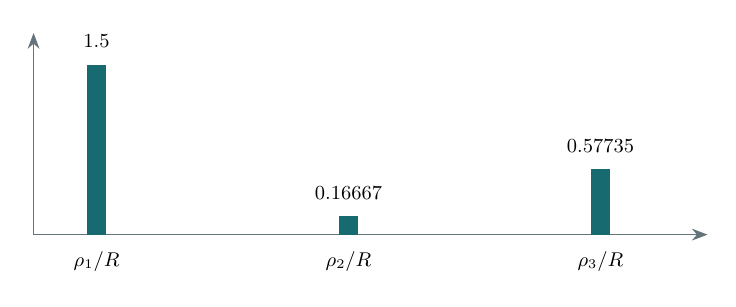
\begin{tikzpicture}[scale=.8,transform shape]
\draw[axis] (0,0)--(10.7,0);
\draw[axis] (0,0)--(0,3.2);
\draw[line width=7pt,color=accent] (1.0,0)--(1.0,2.700000000);
\node[below] at (1.0,-.14) {$\rho_1/R$};
\node[above] at (1.0,2.840000000) {$ 1.5 $};
\draw[line width=7pt,color=accent] (5.0,0)--(5.0,0.300000000);
\node[below] at (5.0,-.14) {$\rho_2/R$};
\node[above] at (5.0,0.440000000) {$ 0.16667 $};
\draw[line width=7pt,color=accent] (9.0,0)--(9.0,1.039230485);
\node[below] at (9.0,-.14) {$\rho_3/R$};
\node[above] at (9.0,1.179230485) {$ 0.57735 $};
\end{tikzpicture}
\figcaption{变图力试2.1V1\quad $M=2m$时三类特殊点的曲率半径}
\end{minipage}\end{center}

\Needspace{20\baselineskip}
\item 取$m=M$，求最低点附近的局部形状，说明曲率公式的极限。
\textbf{解：}变图力试2.1V2中$a=b=R/2$，最低点$\tau=\pi$的速度为零。令$u=\tau-\pi$，有$x-a\pi=a(u-\sin u)=au^3/6+O(u^5)$，$y=a(1-\cos u)=au^2/2+O(u^4)$，形成尖点。邻近光滑支的曲率半径趋零，最低点的零速度使单位切向按两侧分别取极限，轨迹成为带尖点的摆线。
\begin{center}\begin{minipage}{.98\linewidth}\centering
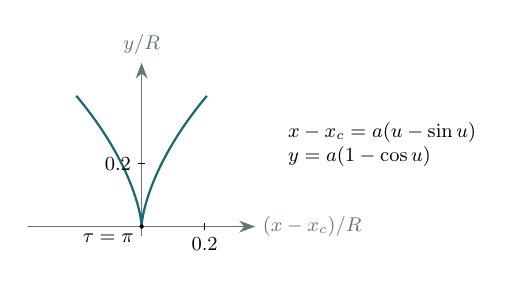
\begin{tikzpicture}[scale=.8,transform shape]
\draw[axis] (-1.8,0)--(1.8,0) node[right] {$(x-x_c)/R$};
\draw[axis] (0,-.15)--(0,2.6) node[above] {$y/R$};
\draw[traj] plot coordinates {(-1.03637568,2.07508214) (-1.00756576,2.04063417) (-0.97923750,2.00627623) (-0.95138958,1.97201506) (-0.92402059,1.93785737) (-0.89712906,1.90380987) (-0.87071337,1.86987921) (-0.84477186,1.83607205) (-0.81930275,1.80239503) (-0.79430416,1.76885473) (-0.76977415,1.73545773) (-0.74571065,1.70221058) (-0.72211152,1.66911979) (-0.69897453,1.63619186) (-0.67629736,1.60343323) (-0.65407758,1.57085032) (-0.63231270,1.53844952) (-0.61100012,1.50623719) (-0.59013715,1.47421962) (-0.56972103,1.44240311) (-0.54974889,1.41079388) (-0.53021780,1.37939814) (-0.51112472,1.34822203) (-0.49246653,1.31727166) (-0.47424003,1.28655310) (-0.45644194,1.25607238) (-0.43906887,1.22583546) (-0.42211738,1.19584828) (-0.40558392,1.16611670) (-0.38946489,1.13664656) (-0.37375657,1.10744363) (-0.35845519,1.07851364) (-0.34355689,1.04986226) (-0.32905772,1.02149510) (-0.31495368,0.99341772) (-0.30124065,0.96563563) (-0.28791448,0.93815426) (-0.27497090,0.91097902) (-0.26240561,0.88411521) (-0.25021420,0.85756812) (-0.23839220,0.83134294) (-0.22693507,0.80544480) (-0.21583820,0.77987880) (-0.20509689,0.75464993) (-0.19470640,0.72976315) (-0.18466190,0.70522333) (-0.17495851,0.68103527) (-0.16559125,0.65720373) (-0.15655512,0.63373337) (-0.14784501,0.61062880) (-0.13945578,0.58789453) (-0.13138221,0.56553503) (-0.12361903,0.54355468) (-0.11616089,0.52195779) (-0.10900240,0.50074859) (-0.10213811,0.47993123) (-0.09556248,0.45950980) (-0.08926996,0.43948830) (-0.08325493,0.41987065) (-0.07751168,0.40066071) (-0.07203451,0.38186222) (-0.06681760,0.36347889) (-0.06185514,0.34551430) (-0.05714123,0.32797199) (-0.05266994,0.31085539) (-0.04843528,0.29416785) (-0.04443122,0.27791265) (-0.04065169,0.26209298) (-0.03709057,0.24671192) (-0.03374170,0.23177250) (-0.03059887,0.21727765) (-0.02765584,0.20323020) (-0.02490632,0.18963292) (-0.02234400,0.17648845) (-0.01996252,0.16379939) (-0.01775548,0.15156822) (-0.01571646,0.13979733) (-0.01383900,0.12848903) (-0.01211660,0.11764554) (-0.01054274,0.10726899) (-0.00911088,0.09736140) (-0.00781443,0.08792473) (-0.00664678,0.07896081) (-0.00560131,0.07047141) (-0.00467136,0.06245819) (-0.00385025,0.05492271) (-0.00313129,0.04786647) (-0.00250775,0.04129083) (-0.00197289,0.03519710) (-0.00151997,0.02958646) (-0.00114221,0.02446001) (-0.00083283,0.01981876) (-0.00058502,0.01566362) (-0.00039198,0.01199540) (-0.00024687,0.00881482) (-0.00014288,0.00612250) (-0.00007316,0.00391898) (-0.00003087,0.00220468) (-0.00000915,0.00097994) (-0.00000114,0.00024500) (0.00000000,0.00000000) (0.00000114,0.00024500) (0.00000915,0.00097994) (0.00003087,0.00220468) (0.00007316,0.00391898) (0.00014288,0.00612250) (0.00024687,0.00881482) (0.00039198,0.01199540) (0.00058502,0.01566362) (0.00083283,0.01981876) (0.00114221,0.02446001) (0.00151997,0.02958646) (0.00197289,0.03519710) (0.00250775,0.04129083) (0.00313129,0.04786647) (0.00385025,0.05492271) (0.00467136,0.06245819) (0.00560131,0.07047141) (0.00664678,0.07896081) (0.00781443,0.08792473) (0.00911088,0.09736140) (0.01054274,0.10726899) (0.01211660,0.11764554) (0.01383900,0.12848903) (0.01571646,0.13979733) (0.01775548,0.15156822) (0.01996252,0.16379939) (0.02234400,0.17648845) (0.02490632,0.18963292) (0.02765584,0.20323020) (0.03059887,0.21727765) (0.03374170,0.23177250) (0.03709057,0.24671192) (0.04065169,0.26209298) (0.04443122,0.27791265) (0.04843528,0.29416785) (0.05266994,0.31085539) (0.05714123,0.32797199) (0.06185514,0.34551430) (0.06681760,0.36347889) (0.07203451,0.38186222) (0.07751168,0.40066071) (0.08325493,0.41987065) (0.08926996,0.43948830) (0.09556248,0.45950980) (0.10213811,0.47993123) (0.10900240,0.50074859) (0.11616089,0.52195779) (0.12361903,0.54355468) (0.13138221,0.56553503) (0.13945578,0.58789453) (0.14784501,0.61062880) (0.15655512,0.63373337) (0.16559125,0.65720373) (0.17495851,0.68103527) (0.18466190,0.70522333) (0.19470640,0.72976315) (0.20509689,0.75464993) (0.21583820,0.77987880) (0.22693507,0.80544480) (0.23839220,0.83134294) (0.25021420,0.85756812) (0.26240561,0.88411521) (0.27497090,0.91097902) (0.28791448,0.93815426) (0.30124065,0.96563563) (0.31495368,0.99341772) (0.32905772,1.02149510) (0.34355689,1.04986226) (0.35845519,1.07851364) (0.37375657,1.10744363) (0.38946489,1.13664656) (0.40558392,1.16611670) (0.42211738,1.19584828) (0.43906887,1.22583546) (0.45644194,1.25607238) (0.47424003,1.28655310) (0.49246653,1.31727166) (0.51112472,1.34822203) (0.53021780,1.37939814) (0.54974889,1.41079388) (0.56972103,1.44240311) (0.59013715,1.47421962) (0.61100012,1.50623719) (0.63231270,1.53844952) (0.65407758,1.57085032) (0.67629736,1.60343323) (0.69897453,1.63619186) (0.72211152,1.66911979) (0.74571065,1.70221058) (0.76977415,1.73545773) (0.79430416,1.76885473) (0.81930275,1.80239503) (0.84477186,1.83607205) (0.87071337,1.86987921) (0.89712906,1.90380987) (0.92402059,1.93785737) (0.95138958,1.97201506) (0.97923750,2.00627623) (1.00756576,2.04063417) (1.03637568,2.07508214)};
\fill (0,0) circle(.035);
\node[below left] at (0,0) {$\tau=\pi$};
\draw[thin] (-.06,1)--(.06,1) node[left,xshift=-3pt] {$0.2$};
\draw[thin] (1,-.06)--(1,.06) node[below,yshift=-3pt] {$0.2$};
\node[right,align=left] at (2.2,1.3) {$x-x_c=a(u-\sin u)$\\$y=a(1-\cos u)$};
\end{tikzpicture}
\figcaption{变图力试2.1V2\quad 两侧光滑支在最低点形成零速度尖点}
\end{minipage}\end{center}

\Needspace{20\baselineskip}
\item 改取$m>M$，判断环套、竖直切线和拐点，写一般曲率半径。
\textbf{解：}变图力试2.1V3有$a<b$，$v_x=\omega(b+a\cos\tau)>0$，轨迹向右单调展开，环套与竖直切线消失。参数曲率半径为$(a^2+b^2+2ab\cos\tau)^{3/2}/[a|a+b\cos\tau|]$。当$\cos\tau=-a/b=-M/m$时分母为零、速度仍非零，出现拐点，曲率为零、曲率半径趋无穷。绝对值保留曲率半径的非负大小。
\begin{center}\begin{minipage}{.98\linewidth}\centering
\begin{tikzpicture}[scale=.8,transform shape]
\draw[axis] (0,0)--(7.5,0) node[right] {$x$};
\draw[axis] (0,0)--(0,2.1) node[above] {$y$};
\draw[traj] plot coordinates {(0.00000000,1.65000000) (0.04319525,1.64981153) (0.08638064,1.64924624) (0.12954630,1.64830453) (0.17268239,1.64698704) (0.21577907,1.64529467) (0.25882655,1.64322859) (0.30181507,1.64079020) (0.34473489,1.63798118) (0.38757634,1.63480346) (0.43032980,1.63125920) (0.47298570,1.62735085) (0.51553454,1.62308108) (0.55796690,1.61845282) (0.60027343,1.61346923) (0.64244488,1.60813374) (0.68447208,1.60245000) (0.72634596,1.59642191) (0.76805756,1.59005359) (0.80959804,1.58334941) (0.85095865,1.57631397) (0.89213080,1.56895209) (0.93310599,1.56126881) (0.97387588,1.55326940) (1.01443227,1.54495935) (1.05476710,1.53634434) (1.09487246,1.52743028) (1.13474061,1.51822328) (1.17436395,1.50872965) (1.21373506,1.49895590) (1.25284671,1.48890873) (1.29169182,1.47859502) (1.33026350,1.46802183) (1.36855506,1.45719643) (1.40655999,1.44612622) (1.44427198,1.43481879) (1.48168492,1.42328189) (1.51879291,1.41152343) (1.55559025,1.39955147) (1.59207146,1.38737421) (1.62823128,1.37500000) (1.66406465,1.36243732) (1.69956676,1.34969477) (1.73473301,1.33678110) (1.76955904,1.32370515) (1.80404071,1.31047589) (1.83817414,1.29710237) (1.87195566,1.28359377) (1.90538185,1.26995935) (1.93844955,1.25620844) (1.97115584,1.24235047) (2.00349802,1.22839495) (2.03547368,1.21435143) (2.06708063,1.20022954) (2.09831695,1.18603896) (2.12918097,1.17178941) (2.15967127,1.15749065) (2.18978670,1.14315250) (2.21952634,1.12878478) (2.24888956,1.11439732) (2.27787596,1.10000000) (2.30648542,1.08560268) (2.33471807,1.07121522) (2.36257429,1.05684750) (2.39005473,1.04250935) (2.41716030,1.02821059) (2.44389214,1.01396104) (2.47025169,0.99977046) (2.49624060,0.98564857) (2.52186081,0.97160505) (2.54711449,0.95764953) (2.57200407,0.94379156) (2.59653224,0.93004065) (2.62070190,0.91640623) (2.64451625,0.90289763) (2.66797869,0.88952411) (2.69109288,0.87629485) (2.71386272,0.86321890) (2.73629234,0.85030523) (2.75838609,0.83756268) (2.78014858,0.82500000) (2.80158464,0.81262579) (2.82269929,0.80044853) (2.84349781,0.78847657) (2.86398569,0.77671811) (2.88416861,0.76518121) (2.90405249,0.75387378) (2.92364342,0.74280357) (2.94294773,0.73197817) (2.96197191,0.72140498) (2.98072267,0.71109127) (2.99920689,0.70104410) (3.01743164,0.69127035) (3.03540416,0.68177672) (3.05313188,0.67256972) (3.07062239,0.66365566) (3.08788342,0.65504065) (3.10492290,0.64673060) (3.12174887,0.63873119) (3.13836954,0.63104791) (3.15479327,0.62368603) (3.17102852,0.61665059) (3.18708391,0.60994641) (3.20296817,0.60357809) (3.21869015,0.59755000) (3.23425882,0.59186626) (3.24968323,0.58653077) (3.26497257,0.58154718) (3.28013607,0.57691892) (3.29518310,0.57264915) (3.31012307,0.56874080) (3.32496548,0.56519654) (3.33971989,0.56201882) (3.35439593,0.55920980) (3.36900328,0.55677141) (3.38355166,0.55470533) (3.39805084,0.55301296) (3.41251062,0.55169547) (3.42694083,0.55075376) (3.44135131,0.55018847) (3.45575192,0.55000000) (3.47015253,0.55018847) (3.48456301,0.55075376) (3.49899321,0.55169547) (3.51345299,0.55301296) (3.52795218,0.55470533) (3.54250056,0.55677141) (3.55710791,0.55920980) (3.57178395,0.56201882) (3.58653836,0.56519654) (3.60138077,0.56874080) (3.61632074,0.57264915) (3.63136776,0.57691892) (3.64653127,0.58154718) (3.66182060,0.58653077) (3.67724502,0.59186626) (3.69281369,0.59755000) (3.70853567,0.60357809) (3.72441993,0.60994641) (3.74047532,0.61665059) (3.75671057,0.62368603) (3.77313429,0.63104791) (3.78975497,0.63873119) (3.80658094,0.64673060) (3.82362041,0.65504065) (3.84088145,0.66365566) (3.85837195,0.67256972) (3.87609967,0.68177672) (3.89407220,0.69127035) (3.91229695,0.70104410) (3.93078117,0.71109127) (3.94953193,0.72140498) (3.96855611,0.73197817) (3.98786042,0.74280357) (4.00745135,0.75387378) (4.02733522,0.76518121) (4.04751815,0.77671811) (4.06800602,0.78847657) (4.08880455,0.80044853) (4.10991920,0.81262579) (4.13135525,0.82500000) (4.15311775,0.83756268) (4.17521150,0.85030523) (4.19764112,0.86321890) (4.22041095,0.87629485) (4.24352515,0.88952411) (4.26698759,0.90289763) (4.29080193,0.91640623) (4.31497160,0.93004065) (4.33949977,0.94379156) (4.36438935,0.95764953) (4.38964303,0.97160505) (4.41526324,0.98564857) (4.44125215,0.99977046) (4.46761170,1.01396104) (4.49434354,1.02821059) (4.52144911,1.04250935) (4.54892955,1.05684750) (4.57678577,1.07121522) (4.60501842,1.08560268) (4.63362788,1.10000000) (4.66261428,1.11439732) (4.69197750,1.12878478) (4.72171714,1.14315250) (4.75183257,1.15749065) (4.78232287,1.17178941) (4.81318689,1.18603896) (4.84442321,1.20022954) (4.87603016,1.21435143) (4.90800582,1.22839495) (4.94034800,1.24235047) (4.97305428,1.25620844) (5.00612199,1.26995935) (5.03954818,1.28359377) (5.07332970,1.29710237) (5.10746313,1.31047589) (5.14194480,1.32370515) (5.17677083,1.33678110) (5.21193708,1.34969477) (5.24743919,1.36243732) (5.28327256,1.37500000) (5.31943237,1.38737421) (5.35591358,1.39955147) (5.39271093,1.41152343) (5.42981892,1.42328189) (5.46723186,1.43481879) (5.50494385,1.44612622) (5.54294878,1.45719643) (5.58124034,1.46802183) (5.61981202,1.47859502) (5.65865713,1.48890873) (5.69776877,1.49895590) (5.73713989,1.50872965) (5.77676323,1.51822328) (5.81663137,1.52743028) (5.85673674,1.53634434) (5.89707157,1.54495935) (5.93762796,1.55326940) (5.97839785,1.56126881) (6.01937304,1.56895209) (6.06054518,1.57631397) (6.10190580,1.58334941) (6.14344628,1.59005359) (6.18515788,1.59642191) (6.22703176,1.60245000) (6.26905896,1.60813374) (6.31123041,1.61346923) (6.35353694,1.61845282) (6.39596930,1.62308108) (6.43851814,1.62735085) (6.48117404,1.63125920) (6.52392749,1.63480346) (6.56676895,1.63798118) (6.60968877,1.64079020) (6.65267729,1.64322859) (6.69572477,1.64529467) (6.73882145,1.64698704) (6.78195754,1.64830453) (6.82512320,1.64924624) (6.86830858,1.64981153) (6.91150384,1.65000000)};
\node[above] at (3.5,2.1) {$m=2M,\quad a=R/3,\ b=2R/3$};
\fill[color=warm] (2.78014858,0.82500000) circle(.04);
\fill[color=warm] (4.13135525,0.82500000) circle(.04);
\node[below,align=center] at (3.45,.35) {两点均满足$\cos\tau=-1/2$\\法向加速度为零，弯曲方向改变};
\end{tikzpicture}
\figcaption{变图力试2.1V3\quad 质点更重时轨迹无环套，并在局部弯曲方向改变处出现拐点}
\end{minipage}\end{center}

\Needspace{20\baselineskip}
\item 给整个系统初始运动叠加匀速$U\hat x$，求接触和环套条件的变化。
\textbf{解：}变图力试2.1V4中相对速度和$\omega$保持，所需支持力也保持。地面方程改为$x=(V_C+U)t+a\sin\omega t$，$y=b+a\cos\omega t$。令$W=V_C+U$，$v_x=W+a\omega\cos\tau$，当$0<|W|<a\omega$时出现带匀速推进的环套；$W=0$时质心在该系静止，轨迹为半径$a$的圆。$|W|=a\omega$时出现零速度尖点，$|W|>a\omega$时水平速度保持同号。环套形态与曲率由所选观察惯性系决定。
\begin{center}\begin{minipage}{.98\linewidth}\centering
\begin{tikzpicture}[scale=.72,transform shape]
\draw[thin,color=muted] (-.7,-0.0000)--(5.6,-0.0000);
\draw[traj] plot coordinates {(0.00000000,0.55000000) (0.01439732,0.54981153) (0.02878478,0.54924624) (0.04315250,0.54830453) (0.05749065,0.54698704) (0.07178941,0.54529467) (0.08603896,0.54322859) (0.10022954,0.54079020) (0.11435143,0.53798118) (0.12839495,0.53480346) (0.14235047,0.53125920) (0.15620844,0.52735085) (0.16995935,0.52308108) (0.18359377,0.51845282) (0.19710237,0.51346923) (0.21047589,0.50813374) (0.22370515,0.50245000) (0.23678110,0.49642191) (0.24969477,0.49005359) (0.26243732,0.48334941) (0.27500000,0.47631397) (0.28737421,0.46895209) (0.29955147,0.46126881) (0.31152343,0.45326940) (0.32328189,0.44495935) (0.33481879,0.43634434) (0.34612622,0.42743028) (0.35719643,0.41822328) (0.36802183,0.40872965) (0.37859502,0.39895590) (0.38890873,0.38890873) (0.39895590,0.37859502) (0.40872965,0.36802183) (0.41822328,0.35719643) (0.42743028,0.34612622) (0.43634434,0.33481879) (0.44495935,0.32328189) (0.45326940,0.31152343) (0.46126881,0.29955147) (0.46895209,0.28737421) (0.47631397,0.27500000) (0.48334941,0.26243732) (0.49005359,0.24969477) (0.49642191,0.23678110) (0.50245000,0.22370515) (0.50813374,0.21047589) (0.51346923,0.19710237) (0.51845282,0.18359377) (0.52308108,0.16995935) (0.52735085,0.15620844) (0.53125920,0.14235047) (0.53480346,0.12839495) (0.53798118,0.11435143) (0.54079020,0.10022954) (0.54322859,0.08603896) (0.54529467,0.07178941) (0.54698704,0.05749065) (0.54830453,0.04315250) (0.54924624,0.02878478) (0.54981153,0.01439732) (0.55000000,0.00000000) (0.54981153,-0.01439732) (0.54924624,-0.02878478) (0.54830453,-0.04315250) (0.54698704,-0.05749065) (0.54529467,-0.07178941) (0.54322859,-0.08603896) (0.54079020,-0.10022954) (0.53798118,-0.11435143) (0.53480346,-0.12839495) (0.53125920,-0.14235047) (0.52735085,-0.15620844) (0.52308108,-0.16995935) (0.51845282,-0.18359377) (0.51346923,-0.19710237) (0.50813374,-0.21047589) (0.50245000,-0.22370515) (0.49642191,-0.23678110) (0.49005359,-0.24969477) (0.48334941,-0.26243732) (0.47631397,-0.27500000) (0.46895209,-0.28737421) (0.46126881,-0.29955147) (0.45326940,-0.31152343) (0.44495935,-0.32328189) (0.43634434,-0.33481879) (0.42743028,-0.34612622) (0.41822328,-0.35719643) (0.40872965,-0.36802183) (0.39895590,-0.37859502) (0.38890873,-0.38890873) (0.37859502,-0.39895590) (0.36802183,-0.40872965) (0.35719643,-0.41822328) (0.34612622,-0.42743028) (0.33481879,-0.43634434) (0.32328189,-0.44495935) (0.31152343,-0.45326940) (0.29955147,-0.46126881) (0.28737421,-0.46895209) (0.27500000,-0.47631397) (0.26243732,-0.48334941) (0.24969477,-0.49005359) (0.23678110,-0.49642191) (0.22370515,-0.50245000) (0.21047589,-0.50813374) (0.19710237,-0.51346923) (0.18359377,-0.51845282) (0.16995935,-0.52308108) (0.15620844,-0.52735085) (0.14235047,-0.53125920) (0.12839495,-0.53480346) (0.11435143,-0.53798118) (0.10022954,-0.54079020) (0.08603896,-0.54322859) (0.07178941,-0.54529467) (0.05749065,-0.54698704) (0.04315250,-0.54830453) (0.02878478,-0.54924624) (0.01439732,-0.54981153) (0.00000000,-0.55000000) (-0.01439732,-0.54981153) (-0.02878478,-0.54924624) (-0.04315250,-0.54830453) (-0.05749065,-0.54698704) (-0.07178941,-0.54529467) (-0.08603896,-0.54322859) (-0.10022954,-0.54079020) (-0.11435143,-0.53798118) (-0.12839495,-0.53480346) (-0.14235047,-0.53125920) (-0.15620844,-0.52735085) (-0.16995935,-0.52308108) (-0.18359377,-0.51845282) (-0.19710237,-0.51346923) (-0.21047589,-0.50813374) (-0.22370515,-0.50245000) (-0.23678110,-0.49642191) (-0.24969477,-0.49005359) (-0.26243732,-0.48334941) (-0.27500000,-0.47631397) (-0.28737421,-0.46895209) (-0.29955147,-0.46126881) (-0.31152343,-0.45326940) (-0.32328189,-0.44495935) (-0.33481879,-0.43634434) (-0.34612622,-0.42743028) (-0.35719643,-0.41822328) (-0.36802183,-0.40872965) (-0.37859502,-0.39895590) (-0.38890873,-0.38890873) (-0.39895590,-0.37859502) (-0.40872965,-0.36802183) (-0.41822328,-0.35719643) (-0.42743028,-0.34612622) (-0.43634434,-0.33481879) (-0.44495935,-0.32328189) (-0.45326940,-0.31152343) (-0.46126881,-0.29955147) (-0.46895209,-0.28737421) (-0.47631397,-0.27500000) (-0.48334941,-0.26243732) (-0.49005359,-0.24969477) (-0.49642191,-0.23678110) (-0.50245000,-0.22370515) (-0.50813374,-0.21047589) (-0.51346923,-0.19710237) (-0.51845282,-0.18359377) (-0.52308108,-0.16995935) (-0.52735085,-0.15620844) (-0.53125920,-0.14235047) (-0.53480346,-0.12839495) (-0.53798118,-0.11435143) (-0.54079020,-0.10022954) (-0.54322859,-0.08603896) (-0.54529467,-0.07178941) (-0.54698704,-0.05749065) (-0.54830453,-0.04315250) (-0.54924624,-0.02878478) (-0.54981153,-0.01439732) (-0.55000000,-0.00000000) (-0.54981153,0.01439732) (-0.54924624,0.02878478) (-0.54830453,0.04315250) (-0.54698704,0.05749065) (-0.54529467,0.07178941) (-0.54322859,0.08603896) (-0.54079020,0.10022954) (-0.53798118,0.11435143) (-0.53480346,0.12839495) (-0.53125920,0.14235047) (-0.52735085,0.15620844) (-0.52308108,0.16995935) (-0.51845282,0.18359377) (-0.51346923,0.19710237) (-0.50813374,0.21047589) (-0.50245000,0.22370515) (-0.49642191,0.23678110) (-0.49005359,0.24969477) (-0.48334941,0.26243732) (-0.47631397,0.27500000) (-0.46895209,0.28737421) (-0.46126881,0.29955147) (-0.45326940,0.31152343) (-0.44495935,0.32328189) (-0.43634434,0.33481879) (-0.42743028,0.34612622) (-0.41822328,0.35719643) (-0.40872965,0.36802183) (-0.39895590,0.37859502) (-0.38890873,0.38890873) (-0.37859502,0.39895590) (-0.36802183,0.40872965) (-0.35719643,0.41822328) (-0.34612622,0.42743028) (-0.33481879,0.43634434) (-0.32328189,0.44495935) (-0.31152343,0.45326940) (-0.29955147,0.46126881) (-0.28737421,0.46895209) (-0.27500000,0.47631397) (-0.26243732,0.48334941) (-0.24969477,0.49005359) (-0.23678110,0.49642191) (-0.22370515,0.50245000) (-0.21047589,0.50813374) (-0.19710237,0.51346923) (-0.18359377,0.51845282) (-0.16995935,0.52308108) (-0.15620844,0.52735085) (-0.14235047,0.53125920) (-0.12839495,0.53480346) (-0.11435143,0.53798118) (-0.10022954,0.54079020) (-0.08603896,0.54322859) (-0.07178941,0.54529467) (-0.05749065,0.54698704) (-0.04315250,0.54830453) (-0.02878478,0.54924624) (-0.01439732,0.54981153) (-0.00000000,0.55000000)};
\node[right,align=left] at (6,-0.0000) {$W/(a\omega)=0$\\圆};
\draw[thin,color=muted] (-.7,-2.4000)--(5.6,-2.4000);
\draw[traj] plot coordinates {(0.00000000,-1.85000000) (0.02159680,-1.85018847) (0.04318374,-1.85075376) (0.06475095,-1.85169547) (0.08628859,-1.85301296) (0.10778682,-1.85470533) (0.12923585,-1.85677141) (0.15062592,-1.85920980) (0.17194730,-1.86201882) (0.19319030,-1.86519654) (0.21434531,-1.86874080) (0.23540275,-1.87264915) (0.25635314,-1.87691892) (0.27718705,-1.88154718) (0.29789514,-1.88653077) (0.31846814,-1.89186626) (0.33889688,-1.89755000) (0.35917232,-1.90357809) (0.37928547,-1.90994641) (0.39922750,-1.91665059) (0.41898966,-1.92368603) (0.43856336,-1.93104791) (0.45794010,-1.93873119) (0.47711154,-1.94673060) (0.49606948,-1.95504065) (0.51480587,-1.96365566) (0.53331278,-1.97256972) (0.55158247,-1.98177672) (0.56960736,-1.99127035) (0.58738003,-2.00104410) (0.60489322,-2.01109127) (0.62213988,-2.02140498) (0.63911312,-2.03197817) (0.65580623,-2.04280357) (0.67221271,-2.05387378) (0.68832625,-2.06518121) (0.70414074,-2.07671811) (0.71965028,-2.08847657) (0.73484917,-2.10044853) (0.74973193,-2.11262579) (0.76429330,-2.12500000) (0.77852822,-2.13756268) (0.79243188,-2.15030523) (0.80599968,-2.16321890) (0.81922726,-2.17629485) (0.83211049,-2.18952411) (0.84464546,-2.20289763) (0.85682853,-2.21640623) (0.86865628,-2.23004065) (0.88012553,-2.24379156) (0.89123336,-2.25764953) (0.90197710,-2.27160505) (0.91235430,-2.28564857) (0.92236281,-2.29977046) (0.93200068,-2.31396104) (0.94126625,-2.32821059) (0.95015810,-2.34250935) (0.95867507,-2.35684750) (0.96681627,-2.37121522) (0.97458104,-2.38560268) (0.98196899,-2.40000000) (0.98898000,-2.41439732) (0.99561420,-2.42878478) (1.00187197,-2.44315250) (1.00775396,-2.45749065) (1.01326108,-2.47178941) (1.01839448,-2.48603896) (1.02315557,-2.50022954) (1.02754604,-2.51435143) (1.03156779,-2.52839495) (1.03522303,-2.54235047) (1.03851416,-2.55620844) (1.04144387,-2.56995935) (1.04401509,-2.58359377) (1.04623099,-2.59710237) (1.04809498,-2.61047589) (1.04961072,-2.62370515) (1.05078211,-2.63678110) (1.05161328,-2.64969477) (1.05210858,-2.66243732) (1.05227263,-2.67500000) (1.05211023,-2.68737421) (1.05162643,-2.69955147) (1.05082651,-2.71152343) (1.04971593,-2.72328189) (1.04830041,-2.73481879) (1.04658583,-2.74612622) (1.04457832,-2.75719643) (1.04228417,-2.76802183) (1.03970991,-2.77859502) (1.03686221,-2.78890873) (1.03374798,-2.79895590) (1.03037428,-2.80872965) (1.02674836,-2.81822328) (1.02287763,-2.82743028) (1.01876969,-2.83634434) (1.01443227,-2.84495935) (1.00987330,-2.85326940) (1.00510082,-2.86126881) (1.00012304,-2.86895209) (0.99494832,-2.87631397) (0.98958512,-2.88334941) (0.98404206,-2.89005359) (0.97832787,-2.89642191) (0.97245140,-2.90245000) (0.96642162,-2.90813374) (0.96024759,-2.91346923) (0.95393847,-2.91845282) (0.94750353,-2.92308108) (0.94095210,-2.92735085) (0.93429362,-2.93125920) (0.92753758,-2.93480346) (0.92069354,-2.93798118) (0.91377114,-2.94079020) (0.90678004,-2.94322859) (0.89972997,-2.94529467) (0.89263070,-2.94698704) (0.88549203,-2.94830453) (0.87832379,-2.94924624) (0.87113582,-2.94981153) (0.86393798,-2.95000000) (0.85674014,-2.94981153) (0.84955217,-2.94924624) (0.84238393,-2.94830453) (0.83524526,-2.94698704) (0.82814599,-2.94529467) (0.82109592,-2.94322859) (0.81410482,-2.94079020) (0.80718242,-2.93798118) (0.80033838,-2.93480346) (0.79358234,-2.93125920) (0.78692385,-2.92735085) (0.78037243,-2.92308108) (0.77393749,-2.91845282) (0.76762837,-2.91346923) (0.76145434,-2.90813374) (0.75542456,-2.90245000) (0.74954809,-2.89642191) (0.74383390,-2.89005359) (0.73829084,-2.88334941) (0.73292764,-2.87631397) (0.72775292,-2.86895209) (0.72277514,-2.86126881) (0.71800266,-2.85326940) (0.71344369,-2.84495935) (0.70910627,-2.83634434) (0.70499833,-2.82743028) (0.70112760,-2.81822328) (0.69750167,-2.80872965) (0.69412797,-2.79895590) (0.69101375,-2.78890873) (0.68816605,-2.77859502) (0.68559179,-2.76802183) (0.68329764,-2.75719643) (0.68129013,-2.74612622) (0.67957555,-2.73481879) (0.67816003,-2.72328189) (0.67704945,-2.71152343) (0.67624953,-2.69955147) (0.67576573,-2.68737421) (0.67560333,-2.67500000) (0.67576738,-2.66243732) (0.67626268,-2.64969477) (0.67709385,-2.63678110) (0.67826524,-2.62370515) (0.67978098,-2.61047589) (0.68164497,-2.59710237) (0.68386087,-2.58359377) (0.68643209,-2.56995935) (0.68936180,-2.55620844) (0.69265293,-2.54235047) (0.69630816,-2.52839495) (0.70032992,-2.51435143) (0.70472039,-2.50022954) (0.70948148,-2.48603896) (0.71461488,-2.47178941) (0.72012199,-2.45749065) (0.72600399,-2.44315250) (0.73226176,-2.42878478) (0.73889596,-2.41439732) (0.74590697,-2.40000000) (0.75329492,-2.38560268) (0.76105969,-2.37121522) (0.76920089,-2.35684750) (0.77771786,-2.34250935) (0.78660971,-2.32821059) (0.79587528,-2.31396104) (0.80551315,-2.29977046) (0.81552165,-2.28564857) (0.82589886,-2.27160505) (0.83664260,-2.25764953) (0.84775043,-2.24379156) (0.85921968,-2.23004065) (0.87104743,-2.21640623) (0.88323050,-2.20289763) (0.89576547,-2.18952411) (0.90864870,-2.17629485) (0.92187628,-2.16321890) (0.93544408,-2.15030523) (0.94934774,-2.13756268) (0.96358266,-2.12500000) (0.97814403,-2.11262579) (0.99302679,-2.10044853) (1.00822568,-2.08847657) (1.02373522,-2.07671811) (1.03954971,-2.06518121) (1.05566325,-2.05387378) (1.07206973,-2.04280357) (1.08876284,-2.03197817) (1.10573608,-2.02140498) (1.12298273,-2.01109127) (1.14049593,-2.00104410) (1.15826860,-1.99127035) (1.17629349,-1.98177672) (1.19456318,-1.97256972) (1.21307009,-1.96365566) (1.23180647,-1.95504065) (1.25076442,-1.94673060) (1.26993586,-1.93873119) (1.28931260,-1.93104791) (1.30888630,-1.92368603) (1.32864846,-1.91665059) (1.34859049,-1.90994641) (1.36870364,-1.90357809) (1.38897908,-1.89755000) (1.40940782,-1.89186626) (1.42998082,-1.88653077) (1.45068891,-1.88154718) (1.47152281,-1.87691892) (1.49247321,-1.87264915) (1.51353065,-1.86874080) (1.53468566,-1.86519654) (1.55592866,-1.86201882) (1.57725004,-1.85920980) (1.59864010,-1.85677141) (1.62008914,-1.85470533) (1.64158737,-1.85301296) (1.66312501,-1.85169547) (1.68469222,-1.85075376) (1.70627915,-1.85018847) (1.72787596,-1.85000000)};
\node[right,align=left] at (6,-2.4000) {$W/(a\omega)=0.5$\\环套};
\draw[thin,color=muted] (-.7,-4.8000)--(5.6,-4.8000);
\draw[traj] plot coordinates {(0.00000000,-4.25000000) (0.02879629,-4.25018847) (0.05758271,-4.25075376) (0.08634940,-4.25169547) (0.11508652,-4.25301296) (0.14378424,-4.25470533) (0.17243275,-4.25677141) (0.20102230,-4.25920980) (0.22954316,-4.26201882) (0.25798565,-4.26519654) (0.28634014,-4.26874080) (0.31459707,-4.27264915) (0.34274694,-4.27691892) (0.37078033,-4.28154718) (0.39868790,-4.28653077) (0.42646038,-4.29186626) (0.45408861,-4.29755000) (0.48156353,-4.30357809) (0.50887617,-4.30994641) (0.53601768,-4.31665059) (0.56297933,-4.32368603) (0.58975250,-4.33104791) (0.61632873,-4.33873119) (0.64269966,-4.34673060) (0.66885708,-4.35504065) (0.69479294,-4.36365566) (0.72049934,-4.37256972) (0.74596852,-4.38177672) (0.77119289,-4.39127035) (0.79616504,-4.40104410) (0.82087772,-4.41109127) (0.84532386,-4.42140498) (0.86949658,-4.43197817) (0.89338917,-4.44280357) (0.91699513,-4.45387378) (0.94030816,-4.46518121) (0.96332213,-4.47671811) (0.98603116,-4.48847657) (1.00842953,-4.50044853) (1.03051178,-4.51262579) (1.05227263,-4.52500000) (1.07370703,-4.53756268) (1.09481017,-4.55030523) (1.11557746,-4.56321890) (1.13600452,-4.57629485) (1.15608723,-4.58952411) (1.17582169,-4.60289763) (1.19520424,-4.61640623) (1.21423147,-4.63004065) (1.23290020,-4.64379156) (1.25120752,-4.65764953) (1.26915074,-4.67160505) (1.28672743,-4.68564857) (1.30393541,-4.69977046) (1.32077277,-4.71396104) (1.33723782,-4.72821059) (1.35332916,-4.74250935) (1.36904561,-4.75684750) (1.38438629,-4.77121522) (1.39935054,-4.78560268) (1.41393798,-4.80000000) (1.42814847,-4.81439732) (1.44198216,-4.82878478) (1.45543941,-4.84315250) (1.46852089,-4.85749065) (1.48122749,-4.87178941) (1.49356037,-4.88603896) (1.50552094,-4.90022954) (1.51711089,-4.91435143) (1.52833213,-4.92839495) (1.53918685,-4.94235047) (1.54967746,-4.95620844) (1.55980666,-4.96995935) (1.56957736,-4.98359377) (1.57899274,-4.99710237) (1.58805622,-5.01047589) (1.59677144,-5.02370515) (1.60514231,-5.03678110) (1.61317296,-5.04969477) (1.62086775,-5.06243732) (1.62823128,-5.07500000) (1.63526836,-5.08737421) (1.64198405,-5.09955147) (1.64838361,-5.11152343) (1.65447252,-5.12328189) (1.66025648,-5.13481879) (1.66574138,-5.14612622) (1.67093335,-5.15719643) (1.67583869,-5.16802183) (1.68046391,-5.17859502) (1.68481570,-5.18890873) (1.68890095,-5.19895590) (1.69272674,-5.20872965) (1.69630030,-5.21822328) (1.69962905,-5.22743028) (1.70272059,-5.23634434) (1.70558266,-5.24495935) (1.70822316,-5.25326940) (1.71065017,-5.26126881) (1.71287188,-5.26895209) (1.71489663,-5.27631397) (1.71673292,-5.28334941) (1.71838934,-5.29005359) (1.71987464,-5.29642191) (1.72119765,-5.30245000) (1.72236735,-5.30813374) (1.72339280,-5.31346923) (1.72428317,-5.31845282) (1.72504771,-5.32308108) (1.72569577,-5.32735085) (1.72623677,-5.33125920) (1.72668021,-5.33480346) (1.72703566,-5.33798118) (1.72731273,-5.34079020) (1.72752112,-5.34322859) (1.72767053,-5.34529467) (1.72777075,-5.34698704) (1.72783156,-5.34830453) (1.72786280,-5.34924624) (1.72787431,-5.34981153) (1.72787596,-5.35000000) (1.72787760,-5.34981153) (1.72788912,-5.34924624) (1.72792036,-5.34830453) (1.72798117,-5.34698704) (1.72808139,-5.34529467) (1.72823080,-5.34322859) (1.72843918,-5.34079020) (1.72871626,-5.33798118) (1.72907171,-5.33480346) (1.72951515,-5.33125920) (1.73005615,-5.32735085) (1.73070421,-5.32308108) (1.73146875,-5.31845282) (1.73235912,-5.31346923) (1.73338457,-5.30813374) (1.73455427,-5.30245000) (1.73587728,-5.29642191) (1.73736258,-5.29005359) (1.73901900,-5.28334941) (1.74085529,-5.27631397) (1.74288004,-5.26895209) (1.74510175,-5.26126881) (1.74752875,-5.25326940) (1.75016926,-5.24495935) (1.75303133,-5.23634434) (1.75612287,-5.22743028) (1.75945162,-5.21822328) (1.76302518,-5.20872965) (1.76685097,-5.19895590) (1.77093622,-5.18890873) (1.77528801,-5.17859502) (1.77991323,-5.16802183) (1.78481857,-5.15719643) (1.79001054,-5.14612622) (1.79549544,-5.13481879) (1.80127940,-5.12328189) (1.80736831,-5.11152343) (1.81376787,-5.09955147) (1.82048356,-5.08737421) (1.82752064,-5.07500000) (1.83488417,-5.06243732) (1.84257896,-5.04969477) (1.85060961,-5.03678110) (1.85898048,-5.02370515) (1.86769570,-5.01047589) (1.87675918,-4.99710237) (1.88617456,-4.98359377) (1.89594526,-4.96995935) (1.90607446,-4.95620844) (1.91656507,-4.94235047) (1.92741979,-4.92839495) (1.93864103,-4.91435143) (1.95023098,-4.90022954) (1.96219155,-4.88603896) (1.97452443,-4.87178941) (1.98723103,-4.85749065) (2.00031251,-4.84315250) (2.01376976,-4.82878478) (2.02760344,-4.81439732) (2.04181394,-4.80000000) (2.05640138,-4.78560268) (2.07136563,-4.77121522) (2.08670630,-4.75684750) (2.10242276,-4.74250935) (2.11851410,-4.72821059) (2.13497915,-4.71396104) (2.15181650,-4.69977046) (2.16902449,-4.68564857) (2.18660118,-4.67160505) (2.20454440,-4.65764953) (2.22285171,-4.64379156) (2.24152045,-4.63004065) (2.26054768,-4.61640623) (2.27993023,-4.60289763) (2.29966469,-4.58952411) (2.31974740,-4.57629485) (2.34017446,-4.56321890) (2.36094174,-4.55030523) (2.38204489,-4.53756268) (2.40347929,-4.52500000) (2.42524014,-4.51262579) (2.44732239,-4.50044853) (2.46972076,-4.48847657) (2.49242978,-4.47671811) (2.51544376,-4.46518121) (2.53875678,-4.45387378) (2.56236275,-4.44280357) (2.58625534,-4.43197817) (2.61042806,-4.42140498) (2.63487420,-4.41109127) (2.65958688,-4.40104410) (2.68455903,-4.39127035) (2.70978340,-4.38177672) (2.73525258,-4.37256972) (2.76095897,-4.36365566) (2.78689484,-4.35504065) (2.81305226,-4.34673060) (2.83942319,-4.33873119) (2.86599942,-4.33104791) (2.89277259,-4.32368603) (2.91973424,-4.31665059) (2.94687575,-4.30994641) (2.97418839,-4.30357809) (3.00166330,-4.29755000) (3.02929154,-4.29186626) (3.05706402,-4.28653077) (3.08497158,-4.28154718) (3.11300498,-4.27691892) (3.14115485,-4.27264915) (3.16941178,-4.26874080) (3.19776627,-4.26519654) (3.22620876,-4.26201882) (3.25472962,-4.25920980) (3.28331917,-4.25677141) (3.31196768,-4.25470533) (3.34066540,-4.25301296) (3.36940252,-4.25169547) (3.39816921,-4.25075376) (3.42695563,-4.25018847) (3.45575192,-4.25000000)};
\node[right,align=left] at (6,-4.8000) {$W/(a\omega)=1$\\尖点};
\draw[thin,color=muted] (-.7,-7.2000)--(5.6,-7.2000);
\draw[traj] plot coordinates {(0.00000000,-6.65000000) (0.03599577,-6.65018847) (0.07198167,-6.65075376) (0.10794785,-6.65169547) (0.14388445,-6.65301296) (0.17978165,-6.65470533) (0.21562965,-6.65677141) (0.25141869,-6.65920980) (0.28713903,-6.66201882) (0.32278100,-6.66519654) (0.35833497,-6.66874080) (0.39379138,-6.67264915) (0.42914074,-6.67691892) (0.46437362,-6.68154718) (0.49948067,-6.68653077) (0.53445263,-6.69186626) (0.56928035,-6.69755000) (0.60395474,-6.70357809) (0.63846687,-6.70994641) (0.67280786,-6.71665059) (0.70696899,-6.72368603) (0.74094165,-6.73104791) (0.77471736,-6.73873119) (0.80828777,-6.74673060) (0.84164468,-6.75504065) (0.87478002,-6.76365566) (0.90768590,-6.77256972) (0.94035456,-6.78177672) (0.97277842,-6.79127035) (1.00495005,-6.80104410) (1.03686221,-6.81109127) (1.06850784,-6.82140498) (1.09988004,-6.83197817) (1.13097211,-6.84280357) (1.16177756,-6.85387378) (1.19229007,-6.86518121) (1.22250353,-6.87671811) (1.25241203,-6.88847657) (1.28200989,-6.90044853) (1.31129162,-6.91262579) (1.34025195,-6.92500000) (1.36888584,-6.93756268) (1.39718847,-6.95030523) (1.42515523,-6.96321890) (1.45278178,-6.97629485) (1.48006397,-6.98952411) (1.50699791,-7.00289763) (1.53357995,-7.01640623) (1.55980666,-7.03004065) (1.58567488,-7.04379156) (1.61118168,-7.05764953) (1.63632438,-7.07160505) (1.66110055,-7.08564857) (1.68550802,-7.09977046) (1.70954486,-7.11396104) (1.73320940,-7.12821059) (1.75650021,-7.14250935) (1.77941615,-7.15684750) (1.80195631,-7.17121522) (1.82412005,-7.18560268) (1.84590697,-7.20000000) (1.86731695,-7.21439732) (1.88835011,-7.22878478) (1.90900685,-7.24315250) (1.92928781,-7.25749065) (1.94919389,-7.27178941) (1.96872625,-7.28603896) (1.98788632,-7.30022954) (2.00667575,-7.31435143) (2.02509647,-7.32839495) (2.04315067,-7.34235047) (2.06084077,-7.35620844) (2.07816945,-7.36995935) (2.09513963,-7.38359377) (2.11175450,-7.39710237) (2.12801745,-7.41047589) (2.14393216,-7.42370515) (2.15950252,-7.43678110) (2.17473265,-7.44969477) (2.18962692,-7.46243732) (2.20418993,-7.47500000) (2.21842650,-7.48737421) (2.23234167,-7.49955147) (2.24594071,-7.51152343) (2.25922910,-7.52328189) (2.27221254,-7.53481879) (2.28489694,-7.54612622) (2.29728839,-7.55719643) (2.30939321,-7.56802183) (2.32121791,-7.57859502) (2.33276918,-7.58890873) (2.34405392,-7.59895590) (2.35507919,-7.60872965) (2.36585223,-7.61822328) (2.37638047,-7.62743028) (2.38667149,-7.63634434) (2.39673304,-7.64495935) (2.40657303,-7.65326940) (2.41619952,-7.66126881) (2.42562071,-7.66895209) (2.43484495,-7.67631397) (2.44388072,-7.68334941) (2.45273662,-7.69005359) (2.46142140,-7.69642191) (2.46994390,-7.70245000) (2.47831308,-7.70813374) (2.48653802,-7.71346923) (2.49462787,-7.71845282) (2.50259189,-7.72308108) (2.51043943,-7.72735085) (2.51817992,-7.73125920) (2.52582284,-7.73480346) (2.53337777,-7.73798118) (2.54085433,-7.74079020) (2.54826220,-7.74322859) (2.55561110,-7.74529467) (2.56291080,-7.74698704) (2.57017109,-7.74830453) (2.57740182,-7.74924624) (2.58461281,-7.74981153) (2.59181394,-7.75000000) (2.59901507,-7.74981153) (2.60622606,-7.74924624) (2.61345679,-7.74830453) (2.62071708,-7.74698704) (2.62801678,-7.74529467) (2.63536568,-7.74322859) (2.64277355,-7.74079020) (2.65025011,-7.73798118) (2.65780503,-7.73480346) (2.66544796,-7.73125920) (2.67318844,-7.72735085) (2.68103599,-7.72308108) (2.68900001,-7.71845282) (2.69708986,-7.71346923) (2.70531479,-7.70813374) (2.71368398,-7.70245000) (2.72220648,-7.69642191) (2.73089126,-7.69005359) (2.73974716,-7.68334941) (2.74878293,-7.67631397) (2.75800717,-7.66895209) (2.76742836,-7.66126881) (2.77705485,-7.65326940) (2.78689484,-7.64495935) (2.79695639,-7.63634434) (2.80724741,-7.62743028) (2.81777565,-7.61822328) (2.82854869,-7.60872965) (2.83957396,-7.59895590) (2.85085869,-7.58890873) (2.86240997,-7.57859502) (2.87423467,-7.56802183) (2.88633949,-7.55719643) (2.89873094,-7.54612622) (2.91141533,-7.53481879) (2.92439877,-7.52328189) (2.93768717,-7.51152343) (2.95128621,-7.49955147) (2.96520138,-7.48737421) (2.97943795,-7.47500000) (2.99400096,-7.46243732) (3.00889523,-7.44969477) (3.02412536,-7.43678110) (3.03969572,-7.42370515) (3.05561042,-7.41047589) (3.07187338,-7.39710237) (3.08848825,-7.38359377) (3.10545843,-7.36995935) (3.12278711,-7.35620844) (3.14047721,-7.34235047) (3.15853141,-7.32839495) (3.17695213,-7.31435143) (3.19574156,-7.30022954) (3.21490162,-7.28603896) (3.23443399,-7.27178941) (3.25434007,-7.25749065) (3.27462103,-7.24315250) (3.29527777,-7.22878478) (3.31631093,-7.21439732) (3.33772091,-7.20000000) (3.35950783,-7.18560268) (3.38167156,-7.17121522) (3.40421172,-7.15684750) (3.42712766,-7.14250935) (3.45041848,-7.12821059) (3.47408302,-7.11396104) (3.49811986,-7.09977046) (3.52252732,-7.08564857) (3.54730350,-7.07160505) (3.57244620,-7.05764953) (3.59795300,-7.04379156) (3.62382122,-7.03004065) (3.65004793,-7.01640623) (3.67662997,-7.00289763) (3.70356391,-6.98952411) (3.73084610,-6.97629485) (3.75847264,-6.96321890) (3.78643941,-6.95030523) (3.81474204,-6.93756268) (3.84337593,-6.92500000) (3.87233626,-6.91262579) (3.90161799,-6.90044853) (3.93121584,-6.88847657) (3.96112435,-6.87671811) (3.99133781,-6.86518121) (4.02185032,-6.85387378) (4.05265576,-6.84280357) (4.08374784,-6.83197817) (4.11512004,-6.82140498) (4.14676566,-6.81109127) (4.17867783,-6.80104410) (4.21084946,-6.79127035) (4.24327332,-6.78177672) (4.27594198,-6.77256972) (4.30884786,-6.76365566) (4.34198320,-6.75504065) (4.37534011,-6.74673060) (4.40891052,-6.73873119) (4.44268623,-6.73104791) (4.47665889,-6.72368603) (4.51082002,-6.71665059) (4.54516101,-6.70994641) (4.57967313,-6.70357809) (4.61434753,-6.69755000) (4.64917525,-6.69186626) (4.68414721,-6.68653077) (4.71925426,-6.68154718) (4.75448714,-6.67691892) (4.78983649,-6.67264915) (4.82529291,-6.66874080) (4.86084688,-6.66519654) (4.89648885,-6.66201882) (4.93220919,-6.65920980) (4.96799823,-6.65677141) (5.00384623,-6.65470533) (5.03974343,-6.65301296) (5.07568003,-6.65169547) (5.11164620,-6.65075376) (5.14763211,-6.65018847) (5.18362788,-6.65000000)};
\node[right,align=left] at (6,-7.2000) {$W/(a\omega)=1.5$\\单调推进};
\end{tikzpicture}
\figcaption{变图力试2.1V4\quad 改变观察惯性系只改变叠加的匀速平移}
\end{minipage}\end{center}

\Needspace{20\baselineskip}
\item 求$m/M=1/2$时环套的自交点，写出对应的两个时刻。
\textbf{解：}变图力试2.1V5把两相位写为$\pi-u,\pi+u$。两点纵坐标相同，横坐标相同要求$a\sin u=bu$，即$\sin u/u=m/M=1/2$。在$0<u<\pi$取非零根$u\simeq1.895494$，自交点为$(b\pi,b-a\cos u)$，两次通过相位为$\pi\mp u$。它们速度的竖直分量反号，因此交点的两支切线分别属于不同经过时刻。
\begin{center}\begin{minipage}{.98\linewidth}\centering
\begin{tikzpicture}[scale=.8,transform shape]
\draw[traj] plot coordinates {(0.0000000000,3.0000000000) (0.0628287908,2.9995613669) (0.1256392095,2.9982456602) (0.1884128921,2.9960534569) (0.2511314908,2.9929857185) (0.3137766817,2.9890437907) (0.3763301733,2.9842294026) (0.4387737143,2.9785446659) (0.5010891016,2.9719920741) (0.5632581884,2.9645745015) (0.6252628919,2.9562952015) (0.6870852015,2.9471578057) (0.7487071866,2.9371663223) (0.8101110045,2.9263251336) (0.8712789082,2.9146389951) (0.9321932541,2.9021130326) (0.9928365099,2.8887527405) (1.0531912621,2.8745639790) (1.1132402238,2.8595529718) (1.1729662424,2.8437263032) (1.2323523066,2.8270909153) (1.2913815546,2.8096541049) (1.3500372809,2.7914235205) (1.4083029438,2.7724071585) (1.4661621728,2.7526133601) (1.5235987756,2.7320508076) (1.5805967454,2.7107285203) (1.6371402676,2.6886558510) (1.6932137272,2.6658424814) (1.7488017151,2.6422984183) (1.8038890353,2.6180339887) (1.8584607115,2.5930598360) (1.9125019933,2.5673869147) (1.9659983633,2.5410264856) (2.0189355428,2.5139901113) (2.0712994986,2.4862896510) (2.1230764487,2.4579372548) (2.1742528689,2.4289453593) (2.2248154982,2.3993266810) (2.2747513448,2.3690942119) (2.3240476919,2.3382612127) (2.3726921033,2.3068412080) (2.4206724286,2.2748479795) (2.4679768087,2.2422955606) (2.5145936811,2.2091982297) (2.5605117848,2.1755705046) (2.6057201654,2.1414271354) (2.6502081795,2.1067830985) (2.6939655002,2.0716535900) (2.7369821205,2.0360540187) (2.7792483588,2.0000000000) (2.8207548623,1.9635073482) (2.8614926117,1.9265920702) (2.9014529247,1.8892703584) (2.9406274602,1.8515585831) (2.9790082216,1.8134732862) (3.0165875605,1.7750311729) (3.0533581801,1.7362491054) (3.0893131384,1.6971440946) (3.1244458509,1.6577332935) (3.1587500940,1.6180339887) (3.1922200075,1.5780635939) (3.2248500971,1.5378396412) (3.2566352368,1.4973797743) (3.2875706713,1.4567017402) (3.3176520180,1.4158233816) (3.3468752690,1.3747626292) (3.3752367927,1.3335374934) (3.4027333356,1.2921660571) (3.4293620233,1.2506664671) (3.4551203624,1.2090569265) (3.4800062412,1.1673556867) (3.5040179306,1.1255810391) (3.5271540849,1.0837513075) (3.5494137427,1.0418848398) (3.5707963268,1.0000000000) (3.5913016448,0.9581151602) (3.6109298890,0.9162486925) (3.6296816367,0.8744189609) (3.6475578494,0.8326443133) (3.6645598727,0.7909430735) (3.6806894356,0.7493335329) (3.6959486499,0.7078339429) (3.7103400091,0.6664625066) (3.7238663875,0.6252373708) (3.7365310385,0.5841766184) (3.7483375938,0.5432982598) (3.7592900613,0.5026202257) (3.7693928237,0.4621603588) (3.7786506362,0.4219364061) (3.7870686247,0.3819660113) (3.7946522837,0.3422667065) (3.8014074732,0.3028559054) (3.8073404170,0.2637508946) (3.8124576994,0.2249688271) (3.8167662626,0.1865267138) (3.8202734032,0.1484414169) (3.8229867698,0.1107296416) (3.8249143588,0.0734079298) (3.8260645115,0.0364926518) (3.8264459100,0.0000000000) (3.8260675737,-0.0360540187) (3.8249388554,-0.0716535900) (3.8230694369,-0.1067830985) (3.8204693248,-0.1414271354) (3.8171488463,-0.1755705046) (3.8131186446,-0.2091982297) (3.8083896742,-0.2422955606) (3.8029731961,-0.2748479795) (3.7968807729,-0.3068412080) (3.7901242636,-0.3382612127) (3.7827158185,-0.3690942119) (3.7746678739,-0.3993266810) (3.7659931467,-0.4289453593) (3.7567046286,-0.4579372548) (3.7468155805,-0.4862896510) (3.7363395268,-0.5139901113) (3.7252902493,-0.5410264856) (3.7136817814,-0.5673869147) (3.7015284016,-0.5930598360) (3.6888446275,-0.6180339887) (3.6756452093,-0.6422984183) (3.6619451234,-0.6658424814) (3.6477595659,-0.6886558510) (3.6331039457,-0.7107285203) (3.6179938780,-0.7320508076) (3.6024451772,-0.7526133601) (3.5864738503,-0.7724071585) (3.5700960894,-0.7914235205) (3.5533282652,-0.8096541049) (3.5361869193,-0.8270909153) (3.5186887570,-0.8437263032) (3.5008506405,-0.8595529718) (3.4826895808,-0.8745639790) (3.4642227307,-0.8887527405) (3.4454673770,-0.9021130326) (3.4264409331,-0.9146389951) (3.4071609315,-0.9263251336) (3.3876450156,-0.9371663223) (3.3679109325,-0.9471578057) (3.3479765250,-0.9562952015) (3.3278597235,-0.9645745015) (3.3075785388,-0.9719920741) (3.2871510535,-0.9785446659) (3.2665954146,-0.9842294026) (3.2459298250,-0.9890437907) (3.2251725362,-0.9929857185) (3.2043418396,-0.9960534569) (3.1834560590,-0.9982456602) (3.1625335423,-0.9995613669) (3.1415926536,-1.0000000000) (3.1206517648,-0.9995613669) (3.0997292482,-0.9982456602) (3.0788434676,-0.9960534569) (3.0580127710,-0.9929857185) (3.0372554822,-0.9890437907) (3.0165898926,-0.9842294026) (2.9960342536,-0.9785446659) (2.9756067683,-0.9719920741) (2.9553255836,-0.9645745015) (2.9352087822,-0.9562952015) (2.9152743746,-0.9471578057) (2.8955402915,-0.9371663223) (2.8760243757,-0.9263251336) (2.8567443740,-0.9146389951) (2.8377179302,-0.9021130326) (2.8189625765,-0.8887527405) (2.8004957264,-0.8745639790) (2.7823346667,-0.8595529718) (2.7644965501,-0.8437263032) (2.7469983879,-0.8270909153) (2.7298570420,-0.8096541049) (2.7130892177,-0.7914235205) (2.6967114569,-0.7724071585) (2.6807401300,-0.7526133601) (2.6651914292,-0.7320508076) (2.6500813615,-0.7107285203) (2.6354257413,-0.6886558510) (2.6212401838,-0.6658424814) (2.6075400979,-0.6422984183) (2.5943406797,-0.6180339887) (2.5816569056,-0.5930598360) (2.5695035258,-0.5673869147) (2.5578950579,-0.5410264856) (2.5468457804,-0.5139901113) (2.5363697267,-0.4862896510) (2.5264806786,-0.4579372548) (2.5171921604,-0.4289453593) (2.5085174332,-0.3993266810) (2.5004694887,-0.3690942119) (2.4930610436,-0.3382612127) (2.4863045343,-0.3068412080) (2.4802121110,-0.2748479795) (2.4747956330,-0.2422955606) (2.4700666626,-0.2091982297) (2.4660364609,-0.1755705046) (2.4627159824,-0.1414271354) (2.4601158703,-0.1067830985) (2.4582464517,-0.0716535900) (2.4571177334,-0.0360540187) (2.4567393972,-0.0000000000) (2.4571207957,0.0364926518) (2.4582709484,0.0734079298) (2.4601985374,0.1107296416) (2.4629119040,0.1484414169) (2.4664190446,0.1865267138) (2.4707276078,0.2249688271) (2.4758448902,0.2637508946) (2.4817778340,0.3028559054) (2.4885330235,0.3422667065) (2.4961166824,0.3819660113) (2.5045346710,0.4219364061) (2.5137924835,0.4621603588) (2.5238952458,0.5026202257) (2.5348477134,0.5432982598) (2.5466542687,0.5841766184) (2.5593189197,0.6252373708) (2.5728452981,0.6664625066) (2.5872366573,0.7078339429) (2.6024958716,0.7493335329) (2.6186254345,0.7909430735) (2.6356274578,0.8326443133) (2.6535036705,0.8744189609) (2.6722554181,0.9162486925) (2.6918836624,0.9581151602) (2.7123889804,1.0000000000) (2.7337715645,1.0418848398) (2.7560312222,1.0837513075) (2.7791673766,1.1255810391) (2.8031790660,1.1673556867) (2.8280649448,1.2090569265) (2.8538232839,1.2506664671) (2.8804519716,1.2921660571) (2.9079485144,1.3335374934) (2.9363100381,1.3747626292) (2.9655332892,1.4158233816) (2.9956146359,1.4567017402) (3.0265500704,1.4973797743) (3.0583352101,1.5378396412) (3.0909652997,1.5780635939) (3.1244352132,1.6180339887) (3.1587394563,1.6577332935) (3.1938721688,1.6971440946) (3.2298271270,1.7362491054) (3.2665977467,1.7750311729) (3.3041770856,1.8134732862) (3.3425578470,1.8515585831) (3.3817323824,1.8892703584) (3.4216926955,1.9265920702) (3.4624304449,1.9635073482) (3.5039369484,2.0000000000) (3.5462031867,2.0360540187) (3.5892198070,2.0716535900) (3.6329771276,2.1067830985) (3.6774651418,2.1414271354) (3.7226735224,2.1755705046) (3.7685916261,2.2091982297) (3.8152084985,2.2422955606) (3.8625128786,2.2748479795) (3.9104932039,2.3068412080) (3.9591376153,2.3382612127) (4.0084339624,2.3690942119) (4.0583698090,2.3993266810) (4.1089324383,2.4289453593) (4.1601088585,2.4579372548) (4.2118858086,2.4862896510) (4.2642497644,2.5139901113) (4.3171869439,2.5410264856) (4.3706833139,2.5673869147) (4.4247245957,2.5930598360) (4.4792962719,2.6180339887) (4.5343835921,2.6422984183) (4.5899715800,2.6658424814) (4.6460450396,2.6886558510) (4.7025885618,2.7107285203) (4.7595865316,2.7320508076) (4.8170231344,2.7526133601) (4.8748823634,2.7724071585) (4.9331480263,2.7914235205) (4.9918037525,2.8096541049) (5.0508330005,2.8270909153) (5.1102190648,2.8437263032) (5.1699450834,2.8595529718) (5.2299940451,2.8745639790) (5.2903487973,2.8887527405) (5.3509920531,2.9021130326) (5.4119063990,2.9146389951) (5.4730743026,2.9263251336) (5.5344781206,2.9371663223) (5.5961001057,2.9471578057) (5.6579224153,2.9562952015) (5.7199271188,2.9645745015) (5.7820962056,2.9719920741) (5.8444115929,2.9785446659) (5.9068551339,2.9842294026) (5.9694086255,2.9890437907) (6.0320538164,2.9929857185) (6.0947724150,2.9960534569) (6.1575460977,2.9982456602) (6.2203565164,2.9995613669) (6.2831853072,3.0000000000)};\fill (3.1415926536,1.6380450483) circle(.04);\node[right] at (6.8,1.5) {$\tau=\pi-u,\pi+u$};\node at (3,-2) {$\sin u/u=m/M$};
\end{tikzpicture}
\figcaption{变图力试2.1V5\quad 同一自交位置对应两个不同相位及两支切线}
\end{minipage}\end{center}

\Needspace{20\baselineskip}
\item 求质点与圆环的地面动能随相位的变化，说明内力如何交换能量。
\textbf{解：}变图力试2.1V6用质点速度平方得$K_m=\tfrac12m\omega^2(a^2+b^2+2ab\cos\tau)$。圆环自身不转，环心速度为$(b\omega(1-\cos\tau),b\omega\sin\tau)$，故$K_M=M b^2\omega^2(1-\cos\tau)$。利用$ma=Mb$与$a+b=R$，两式之和为$\tfrac12mv_0^2$。各自内力做功可非零，两个接触点的法向速度相同使总内力功率抵消。图中实线为质点动能$K_m$，虚线为圆环平动动能$K_M$。
\begin{center}\begin{minipage}{.98\linewidth}\centering
\begin{tikzpicture}[scale=.8,transform shape]
\draw[axis] (0,0)--(10.7,0) node[right] {$\tau$};
\draw[axis] (0,0)--(0,3.2) node[above] {动能$/ (mv_0^2/2)$};
\node[above] at (5,3.5) {$M=2m$：质点与圆环交换动能，总和保持1};
\draw[traj] plot coordinates {(0.000000000,2.500000000) (0.083333333,2.498477261) (0.166666667,2.493913217) (0.250000000,2.486320378) (0.333333333,2.475719556) (0.416666667,2.462139807) (0.500000000,2.445618351) (0.583333333,2.426200474) (0.666666667,2.403939397) (0.750000000,2.378896138) (0.833333333,2.351139338) (0.916666667,2.320745075) (1.000000000,2.287796660) (1.083333333,2.252384402) (1.166666667,2.214605362) (1.250000000,2.174563090) (1.333333333,2.132367340) (1.416666667,2.088133768) (1.500000000,2.041983614) (1.583333333,1.994043372) (1.666666667,1.944444444) (1.750000000,1.893322777) (1.833333333,1.840818492) (1.916666667,1.787075499) (2.000000000,1.732241105) (2.083333333,1.676465606) (2.166666667,1.619901879) (2.250000000,1.562704961) (2.333333333,1.505031626) (2.416666667,1.447039951) (2.500000000,1.388888889) (2.583333333,1.330737826) (2.666666667,1.272746152) (2.750000000,1.215072817) (2.833333333,1.157875899) (2.916666667,1.101312172) (3.000000000,1.045536673) (3.083333333,0.990702278) (3.166666667,0.936959285) (3.250000000,0.884455000) (3.333333333,0.833333333) (3.416666667,0.783734406) (3.500000000,0.735794164) (3.583333333,0.689644010) (3.666666667,0.645410437) (3.750000000,0.603214688) (3.833333333,0.563172416) (3.916666667,0.525393376) (4.000000000,0.489981117) (4.083333333,0.457032702) (4.166666667,0.426638440) (4.250000000,0.398881640) (4.333333333,0.373838380) (4.416666667,0.351577304) (4.500000000,0.332159426) (4.583333333,0.315637971) (4.666666667,0.302058221) (4.750000000,0.291457399) (4.833333333,0.283864561) (4.916666667,0.279300517) (5.000000000,0.277777778) (5.083333333,0.279300517) (5.166666667,0.283864561) (5.250000000,0.291457399) (5.333333333,0.302058221) (5.416666667,0.315637971) (5.500000000,0.332159426) (5.583333333,0.351577304) (5.666666667,0.373838380) (5.750000000,0.398881640) (5.833333333,0.426638440) (5.916666667,0.457032702) (6.000000000,0.489981117) (6.083333333,0.525393376) (6.166666667,0.563172416) (6.250000000,0.603214688) (6.333333333,0.645410437) (6.416666667,0.689644010) (6.500000000,0.735794164) (6.583333333,0.783734406) (6.666666667,0.833333333) (6.750000000,0.884455000) (6.833333333,0.936959285) (6.916666667,0.990702278) (7.000000000,1.045536673) (7.083333333,1.101312172) (7.166666667,1.157875899) (7.250000000,1.215072817) (7.333333333,1.272746152) (7.416666667,1.330737826) (7.500000000,1.388888889) (7.583333333,1.447039951) (7.666666667,1.505031626) (7.750000000,1.562704961) (7.833333333,1.619901879) (7.916666667,1.676465606) (8.000000000,1.732241105) (8.083333333,1.787075499) (8.166666667,1.840818492) (8.250000000,1.893322777) (8.333333333,1.944444444) (8.416666667,1.994043372) (8.500000000,2.041983614) (8.583333333,2.088133768) (8.666666667,2.132367340) (8.750000000,2.174563090) (8.833333333,2.214605362) (8.916666667,2.252384402) (9.000000000,2.287796660) (9.083333333,2.320745075) (9.166666667,2.351139338) (9.250000000,2.378896138) (9.333333333,2.403939397) (9.416666667,2.426200474) (9.500000000,2.445618351) (9.583333333,2.462139807) (9.666666667,2.475719556) (9.750000000,2.486320378) (9.833333333,2.493913217) (9.916666667,2.498477261) (10.000000000,2.500000000)};
\draw[dashed,thick,color=warm] plot coordinates {(0.000000000,0.000000000) (0.083333333,0.001522739) (0.166666667,0.006086783) (0.250000000,0.013679622) (0.333333333,0.024280444) (0.416666667,0.037860193) (0.500000000,0.054381649) (0.583333333,0.073799526) (0.666666667,0.096060603) (0.750000000,0.121103862) (0.833333333,0.148860662) (0.916666667,0.179254925) (1.000000000,0.212203340) (1.083333333,0.247615598) (1.166666667,0.285394638) (1.250000000,0.325436910) (1.333333333,0.367632660) (1.416666667,0.411866232) (1.500000000,0.458016386) (1.583333333,0.505956628) (1.666666667,0.555555556) (1.750000000,0.606677223) (1.833333333,0.659181508) (1.916666667,0.712924501) (2.000000000,0.767758895) (2.083333333,0.823534394) (2.166666667,0.880098121) (2.250000000,0.937295039) (2.333333333,0.994968374) (2.416666667,1.052960049) (2.500000000,1.111111111) (2.583333333,1.169262174) (2.666666667,1.227253848) (2.750000000,1.284927183) (2.833333333,1.342124101) (2.916666667,1.398687828) (3.000000000,1.454463327) (3.083333333,1.509297722) (3.166666667,1.563040715) (3.250000000,1.615545000) (3.333333333,1.666666667) (3.416666667,1.716265594) (3.500000000,1.764205836) (3.583333333,1.810355990) (3.666666667,1.854589563) (3.750000000,1.896785312) (3.833333333,1.936827584) (3.916666667,1.974606624) (4.000000000,2.010018883) (4.083333333,2.042967298) (4.166666667,2.073361560) (4.250000000,2.101118360) (4.333333333,2.126161620) (4.416666667,2.148422696) (4.500000000,2.167840574) (4.583333333,2.184362029) (4.666666667,2.197941779) (4.750000000,2.208542601) (4.833333333,2.216135439) (4.916666667,2.220699483) (5.000000000,2.222222222) (5.083333333,2.220699483) (5.166666667,2.216135439) (5.250000000,2.208542601) (5.333333333,2.197941779) (5.416666667,2.184362029) (5.500000000,2.167840574) (5.583333333,2.148422696) (5.666666667,2.126161620) (5.750000000,2.101118360) (5.833333333,2.073361560) (5.916666667,2.042967298) (6.000000000,2.010018883) (6.083333333,1.974606624) (6.166666667,1.936827584) (6.250000000,1.896785312) (6.333333333,1.854589563) (6.416666667,1.810355990) (6.500000000,1.764205836) (6.583333333,1.716265594) (6.666666667,1.666666667) (6.750000000,1.615545000) (6.833333333,1.563040715) (6.916666667,1.509297722) (7.000000000,1.454463327) (7.083333333,1.398687828) (7.166666667,1.342124101) (7.250000000,1.284927183) (7.333333333,1.227253848) (7.416666667,1.169262174) (7.500000000,1.111111111) (7.583333333,1.052960049) (7.666666667,0.994968374) (7.750000000,0.937295039) (7.833333333,0.880098121) (7.916666667,0.823534394) (8.000000000,0.767758895) (8.083333333,0.712924501) (8.166666667,0.659181508) (8.250000000,0.606677223) (8.333333333,0.555555556) (8.416666667,0.505956628) (8.500000000,0.458016386) (8.583333333,0.411866232) (8.666666667,0.367632660) (8.750000000,0.325436910) (8.833333333,0.285394638) (8.916666667,0.247615598) (9.000000000,0.212203340) (9.083333333,0.179254925) (9.166666667,0.148860662) (9.250000000,0.121103862) (9.333333333,0.096060603) (9.416666667,0.073799526) (9.500000000,0.054381649) (9.583333333,0.037860193) (9.666666667,0.024280444) (9.750000000,0.013679622) (9.833333333,0.006086783) (9.916666667,0.001522739) (10.000000000,0.000000000)};
\node[below] at (0,-.12) {$0$};
\node[below] at (5,-.12) {$\pi$};
\node[below] at (10,-.12) {$2\pi$};
\end{tikzpicture}
\figcaption{变图力试2.1V6\quad $M=2m$：质点与圆环交换动能，总和保持1}
\end{minipage}\end{center}

\Needspace{20\baselineskip}
\item 求一周期质点地面轨迹的弧长，以完整椭圆积分表示，并给两个质量极限。
\textbf{解：}变图力试2.1V7从速度除以$\omega$得到弧长积分$S=\int_0^{2\pi}\sqrt{a^2+b^2+2ab\cos\tau}\,\mathrm d\tau$。用$\cos\tau=1-2\sin^2(\tau/2)$，整理为$S=4(a+b)E(k)=4R E(k)$，$k=2\sqrt{ab}/(a+b)$，$E(k)=\int_0^{\pi/2}\sqrt{1-k^2\sin^2u}\,\mathrm du$。$m/M\to0$时$k\to0,S\to2\pi R$；$m=M$时$k=1,S=4R$。
\begin{center}\begin{minipage}{.98\linewidth}\centering
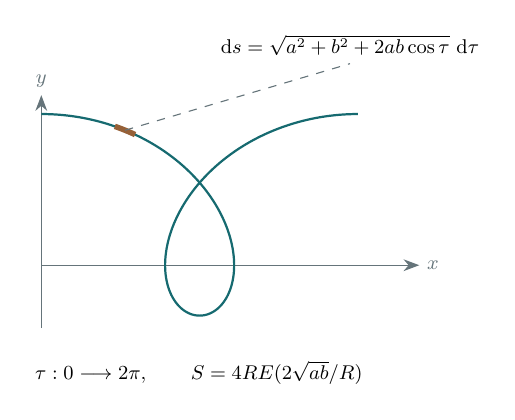
\begin{tikzpicture}[scale=.8,transform shape]
\draw[axis] (0,0)--(6,0) node[right] {$x$};
\draw[axis] (0,-1)--(0,2.7) node[above] {$y$};
\draw[traj] plot coordinates {(0.00000000,2.40000000) (0.06282707,2.39945172) (0.12562543,2.39780726) (0.18836641,2.39506773) (0.25102135,2.39123503) (0.31356166,2.38631178) (0.37595885,2.38030134) (0.43818450,2.37320785) (0.50021031,2.36503616) (0.56200814,2.35579187) (0.62354998,2.34548132) (0.68480801,2.33411158) (0.74575460,2.32169043) (0.80636234,2.30822639) (0.86660403,2.29372868) (0.92645276,2.27820725) (0.98588185,2.26167273) (1.04486492,2.24413645) (1.10337592,2.22561044) (1.16138909,2.20610738) (1.21887902,2.18564065) (1.27582068,2.16422426) (1.33218938,2.14187291) (1.38796085,2.11860190) (1.44311123,2.09442719) (1.49761706,2.06936534) (1.55145535,2.04343354) (1.60460355,2.01664954) (1.65703960,1.98903172) (1.70874190,1.96059899) (1.75968938,1.93137085) (1.80986148,1.90136732) (1.85923815,1.87060897) (1.90779993,1.83911688) (1.95552787,1.80691263) (2.00240363,1.77401829) (2.04840943,1.74045640) (2.09352809,1.70624998) (2.13774305,1.67142246) (2.18103835,1.63599770) (2.22339869,1.60000000) (2.26480937,1.56345402) (2.30525638,1.52638480) (2.34472635,1.48881775) (2.38320658,1.45077863) (2.42068505,1.41229349) (2.45715043,1.37338872) (2.49259208,1.33409097) (2.52700008,1.29442719) (2.56036518,1.25442455) (2.59267887,1.21411047) (2.62393337,1.17351258) (2.65412161,1.13265871) (2.68323726,1.09157684) (2.71127470,1.05029514) (2.73822908,1.00884191) (2.76409629,0.96724554) (2.78887294,0.92553455) (2.81255641,0.88373753) (2.83514483,0.84188312) (2.85663706,0.80000000) (2.87703273,0.75811688) (2.89633222,0.71626247) (2.91453665,0.67446545) (2.93164790,0.63275446) (2.94766859,0.59115809) (2.96260211,0.54970486) (2.97645257,0.50842316) (2.98922483,0.46734129) (3.00092449,0.42648742) (3.01155789,0.38588953) (3.02113210,0.34557545) (3.02965490,0.30557281) (3.03713481,0.26590903) (3.04358106,0.22661128) (3.04900358,0.18770651) (3.05341301,0.14922137) (3.05682068,0.11118225) (3.05923862,0.07361520) (3.06067951,0.03654598) (3.06115673,0.00000000) (3.06068430,-0.03599770) (3.05927689,-0.07142246) (3.05694984,-0.10624998) (3.05371908,-0.14045640) (3.04960118,-0.17401829) (3.04461333,-0.20691263) (3.03877328,-0.23911688) (3.03209941,-0.27060897) (3.02461063,-0.30136732) (3.01632644,-0.33137085) (3.00726686,-0.36059899) (2.99745246,-0.38903172) (2.98690432,-0.41664954) (2.97564402,-0.44343354) (2.96369363,-0.46936534) (2.95107570,-0.49442719) (2.93781323,-0.51860190) (2.92392966,-0.54187291) (2.90944885,-0.56422426) (2.89439510,-0.58564065) (2.87879307,-0.60610738) (2.86266780,-0.62561044) (2.84604471,-0.64413645) (2.82894954,-0.66167273) (2.81140835,-0.67820725) (2.79344753,-0.69372868) (2.77509373,-0.70822639) (2.75637390,-0.72169043) (2.73731521,-0.73411158) (2.71794508,-0.74548132) (2.69829115,-0.75579187) (2.67838122,-0.76503616) (2.65824331,-0.77320785) (2.63790556,-0.78030134) (2.61739628,-0.78631178) (2.59674386,-0.79123503) (2.57597682,-0.79506773) (2.55512375,-0.79780726) (2.53421329,-0.79945172) (2.51327412,-0.80000000) (2.49233496,-0.79945172) (2.47142449,-0.79780726) (2.45057142,-0.79506773) (2.42980439,-0.79123503) (2.40915197,-0.78631178) (2.38864268,-0.78030134) (2.36830494,-0.77320785) (2.34816703,-0.76503616) (2.32825710,-0.75579187) (2.30860316,-0.74548132) (2.28923303,-0.73411158) (2.27017434,-0.72169043) (2.25145451,-0.70822639) (2.23310072,-0.69372868) (2.21513990,-0.67820725) (2.19759871,-0.66167273) (2.18050354,-0.64413645) (2.16388044,-0.62561044) (2.14775518,-0.60610738) (2.13215314,-0.58564065) (2.11709939,-0.56422426) (2.10261859,-0.54187291) (2.08873502,-0.51860190) (2.07547254,-0.49442719) (2.06285461,-0.46936534) (2.05090422,-0.44343354) (2.03964392,-0.41664954) (2.02909578,-0.38903172) (2.01928138,-0.36059899) (2.01022180,-0.33137085) (2.00193761,-0.30136732) (1.99444883,-0.27060897) (1.98777496,-0.23911688) (1.98193492,-0.20691263) (1.97694706,-0.17401829) (1.97282917,-0.14045640) (1.96959841,-0.10624998) (1.96727135,-0.07142246) (1.96586395,-0.03599770) (1.96539152,-0.00000000) (1.96586873,0.03654598) (1.96730963,0.07361520) (1.96972756,0.11118225) (1.97313524,0.14922137) (1.97754467,0.18770651) (1.98296719,0.22661128) (1.98941344,0.26590903) (1.99689335,0.30557281) (2.00541615,0.34557545) (2.01499035,0.38588953) (2.02562375,0.42648742) (2.03732341,0.46734129) (2.05009568,0.50842316) (2.06394613,0.54970486) (2.07887965,0.59115809) (2.09490035,0.63275446) (2.11201160,0.67446545) (2.13021603,0.71626247) (2.14951551,0.75811688) (2.16991118,0.80000000) (2.19140342,0.84188312) (2.21399183,0.88373753) (2.23767530,0.92553455) (2.26245196,0.96724554) (2.28831916,1.00884191) (2.31527355,1.05029514) (2.34331099,1.09157684) (2.37242663,1.13265871) (2.40261487,1.17351258) (2.43386937,1.21411047) (2.46618307,1.25442455) (2.49954817,1.29442719) (2.53395616,1.33409097) (2.56939782,1.37338872) (2.60586320,1.41229349) (2.64334167,1.45077863) (2.68182190,1.48881775) (2.72129186,1.52638480) (2.76173887,1.56345402) (2.80314956,1.60000000) (2.84550989,1.63599770) (2.88880520,1.67142246) (2.93302016,1.70624998) (2.97813882,1.74045640) (3.02414462,1.77401829) (3.07102037,1.80691263) (3.11874832,1.83911688) (3.16731009,1.87060897) (3.21668677,1.90136732) (3.26685887,1.93137085) (3.31780634,1.96059899) (3.36950865,1.98903172) (3.42194469,2.01664954) (3.47509289,2.04343354) (3.52893118,2.06936534) (3.58343702,2.09442719) (3.63858739,2.11860190) (3.69435887,2.14187291) (3.75072757,2.16422426) (3.80766923,2.18564065) (3.86515916,2.20610738) (3.92317233,2.22561044) (3.98168332,2.24413645) (4.04066640,2.26167273) (4.10009549,2.27820725) (4.15994421,2.29372868) (4.22018591,2.30822639) (4.28079364,2.32169043) (4.34174023,2.33411158) (4.40299826,2.34548132) (4.46454010,2.35579187) (4.52633793,2.36503616) (4.58836375,2.37320785) (4.65058940,2.38030134) (4.71298658,2.38631178) (4.77552690,2.39123503) (4.83818184,2.39506773) (4.90092281,2.39780726) (4.96372118,2.39945172) (5.02654825,2.40000000)};
\draw[line width=2pt,color=warm] plot coordinates {(1.16708086,2.20413210) (1.18359018,2.19833956) (1.20005576,2.19246836) (1.21647701,2.18651883) (1.23285335,2.18049131) (1.24918418,2.17438614) (1.26546894,2.16820367) (1.28170705,2.16194423) (1.29789792,2.15560818) (1.31404098,2.14919588) (1.33013567,2.14270768) (1.34618141,2.13614396) (1.36217764,2.12950509) (1.37812380,2.12279142) (1.39401932,2.11600336) (1.40986366,2.10914126) (1.42565626,2.10220553) (1.44139656,2.09519655) (1.45708402,2.08811471) (1.47271810,2.08096042) (1.48829825,2.07373408)};
\draw[guide] (1.33013567,2.14270768)--(4.9,3.2);
\node[above] at (4.9,3.2) {$\dd s=\sqrt{a^2+b^2+2ab\cos\tau}\,\dd\tau$};
\node[below] at (2.5,-1.4) {$\tau:0\longrightarrow2\pi,\qquad S=4R E(2\sqrt{ab}/R)$};
\end{tikzpicture}
\figcaption{变图力试2.1V7\quad 完整弧长积分连接圆轨道极限和尖点摆线极限}
\end{minipage}\end{center}

\Needspace{20\baselineskip}
\item 取$M/m\to\infty$，求轨道、支持力、周期和三类曲率的极限。
\textbf{解：}变图力试2.1V8中$b,V_C\to0$、$a\to R$，环心运动幅度和加速度都趋零。质点方程回到$x=R\sin\omega t,y=R\cos\omega t$，周期$2\pi R/v_0$，支持力趋于$mv_0^2/R$。三类曲率半径均趋于$R$，竖直切线位于$\tau=\pi/2,3\pi/2$。固定大质量圆环的圆周运动由同一两体解连续得到。
\begin{center}\begin{minipage}{.98\linewidth}\centering
\begin{tikzpicture}[scale=.8,transform shape]
\draw[object] (0,0) circle(2);\fill (0,2) circle(.04) node[above] {$m$};\fill (0,0) circle(.04) node[below] {近似固定环心};\draw[motion] (0,2)--(1.5,2) node[right] {$v_0$};\node at (5,1) {$M/m\to\infty$};\node at (5,-.5) {$\rho_1,\rho_2,\rho_3\to R$};
\end{tikzpicture}
\figcaption{变图力试2.1V8\quad 大质量圆环极限回到固定圆内的匀速圆周运动}
\end{minipage}\end{center}
\end{enumerate}

\Needspace{13\baselineskip}

\pdfbookmark[2]{第 2 题 三次喷气中的能量、速度矢量与落地点}{q2}

\section*{第 2 题\quad 三次喷气中的能量、速度矢量与落地点}\label{q:2}


飞船起初在半径$r_0$的圆轨道上绕地球运动。每次喷气持续时间极短，喷气过程中位置不变，各阶段把飞船质量视为常量。将单位质量的冲量$\Delta\boldsymbol v=\Delta\boldsymbol p/m$称为比冲量，其大小单位为速度。地球质量为$M_E$、半径为$R_E$，$r_1>r_0>R_E$，忽略空气阻力。
\begin{enumerate}
\item 第一次喷气使飞船刚能逃逸，求最小比冲量及排气方向。
\item 第一次取上述最小值。飞船沿上升轨迹到达$r_1$处，第二次喷气使它进入半径$r_1$的同向圆轨道。求比冲量及排气方向。
\item 飞船在该圆轨道的$A$点第三次喷气，希望在对径方向的地表点$B$与地表相切。分别讨论向正前方排气和沿径向向外排气；检查两者是否都能到达指定的$B$。若只要求在某地表点相切而不限定方位，求两种比冲量，并在$r_0=2R_E$时比较。
\end{enumerate}
各次排气方向指相对飞船的喷气方向，与飞船获得的冲量方向相反。“与地表相切”指飞船到地表时的瞬时速度沿当地切线，落地速率由轨道确定。


\begin{center}\begin{minipage}{.98\linewidth}\centering
\begin{tikzpicture}[scale=.9,transform shape]
\draw[object] (0.00000,0.00000) circle(1.00000);\draw[guide] (0.00000,0.00000) circle(2.00000);\draw[guide] (0.00000,0.00000) circle(4.00000);\fill (0.00000,0.00000) circle(.035);\node[below] at (0.00000,0.00000) {$O$};\fill (4.00000,0.00000) circle(.035);\node[right] at (4.00000,0.00000) {$A$};\fill (-1.00000,0.00000) circle(.035);\node[left] at (-1.00000,0.00000) {$B$};\draw[guide] (-1.00000,0.00000)--(4.00000,0.00000);\node[above] at (0.00000,1.00000) {$R_E$};\node[above left] at (-2.40000,0.40000) {$r_0$};\node[above] at (0.00000,4.00000) {$r_1$};\draw[motion] (-2.00000,0.00000)--(-2.00000,-1.30000);\node[left] at (-2.10000,-1.00000) {$v_0$};
\end{tikzpicture}
\figcaption{图力试2.2\quad 三条同心尺度及第三次喷气的指定对径地表点B。}
\end{minipage}\end{center}

\Needspace{8\baselineskip}

\pdfbookmark[3]{题型定位}{q2-h0}

\subsection*{题型定位}

三次瞬时冲量依次确定逃逸轨道、目标圆轨道和接地轨道。喷气间使用中心引力的能量及角动量守恒，喷气瞬间按目标速度减去当前速度求比冲量。第三问还要求指定地表方位，轨道偏心率矢量将这一位置条件与能量、角动量同时联系起来。

\Needspace{8\baselineskip}

\pdfbookmark[3]{知识点}{q2-h1}

\subsection*{知识点}

圆轨道速度与逃逸速度分别由向心条件和零机械能确定。最小逃逸冲量与初速同向，排气反向。抛物线在给定半径处同时具有径向、切向速度，入圆时径向分量归零、切向分量调到圆速。中心轨道的能量、角动量及偏心率矢量共同给轨道尺度、类型和近地点方位。

\Needspace{8\baselineskip}

\pdfbookmark[3]{物理图像}{q2-h2}

\subsection*{物理图像}

解图力试2.2A画入圆前后速度矢量及其差，反向箭头给排气方向。图B的切向方案从椭圆远地点到对径近地点。图C的纯径向方案将近地点放在$B_r$，相对$A$方位差为90度，指定对径点$B$位于另一方向。图D比较放宽落点条件后两种比冲量，始终保留相切点的差别。

\Needspace{8\baselineskip}

\pdfbookmark[3]{解题入口}{q2-h3}

\subsection*{解题入口}

第一冲取最小逃逸值，确定后续为零能量抛物线。第二冲先列当前$v_r,v_t$与目标圆速，再作矢量差。第三冲先求切向方案的两拱点速度，再求纯径向冲量对应的偏心率矢量，标出近地点方位。比较冲量时明确是在固定对径落点还是放宽落点的任务下。

\Needspace{8\baselineskip}

\pdfbookmark[3]{标准解法}{q2-h4}

\subsection*{标准解法}


图力试2.2取地心为$O$。令$\mu=GM_E$，轨道速度在当地径向$\hat r$和沿运动切向$\hat t$中分解。喷气阶段可改变机械能与角动量；两次喷气之间只受中心引力，这两个量才守恒。

圆轨道的向心条件为$m v_0^2/r_0=\mu m/r_0^2$，飞船质量约去后确定初始圆速。第一次喷气的目标速率再由单位质量总能量为零确定，两个速度条件对应不同轨道。
（1）初始圆轨道速度为$v_0=\sqrt{\mu/r_0}$。刚能逃逸要求喷气后单位质量机械能为零：
\[
\frac{v_{e0}^2}{2}-\frac{\mu}{r_0}=0,\qquad
v_{e0}=\sqrt{\frac{2\mu}{r_0}}.
\]
在给定速度大小$v_{e0}$时，与初始速度同向的速度改变量最小，由速度矢量三角不等式得
\[
\boxed{\Delta v_0=v_{e0}-v_0
=(\sqrt2-1)\sqrt{\frac{\mu}{r_0}}}.
\]
飞船加速方向沿$\hat t$，所以气体向后喷出。随后飞船沿近地点半径$r_0$的抛物线向外运动。

\begin{center}\begin{minipage}{.98\linewidth}\centering
\begin{tikzpicture}[scale=.82,transform shape]
\draw[axis] (0.00000,0.00000)--(4.45000,0.00000);\draw[axis] (0.00000,0.00000)--(0.00000,3.65000);\node[below right] at (4.45000,0.00000) {$\hat r$};\node[above right] at (0.00000,3.65000) {$\hat t$};\draw[motion] (0.00000,0.00000)--(2.82843,2.00000);\node[above right] at (2.82843,2.00000) {$\boldsymbol v_e$};\draw[force] (0.00000,0.00000)--(0.00000,2.44949);\node[left] at (-0.10000,1.50000) {$v_c$};\draw[force] (2.82843,2.00000)--(0.00000,2.44949);\node[above] at (1.20000,2.80000) {$\Delta\boldsymbol v_1$};\draw[guide] (2.82843,2.00000)--(2.82843,0.00000);\node[below] at (1.41421,-0.10000) {$v_r$};\node[right] at (2.92843,1.00000) {$v_t$};\draw[motion] (5.00000,2.00000)--(6.60000,1.75000);\node[above] at (5.80000,2.10000) {排气 $-\Delta\boldsymbol v_1$};\node[above] at (3.20000,4.20000) {示例 $r_1=3r_0>2r_0$};\node[below] at (3.00000,-1.20000) {先消径向分量，再调切向分量};
\end{tikzpicture}
\figcaption{解图力试2.2A\quad 第二冲是速度矢量差，排气方向与它相反。}
\end{minipage}\end{center}
（2）解图力试2.2A在第二次喷气点画出此前的径向和切向速度。抛物线单位质量能量为零，角动量$j=\sqrt{2\mu r_0}$。在$r_1$处，
\[
v_e^2=\frac{2\mu}{r_1},\qquad
v_t=\frac{j}{r_1}=\frac{\sqrt{2\mu r_0}}{r_1},
\]
\[
v_r=\sqrt{v_e^2-v_t^2}
=\frac{\sqrt{2\mu(r_1-r_0)}}{r_1}>0.
\]
目标圆轨道速度为$v_c=\sqrt{\mu/r_1}$，只有切向分量。因此飞船所需比冲量矢量为
\[
\boxed{\Delta\boldsymbol v_1=-v_r\hat r+(v_c-v_t)\hat t},
\]
\[
\boxed{\Delta v_1
=\sqrt{\frac{\mu}{r_1}
\left(3-2\sqrt{\frac{2r_0}{r_1}}\right)}}.
\]
排气沿反方向$v_r\hat r+(v_t-v_c)\hat t$。其径向分量始终向外，而切向分量在$r_1=2r_0$变号：$r_1<2r_0$时沿前方，$r_1>2r_0$时沿后方，等号时纯径向向外。径向分量和切向分量一起确定入圆冲量与排气方向。

若将喷气前速度与圆轨道切向的夹角记为$\phi$，则$\cos\phi=v_t/v_e=\sqrt{r_0/r_1}$。速度三角形也给$\Delta v_1^2=v_e^2+v_c^2-2v_ev_c\cos\phi$，其中径向部分已由完整夹角计入。比较排气方向时，下面的点积式又可写成余弦定理形式$\cos\alpha=(v_e^2+\Delta v_1^2-v_c^2)/(2v_e\Delta v_1)$，两种表达使用同一组速度矢量。
若以$\alpha$表示排气与喷气前飞船速度的夹角，由点积可得
\[
\cos\alpha=
\frac{v_r^2+(v_t-v_c)v_t}{v_e\Delta v_1}
=\frac{2-\sqrt{2r_0/r_1}}
{\sqrt{2(3-2\sqrt{2r_0/r_1})}}.
\]

\begin{center}\begin{minipage}{.98\linewidth}\centering
\begin{tikzpicture}[scale=.83,transform shape]
\draw[object] (0.00000,0.00000) circle(1.00000);\node[anchor=center] at (0.00000,0.00000) {$O$};\draw[traj] plot coordinates {(4.00000,0.00000) (3.99897,0.05737) (3.99589,0.11470) (3.99075,0.17193) (3.98356,0.22902) (3.97432,0.28592) (3.96305,0.34259) (3.94975,0.39897) (3.93444,0.45503) (3.91712,0.51071) (3.89781,0.56597) (3.87653,0.62076) (3.85329,0.67505) (3.82812,0.72877) (3.80103,0.78190) (3.77204,0.83439) (3.74119,0.88619) (3.70849,0.93725) (3.67397,0.98755) (3.63767,1.03704) (3.59960,1.08567) (3.55981,1.13340) (3.51832,1.18021) (3.47517,1.22604) (3.43039,1.27086) (3.38403,1.31464) (3.33611,1.35734) (3.28668,1.39892) (3.23579,1.43934) (3.18346,1.47859) (3.12975,1.51661) (3.07469,1.55339) (3.01834,1.58889) (2.96075,1.62308) (2.90194,1.65593) (2.84199,1.68742) (2.78093,1.71753) (2.71881,1.74622) (2.65570,1.77347) (2.59163,1.79926) (2.52666,1.82357) (2.46085,1.84638) (2.39425,1.86767) (2.32691,1.88743) (2.25889,1.90563) (2.19024,1.92226) (2.12103,1.93731) (2.05131,1.95076) (1.98113,1.96261) (1.91056,1.97285) (1.83964,1.98146) (1.76845,1.98844) (1.69704,1.99378) (1.62547,1.99748) (1.55379,1.99954) (1.48207,1.99995) (1.41036,1.99871) (1.33873,1.99583) (1.26723,1.99131) (1.19592,1.98515) (1.12486,1.97736) (1.05411,1.96793) (0.98373,1.95689) (0.91377,1.94424) (0.84430,1.92998) (0.77536,1.91414) (0.70702,1.89672) (0.63934,1.87774) (0.57236,1.85722) (0.50614,1.83517) (0.44075,1.81160) (0.37622,1.78655) (0.31262,1.76002) (0.25000,1.73205) (0.18841,1.70265) (0.12789,1.67185) (0.06851,1.63967) (0.01030,1.60615) (-0.04668,1.57130) (-0.10239,1.53516) (-0.15677,1.49775) (-0.20980,1.45912) (-0.26142,1.41928) (-0.31158,1.37827) (-0.36026,1.33613) (-0.40741,1.29289) (-0.45298,1.24858) (-0.49695,1.20325) (-0.53927,1.15692) (-0.57992,1.10965) (-0.61885,1.06146) (-0.65604,1.01240) (-0.69146,0.96250) (-0.72507,0.91181) (-0.75685,0.86037) (-0.78677,0.80823) (-0.81481,0.75542) (-0.84095,0.70198) (-0.86516,0.64797) (-0.88742,0.59343) (-0.90771,0.53839) (-0.92603,0.48292) (-0.94235,0.42704) (-0.95665,0.37082) (-0.96894,0.31429) (-0.97919,0.25750) (-0.98741,0.20050) (-0.99357,0.14333) (-0.99769,0.08604) (-0.99974,0.02869) (-0.99974,-0.02869) (-0.99769,-0.08604) (-0.99357,-0.14333) (-0.98741,-0.20050) (-0.97919,-0.25750) (-0.96894,-0.31429) (-0.95665,-0.37082) (-0.94235,-0.42704) (-0.92603,-0.48292) (-0.90771,-0.53839) (-0.88742,-0.59343) (-0.86516,-0.64797) (-0.84095,-0.70198) (-0.81481,-0.75542) (-0.78677,-0.80823) (-0.75685,-0.86037) (-0.72507,-0.91181) (-0.69146,-0.96250) (-0.65604,-1.01240) (-0.61885,-1.06146) (-0.57992,-1.10965) (-0.53927,-1.15692) (-0.49695,-1.20325) (-0.45298,-1.24858) (-0.40741,-1.29289) (-0.36026,-1.33613) (-0.31158,-1.37827) (-0.26142,-1.41928) (-0.20980,-1.45912) (-0.15677,-1.49775) (-0.10239,-1.53516) (-0.04668,-1.57130) (0.01030,-1.60615) (0.06851,-1.63967) (0.12789,-1.67185) (0.18841,-1.70265) (0.25000,-1.73205) (0.31262,-1.76002) (0.37622,-1.78655) (0.44075,-1.81160) (0.50614,-1.83517) (0.57236,-1.85722) (0.63934,-1.87774) (0.70702,-1.89672) (0.77536,-1.91414) (0.84430,-1.92998) (0.91377,-1.94424) (0.98373,-1.95689) (1.05411,-1.96793) (1.12486,-1.97736) (1.19592,-1.98515) (1.26723,-1.99131) (1.33873,-1.99583) (1.41036,-1.99871) (1.48207,-1.99995) (1.55379,-1.99954) (1.62547,-1.99748) (1.69704,-1.99378) (1.76845,-1.98844) (1.83964,-1.98146) (1.91056,-1.97285) (1.98113,-1.96261) (2.05131,-1.95076) (2.12103,-1.93731) (2.19024,-1.92226) (2.25889,-1.90563) (2.32691,-1.88743) (2.39425,-1.86767) (2.46085,-1.84638) (2.52666,-1.82357) (2.59163,-1.79926) (2.65570,-1.77347) (2.71881,-1.74622) (2.78093,-1.71753) (2.84199,-1.68742) (2.90194,-1.65593) (2.96075,-1.62308) (3.01834,-1.58889) (3.07469,-1.55339) (3.12975,-1.51661) (3.18346,-1.47859) (3.23579,-1.43934) (3.28668,-1.39892) (3.33611,-1.35734) (3.38403,-1.31464) (3.43039,-1.27086) (3.47517,-1.22604) (3.51832,-1.18021) (3.55981,-1.13340) (3.59960,-1.08567) (3.63767,-1.03704) (3.67397,-0.98755) (3.70849,-0.93725) (3.74119,-0.88619) (3.77204,-0.83439) (3.80103,-0.78190) (3.82812,-0.72877) (3.85329,-0.67505) (3.87653,-0.62076) (3.89781,-0.56597) (3.91712,-0.51071) (3.93444,-0.45503) (3.94975,-0.39897) (3.96305,-0.34259) (3.97432,-0.28592) (3.98356,-0.22902) (3.99075,-0.17193) (3.99589,-0.11470) (3.99897,-0.05737) (4.00000,-0.00000)};\fill (4.00000,0.00000) circle(.035);\node[below right] at (4.00000,0.00000) {$A$};\fill (-1.00000,0.00000) circle(.035);\node[left] at (-1.00000,0.00000) {$B$};\draw[guide] (-1.00000,0.00000)--(4.00000,0.00000);\draw[motion] (4.00000,0.00000)--(4.00000,1.10000);\node[above left] at (4.00000,1.10000) {$v_a$};\draw[force] (4.60000,0.00000)--(4.60000,1.70000);\node[right] at (4.80000,1.70000) {前向排气};\draw[motion] (-1.00000,0.00000)--(-1.00000,-1.50000);\node[below left] at (-1.00000,-1.50000) {$v_p$};\node[above] at (1.50000,3.00000) {A远地点，B近地点，方位差 $\pi$};\draw[<->,thin,color=muted] (0.00000,-3.00000)--(4.00000,-3.00000);\node[below] at (2.00000,-3.00000) {$r_1$};\draw[<->,thin,color=muted] (-1.00000,-4.00000)--(0.00000,-4.00000);\node[below] at (-0.50000,-4.00000) {$R_E$};
\end{tikzpicture}
\figcaption{解图力试2.2B\quad 切向减速产生对径拱点，能到达指定B。}
\end{minipage}\end{center}
（3）解图力试2.2B的切向方案向前排气，飞船切向减速。欲从$A$到对径地表点$B$并相切，$A$为椭圆远地点、$B$为近地点。设减速后速率为$v_a$、到$B$时为$v_p$，则
\[
r_1v_a=R_Ev_p,\qquad
\frac{v_a^2}{2}-\frac{\mu}{r_1}
=\frac{v_p^2}{2}-\frac{\mu}{R_E}.
\]
由角动量式先取$v_p=(r_1/R_E)v_a$，代入能量式有$v_a^2[(r_1/R_E)^2-1]=2\mu(1/R_E-1/r_1)$。两边含有的$r_1-R_E$因子约去后得到远地点速率，取正根对应仍沿原方向运动的返回支。
消去$v_p$，
\[
v_a^2=\frac{2\mu R_E}{r_1(r_1+R_E)},\qquad
\boxed{\Delta v_t=v_c-v_a
=v_c\left(1-\sqrt{\frac{2R_E}{r_1+R_E}}\right)}.
\]
该椭圆的两拱点确在同一直径两侧，符合指定落地点。

\begin{center}\begin{minipage}{.98\linewidth}\centering
\begin{tikzpicture}[scale=.83,transform shape]
\draw[object] (0.00000,0.00000) circle(1.00000);\node[below right] at (0.00000,-0.30000) {$O$};\draw[traj] plot coordinates {(3.00000,0.00000) (2.92290,0.03842) (2.84917,0.07492) (2.77858,0.10963) (2.71091,0.14267) (2.64597,0.17415) (2.58357,0.20419) (2.52356,0.23286) (2.46579,0.26026) (2.41011,0.28646) (2.35641,0.31154) (2.30457,0.33556) (2.25447,0.35859) (2.20603,0.38068) (2.15914,0.40189) (2.11373,0.42225) (2.06971,0.44183) (2.02701,0.46065) (1.98557,0.47876) (1.94531,0.49620) (1.90618,0.51300) (1.86812,0.52919) (1.83109,0.54479) (1.79502,0.55985) (1.75988,0.57438) (1.72563,0.58841) (1.69221,0.60196) (1.65960,0.61505) (1.62776,0.62770) (1.59665,0.63994) (1.56624,0.65178) (1.53651,0.66323) (1.50742,0.67432) (1.47895,0.68505) (1.45107,0.69544) (1.42376,0.70551) (1.39699,0.71527) (1.37074,0.72473) (1.34500,0.73390) (1.31973,0.74279) (1.29494,0.75142) (1.27058,0.75979) (1.24666,0.76791) (1.22315,0.77579) (1.20004,0.78343) (1.17731,0.79086) (1.15495,0.79807) (1.13295,0.80507) (1.11129,0.81187) (1.08996,0.81847) (1.06895,0.82489) (1.04824,0.83112) (1.02783,0.83718) (1.00771,0.84307) (0.98787,0.84879) (0.96829,0.85434) (0.94897,0.85974) (0.92990,0.86499) (0.91107,0.87009) (0.89248,0.87505) (0.87411,0.87987) (0.85595,0.88455) (0.83801,0.88911) (0.82027,0.89353) (0.80272,0.89783) (0.78537,0.90200) (0.76820,0.90606) (0.75121,0.91000) (0.73438,0.91383) (0.71773,0.91754) (0.70123,0.92115) (0.68489,0.92466) (0.66870,0.92806) (0.65265,0.93136) (0.63675,0.93457) (0.62098,0.93767) (0.60534,0.94069) (0.58982,0.94361) (0.57443,0.94644) (0.55916,0.94918) (0.54400,0.95184) (0.52895,0.95441) (0.51400,0.95690) (0.49916,0.95930) (0.48441,0.96163) (0.46976,0.96387) (0.45521,0.96604) (0.44073,0.96813) (0.42635,0.97015) (0.41204,0.97209) (0.39782,0.97396) (0.38366,0.97576) (0.36958,0.97749) (0.35557,0.97915) (0.34162,0.98073) (0.32774,0.98226) (0.31392,0.98371) (0.30015,0.98510) (0.28644,0.98642) (0.27278,0.98767) (0.25917,0.98887) (0.24561,0.99000) (0.23209,0.99106) (0.21861,0.99207) (0.20517,0.99301) (0.19176,0.99389) (0.17839,0.99471) (0.16505,0.99547) (0.15174,0.99617) (0.13846,0.99681) (0.12520,0.99739) (0.11196,0.99791) (0.09875,0.99838) (0.08554,0.99878) (0.07236,0.99913) (0.05919,0.99942) (0.04602,0.99965) (0.03287,0.99982) (0.01972,0.99994) (0.00657,0.99999) (-0.00657,0.99999) (-0.01972,0.99994) (-0.03287,0.99982) (-0.04602,0.99965) (-0.05919,0.99942) (-0.07236,0.99913) (-0.08554,0.99878) (-0.09875,0.99838) (-0.11196,0.99791) (-0.12520,0.99739) (-0.13846,0.99681) (-0.15174,0.99617) (-0.16505,0.99547) (-0.17839,0.99471) (-0.19176,0.99389) (-0.20517,0.99301) (-0.21861,0.99207) (-0.23209,0.99106) (-0.24561,0.99000) (-0.25917,0.98887) (-0.27278,0.98767) (-0.28644,0.98642) (-0.30015,0.98510) (-0.31392,0.98371) (-0.32774,0.98226) (-0.34162,0.98073) (-0.35557,0.97915) (-0.36958,0.97749) (-0.38366,0.97576) (-0.39782,0.97396) (-0.41204,0.97209) (-0.42635,0.97015) (-0.44073,0.96813) (-0.45521,0.96604) (-0.46976,0.96387) (-0.48441,0.96163) (-0.49916,0.95930) (-0.51400,0.95690) (-0.52895,0.95441) (-0.54400,0.95184) (-0.55916,0.94918) (-0.57443,0.94644) (-0.58982,0.94361) (-0.60534,0.94069) (-0.62098,0.93767) (-0.63675,0.93457) (-0.65265,0.93136) (-0.66870,0.92806) (-0.68489,0.92466) (-0.70123,0.92115) (-0.71773,0.91754) (-0.73438,0.91383) (-0.75121,0.91000) (-0.76820,0.90606) (-0.78537,0.90200) (-0.80272,0.89783) (-0.82027,0.89353) (-0.83801,0.88911) (-0.85595,0.88455) (-0.87411,0.87987) (-0.89248,0.87505) (-0.91107,0.87009) (-0.92990,0.86499) (-0.94897,0.85974) (-0.96829,0.85434) (-0.98787,0.84879) (-1.00771,0.84307) (-1.02783,0.83718) (-1.04824,0.83112) (-1.06895,0.82489) (-1.08996,0.81847) (-1.11129,0.81187) (-1.13295,0.80507) (-1.15495,0.79807) (-1.17731,0.79086) (-1.20004,0.78343) (-1.22315,0.77579) (-1.24666,0.76791) (-1.27058,0.75979) (-1.29494,0.75142) (-1.31973,0.74279) (-1.34500,0.73390) (-1.37074,0.72473) (-1.39699,0.71527) (-1.42376,0.70551) (-1.45107,0.69544) (-1.47895,0.68505) (-1.50742,0.67432) (-1.53651,0.66323) (-1.56624,0.65178) (-1.59665,0.63994) (-1.62776,0.62770) (-1.65960,0.61505) (-1.69221,0.60196) (-1.72563,0.58841) (-1.75988,0.57438) (-1.79502,0.55985) (-1.83109,0.54479) (-1.86812,0.52919) (-1.90618,0.51300) (-1.94531,0.49620) (-1.98557,0.47876) (-2.02701,0.46065) (-2.06971,0.44183) (-2.11373,0.42225) (-2.15914,0.40189) (-2.20603,0.38068) (-2.25447,0.35859) (-2.30457,0.33556) (-2.35641,0.31154) (-2.41011,0.28646) (-2.46579,0.26026) (-2.52356,0.23286) (-2.58357,0.20419) (-2.64597,0.17415) (-2.71091,0.14267) (-2.77858,0.10963) (-2.84917,0.07492) (-2.92290,0.03842) (-3.00000,0.00000)};\fill (3.00000,0.00000) circle(.035);\node[below right] at (3.00000,0.00000) {$A$};\fill (0.00000,1.00000) circle(.035);\node[above] at (0.00000,1.00000) {$B_r$相切};\fill (-1.00000,0.00000) circle(.035);\node[below left] at (-1.00000,0.00000) {指定 $B$};\fill (-3.00000,0.00000) circle(.035);\node[below left] at (-3.00000,0.00000) {$r(\pi)=r_1$};\draw[guide] (-3.40000,0.00000)--(4.80000,0.00000);\draw[force] (3.00000,0.00000)--(1.40000,0.80000);\node[above right] at (1.40000,0.80000) {$-u\hat r+v_c\hat t$};\draw[motion] (3.00000,-0.60000)--(4.60000,-0.60000);\node[below] at (4.00000,-0.70000) {径向向外排气};\node[above] at (0.00000,2.60000) {示例 $r_1=3R_E$：双曲线先向内运行};\node[below] at (0.00000,-2.30000) {相切点在90°方位，对径方位处半径仍为$r_1$};
\end{tikzpicture}
\figcaption{解图力试2.2C\quad 纯径向冲量的近地点在Br，与指定B方位不同。}
\end{minipage}\end{center}
解图力试2.2C的径向排气给飞船一个向内比冲量$u$，切向速度仍为$v_c$，单位质量角动量仍为$j=r_1v_c$。若暂时只要求在某地表点$B_r$相切，能量与角动量给
\[
\frac{v_c^2+u^2}{2}-\frac{\mu}{r_1}
=\frac{(r_1v_c/R_E)^2}{2}-\frac{\mu}{R_E},
\]
\[
\boxed{u=\Delta v_r=v_c\left(\frac{r_1}{R_E}-1\right)}.
\]
接着由同一喷后速度求近地点方位，将接地半径与指定位置一起确定。把$A$放在$+x$轴，取初始切向速度向$+y$，径向喷气后的速度是$-u\hat x+v_c\hat y$。这里$\boldsymbol j=r_1v_c\hat z$，因此$\boldsymbol v\times\boldsymbol j=r_1v_c^2\hat x+r_1uv_c\hat y$。第一项除以$\mu$恰为$\hat x$，与偏心率定义中的径向单位矢量抵消，余下分量确定真正的近地点方向。
它的轨道偏心率矢量为
\[
\boldsymbol e=\frac{\boldsymbol v\times\boldsymbol j}{\mu}-\hat r
=\frac{u}{v_c}\hat y.
\]
近地点沿$+y$，离$A$的方位差为$\pi/2$，不是对径的$\pi$。轨道方程也直接说明：
\[
r(\phi)=\frac{r_1}{1+(u/v_c)\sin\phi},
\qquad r(\pi)=r_1>R_E.
\]
所以\textbf{纯径向方案的近地点在$B_r$，对径方位处的轨道半径为$r_1>R_E$}。上面的$\Delta v_r$只能回答放宽落地点后的相切问题；该轨道满足接地半径，近地点方位则由偏心率矢量指向$B_r$。

对于放宽的任务，令$q=r_1/R_E>1$，则轨道偏心率$e=q-1$。当$1<q<2$时为椭圆，$q=2$时为抛物线，$q>2$时为先向内接近地球的双曲线。若$r_0=2R_E$且$r_1>r_0$，径向返回段实际属于双曲线。

最后比较两种放宽方案的比冲量：
\[
\frac{\Delta v_r-\Delta v_t}{v_c}
=q-2+\sqrt{\frac2{q+1}}>0,\qquad q>1.
\]
右式在$q=1$为零，导数为$1-\tfrac1{\sqrt2}(q+1)^{-3/2}>0$，因此
\[
\boxed{\Delta v_r>\Delta v_t}.
\]
这个比较对$r_0=2R_E$成立，实际上对任意$r_1>R_E$都成立；但二者相切的地表点不同，比较的是两条在不同地表位置相切的轨道。
\begin{center}\begin{minipage}{.98\linewidth}\centering
\begin{tikzpicture}[scale=.8,transform shape]
\draw[axis] (0,0)--(10.7,0) node[right] {$q=r_1/R_E$};
\draw[axis] (0,0)--(0,3.2) node[above] {第三冲大小$/v_c$};
\node[above] at (5,3.5) {放宽地表相切点方位后：实线切向方案，虚线径向方案};
\draw[traj] plot coordinates {(0.003333333,0.000224916) (0.086638889,0.005791734) (0.169944444,0.011256491) (0.253250000,0.016622268) (0.336555556,0.021892015) (0.419861111,0.027068565) (0.503166667,0.032154632) (0.586472222,0.037152822) (0.669777778,0.042065636) (0.753083333,0.046895479) (0.836388889,0.051644658) (0.919694444,0.056315395) (1.003000000,0.060909826) (1.086305556,0.065430006) (1.169611111,0.069877914) (1.252916667,0.074255455) (1.336222222,0.078564465) (1.419527778,0.082806714) (1.502833333,0.086983909) (1.586138889,0.091097694) (1.669444444,0.095149659) (1.752750000,0.099141336) (1.836055556,0.103074205) (1.919361111,0.106949697) (2.002666667,0.110769193) (2.085972222,0.114534030) (2.169277778,0.118245497) (2.252583333,0.121904844) (2.335888889,0.125513281) (2.419194444,0.129071976) (2.502500000,0.132582062) (2.585805556,0.136044635) (2.669111111,0.139460759) (2.752416667,0.142831461) (2.835722222,0.146157740) (2.919027778,0.149440564) (3.002333333,0.152680870) (3.085638889,0.155879567) (3.168944444,0.159037540) (3.252250000,0.162155645) (3.335555556,0.165234713) (3.418861111,0.168275553) (3.502166667,0.171278949) (3.585472222,0.174245664) (3.668777778,0.177176437) (3.752083333,0.180071989) (3.835388889,0.182933020) (3.918694444,0.185760210) (4.002000000,0.188554221) (4.085305556,0.191315698) (4.168611111,0.194045266) (4.251916667,0.196743535) (4.335222222,0.199411099) (4.418527778,0.202048537) (4.501833333,0.204656410) (4.585138889,0.207235267) (4.668444444,0.209785642) (4.751750000,0.212308056) (4.835055556,0.214803016) (4.918361111,0.217271016) (5.001666667,0.219712539) (5.084972222,0.222128054) (5.168277778,0.224518019) (5.251583333,0.226882883) (5.334888889,0.229223082) (5.418194444,0.231539040) (5.501500000,0.233831175) (5.584805556,0.236099891) (5.668111111,0.238345585) (5.751416667,0.240568643) (5.834722222,0.242769443) (5.918027778,0.244948354) (6.001333333,0.247105737) (6.084638889,0.249241943) (6.167944444,0.251357318) (6.251250000,0.253452197) (6.334555556,0.255526908) (6.417861111,0.257581775) (6.501166667,0.259617110) (6.584472222,0.261633223) (6.667777778,0.263630412) (6.751083333,0.265608972) (6.834388889,0.267569192) (6.917694444,0.269511353) (7.001000000,0.271435730) (7.084305556,0.273342593) (7.167611111,0.275232206) (7.250916667,0.277104828) (7.334222222,0.278960712) (7.417527778,0.280800105) (7.500833333,0.282623251) (7.584138889,0.284430388) (7.667444444,0.286221747) (7.750750000,0.287997558) (7.834055556,0.289758044) (7.917361111,0.291503424) (8.000666667,0.293233914) (8.083972222,0.294949723) (8.167277778,0.296651058) (8.250583333,0.298338121) (8.333888889,0.300011111) (8.417194444,0.301670222) (8.500500000,0.303315646) (8.583805556,0.304947569) (8.667111111,0.306566174) (8.750416667,0.308171643) (8.833722222,0.309764152) (8.917027778,0.311343874) (9.000333333,0.312910980) (9.083638889,0.314465636) (9.166944444,0.316008007) (9.250250000,0.317538253) (9.333555556,0.319056532) (9.416861111,0.320563001) (9.500166667,0.322057810) (9.583472222,0.323541110) (9.666777778,0.325013047) (9.750083333,0.326473767) (9.833388889,0.327923410) (9.916694444,0.329362115) (10.000000000,0.330790021)};
\draw[dashed,thick,color=warm] plot coordinates {(0.003333333,0.000900000) (0.086638889,0.023392500) (0.169944444,0.045885000) (0.253250000,0.068377500) (0.336555556,0.090870000) (0.419861111,0.113362500) (0.503166667,0.135855000) (0.586472222,0.158347500) (0.669777778,0.180840000) (0.753083333,0.203332500) (0.836388889,0.225825000) (0.919694444,0.248317500) (1.003000000,0.270810000) (1.086305556,0.293302500) (1.169611111,0.315795000) (1.252916667,0.338287500) (1.336222222,0.360780000) (1.419527778,0.383272500) (1.502833333,0.405765000) (1.586138889,0.428257500) (1.669444444,0.450750000) (1.752750000,0.473242500) (1.836055556,0.495735000) (1.919361111,0.518227500) (2.002666667,0.540720000) (2.085972222,0.563212500) (2.169277778,0.585705000) (2.252583333,0.608197500) (2.335888889,0.630690000) (2.419194444,0.653182500) (2.502500000,0.675675000) (2.585805556,0.698167500) (2.669111111,0.720660000) (2.752416667,0.743152500) (2.835722222,0.765645000) (2.919027778,0.788137500) (3.002333333,0.810630000) (3.085638889,0.833122500) (3.168944444,0.855615000) (3.252250000,0.878107500) (3.335555556,0.900600000) (3.418861111,0.923092500) (3.502166667,0.945585000) (3.585472222,0.968077500) (3.668777778,0.990570000) (3.752083333,1.013062500) (3.835388889,1.035555000) (3.918694444,1.058047500) (4.002000000,1.080540000) (4.085305556,1.103032500) (4.168611111,1.125525000) (4.251916667,1.148017500) (4.335222222,1.170510000) (4.418527778,1.193002500) (4.501833333,1.215495000) (4.585138889,1.237987500) (4.668444444,1.260480000) (4.751750000,1.282972500) (4.835055556,1.305465000) (4.918361111,1.327957500) (5.001666667,1.350450000) (5.084972222,1.372942500) (5.168277778,1.395435000) (5.251583333,1.417927500) (5.334888889,1.440420000) (5.418194444,1.462912500) (5.501500000,1.485405000) (5.584805556,1.507897500) (5.668111111,1.530390000) (5.751416667,1.552882500) (5.834722222,1.575375000) (5.918027778,1.597867500) (6.001333333,1.620360000) (6.084638889,1.642852500) (6.167944444,1.665345000) (6.251250000,1.687837500) (6.334555556,1.710330000) (6.417861111,1.732822500) (6.501166667,1.755315000) (6.584472222,1.777807500) (6.667777778,1.800300000) (6.751083333,1.822792500) (6.834388889,1.845285000) (6.917694444,1.867777500) (7.001000000,1.890270000) (7.084305556,1.912762500) (7.167611111,1.935255000) (7.250916667,1.957747500) (7.334222222,1.980240000) (7.417527778,2.002732500) (7.500833333,2.025225000) (7.584138889,2.047717500) (7.667444444,2.070210000) (7.750750000,2.092702500) (7.834055556,2.115195000) (7.917361111,2.137687500) (8.000666667,2.160180000) (8.083972222,2.182672500) (8.167277778,2.205165000) (8.250583333,2.227657500) (8.333888889,2.250150000) (8.417194444,2.272642500) (8.500500000,2.295135000) (8.583805556,2.317627500) (8.667111111,2.340120000) (8.750416667,2.362612500) (8.833722222,2.385105000) (8.917027778,2.407597500) (9.000333333,2.430090000) (9.083638889,2.452582500) (9.166944444,2.475075000) (9.250250000,2.497567500) (9.333555556,2.520060000) (9.416861111,2.542552500) (9.500166667,2.565045000) (9.583472222,2.587537500) (9.666777778,2.610030000) (9.750083333,2.632522500) (9.833388889,2.655015000) (9.916694444,2.677507500) (10.000000000,2.700000000)};
\node[below] at (0,-.12) {$1$};
\node[below] at (3.3333333333333335,-.12) {$2$};
\node[below] at (10,-.12) {$4$};
\end{tikzpicture}
\figcaption{解图力试2.2D\quad 放宽地表相切点方位后：实线切向方案，虚线径向方案}
\end{minipage}\end{center}
图D的两条曲线分别对应前述对径椭圆和在$B_r$相切的径向返回轨道。它们可以比较冲量大小，同时各自保持由偏心率矢量确定的空间方位。


\Needspace{8\baselineskip}

\pdfbookmark[3]{关键洞察}{q2-h5}

\subsection*{关键洞察}

机械能和角动量是标量守恒信息，轨道方位还由偏心率矢量决定。纯径向冲量保持原圆轨道的角动量，却把偏心率矢量指向当地切向，近地点随之改变。第二次入圆的排气径向分量恒向外，切向分量随目标半径改变，完整速度矢量给出这一变化。

\Needspace{8\baselineskip}

\pdfbookmark[3]{易错点}{q2-h6}

\subsection*{易错点}

本题比冲量是单位质量速度改变量，单位为m/s。第二冲应对速度矢量相减，当前径向分量也参与冲量。气体排出方向与飞船冲量反向。返回轨道的接地半径与近地点方位同时满足才对应指定落点。径向返回在$r_1>2R_E$时是双曲线向内的一支，按实际偏心率命名轨道。

\Needspace{8\baselineskip}

\pdfbookmark[3]{课堂讲解建议}{q2-h7}

\subsection*{课堂讲解建议}

第二问先画当地正交基，让学生分别确定径向和切向改变量，取$r_1=2r_0$观察纯径向排气。第三问先画对径椭圆，再从径向喷气后的速度计算偏心率矢量，按矢量指向将近地点标在相应径向位置。随后放宽落点条件再比较两种冲量，说明轨道能量和方位在任务中各自起什么作用。

\Needspace{8\baselineskip}

\pdfbookmark[3]{变式训练}{q2-h8}

\subsection*{变式训练}

\begin{enumerate}
\Needspace{20\baselineskip}
\item 取$r_1=2r_0$，求第二冲的矢量及大小，并与两速率之差比较。
\textbf{解：}变图力试2.2V1中$v_t=\sqrt{2\mu r_0}/r_1=v_c$，$v_r=\sqrt{2\mu/r_1-v_t^2}=v_c$。目标仅去掉径向速度，所以$\Delta\boldsymbol v_1=-v_c\hat r$、$\Delta v_1=v_c$，气体径向向外。喷气前速率$\sqrt2v_c$与喷气后速率$v_c$之差为$(\sqrt2-1)v_c$，它只比较两个模长，实际矢量差还包含方向改变。
\begin{center}\begin{minipage}{.98\linewidth}\centering
\begin{tikzpicture}[scale=.8,transform shape]
\draw[axis] (0,0)--(4,0) node[right] {$\hat r$};\draw[axis] (0,0)--(0,4) node[above] {$\hat t$};\draw[motion] (0,0)--(2.5,2.5) node[right] {$\boldsymbol v_e$};\draw[force] (2.5,2.5)--(0,2.5) node[midway,above] {$-v_c\hat r$};\draw[motion] (0,0)--(0,2.5);\node at (4,-1.4) {$r_1=2r_0:\quad v_r=v_t=v_c$};
\end{tikzpicture}
\figcaption{变图力试2.2V1\quad 入圆保持切向速度，去除整个径向速度分量}
\end{minipage}\end{center}

\Needspace{20\baselineskip}
\item 放宽落点方位，取$r_1=3R_E$，求两种第三冲及返回轨道类型。
\textbf{解：}变图力试2.2V2取$q=3$，切向方案$\Delta v_t=(1-1/\sqrt2)v_c$，返回椭圆的近地点在对径方向。径向方案$u=2v_c$、偏心率$e=2$，为双曲线向内支；近地点在相对$A$转过90度的$B_r$，其半径为$R_E$。两冲量对应不同地表位置，径向值较大。
\begin{center}\begin{minipage}{.98\linewidth}\centering
\begin{tikzpicture}[scale=.8,transform shape]
\draw[axis] (0,0)--(10.7,0);
\draw[axis] (0,0)--(0,3.2);
\draw[line width=7pt,color=accent] (1.0,0)--(1.0,0.380761184);
\node[below] at (1.0,-.14) {切向第三冲$/v_c$};
\node[above] at (1.0,0.520761184) {$ 0.29289 $};
\draw[line width=7pt,color=accent] (9.0,0)--(9.0,2.600000000);
\node[below] at (9.0,-.14) {径向第三冲$/v_c$};
\node[above] at (9.0,2.740000000) {$ 2 $};
\end{tikzpicture}
\figcaption{变图力试2.2V2\quad $r_1=3R_E$，两种返回轨道在不同方位相切地表}
\end{minipage}\end{center}

\Needspace{20\baselineskip}
\item 取$q=r_1/R_E=1+\epsilon$、$\epsilon\ll1$，比较两种放宽落点的第三冲。
\textbf{解：}变图力试2.2V3展开$\sqrt{2/(q+1)}=(1+\epsilon/2)^{-1/2}=1-\epsilon/4+O(\epsilon^2)$，故$\Delta v_t/v_c=\epsilon/4+O(\epsilon^2)$。径向方案$\Delta v_r/v_c=\epsilon$，两者之比趋于4。近表面小冲量仍分别对应两种不同方位的近地点，几何条件随小量极限一起保留。
\begin{center}\begin{minipage}{.98\linewidth}\centering
\begin{tikzpicture}[scale=.8,transform shape]
\node at (3,2) {$q=1+\epsilon,\quad\epsilon\ll1$};\draw[motion] (3,1.3)--(3,.5);\node at (3,-.2) {$\Delta v_t/v_c\simeq\epsilon/4$};\node at (3,-1.5) {$\Delta v_r/v_c=\epsilon$};\node at (3,-2.8) {两冲量比趋于4，地表相切方位仍不同};
\end{tikzpicture}
\figcaption{变图力试2.2V3\quad 近表面极限保留径向与切向返回的不同几何条件}
\end{minipage}\end{center}

\Needspace{20\baselineskip}
\item 第一次沿切向喷气后速率为$w>\sqrt{2\mu/r_0}$，重新求第二冲。
\textbf{解：}变图力试2.2V4中初始轨道已具有正的单位质量能量$\varepsilon=w^2/2-\mu/r_0$和$j=r_0w$。到$r_1$时$v_t=j/r_1$、$v_r=\sqrt{2(\varepsilon+\mu/r_1)-j^2/r_1^2}$，取上升支正根。目标圆速$v_c=\sqrt{\mu/r_1}$，故$\Delta\boldsymbol v_1=-v_r\hat r+(v_c-v_t)\hat t$。两守恒量由实际第一冲确定，正能量轨道按同一速度矢量方法入圆。
\begin{center}\begin{minipage}{.98\linewidth}\centering
\begin{tikzpicture}[scale=.8,transform shape]
\node[draw] at (0,0) {$w>\sqrt{2\mu/r_0}$};\node[draw] at (6,0) {$\varepsilon>0,\quad j=r_0w$};\draw[motion] (1.8,0)--(4,0);\node at (3,-1.8) {$v_t=j/r_1$};\node at (3,-3) {$v_r^2=2(\varepsilon+\mu/r_1)-v_t^2$};
\end{tikzpicture}
\figcaption{变图力试2.2V4\quad 实际第一冲给出新的能量与角动量，再求入圆速度差}
\end{minipage}\end{center}

\Needspace{20\baselineskip}
\item 纯径向第三冲要求近地点为任意给定半径$R_p<r_1$，求冲量和近地点方位。
\textbf{解：}变图力试2.2V5中喷后速度为$-u\hat x+v_c\hat y$，角动量$j=r_1v_c$、半通径$j^2/\mu=r_1$。偏心率矢量为$(u/v_c)\hat y$，所以近地点固定沿$+y$，$R_p=r_1/(1+u/v_c)$。解得$u=v_c(r_1/R_p-1)$。冲量大小改变近地点半径，方位始终与初始径向相差90度。
\begin{center}\begin{minipage}{.98\linewidth}\centering
\begin{tikzpicture}[scale=.8,transform shape]
\draw[axis] (0,0)--(5,0) node[right] {$A:r_1$};\draw[axis] (0,0)--(0,3.5) node[above] {$B_r:R_p$};\draw[motion] (4,0)--(2.8,0) node[midway,below] {$-u\hat r$};\draw[motion] (4,0)--(4,1.5) node[right] {$v_c$};\draw[force] (0,0)--(0,2.5) node[left] {$\boldsymbol e$};\node at (3,-1.7) {$R_p=r_1/(1+u/v_c)$};
\end{tikzpicture}
\figcaption{变图力试2.2V5\quad 径向冲量调节近地点半径，偏心率方向保持沿原切向}
\end{minipage}\end{center}

\Needspace{20\baselineskip}
\item 第一次仍取最小逃逸，研究第二次入圆冲量随$s=r_1/r_0>1$的变化，求极值。
\textbf{解：}变图力试2.2V6以初始圆速$v_0$归一化，$(\Delta v_1/v_0)^2=3/s-2\sqrt2/s^{3/2}$。求导得$3s^{-5/2}(\sqrt2-\sqrt s)$，在$s=2$由正变负，故第二冲量最大值为$v_0/\sqrt2$。当$s\to\infty$，所需冲量趋零；接近$r_0$时趋于$(\sqrt2-1)v_0$。远距离入圆的绝对速度尺度随半径降低。
\begin{center}\begin{minipage}{.98\linewidth}\centering
\begin{tikzpicture}[scale=.8,transform shape]
\draw[axis] (0,0)--(10.7,0) node[right] {$s=r_1/r_0$};
\draw[axis] (0,0)--(0,3.2) node[above] {$\Delta v_1/v_0$};
\node[above] at (5,3.5) {最小逃逸后入圆的第二冲在$s=2$达到最大};
\draw[traj] plot coordinates {(0.001111111,1.454978314) (0.084435185,1.763873904) (0.167759259,1.967199757) (0.251083333,2.109871590) (0.334407407,2.213254966) (0.417731481,2.289447214) (0.501055556,2.346002024) (0.584379630,2.387943827) (0.667703704,2.418766817) (0.751027778,2.440983127) (0.834351852,2.456446216) (0.917675926,2.466552348) (1.001000000,2.472371573) (1.084324074,2.474735847) (1.167648148,2.474299997) (1.250972222,2.471584927) (1.334296296,2.467008838) (1.417620370,2.460910203) (1.500944444,2.453564919) (1.584268519,2.445199297) (1.667592593,2.436000006) (1.750916667,2.426121781) (1.834240741,2.415693445) (1.917564815,2.404822659) (2.000888889,2.393599703) (2.084212963,2.382100501) (2.167537037,2.370389062) (2.250861111,2.358519461) (2.334185185,2.346537459) (2.417509259,2.334481826) (2.500833333,2.322385437) (2.584157407,2.310276181) (2.667481481,2.298177712) (2.750805556,2.286110083) (2.834129630,2.274090276) (2.917453704,2.262132644) (3.000777778,2.250249289) (3.084101852,2.238450381) (3.167425926,2.226744428) (3.250750000,2.215138509) (3.334074074,2.203638469) (3.417398148,2.192249089) (3.500722222,2.180974232) (3.584046296,2.169816964) (3.667370370,2.158779667) (3.750694444,2.147864128) (3.834018519,2.137071621) (3.917342593,2.126402975) (4.000666667,2.115858637) (4.083990741,2.105438724) (4.167314815,2.095143065) (4.250638889,2.084971247) (4.333962963,2.074922643) (4.417287037,2.064996450) (4.500611111,2.055191709) (4.583935185,2.045507329) (4.667259259,2.035942111) (4.750583333,2.026494763) (4.833907407,2.017163915) (4.917231481,2.007948134) (5.000555556,1.998845936) (5.083879630,1.989855795) (5.167203704,1.980976153) (5.250527778,1.972205428) (5.333851852,1.963542020) (5.417175926,1.954984319) (5.500500000,1.946530708) (5.583824074,1.938179570) (5.667148148,1.929929289) (5.750472222,1.921778256) (5.833796296,1.913724873) (5.917120370,1.905767551) (6.000444444,1.897904716) (6.083768519,1.890134811) (6.167092593,1.882456294) (6.250416667,1.874867644) (6.333740741,1.867367360) (6.417064815,1.859953960) (6.500388889,1.852625986) (6.583712963,1.845382001) (6.667037037,1.838220591) (6.750361111,1.831140365) (6.833685185,1.824139956) (6.917009259,1.817218020) (7.000333333,1.810373236) (7.083657407,1.803604309) (7.166981481,1.796909965) (7.250305556,1.790288956) (7.333629630,1.783740054) (7.416953704,1.777262058) (7.500277778,1.770853788) (7.583601852,1.764514086) (7.666925926,1.758241818) (7.750250000,1.752035871) (7.833574074,1.745895155) (7.916898148,1.739818602) (8.000222222,1.733805162) (8.083546296,1.727853809) (8.166870370,1.721963536) (8.250194444,1.716133357) (8.333518519,1.710362305) (8.416842593,1.704649433) (8.500166667,1.698993812) (8.583490741,1.693394532) (8.666814815,1.687850702) (8.750138889,1.682361448) (8.833462963,1.676925914) (8.916787037,1.671543261) (9.000111111,1.666212667) (9.083435185,1.660933326) (9.166759259,1.655704448) (9.250083333,1.650525259) (9.333407407,1.645395002) (9.416731481,1.640312931) (9.500055556,1.635278319) (9.583379630,1.630290451) (9.666703704,1.625348627) (9.750027778,1.620452159) (9.833351852,1.615600376) (9.916675926,1.610792617) (10.000000000,1.606028235)};
\node[below] at (0,-.12) {$1$};
\node[below] at (1.1111111111111112,-.12) {$2$};
\node[below] at (10,-.12) {$10$};
\end{tikzpicture}
\figcaption{变图力试2.2V6\quad 最小逃逸后入圆的第二冲在$s=2$达到最大}
\end{minipage}\end{center}

\Needspace{20\baselineskip}
\item 求两种方案相切地表时的速率；取$r_1=3R_E$，以$v_E=\sqrt{\mu/R_E}$表示。
\textbf{解：}变图力试2.2V7中切向方案角动量给$v_{p,t}=(r_1/R_E)v_a=\sqrt{2q/(q+1)}v_E$，径向方案保留原圆角动量给$v_{p,r}=qv_c=\sqrt q\,v_E$。取$q=3$分别为$\sqrt{3/2}v_E$与$\sqrt3v_E$。它们沿当地切线以相应非零速率到达地表；若要求相对地表静止，还要安排相应制动过程。
\begin{center}\begin{minipage}{.98\linewidth}\centering
\begin{tikzpicture}[scale=.8,transform shape]
\draw[axis] (0,0)--(10.7,0);
\draw[axis] (0,0)--(0,3.2);
\draw[line width=7pt,color=accent] (1.0,0)--(1.0,1.837117307);
\node[below] at (1.0,-.14) {切向方案到地表速率$/v_E$};
\node[above] at (1.0,1.977117307) {$ 1.2247 $};
\draw[line width=7pt,color=accent] (9.0,0)--(9.0,2.598076211);
\node[below] at (9.0,-.14) {径向方案到地表速率$/v_E$};
\node[above] at (9.0,2.738076211) {$ 1.7321 $};
\end{tikzpicture}
\figcaption{变图力试2.2V7\quad $r_1=3R_E$时两条轨道均有非零相切速率}
\end{minipage}\end{center}

\Needspace{20\baselineskip}
\item 求第二次排气方向与喷气前速度夹角$\alpha$的最大值。
\textbf{解：}变图力试2.2V8令$z=\sqrt{2r_0/r_1}$，$0<z<\sqrt2$，则$\cos\alpha=(2-z)/\sqrt{2(3-2z)}$。对其对数求导得$(z-1)/[(2-z)(3-2z)]$，所以$z=1$时余弦最小，$\alpha_{\max}=45^\circ$，对应$r_1=2r_0$。所有允许半径下余弦为正，排气与原速度的夹角为锐角；当地切向分量仍在该半径两侧变号。
\begin{center}\begin{minipage}{.98\linewidth}\centering
\begin{tikzpicture}[scale=.8,transform shape]
\draw[axis] (0,0)--(10.7,0) node[right] {$s=r_1/r_0$};
\draw[axis] (0,0)--(0,3.2) node[above] {$\alpha$（度）};
\node[above] at (5,3.5) {排气与喷气前速度夹角在$s=2$达到45度};
\draw[traj] plot coordinates {(0.001111111,0.261499118) (0.084435185,1.833294131) (0.167759259,2.214949645) (0.251083333,2.401947953) (0.334407407,2.509474984) (0.417731481,2.576450615) (0.501055556,2.620089343) (0.584379630,2.649224573) (0.667703704,2.668850238) (0.751027778,2.681990984) (0.834351852,2.690575937) (0.917675926,2.695886058) (1.001000000,2.698799792) (1.084324074,2.699935632) (1.167648148,2.699738674) (1.250972222,2.698535169) (1.334296296,2.696568005) (1.417620370,2.694020424) (1.500944444,2.691032248) (1.584268519,2.687711204) (1.667592593,2.684140983) (1.750916667,2.680387056) (1.834240741,2.676500941) (1.917564815,2.672523366) (2.000888889,2.668486651) (2.084212963,2.664416506) (2.167537037,2.660333418) (2.250861111,2.656253718) (2.334185185,2.652190412) (2.417509259,2.648153836) (2.500833333,2.644152169) (2.584157407,2.640191846) (2.667481481,2.636277883) (2.750805556,2.632414140) (2.834129630,2.628603538) (2.917453704,2.624848226) (3.000777778,2.621149721) (3.084101852,2.617509029) (3.167425926,2.613926731) (3.250750000,2.610403064) (3.334074074,2.606937985) (3.417398148,2.603531222) (3.500722222,2.600182317) (3.584046296,2.596890664) (3.667370370,2.593655539) (3.750694444,2.590476122) (3.834018519,2.587351519) (3.917342593,2.584280781) (4.000666667,2.581262916) (4.083990741,2.578296904) (4.167314815,2.575381701) (4.250638889,2.572516254) (4.333962963,2.569699504) (4.417287037,2.566930392) (4.500611111,2.564207865) (4.583935185,2.561530876) (4.667259259,2.558898392) (4.750583333,2.556309396) (4.833907407,2.553762883) (4.917231481,2.551257870) (5.000555556,2.548793391) (5.083879630,2.546368500) (5.167203704,2.543982271) (5.250527778,2.541633801) (5.333851852,2.539322207) (5.417175926,2.537046628) (5.500500000,2.534806225) (5.583824074,2.532600178) (5.667148148,2.530427691) (5.750472222,2.528287988) (5.833796296,2.526180314) (5.917120370,2.524103932) (6.000444444,2.522058129) (6.083768519,2.520042208) (6.167092593,2.518055492) (6.250416667,2.516097324) (6.333740741,2.514167065) (6.417064815,2.512264091) (6.500388889,2.510387798) (6.583712963,2.508537598) (6.667037037,2.506712920) (6.750361111,2.504913207) (6.833685185,2.503137919) (6.917009259,2.501386531) (7.000333333,2.499658531) (7.083657407,2.497953423) (7.166981481,2.496270724) (7.250305556,2.494609963) (7.333629630,2.492970683) (7.416953704,2.491352439) (7.500277778,2.489754799) (7.583601852,2.488177342) (7.666925926,2.486619657) (7.750250000,2.485081347) (7.833574074,2.483562023) (7.916898148,2.482061307) (8.000222222,2.480578831) (8.083546296,2.479114238) (8.166870370,2.477667178) (8.250194444,2.476237312) (8.333518519,2.474824308) (8.416842593,2.473427845) (8.500166667,2.472047607) (8.583490741,2.470683290) (8.666814815,2.469334594) (8.750138889,2.468001229) (8.833462963,2.466682911) (8.916787037,2.465379363) (9.000111111,2.464090316) (9.083435185,2.462815508) (9.166759259,2.461554680) (9.250083333,2.460307584) (9.333407407,2.459073975) (9.416731481,2.457853614) (9.500055556,2.456646269) (9.583379630,2.455451713) (9.666703704,2.454269724) (9.750027778,2.453100085) (9.833351852,2.451942586) (9.916675926,2.450797020) (10.000000000,2.449663185)};
\node[below] at (0,-.12) {$1$};
\node[below] at (1.1111111111111112,-.12) {$2$};
\node[below] at (10,-.12) {$10$};
\end{tikzpicture}
\figcaption{变图力试2.2V8\quad 排气与喷气前速度夹角在$s=2$达到45度}
\end{minipage}\end{center}
\end{enumerate}

\Needspace{13\baselineskip}

\pdfbookmark[2]{第 3 题 绳越过凸圆弧时的张力与脱离}{q3}

\section*{第 3 题\quad 绳越过凸圆弧时的张力与脱离}\label{q:3}


一条均匀柔绳总长为$l$、线密度为$\lambda$，放在光滑水平面上，右端位于与下降斜面相接的凸边$B$。斜面倾角为$\theta$，$0<\theta<\pi/2$；连接处用半径$r\ll l$的小圆弧平滑过渡。绳可自由弯曲且不可伸长。

让绳端因微小扰动先下滑一小段，随后在重力下运动。以$x$表示尚在水平面上的绳长。求下滑过程中的绳张力、凸边对绳的支持力，以及绳开始脱离凸边时的位置。先求$r/l\to0$的领先阶结果，并说明有限$r$时脱离条件如何修正。圆弧没有黏附能力，只能向外推绳。


\begin{center}\begin{minipage}{.98\linewidth}\centering
\begin{tikzpicture}[scale=.9,transform shape]
\draw[object] (-4.00000,0.00000)--(0.00000,0.00000);\draw[object] plot coordinates {(0.00000,-0.00000) (0.00740,-0.00003) (0.01481,-0.00012) (0.02221,-0.00027) (0.02961,-0.00049) (0.03701,-0.00076) (0.04441,-0.00110) (0.05181,-0.00149) (0.05920,-0.00195) (0.06658,-0.00247) (0.07397,-0.00304) (0.08134,-0.00368) (0.08872,-0.00438) (0.09608,-0.00514) (0.10344,-0.00596) (0.11079,-0.00685) (0.11814,-0.00779) (0.12548,-0.00879) (0.13280,-0.00985) (0.14012,-0.01098) (0.14743,-0.01216) (0.15473,-0.01340) (0.16202,-0.01470) (0.16930,-0.01607) (0.17657,-0.01749) (0.18382,-0.01897) (0.19107,-0.02052) (0.19830,-0.02212) (0.20551,-0.02378) (0.21271,-0.02550) (0.21990,-0.02728) (0.22708,-0.02912) (0.23423,-0.03102) (0.24138,-0.03297) (0.24850,-0.03499) (0.25561,-0.03706) (0.26270,-0.03919) (0.26977,-0.04138) (0.27683,-0.04363) (0.28387,-0.04594) (0.29088,-0.04830) (0.29788,-0.05073) (0.30486,-0.05321) (0.31182,-0.05574) (0.31875,-0.05834) (0.32567,-0.06099) (0.33256,-0.06370) (0.33943,-0.06646) (0.34627,-0.06928) (0.35310,-0.07216) (0.35990,-0.07509) (0.36667,-0.07808) (0.37342,-0.08113) (0.38015,-0.08423) (0.38685,-0.08738) (0.39352,-0.09059) (0.40017,-0.09386) (0.40678,-0.09718) (0.41338,-0.10055) (0.41994,-0.10398) (0.42648,-0.10746) (0.43298,-0.11100) (0.43946,-0.11459) (0.44591,-0.11823) (0.45232,-0.12192) (0.45871,-0.12567) (0.46507,-0.12947) (0.47139,-0.13332) (0.47768,-0.13723) (0.48394,-0.14118) (0.49017,-0.14519) (0.49636,-0.14925) (0.50252,-0.15336) (0.50865,-0.15752) (0.51474,-0.16173) (0.52080,-0.16599) (0.52682,-0.17030) (0.53280,-0.17466) (0.53875,-0.17907) (0.54467,-0.18352)};\draw[object] (0.54467,-0.18352)--(3.72900,-2.60427);\draw[very thick,color=accent] (-3.00000,0.00000)--(0.00000,0.00000);\draw[traj] plot coordinates {(0.00000,-0.00000) (0.00740,-0.00003) (0.01481,-0.00012) (0.02221,-0.00027) (0.02961,-0.00049) (0.03701,-0.00076) (0.04441,-0.00110) (0.05181,-0.00149) (0.05920,-0.00195) (0.06658,-0.00247) (0.07397,-0.00304) (0.08134,-0.00368) (0.08872,-0.00438) (0.09608,-0.00514) (0.10344,-0.00596) (0.11079,-0.00685) (0.11814,-0.00779) (0.12548,-0.00879) (0.13280,-0.00985) (0.14012,-0.01098) (0.14743,-0.01216) (0.15473,-0.01340) (0.16202,-0.01470) (0.16930,-0.01607) (0.17657,-0.01749) (0.18382,-0.01897) (0.19107,-0.02052) (0.19830,-0.02212) (0.20551,-0.02378) (0.21271,-0.02550) (0.21990,-0.02728) (0.22708,-0.02912) (0.23423,-0.03102) (0.24138,-0.03297) (0.24850,-0.03499) (0.25561,-0.03706) (0.26270,-0.03919) (0.26977,-0.04138) (0.27683,-0.04363) (0.28387,-0.04594) (0.29088,-0.04830) (0.29788,-0.05073) (0.30486,-0.05321) (0.31182,-0.05574) (0.31875,-0.05834) (0.32567,-0.06099) (0.33256,-0.06370) (0.33943,-0.06646) (0.34627,-0.06928) (0.35310,-0.07216) (0.35990,-0.07509) (0.36667,-0.07808) (0.37342,-0.08113) (0.38015,-0.08423) (0.38685,-0.08738) (0.39352,-0.09059) (0.40017,-0.09386) (0.40678,-0.09718) (0.41338,-0.10055) (0.41994,-0.10398) (0.42648,-0.10746) (0.43298,-0.11100) (0.43946,-0.11459) (0.44591,-0.11823) (0.45232,-0.12192) (0.45871,-0.12567) (0.46507,-0.12947) (0.47139,-0.13332) (0.47768,-0.13723) (0.48394,-0.14118) (0.49017,-0.14519) (0.49636,-0.14925) (0.50252,-0.15336) (0.50865,-0.15752) (0.51474,-0.16173) (0.52080,-0.16599) (0.52682,-0.17030) (0.53280,-0.17466) (0.53875,-0.17907) (0.54467,-0.18352)};\draw[traj] (0.54467,-0.18352)--(2.77370,-1.87805);\fill (0.00000,0.00000) circle(.035);\node[above left] at (0.00000,0.00000) {$B$};\fill (0.00000,-0.90000) circle(.035);\node[below left] at (0.00000,-0.90000) {曲率中心};\draw[guide] (0.00000,-0.90000)--(0.54467,-0.18352);\node[right] at (0.20000,-0.55000) {$r$};\draw[<->,thin,color=muted] (-3.00000,1.00000)--(0.00000,1.00000);\node[below] at (-1.50000,1.00000) {$x$};\node[above] at (2.70000,-0.30000) {下降斜面 $\theta$};\node[above] at (0.00000,2.10000) {圆角放大；$r\ll l$};
\end{tikzpicture}
\figcaption{图力试2.3\quad 凸边半径很小，几何图将圆角放大显示。}
\end{minipage}\end{center}

\Needspace{8\baselineskip}

\pdfbookmark[3]{题型定位}{q3-h0}

\subsection*{题型定位}

绳的共同速率由重力势能释放决定，两个直段的张力由流入、流出动量平衡确定。圆弧上的张力法向合力与向心动量变化共同决定支持密度，单侧接触给首次脱离。小圆弧极限提供闭式位置，有限半径时再计弧长、沿弧重力和张力变化。

\Needspace{8\baselineskip}

\pdfbookmark[3]{知识点}{q3-h1}

\subsection*{知识点}

不可伸长绳各段速率相同，水平段长度变化率为$-v$。速度连续的质量流动使直段动量变化中的质量项与通量抵消。圆弧微元质量为$\lambda r\mathrm d\phi$，向心加速度$v^2/r$使转向动量项在$r\to0$时仍保持有限。法向支持朝外，接触阶段支持密度非负，有限半径下沿弧求其最小值。

\Needspace{8\baselineskip}

\pdfbookmark[3]{物理图像}{q3-h2}

\subsection*{物理图像}

解图力试2.3A将两个直段分成开系统，箭头标流动速度和两端张力。图B取弧微元，分别画指向曲率中心的张力合力、向外支持和向心加速度。图C用$T$与$\lambda v^2$的相交位置说明临界接触，图D在有限圆弧上画支持密度的角分布，脱离先从最小支持处发生。

\Needspace{8\baselineskip}

\pdfbookmark[3]{解题入口}{q3-h3}

\subsection*{解题入口}

先求重力势能和$v(x)$，再通过$\dot x=-v$求$a(x)$。分别展开两直段动量导数并保留通量，得到领先阶相同张力。弧微元用法向牛顿方程求$n$，再积分支持分量并令首次最小值为零。有限半径时从完整几何高度重新算势能，按沿弧切向和法向方程连接张力与支持。

\Needspace{8\baselineskip}

\pdfbookmark[3]{标准解法}{q3-h4}

\subsection*{标准解法}


图力试2.3中，绳沿水平段、凸圆弧、斜面段依次向右下运动。先在$r/l\to0$的领先阶忽略圆弧占据的长度与重力，保留其转向角$\theta$；水平绳长为$x$，斜面绳长为$l-x$。绳不可伸长，各段速率同为$v$，且$\dot x=-v$。

（1）取初始水平位置为势能零点。斜面绳质心低于水平面$(l-x)\sin\theta/2$，由能量守恒，
\[
\frac12\lambda l v^2
=\frac12\lambda g(l-x)^2\sin\theta,
\quad
\boxed{v^2=\frac{g\sin\theta}{l}(l-x)^2}.
\]
求时间导数，利用$\dot x=-v$，得
\[
a=\dot v=\frac{g\sin\theta}{l}(l-x).
\]
水平段的物质不断流出，流出质量率为$\lambda v$，流出动量率为$\lambda v^2$。因此水平段的动量方程为
\[
\frac{\dd}{\dd t}(\lambda xv)=T_1-\lambda v^2,
\quad
\lambda xa-\lambda v^2=T_1-\lambda v^2.
\]
流出项与质量变化项抵消，故$T_1=\lambda x a$。

\begin{center}\begin{minipage}{.98\linewidth}\centering
\begin{tikzpicture}[scale=.8,transform shape]
\draw[very thick,color=accent] (-3.00000,0.00000)--(0.00000,0.00000);\draw[force] (0.00000,0.00000)--(1.30000,0.00000);\node[above] at (0.80000,0.10000) {$T_1$};\draw[motion] (-2.00000,1.00000)--(-0.50000,1.00000);\node[above] at (-1.20000,1.10000) {$v$};\node[below] at (-1.50000,-0.30000) {水平段 $\lambda x$};\begin{scope}[shift={(7.00000,0.00000)}]
\draw[very thick,color=accent] (0.00000,0.00000)--(2.78629,-2.11815);\draw[force] (0.00000,0.00000)--(-0.95530,0.72622);\node[above left] at (-1.00000,0.70000) {$T_2$};\draw[force] (1.35334,-1.02882)--(1.35334,-2.42882);\node[below right] at (1.45334,-2.62882) {$\lambda(l-x)g$};\node[above] at (1.80000,1.40000) {斜段 $\lambda(l-x)$};
\end{scope}\node[below] at (4.00000,-4.00000) {两开口处的流速都等于绳速，保留动量通量};
\end{tikzpicture}
\figcaption{解图力试2.3A\quad 两直段分别列开系统动量，流出与流入项正确抵消。}
\end{minipage}\end{center}
解图力试2.3A把水平段和斜面段分别列为开系统。斜面段不断接收同速绳元，其沿斜面的动量方程为
\[
\frac{\dd}{\dd t}[\lambda(l-x)v]
=\lambda(l-x)g\sin\theta-T_2+\lambda v^2.
\]
左端展开也有$+\lambda v^2$，抵消后得到
\[
T_1=\lambda x a,\qquad
\lambda(l-x)a=\lambda(l-x)g\sin\theta-T_2.
\]
代入$a$，两端张力相等：
\[
\boxed{T_1=T_2=T
=\frac{\lambda g\sin\theta}{l}x(l-x)}.
\]
在领先阶中，圆弧部分也具有同一张力$T$。对张力曲线求导，$\mathrm dT/\mathrm dx=(\lambda g\sin\theta/l)(l-2x)$，二阶导数为$-2\lambda g\sin\theta/l<0$，确定其峰值位置和下凹形状。下滑的时间方向是$x$从$l$逐渐减小，图C中应沿横轴从右往左读取。
它随$x$先增后减，在$x=l/2$时取最大值$\lambda gl\sin\theta/4$。接触阶段的张力沿这条曲线变化，脱离后的绳形与动力学另由自由运动确定。

\begin{center}\begin{minipage}{.98\linewidth}\centering
\begin{tikzpicture}[scale=.86,transform shape]
\draw[object] plot coordinates {(0.00000,-0.00000) (0.01919,-0.00009) (0.03838,-0.00037) (0.05757,-0.00083) (0.07675,-0.00147) (0.09592,-0.00230) (0.11509,-0.00331) (0.13424,-0.00451) (0.15338,-0.00589) (0.17251,-0.00745) (0.19162,-0.00920) (0.21072,-0.01113) (0.22979,-0.01325) (0.24885,-0.01554) (0.26788,-0.01802) (0.28689,-0.02068) (0.30587,-0.02353) (0.32482,-0.02655) (0.34374,-0.02976) (0.36263,-0.03315) (0.38149,-0.03672) (0.40031,-0.04047) (0.41909,-0.04440) (0.43784,-0.04851) (0.45655,-0.05281) (0.47521,-0.05728) (0.49383,-0.06193) (0.51240,-0.06675) (0.53093,-0.07176) (0.54941,-0.07694) (0.56784,-0.08230) (0.58621,-0.08784) (0.60454,-0.09355) (0.62280,-0.09944) (0.64101,-0.10551) (0.65916,-0.11174) (0.67725,-0.11816) (0.69528,-0.12474) (0.71324,-0.13150) (0.73113,-0.13843) (0.74896,-0.14553) (0.76673,-0.15280) (0.78442,-0.16025) (0.80203,-0.16786) (0.81958,-0.17564) (0.83705,-0.18359) (0.85444,-0.19170) (0.87175,-0.19999) (0.88898,-0.20843) (0.90613,-0.21705) (0.92320,-0.22582) (0.94018,-0.23476) (0.95708,-0.24387) (0.97389,-0.25313) (0.99060,-0.26256) (1.00723,-0.27214) (1.02376,-0.28189) (1.04020,-0.29179) (1.05655,-0.30185) (1.07279,-0.31207) (1.08894,-0.32244) (1.10499,-0.33297) (1.12093,-0.34365) (1.13678,-0.35448) (1.15251,-0.36546) (1.16815,-0.37660) (1.18367,-0.38788) (1.19908,-0.39931) (1.21439,-0.41089) (1.22958,-0.42262) (1.24466,-0.43449) (1.25963,-0.44651) (1.27448,-0.45867) (1.28921,-0.47097) (1.30382,-0.48341) (1.31831,-0.49599) (1.33269,-0.50871) (1.34693,-0.52157) (1.36106,-0.53456) (1.37506,-0.54769) (1.38893,-0.56095) (1.40268,-0.57434) (1.41629,-0.58787) (1.42978,-0.60152) (1.44313,-0.61531) (1.45635,-0.62922) (1.46944,-0.64326) (1.48239,-0.65742) (1.49520,-0.67171) (1.50788,-0.68612) (1.52042,-0.70065) (1.53282,-0.71529) (1.54508,-0.73006) (1.55719,-0.74495) (1.56916,-0.75995) (1.58099,-0.77506) (1.59267,-0.79029) (1.60421,-0.80563) (1.61559,-0.82108) (1.62683,-0.83663)};\draw[object] (-2.00000,0.00000)--(0.00000,0.00000);\draw[guide] (0.00000,-2.00000)--(0.95885,-0.24483);\fill (0.00000,-2.00000) circle(.035);\node[below left] at (0.00000,-2.00000) {曲率中心};\draw[very thick,color=accent] plot coordinates {(0.77884,-0.15788) (0.79152,-0.16329) (0.80417,-0.16880) (0.81678,-0.17438) (0.82935,-0.18006) (0.84188,-0.18582) (0.85437,-0.19167) (0.86682,-0.19761) (0.87923,-0.20363) (0.89160,-0.20974) (0.90393,-0.21593) (0.91621,-0.22220) (0.92845,-0.22856) (0.94064,-0.23501) (0.95279,-0.24154) (0.96490,-0.24815) (0.97696,-0.25485) (0.98897,-0.26163) (1.00093,-0.26849) (1.01285,-0.27543) (1.02472,-0.28246) (1.03654,-0.28957) (1.04831,-0.29676) (1.06003,-0.30403) (1.07171,-0.31138) (1.08333,-0.31881) (1.09489,-0.32632) (1.10641,-0.33391) (1.11787,-0.34158) (1.12928,-0.34933)};\draw[force] (0.77884,-0.15788)--(-0.32644,0.30942);\node[above left] at (-0.32644,0.30942) {$T$};\draw[force] (1.12928,-0.34933)--(2.11969,-1.02690);\node[below right] at (2.11969,-1.02690) {$T$};\draw[force] (0.95885,-0.24483)--(1.67799,1.07154);\node[above right] at (1.67799,1.07154) {$nr\,\dd\phi$};\draw[motion] (0.95885,-0.24483)--(0.33560,-1.38569);\node[below left] at (0.33560,-1.38569) {$v^2/r$向心};\draw[guide] plot coordinates {(0.00000,-1.40000) (0.00882,-1.40006) (0.01764,-1.40026) (0.02646,-1.40058) (0.03527,-1.40104) (0.04408,-1.40162) (0.05287,-1.40233) (0.06166,-1.40318) (0.07043,-1.40415) (0.07918,-1.40525) (0.08792,-1.40648) (0.09664,-1.40783) (0.10533,-1.40932) (0.11401,-1.41093) (0.12266,-1.41267) (0.13128,-1.41454) (0.13988,-1.41653) (0.14844,-1.41865) (0.15698,-1.42090) (0.16547,-1.42327) (0.17394,-1.42577) (0.18236,-1.42838) (0.19075,-1.43113) (0.19909,-1.43399) (0.20740,-1.43698) (0.21565,-1.44009) (0.22386,-1.44333) (0.23202,-1.44668) (0.24014,-1.45015) (0.24820,-1.45374) (0.25620,-1.45745) (0.26415,-1.46128) (0.27205,-1.46522) (0.27988,-1.46928) (0.28766,-1.47345)};\node[left] at (-0.50000,-0.80000) {$\phi$};\draw[guide] (-0.45000,-0.80000)--(0.15000,-1.40000);\node[below] at (1.00000,-3.40000) {领先阶：法向张力合力减向外支持力};
\end{tikzpicture}
\figcaption{解图力试2.3B\quad 弧微元须保留转向加速度，支持方向向外。}
\end{minipage}\end{center}
（2）解图力试2.3B取圆弧上转过角$\phi$、长度$r\dd\phi$的小段。两端张力的合力向曲率中心，大小为$T\dd\phi$；边缘支持力向外，记单位弧长支持力为$n$。该段质量为$\lambda r\dd\phi$，需要的向心加速度为$v^2/r$。于是
\[
T\dd\phi-nr\dd\phi
=\lambda r\dd\phi\,\frac{v^2}{r},
\quad
\boxed{n=\frac{T-\lambda v^2}{r}}.
\]
领先阶的$n$不随$\phi$变化。代入前面的速度和张力，
\[
n=\frac{\lambda g\sin\theta}{rl}(l-x)(2x-l).
\]
支持力密度可以随$r$变小而增大，但积分后的总支持力有限。按图中水平向右、竖直向上的分量，边缘作用方向为$(\sin\phi,\cos\phi)$，故
\[
N_x=\int_0^\theta nr\sin\phi\,\dd\phi
=(T-\lambda v^2)(1-\cos\theta),
\]
\[
N_y=\int_0^\theta nr\cos\phi\,\dd\phi
=(T-\lambda v^2)\sin\theta.
\]
因此边缘对绳的合力大小为
\[
\boxed{N=2(T-\lambda v^2)\sin\frac{\theta}{2}},
\qquad x\ge l/2.
\]
绳对边缘的力与此等大反向。

（3）边缘只能推绳，保持接触时支持密度满足$n\ge0$。除开始零悬长的退化点外，随着$x$减小，首次降到零发生在
\[
\boxed{x_{\rm det}=\frac l2}.
\]
解图力试2.3C比较$T$和$\lambda v^2$：两者在该位置相等。此时张力恰好全部用于提供转向所需的向心力，边缘向外的支持力降到零。贴边公式在$x<l/2$给出负支持力，对应边缘向曲率中心吸引绳。现有凸边只向外支持，故临界点之后绳离开圆弧，后续按自由绳形运动。
\begin{center}\begin{minipage}{.98\linewidth}\centering
\begin{tikzpicture}[scale=.76,transform shape]
\fill[color=accent!7] (3.5,0) rectangle (7,4.3);\draw[axis] (0.00000,0.00000)--(7.45000,0.00000);\draw[axis] (0.00000,0.00000)--(0.00000,4.75000);\node[below right] at (7.45000,0.00000) {$x/l$};\node[above right] at (0.00000,4.75000) {$4F/(\lambda gl\sin\theta)$};\draw[object] (-0.07000,1.00000)--(0.07000,1.00000);\node[left] at (0.00000,1.00000) {1};\draw[object] (-0.07000,4.00000)--(0.07000,4.00000);\node[left] at (0.00000,4.00000) {4};\draw[traj,dashed] plot coordinates {(0.00000,0.00000) (0.03535,0.02010) (0.07071,0.04000) (0.10606,0.05969) (0.14141,0.07918) (0.17677,0.09846) (0.21212,0.11754) (0.24747,0.13641) (0.28283,0.15509) (0.31818,0.17355) (0.35354,0.19182) (0.38889,0.20988) (0.42424,0.22773) (0.45960,0.24538) (0.49495,0.26283) (0.53030,0.28007) (0.56566,0.29711) (0.60101,0.31395) (0.63636,0.33058) (0.67172,0.34701) (0.70707,0.36323) (0.74242,0.37925) (0.77778,0.39506) (0.81313,0.41067) (0.84848,0.42608) (0.88384,0.44128) (0.91919,0.45628) (0.95455,0.47107) (0.98990,0.48566) (1.02525,0.50005) (1.06061,0.51423) (1.09596,0.52821) (1.13131,0.54199) (1.16667,0.55556) (1.20202,0.56892) (1.23737,0.58208) (1.27273,0.59504) (1.30808,0.60780) (1.34343,0.62034) (1.37879,0.63269) (1.41414,0.64483) (1.44949,0.65677) (1.48485,0.66850) (1.52020,0.68003) (1.55556,0.69136) (1.59091,0.70248) (1.62626,0.71340) (1.66162,0.72411) (1.69697,0.73462) (1.73232,0.74492) (1.76768,0.75502) (1.80303,0.76492) (1.83838,0.77461) (1.87374,0.78410) (1.90909,0.79339) (1.94444,0.80247) (1.97980,0.81135) (2.01515,0.82002) (2.05051,0.82849) (2.08586,0.83675) (2.12121,0.84481) (2.15657,0.85267) (2.19192,0.86032) (2.22727,0.86777) (2.26263,0.87501) (2.29798,0.88205) (2.33333,0.88889) (2.36869,0.89552) (2.40404,0.90195) (2.43939,0.90817) (2.47475,0.91419) (2.51010,0.92001) (2.54545,0.92562) (2.58081,0.93103) (2.61616,0.93623) (2.65152,0.94123) (2.68687,0.94603) (2.72222,0.95062) (2.75758,0.95500) (2.79293,0.95919) (2.82828,0.96317) (2.86364,0.96694) (2.89899,0.97051) (2.93434,0.97388) (2.96970,0.97704) (3.00505,0.98000) (3.04040,0.98276) (3.07576,0.98531) (3.11111,0.98765) (3.14646,0.98980) (3.18182,0.99174) (3.21717,0.99347) (3.25253,0.99500) (3.28788,0.99633) (3.32323,0.99745) (3.35859,0.99837) (3.39394,0.99908) (3.42929,0.99959) (3.46465,0.99990) (3.50000,1.00000)};\draw[force,dashed] plot coordinates {(0.00000,4.00000) (0.03535,3.95970) (0.07071,3.91960) (0.10606,3.87971) (0.14141,3.84002) (0.17677,3.80053) (0.21212,3.76125) (0.24747,3.72217) (0.28283,3.68330) (0.31818,3.64463) (0.35354,3.60616) (0.38889,3.56790) (0.42424,3.52984) (0.45960,3.49199) (0.49495,3.45434) (0.53030,3.41690) (0.56566,3.37966) (0.60101,3.34262) (0.63636,3.30579) (0.67172,3.26916) (0.70707,3.23273) (0.74242,3.19651) (0.77778,3.16049) (0.81313,3.12468) (0.84848,3.08907) (0.88384,3.05367) (0.91919,3.01847) (0.95455,2.98347) (0.98990,2.94868) (1.02525,2.91409) (1.06061,2.87971) (1.09596,2.84553) (1.13131,2.81155) (1.16667,2.77778) (1.20202,2.74421) (1.23737,2.71085) (1.27273,2.67769) (1.30808,2.64473) (1.34343,2.61198) (1.37879,2.57943) (1.41414,2.54709) (1.44949,2.51495) (1.48485,2.48301) (1.52020,2.45128) (1.55556,2.41975) (1.59091,2.38843) (1.62626,2.35731) (1.66162,2.32640) (1.69697,2.29568) (1.73232,2.26518) (1.76768,2.23487) (1.80303,2.20478) (1.83838,2.17488) (1.87374,2.14519) (1.90909,2.11570) (1.94444,2.08642) (1.97980,2.05734) (2.01515,2.02847) (2.05051,1.99980) (2.08586,1.97133) (2.12121,1.94307) (2.15657,1.91501) (2.19192,1.88715) (2.22727,1.85950) (2.26263,1.83206) (2.29798,1.80482) (2.33333,1.77778) (2.36869,1.75094) (2.40404,1.72431) (2.43939,1.69789) (2.47475,1.67167) (2.51010,1.64565) (2.54545,1.61983) (2.58081,1.59423) (2.61616,1.56882) (2.65152,1.54362) (2.68687,1.51862) (2.72222,1.49383) (2.75758,1.46924) (2.79293,1.44485) (2.82828,1.42067) (2.86364,1.39669) (2.89899,1.37292) (2.93434,1.34935) (2.96970,1.32599) (3.00505,1.30283) (3.04040,1.27987) (3.07576,1.25712) (3.11111,1.23457) (3.14646,1.21222) (3.18182,1.19008) (3.21717,1.16815) (3.25253,1.14641) (3.28788,1.12489) (3.32323,1.10356) (3.35859,1.08244) (3.39394,1.06152) (3.42929,1.04081) (3.46465,1.02030) (3.50000,1.00000)};\draw[traj] plot coordinates {(3.50000,1.00000) (3.53535,0.99990) (3.57071,0.99959) (3.60606,0.99908) (3.64141,0.99837) (3.67677,0.99745) (3.71212,0.99633) (3.74747,0.99500) (3.78283,0.99347) (3.81818,0.99174) (3.85354,0.98980) (3.88889,0.98765) (3.92424,0.98531) (3.95960,0.98276) (3.99495,0.98000) (4.03030,0.97704) (4.06566,0.97388) (4.10101,0.97051) (4.13636,0.96694) (4.17172,0.96317) (4.20707,0.95919) (4.24242,0.95500) (4.27778,0.95062) (4.31313,0.94603) (4.34848,0.94123) (4.38384,0.93623) (4.41919,0.93103) (4.45455,0.92562) (4.48990,0.92001) (4.52525,0.91419) (4.56061,0.90817) (4.59596,0.90195) (4.63131,0.89552) (4.66667,0.88889) (4.70202,0.88205) (4.73737,0.87501) (4.77273,0.86777) (4.80808,0.86032) (4.84343,0.85267) (4.87879,0.84481) (4.91414,0.83675) (4.94949,0.82849) (4.98485,0.82002) (5.02020,0.81135) (5.05556,0.80247) (5.09091,0.79339) (5.12626,0.78410) (5.16162,0.77461) (5.19697,0.76492) (5.23232,0.75502) (5.26768,0.74492) (5.30303,0.73462) (5.33838,0.72411) (5.37374,0.71340) (5.40909,0.70248) (5.44444,0.69136) (5.47980,0.68003) (5.51515,0.66850) (5.55051,0.65677) (5.58586,0.64483) (5.62121,0.63269) (5.65657,0.62034) (5.69192,0.60780) (5.72727,0.59504) (5.76263,0.58208) (5.79798,0.56892) (5.83333,0.55556) (5.86869,0.54199) (5.90404,0.52821) (5.93939,0.51423) (5.97475,0.50005) (6.01010,0.48566) (6.04545,0.47107) (6.08081,0.45628) (6.11616,0.44128) (6.15152,0.42608) (6.18687,0.41067) (6.22222,0.39506) (6.25758,0.37925) (6.29293,0.36323) (6.32828,0.34701) (6.36364,0.33058) (6.39899,0.31395) (6.43434,0.29711) (6.46970,0.28007) (6.50505,0.26283) (6.54040,0.24538) (6.57576,0.22773) (6.61111,0.20988) (6.64646,0.19182) (6.68182,0.17355) (6.71717,0.15509) (6.75253,0.13641) (6.78788,0.11754) (6.82323,0.09846) (6.85859,0.07918) (6.89394,0.05969) (6.92929,0.04000) (6.96465,0.02010) (7.00000,0.00000)};\draw[force] plot coordinates {(3.50000,1.00000) (3.53535,0.97990) (3.57071,0.96000) (3.60606,0.94031) (3.64141,0.92082) (3.67677,0.90154) (3.71212,0.88246) (3.74747,0.86359) (3.78283,0.84491) (3.81818,0.82645) (3.85354,0.80818) (3.88889,0.79012) (3.92424,0.77227) (3.95960,0.75462) (3.99495,0.73717) (4.03030,0.71993) (4.06566,0.70289) (4.10101,0.68605) (4.13636,0.66942) (4.17172,0.65299) (4.20707,0.63677) (4.24242,0.62075) (4.27778,0.60494) (4.31313,0.58933) (4.34848,0.57392) (4.38384,0.55872) (4.41919,0.54372) (4.45455,0.52893) (4.48990,0.51434) (4.52525,0.49995) (4.56061,0.48577) (4.59596,0.47179) (4.63131,0.45801) (4.66667,0.44444) (4.70202,0.43108) (4.73737,0.41792) (4.77273,0.40496) (4.80808,0.39220) (4.84343,0.37966) (4.87879,0.36731) (4.91414,0.35517) (4.94949,0.34323) (4.98485,0.33150) (5.02020,0.31997) (5.05556,0.30864) (5.09091,0.29752) (5.12626,0.28660) (5.16162,0.27589) (5.19697,0.26538) (5.23232,0.25508) (5.26768,0.24498) (5.30303,0.23508) (5.33838,0.22539) (5.37374,0.21590) (5.40909,0.20661) (5.44444,0.19753) (5.47980,0.18865) (5.51515,0.17998) (5.55051,0.17151) (5.58586,0.16325) (5.62121,0.15519) (5.65657,0.14733) (5.69192,0.13968) (5.72727,0.13223) (5.76263,0.12499) (5.79798,0.11795) (5.83333,0.11111) (5.86869,0.10448) (5.90404,0.09805) (5.93939,0.09183) (5.97475,0.08581) (6.01010,0.07999) (6.04545,0.07438) (6.08081,0.06897) (6.11616,0.06377) (6.15152,0.05877) (6.18687,0.05397) (6.22222,0.04938) (6.25758,0.04500) (6.29293,0.04081) (6.32828,0.03683) (6.36364,0.03306) (6.39899,0.02949) (6.43434,0.02612) (6.46970,0.02296) (6.50505,0.02000) (6.54040,0.01724) (6.57576,0.01469) (6.61111,0.01235) (6.64646,0.01020) (6.68182,0.00826) (6.71717,0.00653) (6.75253,0.00500) (6.78788,0.00367) (6.82323,0.00255) (6.85859,0.00163) (6.89394,0.00092) (6.92929,0.00041) (6.96465,0.00010) (7.00000,0.00000)};\draw[guide] (3.50000,0.00000)--(3.50000,4.30000);\fill (3.50000,1.00000) circle(.035);\draw[object] (3.50000,-0.07000)--(3.50000,0.07000);\node[below] at (3.50000,-0.10000) {1/2};\draw[object] (7.00000,-0.07000)--(7.00000,0.07000);\node[below] at (7.00000,-0.10000) {1};\draw[traj] (7.80000,4.10000)--(8.50000,4.10000);\node[right] at (8.70000,4.10000) {$T$};\draw[force] (7.80000,3.50000)--(8.50000,3.50000);\node[right] at (8.70000,3.50000) {$\lambda v^2$};\node[anchor=center] at (5.25000,3.60000) {保持接触};\draw[motion] (7.00000,-1.00000)--(3.50000,-1.00000);\node[below] at (5.25000,-1.10000) {下滑从右向左};\node[below] at (3.80000,-2.50000) {虚线为贴边方程的形式延伸；左侧需要负支持力};
\end{tikzpicture}
\figcaption{解图力试2.3C\quad 接触要求$T\ge\lambda v^2$，在$x/l=1/2$开始失效。}
\end{minipage}\end{center}

（4）有限$r$的修正同时计入圆弧长度、重力和沿弧张力变化。圆弧被绳完整占据时，设斜面直段长度
\[
y=l-x-r\theta.
\]
圆弧的顶切点高度取0，弧上高度为$-r(1-\cos\phi)$，底切点高度为$-r(1-\cos\theta)$。计入圆弧和斜段势能，能量与加速度分别为
\[
v^2=\frac gl\left[
2r^2(\theta-\sin\theta)+2ry(1-\cos\theta)+y^2\sin\theta
\right],
\]
\[
a=\frac gl\left[r(1-\cos\theta)+y\sin\theta\right].
\]
圆弧上切向牛顿方程为$\dd T/\dd\phi=\lambda r(a-g\sin\phi)$，顶端$T(0)=\lambda xa$，故
\[
T(\phi)=\lambda xa+\lambda r\left[a\phi+g(\cos\phi-1)\right].
\]
法向方程还要计入重力的向内分量：
\[
\boxed{n(\phi)=\frac{T(\phi)-\lambda v^2}{r}
+\lambda g\cos\phi}.
\]
严格的首次脱离条件是$\min_{0\le\phi\le\theta}n(\phi)=0$，张力也不再沿弧完全相同。让$r/l\to0$，这些式子恢复$x_{\rm det}/l\to1/2$；有限半径的脱离位置由实际角分布的最小支持密度确定，$x=l/2$是$r/l\to0$时的极限。

\begin{center}\begin{minipage}{.98\linewidth}\centering
\begin{tikzpicture}[scale=.8,transform shape]
\draw[axis] (0,0)--(10.7,0) node[right] {$\phi$};
\draw[axis] (0,0)--(0,3.2) node[above] {$n/(\lambda g)$};
\node[above] at (5,3.5) {$\theta=60^\circ,r/l=0.02$：$x/l=0.55,0.50$及首次脱离的角分布};\draw[guide] (.2,-1)--(.9,-1);\node[right] at (1,-1) {$x/l=0.55$};\draw[traj] (.2,-1.5)--(.9,-1.5);\node[right] at (1,-1.5) {$x/l=0.50$};\draw[dashed,thick,color=warm] (.2,-2)--(.9,-2);\node[right] at (1,-2) {首次脱离，$x/l\simeq0.484863$};
\draw[guide] plot coordinates {(0.000000000,1.542837525) (0.083333333,1.544464376) (0.166666667,1.546015077) (0.250000000,1.547489635) (0.333333333,1.548888065) (0.416666667,1.550210388) (0.500000000,1.551456629) (0.583333333,1.552626821) (0.666666667,1.553721001) (0.750000000,1.554739213) (0.833333333,1.555681505) (0.916666667,1.556547934) (1.000000000,1.557338559) (1.083333333,1.558053447) (1.166666667,1.558692671) (1.250000000,1.559256309) (1.333333333,1.559744445) (1.416666667,1.560157168) (1.500000000,1.560494573) (1.583333333,1.560756762) (1.666666667,1.560943842) (1.750000000,1.561055925) (1.833333333,1.561093129) (1.916666667,1.561055578) (2.000000000,1.560943403) (2.083333333,1.560756737) (2.166666667,1.560495723) (2.250000000,1.560160507) (2.333333333,1.559751241) (2.416666667,1.559268083) (2.500000000,1.558711197) (2.583333333,1.558080753) (2.666666667,1.557376924) (2.750000000,1.556599891) (2.833333333,1.555749840) (2.916666667,1.554826963) (3.000000000,1.553831457) (3.083333333,1.552763524) (3.166666667,1.551623372) (3.250000000,1.550411216) (3.333333333,1.549127274) (3.416666667,1.547771771) (3.500000000,1.546344936) (3.583333333,1.544847006) (3.666666667,1.543278221) (3.750000000,1.541638827) (3.833333333,1.539929076) (3.916666667,1.538149225) (4.000000000,1.536299537) (4.083333333,1.534380278) (4.166666667,1.532391722) (4.250000000,1.530334148) (4.333333333,1.528207838) (4.416666667,1.526013082) (4.500000000,1.523750172) (4.583333333,1.521419410) (4.666666667,1.519021097) (4.750000000,1.516555545) (4.833333333,1.514023068) (4.916666667,1.511423985) (5.000000000,1.508758621) (5.083333333,1.506027306) (5.166666667,1.503230375) (5.250000000,1.500368166) (5.333333333,1.497441026) (5.416666667,1.494449304) (5.500000000,1.491393355) (5.583333333,1.488273537) (5.666666667,1.485090216) (5.750000000,1.481843760) (5.833333333,1.478534544) (5.916666667,1.475162946) (6.000000000,1.471729350) (6.083333333,1.468234145) (6.166666667,1.464677722) (6.250000000,1.461060481) (6.333333333,1.457382822) (6.416666667,1.453645154) (6.500000000,1.449847887) (6.583333333,1.445991437) (6.666666667,1.442076225) (6.750000000,1.438102675) (6.833333333,1.434071218) (6.916666667,1.429982287) (7.000000000,1.425836320) (7.083333333,1.421633759) (7.166666667,1.417375052) (7.250000000,1.413060650) (7.333333333,1.408691008) (7.416666667,1.404266585) (7.500000000,1.399787845) (7.583333333,1.395255256) (7.666666667,1.390669291) (7.750000000,1.386030424) (7.833333333,1.381339137) (7.916666667,1.376595912) (8.000000000,1.371801239) (8.083333333,1.366955609) (8.166666667,1.362059518) (8.250000000,1.357113466) (8.333333333,1.352117955) (8.416666667,1.347073494) (8.500000000,1.341980593) (8.583333333,1.336839767) (8.666666667,1.331651534) (8.750000000,1.326416416) (8.833333333,1.321134938) (8.916666667,1.315807630) (9.000000000,1.310435024) (9.083333333,1.305017655) (9.166666667,1.299556064) (9.250000000,1.294050793) (9.333333333,1.288502388) (9.416666667,1.282911398) (9.500000000,1.277278376) (9.583333333,1.271603877) (9.666666667,1.265888461) (9.750000000,1.260132690) (9.833333333,1.254337128) (9.916666667,1.248502345) (10.000000000,1.242628910)};
\draw[traj] plot coordinates {(0.000000000,0.599076422) (0.083333333,0.600892211) (0.166666667,0.602631848) (0.250000000,0.604295344) (0.333333333,0.605882711) (0.416666667,0.607393972) (0.500000000,0.608829150) (0.583333333,0.610188280) (0.666666667,0.611471397) (0.750000000,0.612678546) (0.833333333,0.613809776) (0.916666667,0.614865142) (1.000000000,0.615844705) (1.083333333,0.616748531) (1.166666667,0.617576692) (1.250000000,0.618329268) (1.333333333,0.619006341) (1.416666667,0.619608001) (1.500000000,0.620134344) (1.583333333,0.620585471) (1.666666667,0.620961488) (1.750000000,0.621262508) (1.833333333,0.621488649) (1.916666667,0.621640036) (2.000000000,0.621716798) (2.083333333,0.621719070) (2.166666667,0.621646993) (2.250000000,0.621500715) (2.333333333,0.621280386) (2.416666667,0.620986166) (2.500000000,0.620618217) (2.583333333,0.620176710) (2.666666667,0.619661818) (2.750000000,0.619073723) (2.833333333,0.618412610) (2.916666667,0.617678670) (3.000000000,0.616872101) (3.083333333,0.615993106) (3.166666667,0.615041892) (3.250000000,0.614018673) (3.333333333,0.612923668) (3.416666667,0.611757102) (3.500000000,0.610519205) (3.583333333,0.609210212) (3.666666667,0.607830365) (3.750000000,0.606379908) (3.833333333,0.604859095) (3.916666667,0.603268181) (4.000000000,0.601607430) (4.083333333,0.599877109) (4.166666667,0.598077491) (4.250000000,0.596208854) (4.333333333,0.594271482) (4.416666667,0.592265662) (4.500000000,0.590191691) (4.583333333,0.588049865) (4.666666667,0.585840491) (4.750000000,0.583563876) (4.833333333,0.581220336) (4.916666667,0.578810191) (5.000000000,0.576333764) (5.083333333,0.573791386) (5.166666667,0.571183392) (5.250000000,0.568510122) (5.333333333,0.565771919) (5.416666667,0.562969134) (5.500000000,0.560102122) (5.583333333,0.557171242) (5.666666667,0.554176858) (5.750000000,0.551119340) (5.833333333,0.547999061) (5.916666667,0.544816401) (6.000000000,0.541571742) (6.083333333,0.538265474) (6.166666667,0.534897989) (6.250000000,0.531469685) (6.333333333,0.527980964) (6.416666667,0.524432233) (6.500000000,0.520823903) (6.583333333,0.517156391) (6.666666667,0.513430116) (6.750000000,0.509645504) (6.833333333,0.505802985) (6.916666667,0.501902991) (7.000000000,0.497945961) (7.083333333,0.493932338) (7.166666667,0.489862569) (7.250000000,0.485737104) (7.333333333,0.481556399) (7.416666667,0.477320913) (7.500000000,0.473031111) (7.583333333,0.468687460) (7.666666667,0.464290431) (7.750000000,0.459840502) (7.833333333,0.455338152) (7.916666667,0.450783865) (8.000000000,0.446178130) (8.083333333,0.441521437) (8.166666667,0.436814284) (8.250000000,0.432057169) (8.333333333,0.427250596) (8.416666667,0.422395072) (8.500000000,0.417491108) (8.583333333,0.412539220) (8.666666667,0.407539924) (8.750000000,0.402493743) (8.833333333,0.397401203) (8.916666667,0.392262832) (9.000000000,0.387079163) (9.083333333,0.381850733) (9.166666667,0.376578079) (9.250000000,0.371261745) (9.333333333,0.365902277) (9.416666667,0.360500225) (9.500000000,0.355056140) (9.583333333,0.349570579) (9.666666667,0.344044101) (9.750000000,0.338477267) (9.833333333,0.332870642) (9.916666667,0.327224796) (10.000000000,0.321540299)};
\draw[dashed,thick,color=warm] plot coordinates {(0.000000000,0.270672340) (0.083333333,0.272545327) (0.166666667,0.274342163) (0.250000000,0.276062856) (0.333333333,0.277707422) (0.416666667,0.279275880) (0.500000000,0.280768257) (0.583333333,0.282184585) (0.666666667,0.283524901) (0.750000000,0.284789248) (0.833333333,0.285977676) (0.916666667,0.287090240) (1.000000000,0.288127001) (1.083333333,0.289088025) (1.166666667,0.289973385) (1.250000000,0.290783159) (1.333333333,0.291517430) (1.416666667,0.292176288) (1.500000000,0.292759829) (1.583333333,0.293268154) (1.666666667,0.293701369) (1.750000000,0.294059588) (1.833333333,0.294342928) (1.916666667,0.294551513) (2.000000000,0.294685473) (2.083333333,0.294744943) (2.166666667,0.294730064) (2.250000000,0.294640984) (2.333333333,0.294477853) (2.416666667,0.294240831) (2.500000000,0.293930081) (2.583333333,0.293545772) (2.666666667,0.293088078) (2.750000000,0.292557181) (2.833333333,0.291953266) (2.916666667,0.291276525) (3.000000000,0.290527154) (3.083333333,0.289705357) (3.166666667,0.288811341) (3.250000000,0.287845320) (3.333333333,0.286807514) (3.416666667,0.285698146) (3.500000000,0.284517447) (3.583333333,0.283265653) (3.666666667,0.281943003) (3.750000000,0.280549745) (3.833333333,0.279086130) (3.916666667,0.277552414) (4.000000000,0.275948861) (4.083333333,0.274275739) (4.166666667,0.272533319) (4.250000000,0.270721880) (4.333333333,0.268841705) (4.416666667,0.266893085) (4.500000000,0.264876311) (4.583333333,0.262791684) (4.666666667,0.260639507) (4.750000000,0.258420091) (4.833333333,0.256133749) (4.916666667,0.253780802) (5.000000000,0.251361574) (5.083333333,0.248876394) (5.166666667,0.246325598) (5.250000000,0.243709526) (5.333333333,0.241028521) (5.416666667,0.238282935) (5.500000000,0.235473121) (5.583333333,0.232599439) (5.666666667,0.229662253) (5.750000000,0.226661933) (5.833333333,0.223598853) (5.916666667,0.220473390) (6.000000000,0.217285930) (6.083333333,0.214036860) (6.166666667,0.210726574) (6.250000000,0.207355468) (6.333333333,0.203923945) (6.416666667,0.200432412) (6.500000000,0.196881280) (6.583333333,0.193270966) (6.666666667,0.189601890) (6.750000000,0.185874476) (6.833333333,0.182089154) (6.916666667,0.178246359) (7.000000000,0.174346527) (7.083333333,0.170390103) (7.166666667,0.166377531) (7.250000000,0.162309264) (7.333333333,0.158185758) (7.416666667,0.154007470) (7.500000000,0.149774866) (7.583333333,0.145488413) (7.666666667,0.141148583) (7.750000000,0.136755852) (7.833333333,0.132310700) (7.916666667,0.127813612) (8.000000000,0.123265074) (8.083333333,0.118665580) (8.166666667,0.114015625) (8.250000000,0.109315708) (8.333333333,0.104566333) (8.416666667,0.099768007) (8.500000000,0.094921242) (8.583333333,0.090026551) (8.666666667,0.085084454) (8.750000000,0.080095471) (8.833333333,0.075060129) (8.916666667,0.069978957) (9.000000000,0.064852486) (9.083333333,0.059681254) (9.166666667,0.054465798) (9.250000000,0.049206662) (9.333333333,0.043904393) (9.416666667,0.038559538) (9.500000000,0.033172652) (9.583333333,0.027744289) (9.666666667,0.022275009) (9.750000000,0.016765373) (9.833333333,0.011215947) (9.916666667,0.005627299) (10.000000000,0.000000000)};
\node[below] at (0,-.12) {$0$};
\node[below] at (5,-.12) {$30^\circ$};
\node[below] at (10,-.12) {$60^\circ$};
\end{tikzpicture}
\figcaption{解图力试2.3D\quad $\theta=60^\circ,r/l=0.02$：$x/l=0.55,0.50$及首次脱离的角分布}
\end{minipage}\end{center}
图D按完整圆弧的法向式计算，靠近底切点的支持最小，首次脱离时该端点降至零，其余弧段仍保持正支持。有限半径的临界张力同时与速度项、重力法向分量平衡。
初始完全水平、零悬长且严格静止的理想绳对应一个静止解。本题的微扰用于选出下滑过程；上式从微小下垂段的能量趋零极限建立，脱离位置的极限与由微扰决定的启动时间分别计算。


\Needspace{8\baselineskip}

\pdfbookmark[3]{关键洞察}{q3-h5}

\subsection*{关键洞察}

小圆弧的质量随$r$变小，向心加速度同时按$1/r$增长，乘积仍为$\lambda v^2\mathrm d\phi$。脱离的临界状态具有正张力，张力的向心分量已全部用来转动绳的动量，向外支持才降为零。有限半径时重力的法向投影也进入平衡，张力沿弧变化，所以零支持的位置由完整角分布决定。

\Needspace{8\baselineskip}

\pdfbookmark[3]{易错点}{q3-h6}

\subsection*{易错点}

对变化质量直段直接写总动量导数等于张力，会丢掉流出或流入动量；圆弧短也仍保留转向动量项。最大张力出现的位置恰是领先阶支持降到零的位置，二者分别描述拉伸和接触。有限$r$的弧长、重力和张力差要共同保留，脱离后绳形按自由运动重新确定。初始零悬长静止状态与受微扰后的下滑过程分别由初始条件选择。

\Needspace{8\baselineskip}

\pdfbookmark[3]{课堂讲解建议}{q3-h7}

\subsection*{课堂讲解建议}

先让学生写弧微元的质量和向心加速度，分别代入质量的$r$和向心加速度的$1/r$，看它们如何相消，再讨论正支持的接触范围。直段动量方程逐项展开，指出通量抵消的是哪一项。画$T$与$\lambda v^2$曲线后，在交点说明为何张力最大而支持为零。最后改用有限半径，让学生在图D找最小支持的角位置，并用微小但非零的初始斜段解释启动时间。

\Needspace{8\baselineskip}

\pdfbookmark[3]{变式训练}{q3-h8}

\subsection*{变式训练}

\begin{enumerate}
\Needspace{20\baselineskip}
\item 领先阶取$\theta=\pi/2$，求支持力的分量、合力和脱离位置。
\textbf{解：}变图力试2.3V1将转向角取直角，$N_x=N_y=T-\lambda v^2$，所以$N=\sqrt2(T-\lambda v^2)$，指向右上45度。代入$T-\lambda v^2=(\lambda g/l)(l-x)(2x-l)$，下滑过程中首次为零仍在$x=l/2$。转角改变合力方向与幅度，小圆弧极限的临界长度比例保持。
\begin{center}\begin{minipage}{.98\linewidth}\centering
\begin{tikzpicture}[scale=.8,transform shape]
\draw[axis] (0,0)--(3,0) node[right] {$N_x$};\draw[axis] (0,0)--(0,3) node[above] {$N_y$};\draw[force] (0,0)--(2,2) node[above right] {$\boldsymbol N$};\draw[guide] (2,0)--(2,2)--(0,2);\node at (4,-1.5) {$N_x=N_y=T-\lambda v^2$};
\end{tikzpicture}
\figcaption{变图力试2.3V1\quad 直角转向时支持合力沿右上45度方向}
\end{minipage}\end{center}

\Needspace{20\baselineskip}
\item 求领先阶脱离时的速度、张力和加速度，说明临界法向平衡。
\textbf{解：}变图力试2.3V2将$x=l/2$代入，$v_{\rm det}^2=gl\sin\theta/4$、$T_{\rm det}=\lambda gl\sin\theta/4$、$a_{\rm det}=g\sin\theta/2$。因此$T_{\rm det}=\lambda v_{\rm det}^2$，圆弧微元由张力恰好提供向心动量变化，支持为零。张力仍为正，临界接触对应的是这两个法向项相等。
\begin{center}\begin{minipage}{.98\linewidth}\centering
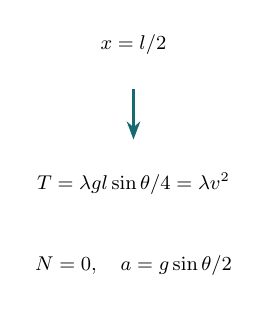
\begin{tikzpicture}[scale=.8,transform shape]
\node at (3,2) {$x=l/2$};\draw[motion] (3,1.3)--(3,.5);\node at (3,-.2) {$T=\lambda gl\sin\theta/4=\lambda v^2$};\node at (3,-1.5) {$N=0,\quad a=g\sin\theta/2$};
\end{tikzpicture}
\figcaption{变图力试2.3V2\quad 领先阶临界接触时，张力恰好全部承担向心动量变化}
\end{minipage}\end{center}

\Needspace{20\baselineskip}
\item 给定初始斜段长$s_0>0$、初速为零，求小圆弧极限的脱离位置。
\textbf{解：}变图力试2.3V3令$s=l-x$，能量给$v^2=(g\sin\theta/l)(s^2-s_0^2)$，加速度仍为$(g\sin\theta/l)s$。法向临界$T=\lambda v^2$变为$s(l-2s)+s_0^2=0$。取下滑区间内的正根$s_{\rm det}=[l+\sqrt{l^2+8s_0^2}]/4$，故$x_{\rm det}=[3l-\sqrt{l^2+8s_0^2}]/4=l/2-s_0^2/l+\cdots$。初始微小斜段趋零时恢复$l/2$。
\begin{center}\begin{minipage}{.98\linewidth}\centering
\begin{tikzpicture}[scale=.8,transform shape]
\draw[axis] (0,0)--(10.7,0) node[right] {$s_0/l$};
\draw[axis] (0,0)--(0,3.2) node[above] {$x_{\rm det}/l$};
\node[above] at (5,3.5) {非零初始斜段使脱离发生在略小的水平绳长};
\draw[traj] plot coordinates {(0.000000000,2.500000000) (0.083333333,2.499944446) (0.166666667,2.499777798) (0.250000000,2.499500100) (0.333333333,2.499111427) (0.416666667,2.498611882) (0.500000000,2.498001597) (0.583333333,2.497280736) (0.666666667,2.496449487) (0.750000000,2.495508071) (0.833333333,2.494456736) (0.916666667,2.493295757) (1.000000000,2.492025437) (1.083333333,2.490646109) (1.166666667,2.489158130) (1.250000000,2.487561883) (1.333333333,2.485857779) (1.416666667,2.484046253) (1.500000000,2.482127767) (1.583333333,2.480102804) (1.666666667,2.477971873) (1.750000000,2.475735506) (1.833333333,2.473394257) (1.916666667,2.470948702) (2.000000000,2.468399438) (2.083333333,2.465747083) (2.166666667,2.462992273) (2.250000000,2.460135666) (2.333333333,2.457177936) (2.416666667,2.454119776) (2.500000000,2.450961894) (2.583333333,2.447705017) (2.666666667,2.444349885) (2.750000000,2.440897254) (2.833333333,2.437347892) (2.916666667,2.433702583) (3.000000000,2.429962122) (3.083333333,2.426127314) (3.166666667,2.422198977) (3.250000000,2.418177940) (3.333333333,2.414065038) (3.416666667,2.409861118) (3.500000000,2.405567034) (3.583333333,2.401183646) (3.666666667,2.396711823) (3.750000000,2.392152439) (3.833333333,2.387506371) (3.916666667,2.382774504) (4.000000000,2.377957727) (4.083333333,2.373056928) (4.166666667,2.368073004) (4.250000000,2.363006849) (4.333333333,2.357859362) (4.416666667,2.352631441) (4.500000000,2.347323986) (4.583333333,2.341937896) (4.666666667,2.336474070) (4.750000000,2.330933405) (4.833333333,2.325316799) (4.916666667,2.319625146) (5.000000000,2.313859338) (5.083333333,2.308020265) (5.166666667,2.302108813) (5.250000000,2.296125865) (5.333333333,2.290072300) (5.416666667,2.283948993) (5.500000000,2.277756814) (5.583333333,2.271496628) (5.666666667,2.265169295) (5.750000000,2.258775671) (5.833333333,2.252316604) (5.916666667,2.245792937) (6.000000000,2.239205507) (6.083333333,2.232555145) (6.166666667,2.225842674) (6.250000000,2.219068911) (6.333333333,2.212234666) (6.416666667,2.205340742) (6.500000000,2.198387935) (6.583333333,2.191377032) (6.666666667,2.184308814) (6.750000000,2.177184054) (6.833333333,2.170003516) (6.916666667,2.162767958) (7.000000000,2.155478128) (7.083333333,2.148134768) (7.166666667,2.140738610) (7.250000000,2.133290379) (7.333333333,2.125790791) (7.416666667,2.118240554) (7.500000000,2.110640369) (7.583333333,2.102990926) (7.666666667,2.095292909) (7.750000000,2.087546993) (7.833333333,2.079753844) (7.916666667,2.071914120) (8.000000000,2.064028470) (8.083333333,2.056097537) (8.166666667,2.048121952) (8.250000000,2.040102342) (8.333333333,2.032039323) (8.416666667,2.023933502) (8.500000000,2.015785480) (8.583333333,2.007595850) (8.666666667,1.999365195) (8.750000000,1.991094090) (8.833333333,1.982783105) (8.916666667,1.974432798) (9.000000000,1.966043723) (9.083333333,1.957616423) (9.166666667,1.949151435) (9.250000000,1.940649288) (9.333333333,1.932110503) (9.416666667,1.923535595) (9.500000000,1.914925070) (9.583333333,1.906279426) (9.666666667,1.897599155) (9.750000000,1.888884743) (9.833333333,1.880136666) (9.916666667,1.871355394) (10.000000000,1.862541391)};
\node[below] at (0,-.12) {$0$};
\node[below] at (5,-.12) {$0.2$};
\node[below] at (10,-.12) {$0.4$};
\end{tikzpicture}
\figcaption{变图力试2.3V3\quad 非零初始斜段使脱离发生在略小的水平绳长}
\end{minipage}\end{center}

\Needspace{20\baselineskip}
\item 有限$r$、圆弧完全被绳占据时，证明支持密度的最小值位于底切点$\phi=\theta$。
\textbf{解：}变图力试2.3V4将主解写成$n/\lambda=(xa-v^2)/r+a\phi+g(2\cos\phi-1)$。其二阶角导数为$-2g\cos\phi<0$，故最小值在两个端点。两端差为$[n(\theta)-n(0)]/\lambda=a\theta-2g(1-\cos\theta)$。由$y\le l-r\theta$，有$a/g\le\sin\theta+(r/l)[1-\cos\theta-\theta\sin\theta]$。在$0<\theta<\pi/2$内，$1-\cos\theta=\sin\theta\tan(\theta/2)<\theta\sin\theta$，故$a<g\sin\theta$，由$\tan(\theta/2)>\theta/2$得$\theta\sin\theta<2(1-\cos\theta)$，故端点差为负。因此先对底切点令$n(\theta)=0$，其余弧段在首次脱离前仍有正支持。
\begin{center}\begin{minipage}{.98\linewidth}\centering
\begin{tikzpicture}[scale=.8,transform shape]
\draw[axis] (0,0)--(8,0) node[right] {$\phi$};\draw[axis] (0,0)--(0,3) node[above] {$n$};\draw[traj] (0,1.8)..controls(3,2)and(5,1.4)..(7,.2);\fill (7,.2) circle(.04) node[right] {$\phi=\theta$最小};\node at (4,-1.5) {$n''(\phi)=-2\lambda g\cos\phi<0$};
\end{tikzpicture}
\figcaption{变图力试2.3V4\quad 支持密度为下凹函数，底切点值又小于顶切点值}
\end{minipage}\end{center}

\Needspace{20\baselineskip}
\item 对初始斜段$s_0>0$且从静止释放的绳，求到脱离的时间，并讨论$s_0\to0$。
\textbf{解：}变图力试2.3V5令$\kappa=\sqrt{g\sin\theta/l}$，运动方程$\dot s^2=\kappa^2(s^2-s_0^2)$的下滑解为$s=s_0\cosh\kappa t$。所以$t_{\rm det}=\kappa^{-1}\operatorname{arcosh}(s_{\rm det}/s_0)$，其中$s_{\rm det}$取变式3的正根。$s_0\to0$时近似$\kappa^{-1}\ln(l/s_0)$，趋于无穷；脱离位置有确定极限，启动等待时间同时受初始扰动控制。
\begin{center}\begin{minipage}{.98\linewidth}\centering
\begin{tikzpicture}[scale=.8,transform shape]
\draw[axis] (0,0)--(10.7,0) node[right] {$s_0/l$};
\draw[axis] (0,0)--(0,3.2) node[above] {$\kappa t_{\rm det}$};
\node[above] at (5,3.5) {初始斜段趋零时，到脱离的等待时间按对数增长};
\draw[traj] plot coordinates {(0.166666667,2.649171182) (0.248611111,2.449239460) (0.330555556,2.306818371) (0.412500000,2.196115015) (0.494444444,2.105549118) (0.576388889,2.028914639) (0.658333333,1.962495659) (0.740277778,1.903890023) (0.822222222,1.851454813) (0.904166667,1.804016672) (0.986111111,1.760708321) (1.068055556,1.720870568) (1.150000000,1.683990636) (1.231944444,1.649661777) (1.313888889,1.617555911) (1.395833333,1.587404562) (1.477777778,1.558985239) (1.559722222,1.532111498) (1.641666667,1.506625549) (1.723611111,1.482392672) (1.805555556,1.459296923) (1.887500000,1.437237800) (1.969444444,1.416127616) (2.051388889,1.395889408) (2.133333333,1.376455253) (2.215277778,1.357764910) (2.297222222,1.339764696) (2.379166667,1.322406571) (2.461111111,1.305647372) (2.543055556,1.289448173) (2.625000000,1.273773749) (2.706944444,1.258592117) (2.788888889,1.243874154) (2.870833333,1.229593260) (2.952777778,1.215725079) (3.034722222,1.202247251) (3.116666667,1.189139197) (3.198611111,1.176381938) (3.280555556,1.163957929) (3.362500000,1.151850922) (3.444444444,1.140045837) (3.526388889,1.128528653) (3.608333333,1.117286312) (3.690277778,1.106306632) (3.772222222,1.095578229) (3.854166667,1.085090449) (3.936111111,1.074833307) (4.018055556,1.064797431) (4.100000000,1.054974012) (4.181944444,1.045354763) (4.263888889,1.035931872) (4.345833333,1.026697973) (4.427777778,1.017646107) (4.509722222,1.008769696) (4.591666667,1.000062512) (4.673611111,0.991518655) (4.755555556,0.983132531) (4.837500000,0.974898827) (4.919444444,0.966812496) (5.001388889,0.958868738) (5.083333333,0.951062982) (5.165277778,0.943390877) (5.247222222,0.935848271) (5.329166667,0.928431204) (5.411111111,0.921135895) (5.493055556,0.913958728) (5.575000000,0.906896249) (5.656944444,0.899945148) (5.738888889,0.893102259) (5.820833333,0.886364547) (5.902777778,0.879729101) (5.984722222,0.873193129) (6.066666667,0.866753949) (6.148611111,0.860408987) (6.230555556,0.854155768) (6.312500000,0.847991910) (6.394444444,0.841915125) (6.476388889,0.835923206) (6.558333333,0.830014030) (6.640277778,0.824185551) (6.722222222,0.818435795) (6.804166667,0.812762858) (6.886111111,0.807164904) (6.968055556,0.801640160) (7.050000000,0.796186911) (7.131944444,0.790803504) (7.213888889,0.785488338) (7.295833333,0.780239864) (7.377777778,0.775056586) (7.459722222,0.769937055) (7.541666667,0.764879867) (7.623611111,0.759883663) (7.705555556,0.754947126) (7.787500000,0.750068980) (7.869444444,0.745247986) (7.951388889,0.740482945) (8.033333333,0.735772691) (8.115277778,0.731116093) (8.197222222,0.726512054) (8.279166667,0.721959508) (8.361111111,0.717457418) (8.443055556,0.713004778) (8.525000000,0.708600610) (8.606944444,0.704243962) (8.688888889,0.699933909) (8.770833333,0.695669550) (8.852777778,0.691450010) (8.934722222,0.687274435) (9.016666667,0.683141995) (9.098611111,0.679051881) (9.180555556,0.675003306) (9.262500000,0.670995502) (9.344444444,0.667027721) (9.426388889,0.663099234) (9.508333333,0.659209329) (9.590277778,0.655357313) (9.672222222,0.651542510) (9.754166667,0.647764259) (9.836111111,0.644021916) (9.918055556,0.640314853) (10.000000000,0.636642456)};
\node[below] at (0,-.12) {$0$};
\node[below] at (5,-.12) {$0.15$};
\node[below] at (10,-.12) {$0.3$};
\end{tikzpicture}
\figcaption{变图力试2.3V5\quad 初始斜段趋零时，到脱离的等待时间按对数增长}
\end{minipage}\end{center}

\Needspace{20\baselineskip}
\item 用整个短弧段的矢量动量通量求支持合力，并求它与竖直方向的夹角。
\textbf{解：}变图力试2.3V6中切向单位矢量由$\boldsymbol t_1=(1,0)$变为$\boldsymbol t_2=(\cos\theta,-\sin\theta)$。领先阶的动量流差为$\lambda v^2(\boldsymbol t_2-\boldsymbol t_1)$，两端张力合力为$T(\boldsymbol t_2-\boldsymbol t_1)$。二者相减得到$\boldsymbol N=(T-\lambda v^2)(1-\cos\theta,\sin\theta)$。故$N_x/N_y=\tan(\theta/2)$，支持合力与竖直方向成$\theta/2$角，其模为$2(T-\lambda v^2)\sin(\theta/2)$。
\begin{center}\begin{minipage}{.98\linewidth}\centering
\begin{tikzpicture}[scale=.8,transform shape]
\draw[motion] (0,0)--(3,0) node[right] {$\boldsymbol t_1$};\draw[motion] (0,0)--(1.5,-2.598076) node[right] {$\boldsymbol t_2$};\draw[force] (0,0)--(1.2,2.07846) node[above] {$\boldsymbol N$};\node at (4,-3.8) {$N_x/N_y=\tan(\theta/2)$};
\end{tikzpicture}
\figcaption{变图力试2.3V6\quad 绳的动量转向与张力合力共同决定向外支持方向}
\end{minipage}\end{center}

\Needspace{20\baselineskip}
\item 固定$0<\theta<\pi/2$，展开有限$r$的脱离位置到$r/l$一阶。
\textbf{解：}变图力试2.3V7令$\epsilon=r/l$、$x/l=1/2+\epsilon\delta+O(\epsilon^2)$，将$y/l=1/2-\epsilon(\delta+\theta)$代入主解的$v^2,a,T(\theta)$。底切点条件给$n(\theta)/(\lambda g)=\delta\sin\theta+\theta\sin\theta+(5\cos\theta-3)/2+O(\epsilon)$。因此$\delta=(3-5\cos\theta)/(2\sin\theta)-\theta$。例如$\theta=\pi/3$时$\delta\simeq-0.758522$，$x_{\rm det}/l\simeq1/2-0.758522(r/l)$。该展开固定转角后令$r/l$变小。
\begin{center}\begin{minipage}{.98\linewidth}\centering
\begin{tikzpicture}[scale=.8,transform shape]
\draw[axis] (0,0)--(10.7,0) node[right] {$r/l$};
\draw[axis] (0,0)--(0,3.2) node[above] {$x_{\rm det}/l$};
\node[above] at (5,3.5) {$\theta=60^\circ$：完整圆弧条件与一阶位置展开};
\draw[traj] plot coordinates {(0.125000000,2.575349403) (0.207291667,2.559122602) (0.289583333,2.542896997) (0.371875000,2.526672588) (0.454166667,2.510449374) (0.536458333,2.494227354) (0.618750000,2.478006528) (0.701041667,2.461786895) (0.783333333,2.445568455) (0.865625000,2.429351206) (0.947916667,2.413135149) (1.030208333,2.396920282) (1.112500000,2.380706604) (1.194791667,2.364494116) (1.277083333,2.348282816) (1.359375000,2.332072703) (1.441666667,2.315863778) (1.523958333,2.299656039) (1.606250000,2.283449486) (1.688541667,2.267244118) (1.770833333,2.251039934) (1.853125000,2.234836933) (1.935416667,2.218635116) (2.017708333,2.202434481) (2.100000000,2.186235028) (2.182291667,2.170036756) (2.264583333,2.153839664) (2.346875000,2.137643752) (2.429166667,2.121449019) (2.511458333,2.105255464) (2.593750000,2.089063087) (2.676041667,2.072871887) (2.758333333,2.056681864) (2.840625000,2.040493016) (2.922916667,2.024305343) (3.005208333,2.008118845) (3.087500000,1.991933520) (3.169791667,1.975749369) (3.252083333,1.959566390) (3.334375000,1.943384583) (3.416666667,1.927203947) (3.498958333,1.911024481) (3.581250000,1.894846185) (3.663541667,1.878669059) (3.745833333,1.862493101) (3.828125000,1.846318311) (3.910416667,1.830144688) (3.992708333,1.813972232) (4.075000000,1.797800942) (4.157291667,1.781630817) (4.239583333,1.765461857) (4.321875000,1.749294061) (4.404166667,1.733127428) (4.486458333,1.716961958) (4.568750000,1.700797650) (4.651041667,1.684634503) (4.733333333,1.668472517) (4.815625000,1.652311692) (4.897916667,1.636152026) (4.980208333,1.619993518) (5.062500000,1.603836170) (5.144791667,1.587679978) (5.227083333,1.571524944) (5.309375000,1.555371066) (5.391666667,1.539218344) (5.473958333,1.523066776) (5.556250000,1.506916364) (5.638541667,1.490767105) (5.720833333,1.474618999) (5.803125000,1.458472046) (5.885416667,1.442326244) (5.967708333,1.426181594) (6.050000000,1.410038095) (6.132291667,1.393895745) (6.214583333,1.377754545) (6.296875000,1.361614494) (6.379166667,1.345475591) (6.461458333,1.329337836) (6.543750000,1.313201227) (6.626041667,1.297065764) (6.708333333,1.280931448) (6.790625000,1.264798276) (6.872916667,1.248666248) (6.955208333,1.232535365) (7.037500000,1.216405624) (7.119791667,1.200277026) (7.202083333,1.184149570) (7.284375000,1.168023255) (7.366666667,1.151898081) (7.448958333,1.135774047) (7.531250000,1.119651152) (7.613541667,1.103529397) (7.695833333,1.087408779) (7.778125000,1.071289299) (7.860416667,1.055170956) (7.942708333,1.039053749) (8.025000000,1.022937678) (8.107291667,1.006822742) (8.189583333,0.990708941) (8.271875000,0.974596274) (8.354166667,0.958484739) (8.436458333,0.942374338) (8.518750000,0.926265069) (8.601041667,0.910156931) (8.683333333,0.894049924) (8.765625000,0.877944047) (8.847916667,0.861839300) (8.930208333,0.845735682) (9.012500000,0.829633192) (9.094791667,0.813531830) (9.177083333,0.797431596) (9.259375000,0.781332488) (9.341666667,0.765234506) (9.423958333,0.749137649) (9.506250000,0.733041917) (9.588541667,0.716947310) (9.670833333,0.700853826) (9.753125000,0.684761465) (9.835416667,0.668670227) (9.917708333,0.652580110) (10.000000000,0.636491115)};
\draw[dashed,thick,color=warm] plot coordinates {(0.125000000,2.575348021) (0.207291667,2.559118802) (0.289583333,2.542889583) (0.371875000,2.526660364) (0.454166667,2.510431145) (0.536458333,2.494201925) (0.618750000,2.477972706) (0.701041667,2.461743487) (0.783333333,2.445514268) (0.865625000,2.429285049) (0.947916667,2.413055829) (1.030208333,2.396826610) (1.112500000,2.380597391) (1.194791667,2.364368172) (1.277083333,2.348138953) (1.359375000,2.331909733) (1.441666667,2.315680514) (1.523958333,2.299451295) (1.606250000,2.283222076) (1.688541667,2.266992857) (1.770833333,2.250763637) (1.853125000,2.234534418) (1.935416667,2.218305199) (2.017708333,2.202075980) (2.100000000,2.185846761) (2.182291667,2.169617541) (2.264583333,2.153388322) (2.346875000,2.137159103) (2.429166667,2.120929884) (2.511458333,2.104700665) (2.593750000,2.088471445) (2.676041667,2.072242226) (2.758333333,2.056013007) (2.840625000,2.039783788) (2.922916667,2.023554568) (3.005208333,2.007325349) (3.087500000,1.991096130) (3.169791667,1.974866911) (3.252083333,1.958637692) (3.334375000,1.942408472) (3.416666667,1.926179253) (3.498958333,1.909950034) (3.581250000,1.893720815) (3.663541667,1.877491596) (3.745833333,1.861262376) (3.828125000,1.845033157) (3.910416667,1.828803938) (3.992708333,1.812574719) (4.075000000,1.796345500) (4.157291667,1.780116280) (4.239583333,1.763887061) (4.321875000,1.747657842) (4.404166667,1.731428623) (4.486458333,1.715199404) (4.568750000,1.698970184) (4.651041667,1.682740965) (4.733333333,1.666511746) (4.815625000,1.650282527) (4.897916667,1.634053308) (4.980208333,1.617824088) (5.062500000,1.601594869) (5.144791667,1.585365650) (5.227083333,1.569136431) (5.309375000,1.552907212) (5.391666667,1.536677992) (5.473958333,1.520448773) (5.556250000,1.504219554) (5.638541667,1.487990335) (5.720833333,1.471761116) (5.803125000,1.455531896) (5.885416667,1.439302677) (5.967708333,1.423073458) (6.050000000,1.406844239) (6.132291667,1.390615019) (6.214583333,1.374385800) (6.296875000,1.358156581) (6.379166667,1.341927362) (6.461458333,1.325698143) (6.543750000,1.309468923) (6.626041667,1.293239704) (6.708333333,1.277010485) (6.790625000,1.260781266) (6.872916667,1.244552047) (6.955208333,1.228322827) (7.037500000,1.212093608) (7.119791667,1.195864389) (7.202083333,1.179635170) (7.284375000,1.163405951) (7.366666667,1.147176731) (7.448958333,1.130947512) (7.531250000,1.114718293) (7.613541667,1.098489074) (7.695833333,1.082259855) (7.778125000,1.066030635) (7.860416667,1.049801416) (7.942708333,1.033572197) (8.025000000,1.017342978) (8.107291667,1.001113759) (8.189583333,0.984884539) (8.271875000,0.968655320) (8.354166667,0.952426101) (8.436458333,0.936196882) (8.518750000,0.919967663) (8.601041667,0.903738443) (8.683333333,0.887509224) (8.765625000,0.871280005) (8.847916667,0.855050786) (8.930208333,0.838821567) (9.012500000,0.822592347) (9.094791667,0.806363128) (9.177083333,0.790133909) (9.259375000,0.773904690) (9.341666667,0.757675470) (9.423958333,0.741446251) (9.506250000,0.725217032) (9.588541667,0.708987813) (9.670833333,0.692758594) (9.753125000,0.676529374) (9.835416667,0.660300155) (9.917708333,0.644070936) (10.000000000,0.627841717)};
\node[below] at (0,-.12) {$0$};
\node[below] at (5,-.12) {$0.02$};
\node[below] at (10,-.12) {$0.04$};
\end{tikzpicture}
\figcaption{变图力试2.3V7\quad $\theta=60^\circ$：完整圆弧条件与一阶位置展开}
\end{minipage}\end{center}

\Needspace{20\baselineskip}
\item 取$\theta=\pi/3,r/l=0.01$，求有限半径脱离位置及底切点的张力、速度关系，量纲用$g=l=\lambda=1$表示。
\textbf{解：}变图力试2.3V8将完整式代入$n(\theta)=0$，得到$x_{\rm det}\simeq0.4924232$，一阶式为0.4924148。此时$v^2\simeq0.2190136$、$a\simeq0.4355054$、$T(\theta)\simeq0.2140136$。两者之差$T-\lambda v^2=-0.005$，除以$r=0.01$后与$\lambda g\cos\theta=0.5$抵消。有限圆弧的临界向心力还包含重力法向分量，正好满足零支持。
\begin{center}\begin{minipage}{.98\linewidth}\centering
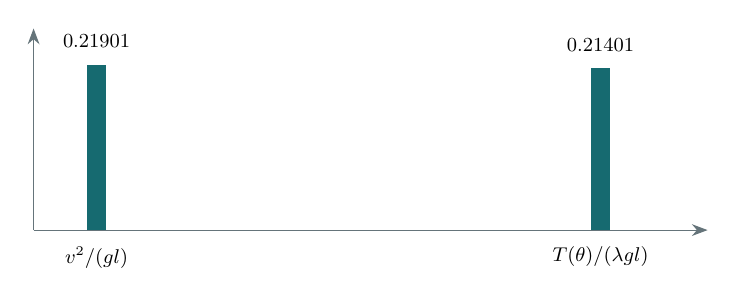
\begin{tikzpicture}[scale=.8,transform shape]
\draw[axis] (0,0)--(10.7,0);
\draw[axis] (0,0)--(0,3.2);
\draw[line width=7pt,color=accent] (1.0,0)--(1.0,2.628162814);
\node[below] at (1.0,-.14) {$v^2/(gl)$};
\node[above] at (1.0,2.768162814) {$ 0.21901 $};
\draw[line width=7pt,color=accent] (9.0,0)--(9.0,2.568162814);
\node[below] at (9.0,-.14) {$T(\theta)/(\lambda gl)$};
\node[above] at (9.0,2.708162814) {$ 0.21401 $};
\end{tikzpicture}
\figcaption{变图力试2.3V8\quad $r/l=0.01,\theta=60^\circ$脱离时的两个法向量}
\end{minipage}\end{center}
\end{enumerate}

\Needspace{13\baselineskip}

\pdfbookmark[2]{第 4 题 两细杆端部弹性碰撞与接触点速度}{q4}

\section*{第 4 题\quad 两细杆端部弹性碰撞与接触点速度}\label{q:4}


光滑水平桌面上，两根均匀细杆$A,B$平行于$x$轴，长度均为$l$，质量分别为$m_A,m_B$。杆$A$静止，位于$x$轴的$(-l+\epsilon,\epsilon)$区域，$0<\epsilon\ll l$。杆$B$位于其下方，横坐标覆盖$(0,l)$，以$v_0\hat y$作无转动平移。

当杆$B$向上到达$x$轴时，其左端与杆$A$右端发生光滑、单点、完全弹性碰撞。取$\epsilon/l\to0$的极限，接触法向沿$y$；忽略杆厚和接触时间内的位移。
\begin{enumerate}
\item 求碰后两杆质心的带符号速度$v_A,v_B$及角速度$\omega_A,\omega_B$，其中向$+y$、逆时针分别为正。
\item 验证
\[
v_0=\left(v_A+\frac l2\omega_A\right)
-\left(v_B-\frac l2\omega_B\right),
\]
并说明它在本题中的物理依据和适用条件。
\end{enumerate}


\begin{center}\begin{minipage}{.98\linewidth}\centering
\begin{tikzpicture}[scale=.9,transform shape]
\draw[axis] (0.00000,0.00000)--(5.25000,0.00000);\draw[axis] (0.00000,-2.20000)--(0.00000,2.25000);\node[below right] at (5.25000,0.00000) {$x$};\node[above right] at (0.00000,2.25000) {$y$};\draw[very thick,color=accent] (-4.00000,0.00000)--(0.00000,0.00000);\draw[very thick,color=accent] (0.00000,-1.50000)--(4.00000,-1.50000);\node[below] at (-2.00000,-0.10000) {杆 $A,m_A$};\node[below] at (2.00000,-1.60000) {杆 $B,m_B$};\draw[motion] (2.00000,-1.40000)--(2.00000,-0.30000);\node[right] at (2.10000,-0.70000) {$v_0$};\fill (0.00000,0.00000) circle(.035);\node[below left] at (0.00000,0.00000) {$O$};
\end{tikzpicture}
\figcaption{图力试2.4\quad B杆向+y平移，端部将与静止A杆接触，取小重叠极限。}
\end{minipage}\end{center}

\Needspace{8\baselineskip}

\pdfbookmark[3]{题型定位}{q4-h0}

\subsection*{题型定位}

两根杆在端部交换一个法向冲量，同时获得质心速度和绕质心的角速度。题目的四个运动量由逐杆冲量方程联系，再由总动能确定非零碰撞冲量。第二问将同一结果换成接触点语言，比较端部在碰前的接近速率与碰后的分离速率。

\Needspace{8\baselineskip}

\pdfbookmark[3]{知识点}{q4-h1}

\subsection*{知识点}

均匀杆的质心惯量为$ml^2/12$，端部力臂为$l/2$；平动冲量与角冲量分别确定$v$和$\omega$。刚体接触点速度由质心平移和绕质心转动叠加。总动能同时包含两杆的平动能与转动能，接触点的有效逆质量由$1/m$和$d^2/I$相加而成。总线动量、关于固定点的轨道角动量与自转角动量，则提供另一种组织同组方程的方式。

\Needspace{8\baselineskip}

\pdfbookmark[3]{物理图像}{q4-h2}

\subsection*{物理图像}

解图力试2.4A中，杆$A$在质心右侧受向上冲量，杆$B$在质心左侧受向下冲量，两角冲量都指向纸外。图B用等质量情形展示碰后端点：$A$右端以$v_0$上行，$B$左端瞬时静止，而两个质心均上行。图C把整个接触过程中累计冲量与总动能联系起来，动能先降后升，完全弹性终态取第二个与初态等能的交点。

\Needspace{8\baselineskip}

\pdfbookmark[3]{解题入口}{q4-h3}

\subsection*{解题入口}

在图A的同一个接触位置画$+J\hat y$与$-J\hat y$，逐杆写出$v_A,v_B,\omega_A,\omega_B$。由这些表达式构造总动能，平动与转动的四个未知量便统一写成同一个冲量的函数。求得$J$后，在图B标出的左右端点分别使用$v_A+l\omega_A/2$和$v_B-l\omega_B/2$，两式的转动项符号由端点相对各自质心的位置确定。

\Needspace{8\baselineskip}

\pdfbookmark[3]{标准解法}{q4-h4}

\subsection*{标准解法}


图力试2.4中的接触冲量作用在两杆相对的端部。设杆$A$受到$+J\hat y$，杆$B$受到$-J\hat y$，其中$J>0$。

\begin{center}\begin{minipage}{.98\linewidth}\centering
\begin{tikzpicture}[scale=.82,transform shape]
\draw[very thick,color=accent] (-4.00000,0.00000)--(0.00000,0.00000);\draw[very thick,color=ink] (0.00000,0.00000)--(4.00000,0.00000);\fill (-2.00000,0.00000) circle(.035);\node[below] at (-2.00000,0.00000) {$C_A$};\fill (2.00000,0.00000) circle(.035);\node[below] at (2.00000,0.00000) {$C_B$};\draw[force] (-0.12000,0.00000)--(-0.12000,1.70000);\node[above left] at (-0.20000,1.70000) {$+J$};\draw[force] (0.12000,0.00000)--(0.12000,-1.70000);\node[below right] at (0.20000,-1.70000) {$-J$};\draw[motion] plot coordinates {(-1.15425,0.08486) (-1.15840,0.11924) (-1.16396,0.15341) (-1.17090,0.18734) (-1.17922,0.22095) (-1.18890,0.25420) (-1.19993,0.28702) (-1.21228,0.31937) (-1.22594,0.35119) (-1.24089,0.38243) (-1.25709,0.41303) (-1.27453,0.44294) (-1.29318,0.47212) (-1.31299,0.50052) (-1.33395,0.52808) (-1.35601,0.55477) (-1.37914,0.58054) (-1.40330,0.60535) (-1.42845,0.62915) (-1.45455,0.65191) (-1.48155,0.67358) (-1.50942,0.69414) (-1.53810,0.71354) (-1.56754,0.73177) (-1.59771,0.74877) (-1.62854,0.76454) (-1.65998,0.77903) (-1.69200,0.79223) (-1.72452,0.80412) (-1.75750,0.81467) (-1.79088,0.82387) (-1.82461,0.83171) (-1.85863,0.83816) (-1.89289,0.84322) (-1.92732,0.84689) (-1.96187,0.84914) (-1.99649,0.84999) (-2.03111,0.84943) (-2.06568,0.84746) (-2.10015,0.84408) (-2.13444,0.83930) (-2.16851,0.83313) (-2.20231,0.82557) (-2.23576,0.81665) (-2.26883,0.80637) (-2.30145,0.79475) (-2.33357,0.78181) (-2.36514,0.76758) (-2.39610,0.75207) (-2.42640,0.73531) (-2.45599,0.71734) (-2.48483,0.69817) (-2.51287,0.67784) (-2.54005,0.65639) (-2.56633,0.63385)};\node[above] at (-2.00000,1.30000) {$\omega_A>0$};\draw[motion] plot coordinates {(2.84575,0.08486) (2.84160,0.11924) (2.83604,0.15341) (2.82910,0.18734) (2.82078,0.22095) (2.81110,0.25420) (2.80007,0.28702) (2.78772,0.31937) (2.77406,0.35119) (2.75911,0.38243) (2.74291,0.41303) (2.72547,0.44294) (2.70682,0.47212) (2.68701,0.50052) (2.66605,0.52808) (2.64399,0.55477) (2.62086,0.58054) (2.59670,0.60535) (2.57155,0.62915) (2.54545,0.65191) (2.51845,0.67358) (2.49058,0.69414) (2.46190,0.71354) (2.43246,0.73177) (2.40229,0.74877) (2.37146,0.76454) (2.34002,0.77903) (2.30800,0.79223) (2.27548,0.80412) (2.24250,0.81467) (2.20912,0.82387) (2.17539,0.83171) (2.14137,0.83816) (2.10711,0.84322) (2.07268,0.84689) (2.03813,0.84914) (2.00351,0.84999) (1.96889,0.84943) (1.93432,0.84746) (1.89985,0.84408) (1.86556,0.83930) (1.83149,0.83313) (1.79769,0.82557) (1.76424,0.81665) (1.73117,0.80637) (1.69855,0.79475) (1.66643,0.78181) (1.63486,0.76758) (1.60390,0.75207) (1.57360,0.73531) (1.54401,0.71734) (1.51517,0.69817) (1.48713,0.67784) (1.45995,0.65639) (1.43367,0.63385)};\node[above] at (2.00000,1.30000) {$\omega_B>0$};\draw[<->,thin,color=muted] (-2.00000,-2.50000)--(0.00000,-2.50000);\node[below] at (-1.00000,-2.50000) {$l/2$};\draw[<->,thin,color=muted] (0.00000,-3.50000)--(2.00000,-3.50000);\node[below] at (1.00000,-3.50000) {$l/2$};\node[above] at (0.00000,2.80000) {冲量相反，绕各自质心的力矩同向};
\end{tikzpicture}
\figcaption{解图力试2.4A\quad 两端接触冲量关于杆质心产生同向角冲量。}
\end{minipage}\end{center}
解图力试2.4A标明关于各自质心的力臂：杆$A$在右端受向上冲量，杆$B$在左端受向下冲量，两者都产生逆时针角冲量。由平动与转动冲量方程，
\[
v_A=\frac{J}{m_A},\qquad
v_B=v_0-\frac{J}{m_B},
\]
\[
I_A\omega_A=\frac{Jl}{2},\quad
I_B\omega_B=\frac{Jl}{2},\quad
I_A=\frac{m_Al^2}{12},\ I_B=\frac{m_Bl^2}{12}.
\]
因此
\[
\omega_A=\frac{6J}{m_Al},\qquad
\omega_B=\frac{6J}{m_Bl}.
\]
用同一个接触冲量表示四个速度后，总动能就成为冲量的一元二次函数；逐杆角冲量同时给出两杆角速度的联系。

（1）完全弹性刚体模型要求碰前、碰后的总平动加转动动能相同。把上述速度代入，动能改变量为
\[
\Delta K=-Jv_0+
\frac{J^2}{2}
\left(\frac1{m_A}+\frac1{m_B}
+\frac{(l/2)^2}{I_A}+\frac{(l/2)^2}{I_B}\right).
\]
其中两项$1/m$来自质心平动，两项$(l/2)^2/I$来自绕质心转动。每项转动响应等于$3/m$，所以转动能与平动能共同决定接触的惯性。记接触点的有效逆质量
\[
\mathcal K=
\frac1{m_A}+\frac1{m_B}
+\frac{(l/2)^2}{I_A}+\frac{(l/2)^2}{I_B}
=4\left(\frac1{m_A}+\frac1{m_B}\right).
\]
\begin{center}\begin{minipage}{.98\linewidth}\centering
\begin{tikzpicture}[scale=.8,transform shape]
\draw[axis] (0,0)--(8.5,0) node[right] {$J/J_{\rm el}$};
\draw[axis] (0,0)--(0,3.2) node[above] {$\mathcal K\Delta K/v_0^2$};
\node[above] at (5,3.5) {累计冲量增大：总动能先降后回到初值};
\draw[traj] plot coordinates {(0.000000000,2.000000000) (0.080000000,1.920800000) (0.160000000,1.843200000) (0.240000000,1.767200000) (0.320000000,1.692800000) (0.400000000,1.620000000) (0.480000000,1.548800000) (0.560000000,1.479200000) (0.640000000,1.411200000) (0.720000000,1.344800000) (0.800000000,1.280000000) (0.880000000,1.216800000) (0.960000000,1.155200000) (1.040000000,1.095200000) (1.120000000,1.036800000) (1.200000000,0.980000000) (1.280000000,0.924800000) (1.360000000,0.871200000) (1.440000000,0.819200000) (1.520000000,0.768800000) (1.600000000,0.720000000) (1.680000000,0.672800000) (1.760000000,0.627200000) (1.840000000,0.583200000) (1.920000000,0.540800000) (2.000000000,0.500000000) (2.080000000,0.460800000) (2.160000000,0.423200000) (2.240000000,0.387200000) (2.320000000,0.352800000) (2.400000000,0.320000000) (2.480000000,0.288800000) (2.560000000,0.259200000) (2.640000000,0.231200000) (2.720000000,0.204800000) (2.800000000,0.180000000) (2.880000000,0.156800000) (2.960000000,0.135200000) (3.040000000,0.115200000) (3.120000000,0.096800000) (3.200000000,0.080000000) (3.280000000,0.064800000) (3.360000000,0.051200000) (3.440000000,0.039200000) (3.520000000,0.028800000) (3.600000000,0.020000000) (3.680000000,0.012800000) (3.760000000,0.007200000) (3.840000000,0.003200000) (3.920000000,0.000800000) (4.000000000,0.000000000) (4.080000000,0.000800000) (4.160000000,0.003200000) (4.240000000,0.007200000) (4.320000000,0.012800000) (4.400000000,0.020000000) (4.480000000,0.028800000) (4.560000000,0.039200000) (4.640000000,0.051200000) (4.720000000,0.064800000) (4.800000000,0.080000000) (4.880000000,0.096800000) (4.960000000,0.115200000) (5.040000000,0.135200000) (5.120000000,0.156800000) (5.200000000,0.180000000) (5.280000000,0.204800000) (5.360000000,0.231200000) (5.440000000,0.259200000) (5.520000000,0.288800000) (5.600000000,0.320000000) (5.680000000,0.352800000) (5.760000000,0.387200000) (5.840000000,0.423200000) (5.920000000,0.460800000) (6.000000000,0.500000000) (6.080000000,0.540800000) (6.160000000,0.583200000) (6.240000000,0.627200000) (6.320000000,0.672800000) (6.400000000,0.720000000) (6.480000000,0.768800000) (6.560000000,0.819200000) (6.640000000,0.871200000) (6.720000000,0.924800000) (6.800000000,0.980000000) (6.880000000,1.036800000) (6.960000000,1.095200000) (7.040000000,1.155200000) (7.120000000,1.216800000) (7.200000000,1.280000000) (7.280000000,1.344800000) (7.360000000,1.411200000) (7.440000000,1.479200000) (7.520000000,1.548800000) (7.600000000,1.620000000) (7.680000000,1.692800000) (7.760000000,1.767200000) (7.840000000,1.843200000) (7.920000000,1.920800000) (8.000000000,2.000000000)};
\node[below] at (0,-.12) {$0$};
\node[below] at (4,-.12) {$1/2$};
\node[below] at (8,-.12) {$1$};
\draw[guide] (0,2)--(8.2,2) node[right] {$\Delta K=0$};\node[left] at (0,0) {$-1/2$};\node[left] at (0,2) {$0$};\end{tikzpicture}
\figcaption{解图力试2.4C\quad 累计冲量增大：总动能先降后回到初值}
\end{minipage}\end{center}
图C的横坐标用最终弹性冲量$J_{\rm el}$归一化，纵坐标表示$\mathcal K\Delta K/v_0^2$，水平虚线对应总动能回到碰前值。累计冲量从零增大时，刚体动能转入接触形变能，在$J=v_0/\mathcal K$处最低，此时两端法向速度相同；随后形变恢复，累计冲量继续增加，动能回到碰前值。由$\Delta K=0$，除去没有发生碰撞的$J=0$根，得
\[
\boxed{J=\frac{2v_0}{\mathcal K}
=\frac{m_Am_B}{2(m_A+m_B)}v_0}.
\]
于是
\[
\boxed{v_A=\frac{m_B}{2(m_A+m_B)}v_0,\qquad
v_B=\frac{m_A+2m_B}{2(m_A+m_B)}v_0},
\]
\[
\boxed{\omega_A=\frac{3m_B}{l(m_A+m_B)}v_0,\qquad
\omega_B=\frac{3m_A}{l(m_A+m_B)}v_0}.
\]
两杆质心都向上运动，两角速度也都为正。相反的接触冲量作用在相反侧的端部，因而绕各自质心都产生逆时针转动。

\begin{center}\begin{minipage}{.98\linewidth}\centering
\begin{tikzpicture}[scale=.83,transform shape]
\draw[very thick,color=accent] (-4.00000,0.00000)--(0.00000,0.00000);\draw[very thick,color=ink] (0.00000,-3.00000)--(4.00000,-3.00000);\draw[motion] (-2.00000,0.00000)--(-2.00000,0.60000);\node[above left] at (-2.00000,0.60000) {$v_A=v_0/4$};\draw[force] (0.00000,0.00000)--(0.00000,2.40000);\node[above right] at (0.00000,2.40000) {$u_A=v_0$};\draw[motion] (2.00000,-3.00000)--(2.00000,-1.20000);\node[above right] at (2.00000,-1.20000) {$v_B=3v_0/4$};\fill (0.00000,-3.00000) circle(.035);\node[below left] at (0.00000,-3.00000) {$u_B=0$};\node[above] at (0.00000,3.50000) {等质量示例：$m_A=m_B$};\node[below] at (0.00000,-4.40000) {恢复关系比较端点，不只比较质心};
\end{tikzpicture}
\figcaption{解图力试2.4B\quad 等质量时的质心与接触点速度，uB恰为零。}
\end{minipage}\end{center}
（2）解图力试2.4B把接触点速度与质心速度分开，箭头取等质量的情形举例。一般情况下，杆$A$右端和杆$B$左端的碰后法向速度分别为
\[
u_A=v_A+\frac l2\omega_A=\frac{4J}{m_A},
\qquad
u_B=v_B-\frac l2\omega_B=v_0-\frac{4J}{m_B}.
\]
所以
\[
u_A-u_B=\mathcal KJ-v_0=v_0,
\]
即
\[
\boxed{v_0=
\left(v_A+\frac l2\omega_A\right)
-\left(v_B-\frac l2\omega_B\right)}.
\]
碰前接近速率为$v_0$，碰后分离速率也为$v_0$，这是恢复系数为1的接触关系。这个关系由完整刚体的能量与冲量方程直接推出，也适用于这里的两杆端部碰撞。

本题取光滑单点法向接触，碰前、碰后均以完整刚体描述，完全弹性过程回收接触时暂存的形变能。端部质元受到杆内力，计算时把整杆的平动与转动一并计入，端点速度按$v\pm(l/2)\omega$合成。摩擦接触需增加切向冲量，多点接触需联立各接触约束，若振动仍储存能量，则把它计入碰后的能量分配。

总动量给$m_Av_A+m_Bv_B=m_Bv_0$。关于接触点的总角动量，则由两杆质心的轨道角动量与各自绕质心的自转角动量共同组成。
把这一总角动量展开，以接触点$O$为固定点，有
\[
\frac l2m_Bv_0=\frac l2m_Bv_B-\frac l2m_Av_A+I_A\omega_A+I_B\omega_B.
\]
式中$A$质心位于$O$左侧，故其向上平移的轨道项为负；$B$位于右侧，其轨道项为正。把冲量方程代入，右侧相对碰前的变化为$-Jl/2-Jl/2+Jl/2+Jl/2=0$，轨道角动量的减少恰好转为两杆的自转角动量。进一步由角冲量得$m_A\omega_A=m_B\omega_B$，与总动量、总角动量联立便得到$\omega_A=6v_A/l$、$\omega_B=6m_Av_A/(m_Bl)$和$v_B=v_0-m_Av_A/m_B$，与以$J$为变量的写法相同。

能量式的两根分别是$J=0$与$2v_0/\mathcal K$。碰前两接触端正在接近，光滑单侧接触会产生正法向冲量，所以弹性终态取第二根。此时$u_A-u_B=v_0>0$，两杆端部沿法向分开；质心速度差与端点分离速率分别对应不同的图中对象。接触时间趋零保证计算角冲量时可固定力臂，$\epsilon/l\to0$则把实际短重叠接触的位置化为所画的端部极限。



\Needspace{8\baselineskip}

\pdfbookmark[3]{关键洞察}{q4-h5}

\subsection*{关键洞察}

接触点的速度变化含有质心响应$J/m$和转动响应$Jd^2/I$。细杆端部的转动响应是平动响应的3倍，故每杆在接触点贡献$4/m$的有效逆质量。两杆相互作用的功由完整刚体的动能计算；单独抽出端部质元会引入杆内部的力和功，完整的冲量—动能方程则直接给出本题的端点恢复关系。

\Needspace{8\baselineskip}

\pdfbookmark[3]{易错点}{q4-h6}

\subsection*{易错点}

判断转动方向时同时使用力臂和冲量：$A$为$(+\hat x)\times(+\hat y)$，$B$为$(-\hat x)\times(-\hat y)$，两者都是$+\hat z$。动能方程中保留两项转动能，端点相对速度用$u_A-u_B$。能量方程的$J=0$根描述保持碰前速度的状态，实际接触取正的第二根。恢复条件在这里依赖光滑、单点法向接触和完整刚体完全弹性的条件；摩擦、多点接触或振动能储存应分别计入相应的冲量与能量方程。

\Needspace{8\baselineskip}

\pdfbookmark[3]{课堂讲解建议}{q4-h7}

\subsection*{课堂讲解建议}

先请学生在图A上用叉乘判断两个角冲量，再列代数方程。由同一个$J$算出平动、转动响应后，追问：“细杆端点为何比质心对同一冲量响应更大？”让学生算出$3/m$与$1/m$，再合成$\mathcal K$。在图C中指出最大压缩时的能量最低点，完全弹性过程继续回到初始动能。

第二问让学生先对图B的等质量例子报出四个速度，再写一般的端点速度差。随后把$\Delta K=-Jv_0+\mathcal KJ^2/2$与$u_A-u_B=\mathcal KJ-v_0$并列，说明非零等能根为何给分离速率$v_0$。最后由关于$O$的角动量式辨认轨道项与自转项，让学生看见总守恒法与逐杆冲量法怎样描述同一次碰撞。

\Needspace{8\baselineskip}

\pdfbookmark[3]{变式训练}{q4-h8}

\subsection*{变式训练}

\begin{enumerate}
\Needspace{20\baselineskip}
\item 令$m_A=m_B=m$，求两质心、两角速度和两个接触点速度。
\textbf{解：}变图力试2.4V1在两个质心处标出平动箭头，在端部标出合成箭头。此时$\mathcal K=8/m$，所以$J=mv_0/4$。平动给$v_A=v_0/4,v_B=3v_0/4$，角冲量给$\omega_A=\omega_B=3v_0/(2l)$。$A$右端的转动速度向上，$u_A=v_0/4+3v_0/4=v_0$；$B$左端的转动速度向下，$u_B=3v_0/4-3v_0/4=0$。因此两个接触点以$v_0$分离，两个质心仍均向上。
\begin{center}\begin{minipage}{.98\linewidth}\centering
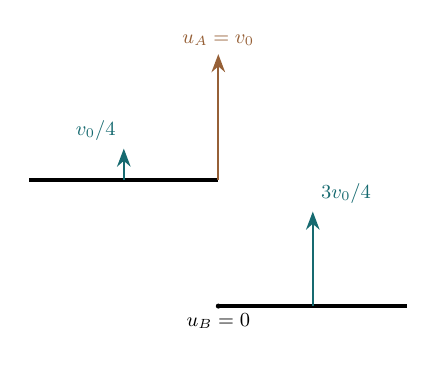
\begin{tikzpicture}[scale=.8,transform shape]
\draw[very thick] (-3,0)--(0,0);\draw[very thick] (0,-2)--(3,-2);\draw[motion] (-1.5,0)--(-1.5,.5) node[above left] {$v_0/4$};\draw[force] (0,0)--(0,2) node[above] {$u_A=v_0$};\draw[motion] (1.5,-2)--(1.5,-.5) node[above right] {$3v_0/4$};\fill (0,-2) circle(.04) node[below] {$u_B=0$};
\end{tikzpicture}
\figcaption{变图力试2.4V1\quad 等质量杆的质心与端部速度}
\end{minipage}\end{center}

\Needspace{20\baselineskip}
\item 将法向恢复系数改为$e\in[0,1]$，求冲量和损失的动能。
\textbf{解：}变图力试2.4V2沿同一法向画出碰前接近与碰后分离。冲量后的端点差为$\mathcal KJ-v_0$，恢复条件令其等于$ev_0$，故$J=(1+e)v_0/\mathcal K$。代入总动能改变量，$\Delta K=-(1-e^2)v_0^2/(2\mathcal K)$，即损失$Q=(1-e^2)v_0^2/(2\mathcal K)$。当$e=0$时两个接触点具有共同法向速度，两杆仍按各自的$v,\omega$运动；当$e=1$时$Q=0$，恢复本题的完全弹性结果。
\begin{center}\begin{minipage}{.98\linewidth}\centering
\begin{tikzpicture}[scale=.8,transform shape]
\draw[axis] (0,0)--(10.7,0) node[right] {$e$};
\draw[axis] (0,0)--(0,3.2) node[above] {$2\mathcal KQ/v_0^2$};
\node[above] at (5,3.5) {法向恢复系数与耗散能};
\draw[traj] plot coordinates {(0.000000000,2.500000000) (0.100000000,2.499750000) (0.200000000,2.499000000) (0.300000000,2.497750000) (0.400000000,2.496000000) (0.500000000,2.493750000) (0.600000000,2.491000000) (0.700000000,2.487750000) (0.800000000,2.484000000) (0.900000000,2.479750000) (1.000000000,2.475000000) (1.100000000,2.469750000) (1.200000000,2.464000000) (1.300000000,2.457750000) (1.400000000,2.451000000) (1.500000000,2.443750000) (1.600000000,2.436000000) (1.700000000,2.427750000) (1.800000000,2.419000000) (1.900000000,2.409750000) (2.000000000,2.400000000) (2.100000000,2.389750000) (2.200000000,2.379000000) (2.300000000,2.367750000) (2.400000000,2.356000000) (2.500000000,2.343750000) (2.600000000,2.331000000) (2.700000000,2.317750000) (2.800000000,2.304000000) (2.900000000,2.289750000) (3.000000000,2.275000000) (3.100000000,2.259750000) (3.200000000,2.244000000) (3.300000000,2.227750000) (3.400000000,2.211000000) (3.500000000,2.193750000) (3.600000000,2.176000000) (3.700000000,2.157750000) (3.800000000,2.139000000) (3.900000000,2.119750000) (4.000000000,2.100000000) (4.100000000,2.079750000) (4.200000000,2.059000000) (4.300000000,2.037750000) (4.400000000,2.016000000) (4.500000000,1.993750000) (4.600000000,1.971000000) (4.700000000,1.947750000) (4.800000000,1.924000000) (4.900000000,1.899750000) (5.000000000,1.875000000) (5.100000000,1.849750000) (5.200000000,1.824000000) (5.300000000,1.797750000) (5.400000000,1.771000000) (5.500000000,1.743750000) (5.600000000,1.716000000) (5.700000000,1.687750000) (5.800000000,1.659000000) (5.900000000,1.629750000) (6.000000000,1.600000000) (6.100000000,1.569750000) (6.200000000,1.539000000) (6.300000000,1.507750000) (6.400000000,1.476000000) (6.500000000,1.443750000) (6.600000000,1.411000000) (6.700000000,1.377750000) (6.800000000,1.344000000) (6.900000000,1.309750000) (7.000000000,1.275000000) (7.100000000,1.239750000) (7.200000000,1.204000000) (7.300000000,1.167750000) (7.400000000,1.131000000) (7.500000000,1.093750000) (7.600000000,1.056000000) (7.700000000,1.017750000) (7.800000000,0.979000000) (7.900000000,0.939750000) (8.000000000,0.900000000) (8.100000000,0.859750000) (8.200000000,0.819000000) (8.300000000,0.777750000) (8.400000000,0.736000000) (8.500000000,0.693750000) (8.600000000,0.651000000) (8.700000000,0.607750000) (8.800000000,0.564000000) (8.900000000,0.519750000) (9.000000000,0.475000000) (9.100000000,0.429750000) (9.200000000,0.384000000) (9.300000000,0.337750000) (9.400000000,0.291000000) (9.500000000,0.243750000) (9.600000000,0.196000000) (9.700000000,0.147750000) (9.800000000,0.099000000) (9.900000000,0.049750000) (10.000000000,0.000000000)};
\node[below] at (0,-.12) {$0$};
\node[below] at (5,-.12) {$1/2$};
\node[below] at (10,-.12) {$1$};
\end{tikzpicture}
\figcaption{变图力试2.4V2\quad 法向恢复系数与耗散能}
\end{minipage}\end{center}

\Needspace{20\baselineskip}
\item 保留光滑单点接触，令两接触力臂为$d_A,d_B$，质心惯量为任意$I_A,I_B$，求一般冲量。
\textbf{解：}变图力试2.4V3将力臂分别标在两刚体上，接触法向与力臂垂直。平动速度变化仍为$J/m_A,-J/m_B$，转动响应在接触点分别贡献$Jd_A^2/I_A,Jd_B^2/I_B$。故$\mathcal K=1/m_A+1/m_B+d_A^2/I_A+d_B^2/I_B$，而$u_A-u_B=-v_0+\mathcal KJ$。给定恢复系数$e$后，$J=(1+e)v_0/\mathcal K$，再以$\omega_A=Jd_A/I_A,\omega_B=Jd_B/I_B$恢复角速度。有效接触质量为$1/\mathcal K$，同时反映平动和转动。
\begin{center}\begin{minipage}{.98\linewidth}\centering
\begin{tikzpicture}[scale=.8,transform shape]
\draw[very thick] (-3,0)--(0,0);\draw[very thick] (0,-1)--(4,-1);\fill (-2,0) circle(.04) node[above] {$C_A$};\fill (2.8,-1) circle(.04) node[below] {$C_B$};\draw[force] (0,0)--(0,1.5) node[above] {$J$};\draw[force] (0,-1)--(0,-2.5) node[below] {$-J$};\draw[<->] (-2,-.5)--(0,-.5) node[midway,below] {$d_A$};\draw[<->] (0,-3.5)--(2.8,-3.5) node[midway,below] {$d_B$};
\end{tikzpicture}
\figcaption{变图力试2.4V3\quad 任意惯量刚体在接触点的平动与转动响应}
\end{minipage}\end{center}

\Needspace{20\baselineskip}
\item 令$m_A\to\infty$且长度不变，求杆$B$碰后质心和接触端速度。
\textbf{解：}变图力试2.4V4把重杆作为静止接触面。极限下$v_A,\omega_A\to0$，$J\to m_Bv_0/2$，所以$v_B=v_0-J/m_B=v_0/2$、$\omega_B=6J/(m_Bl)=3v_0/l$。杆$B$左端的转动分量为$-l\omega_B/2=-3v_0/2$，与质心的$v_0/2$相加得到$u_B=-v_0$。接触端向下弹回，质心仍向上；向上的质心平动能为初始能量的$1/4$，其余$3/4$变成绕质心的转动能。
\begin{center}\begin{minipage}{.98\linewidth}\centering
\begin{tikzpicture}[scale=.8,transform shape]
\draw[very thick] (-2,0)--(0,0);\node[above] at (-1,0) {$A$静止};\draw[very thick] (0,-1)--(4,-1);\draw[motion] (2,-1)--(2,0) node[above] {$v_B=v_0/2$};\draw[force] (0,-1)--(0,-3) node[below] {$u_B=-v_0$};\node[right] at (4,-1) {$\omega_B=3v_0/l$};
\end{tikzpicture}
\figcaption{变图力试2.4V4\quad 重杆极限：接触端弹回而质心继续向上}
\end{minipage}\end{center}

\Needspace{20\baselineskip}
\item 求完全弹性碰撞后，两杆转动动能之和占初始动能的比例，并讨论质量比。
\textbf{解：}变图力试2.4V5令$r=m_A/m_B$。由$I\omega^2/2=3J^2/(2m)$，两杆转动能总和为$K_{\rm rot}=3J^2(1/m_A+1/m_B)/2=3m_Am_Bv_0^2/[8(m_A+m_B)]$。除以初始$K_0=m_Bv_0^2/2$得到$K_{\rm rot}/K_0=3r/[4(1+r)]$。其导数为$3/[4(1+r)^2]>0$，等质量时为$3/8$，重杆极限趋向$3/4$。图中曲线正按这个比例绘制，增加的是碰后转动能占比。
\begin{center}\begin{minipage}{.98\linewidth}\centering
\begin{tikzpicture}[scale=.8,transform shape]
\draw[axis] (0,0)--(10.7,0) node[right] {$r=m_A/m_B$};
\draw[axis] (0,0)--(0,3.2) node[above] {$K_{\rm rot}/K_0$};
\node[above] at (5,3.5) {转动能占比随静止杆质量增大};
\draw[traj] plot coordinates {(0.020000000,0.029702970) (0.086533333,0.124416896) (0.153066667,0.213277186) (0.219600000,0.296810236) (0.286133333,0.375481162) (0.352666667,0.449702465) (0.419200000,0.519841270) (0.485733333,0.586225393) (0.552266667,0.649148469) (0.618800000,0.708874294) (0.685333333,0.765640516) (0.751866667,0.819661805) (0.818400000,0.871132557) (0.884933333,0.920229237) (0.951466667,0.967112396) (1.018000000,1.011928429) (1.084533333,1.054811101) (1.151066667,1.095882876) (1.217600000,1.135256091) (1.284133333,1.173033982) (1.350666667,1.209311580) (1.417200000,1.244176519) (1.483733333,1.277709737) (1.550266667,1.309986104) (1.616800000,1.341074983) (1.683333333,1.371040724) (1.749866667,1.399943109) (1.816400000,1.427837753) (1.882933333,1.454776458) (1.949466667,1.480807535) (2.016000000,1.505976096) (2.082533333,1.530324308) (2.149066667,1.553891638) (2.215600000,1.576715058) (2.282133333,1.598829244) (2.348666667,1.620266748) (2.415200000,1.641058163) (2.481733333,1.661232261) (2.548266667,1.680816135) (2.614800000,1.699835312) (2.681333333,1.718313871) (2.747866667,1.736274537) (2.814400000,1.753738784) (2.880933333,1.770726910) (2.947466667,1.787258125) (3.014000000,1.803350618) (3.080533333,1.819021625) (3.147066667,1.834287491) (3.213600000,1.849163726) (3.280133333,1.863665059) (3.346666667,1.877805486) (3.413200000,1.891598315) (3.479733333,1.905056207) (3.546266667,1.918191216) (3.612800000,1.931014823) (3.679333333,1.943537974) (3.745866667,1.955771105) (3.812400000,1.967724176) (3.878933333,1.979406695) (3.945466667,1.990827746) (4.012000000,2.001996008) (4.078533333,2.012919783) (4.145066667,2.023607013) (4.211600000,2.034065297) (4.278133333,2.044301916) (4.344666667,2.054323842) (4.411200000,2.064137759) (4.477733333,2.073750077) (4.544266667,2.083166945) (4.610800000,2.092394264) (4.677333333,2.101437700) (4.743866667,2.110302695) (4.810400000,2.118994479) (4.876933333,2.127518080) (4.943466667,2.135878332) (5.010000000,2.144079886) (5.076533333,2.152127219) (5.143066667,2.160024639) (5.209600000,2.167776298) (5.276133333,2.175386194) (5.342666667,2.182858180) (5.409200000,2.190195973) (5.475733333,2.197403153) (5.542266667,2.204483179) (5.608800000,2.211439386) (5.675333333,2.218274993) (5.741866667,2.224993111) (5.808400000,2.231596742) (5.874933333,2.238088788) (5.941466667,2.244472054) (6.008000000,2.250749251) (6.074533333,2.256923001) (6.141066667,2.262995840) (6.207600000,2.268970223) (6.274133333,2.274848524) (6.340666667,2.280633043) (6.407200000,2.286326006) (6.473733333,2.291929571) (6.540266667,2.297445825) (6.606800000,2.302876795) (6.673333333,2.308224443) (6.739866667,2.313490671) (6.806400000,2.318677326) (6.872933333,2.323786196) (6.939466667,2.328819020) (7.006000000,2.333777482) (7.072533333,2.338663218) (7.139066667,2.343477817) (7.205600000,2.348222821) (7.272133333,2.352899728) (7.338666667,2.357509994) (7.405200000,2.362055033) (7.471733333,2.366536220) (7.538266667,2.370954890) (7.604800000,2.375312344) (7.671333333,2.379609844) (7.737866667,2.383848618) (7.804400000,2.388029864) (7.870933333,2.392154744) (7.937466667,2.396224390) (8.004000000,2.400239904) (8.070533333,2.404202359) (8.137066667,2.408112801) (8.203600000,2.411972245) (8.270133333,2.415781684) (8.336666667,2.419542083) (8.403200000,2.423254383) (8.469733333,2.426919501) (8.536266667,2.430538331) (8.602800000,2.434111744) (8.669333333,2.437640590) (8.735866667,2.441125697) (8.802400000,2.444567874) (8.868933333,2.447967909) (8.935466667,2.451326570) (9.002000000,2.454644610) (9.068533333,2.457922760) (9.135066667,2.461161735) (9.201600000,2.464362234) (9.268133333,2.467524938) (9.334666667,2.470650512) (9.401200000,2.473739606) (9.467733333,2.476792856) (9.534266667,2.479810882) (9.600800000,2.482794290) (9.667333333,2.485743672) (9.733866667,2.488659606) (9.800400000,2.491542660) (9.866933333,2.494393384) (9.933466667,2.497212322) (10.000000000,2.500000000)};
\node[below] at (0,-.12) {$0$};
\node[below] at (2,-.12) {$1$};
\node[below] at (6,-.12) {$3$};
\node[below] at (10,-.12) {$5$};
\end{tikzpicture}
\figcaption{变图力试2.4V5\quad 转动能占比随静止杆质量增大}
\end{minipage}\end{center}

\Needspace{20\baselineskip}
\item 求杆$B$的碰后接触端何时向下，比较其质心的方向。
\textbf{解：}变图力试2.4V6用$r=m_A/m_B$表示两个速度。端部为$u_B/v_0=(1-r)/(1+r)$，所以$r<1$时向上，$r=1$时瞬时静止，$r>1$时向下。质心为$v_B/v_0=(r+2)/[2(r+1)]$，对所有正$r$均为正，并从1逐渐降到$1/2$。差值$l\omega_B/(2v_0)=3r/[2(1+r)]$始终为正，具体体现绕质心转动怎样使端部方向与质心方向不同。
\begin{center}\begin{minipage}{.98\linewidth}\centering
\begin{tikzpicture}[scale=.8,transform shape]
\draw[axis] (0,0)--(10.7,0) node[right] {$r=m_A/m_B$};
\draw[axis] (0,0)--(0,3.8) node[above] {$u_B/v_0,\ v_B/v_0$};\draw[guide] (0,1.4)--(10,1.4);\draw[thin] (0,.4)--(-.08,.4) node[left] {$-1/2$};\draw[thin] (0,1.4)--(-.08,1.4) node[left] {$0$};\draw[thin] (0,2.4)--(-.08,2.4) node[left] {$1/2$};\draw[thin] (0,3.4)--(-.08,3.4) node[left] {$1$};
\node[above] at (5,4.2) {实线为接触端，虚线为质心；接触端在$r=1$时过零};
\draw[traj] plot coordinates {(0.020000000,3.360396040) (0.086533333,3.234110806) (0.153066667,3.115630419) (0.219600000,3.004253019) (0.286133333,2.899358451) (0.352666667,2.800396713) (0.419200000,2.706878307) (0.485733333,2.618366143) (0.552266667,2.534468708) (0.618800000,2.454834275) (0.685333333,2.379145978) (0.751866667,2.307117593) (0.818400000,2.238489923) (0.884933333,2.173027684) (0.951466667,2.110516805) (1.018000000,2.050762094) (1.084533333,1.993585199) (1.151066667,1.938822832) (1.217600000,1.886325211) (1.284133333,1.835954691) (1.350666667,1.787584560) (1.417200000,1.741097975) (1.483733333,1.696387018) (1.550266667,1.653351861) (1.616800000,1.611900022) (1.683333333,1.571945701) (1.749866667,1.533409188) (1.816400000,1.496216330) (1.882933333,1.460298056) (1.949466667,1.425589953) (2.016000000,1.392031873) (2.082533333,1.359567589) (2.149066667,1.328144482) (2.215600000,1.297713256) (2.282133333,1.268227675) (2.348666667,1.239644335) (2.415200000,1.211922450) (2.481733333,1.185023652) (2.548266667,1.158911820) (2.614800000,1.133552917) (2.681333333,1.108914839) (2.747866667,1.084967284) (2.814400000,1.061681622) (2.880933333,1.039030786) (2.947466667,1.016989166) (3.014000000,0.995532509) (3.080533333,0.974637833) (3.147066667,0.954283346) (3.213600000,0.934448366) (3.280133333,0.915113255) (3.346666667,0.896259352) (3.413200000,0.877868913) (3.479733333,0.859925057) (3.546266667,0.842411712) (3.612800000,0.825313569) (3.679333333,0.808616035) (3.745866667,0.792305193) (3.812400000,0.776367765) (3.878933333,0.760791073) (3.945466667,0.745563006) (4.012000000,0.730671989) (4.078533333,0.716106956) (4.145066667,0.701857316) (4.211600000,0.687912937) (4.278133333,0.674264112) (4.344666667,0.660901545) (4.411200000,0.647816321) (4.477733333,0.634999897) (4.544266667,0.622444073) (4.610800000,0.610140981) (4.677333333,0.598083067) (4.743866667,0.586263074) (4.810400000,0.574674028) (4.876933333,0.563309227) (4.943466667,0.552162224) (5.010000000,0.541226819) (5.076533333,0.530497042) (5.143066667,0.519967148) (5.209600000,0.509631602) (5.276133333,0.499485074) (5.342666667,0.489522426) (5.409200000,0.479738703) (5.475733333,0.470129129) (5.542266667,0.460689094) (5.608800000,0.451414152) (5.675333333,0.442300009) (5.741866667,0.433342519) (5.808400000,0.424537677) (5.874933333,0.415881616) (5.941466667,0.407370595) (6.008000000,0.399000999) (6.074533333,0.390769332) (6.141066667,0.382672213) (6.207600000,0.374706370) (6.274133333,0.366868635) (6.340666667,0.359155943) (6.407200000,0.351565325) (6.473733333,0.344093906) (6.540266667,0.336738900) (6.606800000,0.329497607) (6.673333333,0.322367410) (6.739866667,0.315345772) (6.806400000,0.308430233) (6.872933333,0.301618405) (6.939466667,0.294907974) (7.006000000,0.288296691) (7.072533333,0.281782376) (7.139066667,0.275362911) (7.205600000,0.269036239) (7.272133333,0.262800362) (7.338666667,0.256653341) (7.405200000,0.250593289) (7.471733333,0.244618373) (7.538266667,0.238726813) (7.604800000,0.232916875) (7.671333333,0.227186875) (7.737866667,0.221535175) (7.804400000,0.215960181) (7.870933333,0.210460341) (7.937466667,0.205034147) (8.004000000,0.199680128) (8.070533333,0.194396854) (8.137066667,0.189182933) (8.203600000,0.184037007) (8.270133333,0.178957755) (8.336666667,0.173943889) (8.403200000,0.168994156) (8.469733333,0.164107332) (8.536266667,0.159282225) (8.602800000,0.154517675) (8.669333333,0.149812547) (8.735866667,0.145165737) (8.802400000,0.140576168) (8.868933333,0.136042789) (8.935466667,0.131564573) (9.002000000,0.127140520) (9.068533333,0.122769653) (9.135066667,0.118451020) (9.201600000,0.114183688) (9.268133333,0.109966750) (9.334666667,0.105799318) (9.401200000,0.101680525) (9.467733333,0.097609525) (9.534266667,0.093585490) (9.600800000,0.089607613) (9.667333333,0.085675104) (9.733866667,0.081787191) (9.800400000,0.077943121) (9.866933333,0.074142154) (9.933466667,0.070383571) (10.000000000,0.066666667)};
\draw[dashed,thick,color=warm] plot coordinates {(0.020000000,3.390099010) (0.086533333,3.358527701) (0.153066667,3.328907605) (0.219600000,3.301063255) (0.286133333,3.274839613) (0.352666667,3.250099178) (0.419200000,3.226719577) (0.485733333,3.204591536) (0.552266667,3.183617177) (0.618800000,3.163708569) (0.685333333,3.144786495) (0.751866667,3.126779398) (0.818400000,3.109622481) (0.884933333,3.093256921) (0.951466667,3.077629201) (1.018000000,3.062690524) (1.084533333,3.048396300) (1.151066667,3.034705708) (1.217600000,3.021581303) (1.284133333,3.008988673) (1.350666667,2.996896140) (1.417200000,2.985274494) (1.483733333,2.974096754) (1.550266667,2.963337965) (1.616800000,2.952975006) (1.683333333,2.942986425) (1.749866667,2.933352297) (1.816400000,2.924054082) (1.882933333,2.915074514) (1.949466667,2.906397488) (2.016000000,2.898007968) (2.082533333,2.889891897) (2.149066667,2.882036121) (2.215600000,2.874428314) (2.282133333,2.867056919) (2.348666667,2.859911084) (2.415200000,2.852980612) (2.481733333,2.846255913) (2.548266667,2.839727955) (2.614800000,2.833388229) (2.681333333,2.827228710) (2.747866667,2.821241821) (2.814400000,2.815420405) (2.880933333,2.809757697) (2.947466667,2.804247292) (3.014000000,2.798883127) (3.080533333,2.793659458) (3.147066667,2.788570836) (3.213600000,2.783612091) (3.280133333,2.778778314) (3.346666667,2.774064838) (3.413200000,2.769467228) (3.479733333,2.764981264) (3.546266667,2.760602928) (3.612800000,2.756328392) (3.679333333,2.752154009) (3.745866667,2.748076298) (3.812400000,2.744091941) (3.878933333,2.740197768) (3.945466667,2.736390751) (4.012000000,2.732667997) (4.078533333,2.729026739) (4.145066667,2.725464329) (4.211600000,2.721978234) (4.278133333,2.718566028) (4.344666667,2.715225386) (4.411200000,2.711954080) (4.477733333,2.708749974) (4.544266667,2.705611018) (4.610800000,2.702535245) (4.677333333,2.699520767) (4.743866667,2.696565768) (4.810400000,2.693668507) (4.876933333,2.690827307) (4.943466667,2.688040556) (5.010000000,2.685306705) (5.076533333,2.682624260) (5.143066667,2.679991787) (5.209600000,2.677407901) (5.276133333,2.674871269) (5.342666667,2.672380607) (5.409200000,2.669934676) (5.475733333,2.667532282) (5.542266667,2.665172274) (5.608800000,2.662853538) (5.675333333,2.660575002) (5.741866667,2.658335630) (5.808400000,2.656134419) (5.874933333,2.653970404) (5.941466667,2.651842649) (6.008000000,2.649750250) (6.074533333,2.647692333) (6.141066667,2.645668053) (6.207600000,2.643676592) (6.274133333,2.641717159) (6.340666667,2.639788986) (6.407200000,2.637891331) (6.473733333,2.636023476) (6.540266667,2.634184725) (6.606800000,2.632374402) (6.673333333,2.630591852) (6.739866667,2.628836443) (6.806400000,2.627107558) (6.872933333,2.625404601) (6.939466667,2.623726993) (7.006000000,2.622074173) (7.072533333,2.620445594) (7.139066667,2.618840728) (7.205600000,2.617259060) (7.272133333,2.615700091) (7.338666667,2.614163335) (7.405200000,2.612648322) (7.471733333,2.611154593) (7.538266667,2.609681703) (7.604800000,2.608229219) (7.671333333,2.606796719) (7.737866667,2.605383794) (7.804400000,2.603990045) (7.870933333,2.602615085) (7.937466667,2.601258537) (8.004000000,2.599920032) (8.070533333,2.598599214) (8.137066667,2.597295733) (8.203600000,2.596009252) (8.270133333,2.594739439) (8.336666667,2.593485972) (8.403200000,2.592248539) (8.469733333,2.591026833) (8.536266667,2.589820556) (8.602800000,2.588629419) (8.669333333,2.587453137) (8.735866667,2.586291434) (8.802400000,2.585144042) (8.868933333,2.584010697) (8.935466667,2.582891143) (9.002000000,2.581785130) (9.068533333,2.580692413) (9.135066667,2.579612755) (9.201600000,2.578545922) (9.268133333,2.577491687) (9.334666667,2.576449829) (9.401200000,2.575420131) (9.467733333,2.574402381) (9.534266667,2.573396373) (9.600800000,2.572401903) (9.667333333,2.571418776) (9.733866667,2.570446798) (9.800400000,2.569485780) (9.866933333,2.568535539) (9.933466667,2.567595893) (10.000000000,2.566666667)};
\node[below] at (0,-.12) {$0$};
\node[below] at (2,-.12) {$1$};
\node[below] at (6,-.12) {$3$};
\node[below] at (10,-.12) {$5$};
\end{tikzpicture}
\figcaption{变图力试2.4V6\quad 实线为接触端，虚线为质心；接触端在$r=1$时过零}
\end{minipage}\end{center}

\Needspace{20\baselineskip}
\item 若接触有完全非弹性的法向恢复过程$e=0$，求共同接触速度及耗散能，说明两杆的运动。
\textbf{解：}变图力试2.4V7标出总动能关于累计冲量的最低点。$J=v_0/\mathcal K=m_Am_Bv_0/[4(m_A+m_B)]$，此时$u_A=u_B=m_Bv_0/(m_A+m_B)$。质心速度仍由$J/m$确定，两角速度仍由$Jl/(2I)$确定，它们一般互不相等。耗散能为$Q=v_0^2/(2\mathcal K)=m_Am_Bv_0^2/[8(m_A+m_B)]$，占初始动能$m_A/[4(m_A+m_B)]$。接触法向相对速度为零描述这一瞬间的法向恢复结果，后续转动和接触几何另由刚体运动决定。
\begin{center}\begin{minipage}{.98\linewidth}\centering
\begin{tikzpicture}[scale=.8,transform shape]
\draw[very thick] (-3,0)--(0,0);\draw[very thick] (0,-2)--(3,-2);\draw[motion] (0,0)--(0,1) node[above] {$u_A=u$};\draw[motion] (0,-2)--(0,-1) node[right] {$u_B=u$};\node at (2,-3.5) {$u=m_Bv_0/(m_A+m_B)$};
\end{tikzpicture}
\figcaption{变图力试2.4V7\quad 零法向恢复系数时两接触点的共同法向速度}
\end{minipage}\end{center}

\Needspace{20\baselineskip}
\item 若两均匀细杆长度分别改为$l_A,l_B$，仍在端部发生相同法向弹性碰撞，求冲量与角速度。
\textbf{解：}变图力试2.4V8标出不同的端部力臂。对每杆，$(l_i/2)^2/I_i=(l_i^2/4)/(m_il_i^2/12)=3/m_i$，故$\mathcal K$仍为$4(1/m_A+1/m_B)$。于是$J=m_Am_Bv_0/[2(m_A+m_B)]$，两个质心速度仍为主解结果；角速度分别变为$6J/(m_Al_A)$和$6J/(m_Bl_B)$。杆越短，角速度越大，但端部转动速度$l_i\omega_i/2=3J/m_i$保持同样的质量规律，所以恢复关系仍为$u_A-u_B=v_0$。
\begin{center}\begin{minipage}{.98\linewidth}\centering
\begin{tikzpicture}[scale=.8,transform shape]
\draw[very thick] (-2,0)--(0,0);\draw[very thick] (0,-1)--(4,-1);\draw[<->] (-2,1)--(0,1) node[midway,above] {$l_A$};\draw[<->] (0,-2)--(4,-2) node[midway,below] {$l_B$};\draw[force] (0,0)--(0,1.8) node[right] {$J$};\draw[force] (0,-1)--(0,-3) node[right] {$-J$};\node at (1,-4) {$d_i^2/I_i=3/m_i$};
\end{tikzpicture}
\figcaption{变图力试2.4V8\quad 长度改变角速度，端部有效逆质量仍由质量决定}
\end{minipage}\end{center}
\end{enumerate}

\Needspace{13\baselineskip}

\pdfbookmark[2]{第 5 题 对称铰接双杆剪绳后的下落}{q5}

\section*{第 5 题\quad 对称铰接双杆剪绳后的下落}\label{q:5}


两根相同均匀细杆各长$l$、质量各为$m$，上端以光滑铰链$C$连接，下端放在光滑水平地面上，成对称的人字形。起初每杆与水平面夹角$\theta_0=30^\circ$，用一根轻绳保持静止。突然剪断轻绳，双杆在竖直平面内运动，忽略阻力。
\begin{enumerate}
\item 求铰链$C$即将碰到地面时的速度。
\item 用积分式表示从剪绳到铰链碰地所需的时间，并检查两杆下端在这段时间内是否保持接地。
\end{enumerate}
只求第一次碰地之前的运动，不讨论碰地冲击。


\begin{center}\begin{minipage}{.98\linewidth}\centering
\begin{tikzpicture}[scale=.9,transform shape]
\draw[object] (-5.00000,0.00000)--(5.00000,0.00000);\draw[very thick,color=accent] (-3.46410,0.00000)--(0.00000,2.00000)--(3.46410,0.00000);\fill (0.00000,2.00000) circle(.035);\node[above] at (0.00000,2.00000) {$C$};\draw[guide] (-1.73205,1.00000)--(1.73205,1.00000);\node[above] at (0.00000,1.10000) {剪断轻绳};\node[above left] at (-2.60000,1.40000) {$l,m$};\node[above right] at (2.60000,1.40000) {$l,m$};\node[below] at (-2.90000,-0.10000) {$\theta_0$};\node[below] at (2.90000,-0.10000) {$\theta_0$};
\end{tikzpicture}
\figcaption{图力试2.5\quad 两杆对称，绳剪断后脚点向两侧张开，铰链竖直下降。}
\end{minipage}\end{center}

\Needspace{8\baselineskip}

\pdfbookmark[3]{题型定位}{q5-h0}

\subsection*{题型定位}

利用左右对称把双杆运动表示为一个角度，先由杆的质心平动能和绕质心转动能建立能量积分，再由铰链的高度求速度，由角速度反解下落时间。地面支持力的正下界保证从剪绳到首次碰地都保持同一接触几何，因而能量积分适用于这一整个区间。

\Needspace{8\baselineskip}

\pdfbookmark[3]{知识点}{q5-h1}

\subsection*{知识点}

质心位置由端点坐标的平均给出；均匀杆动能分解为质心平动和绕质心转动两项。光滑脚点的支持力竖直、脚点速度水平，铰链处内力在双杆总系统中相消。对称性与作用反作用还确定单杆铰链力的竖直分量为零。时间积分的初态端是平方根可积奇点，单侧接触的可行性由$N\ge0$确定。

\Needspace{8\baselineskip}

\pdfbookmark[3]{物理图像}{q5-h2}

\subsection*{物理图像}

解图力试2.5A中的脚点沿地面向外滑，质心$G$一边向外一边下降，铰链$C$沿竖直中线下降。$C$的高度为$G$的两倍，它们的竖直速度也相差一倍。图B把角速率和支持力画成角度的函数，时间向前推进时，夹角从横轴右侧的初值逐渐减小到左侧的零。图C画出对单杆起作用的重力、脚点支持力和水平铰链力，它们分别进入质心加速度与绕质心的转动方程。

\Needspace{8\baselineskip}

\pdfbookmark[3]{解题入口}{q5-h3}

\subsection*{解题入口}

先写右杆两个端点的位置，再取中点得到$G$的坐标。对时间求导后，质心速率平方中的$\sin^2\theta+\cos^2\theta$合为1，动能因此化成$ml^2\dot\theta^2/6$。以双杆整体作能量系统，两杆能量相等，方程除以2便得到单杆形式。脚点在滑动，选质心平动加转动的分解可以直接使用$ml^2/12$。

\Needspace{8\baselineskip}

\pdfbookmark[3]{标准解法}{q5-h4}

\subsection*{标准解法}


图力试2.5的左右两杆完全对称，铰链$C$的横坐标始终为零，只沿竖直方向运动。取地面为$y=0$，以铰链竖直投影为$x=0$。设当前杆与水平面的夹角为$\theta$，剪绳后$\theta$从$\theta_0$减小到0。

\begin{center}\begin{minipage}{.98\linewidth}\centering
\begin{tikzpicture}[scale=.83,transform shape]
\draw[axis] (0.00000,0.00000)--(5.25000,0.00000);\draw[axis] (0.00000,0.00000)--(0.00000,2.85000);\node[below right] at (5.25000,0.00000) {$x$};\node[above right] at (0.00000,2.85000) {$y$};\draw[very thick,color=accent] (0.00000,1.37159)--(3.75749,0.00000);\fill (0.00000,1.37159) circle(.035);\node[above left] at (0.00000,1.37159) {$C$};\fill (1.87875,0.68580) circle(.035);\node[above right] at (1.87875,0.68580) {$G$};\fill (3.75749,0.00000) circle(.035);\node[below] at (3.75749,0.00000) {脚点};\draw[guide] (0.00000,1.37159)--(-0.60000,1.37159);\draw[motion] (-0.60000,1.37159)--(-0.60000,0.20000);\node[left] at (-0.70000,0.60000) {$v_C$};\draw[motion] (1.87875,0.68580)--(2.09875,0.08580);\node[below left] at (1.80000,-0.10000) {$\boldsymbol v_G$};\draw[force] (3.75749,0.00000)--(3.75749,0.90000);\node[right] at (3.85749,0.80000) {$N$};\node[below] at (2.80000,-0.70000) {$\theta$};\draw[guide] (2.80000,-0.60000)--(3.30749,0.08000);\draw[guide] plot coordinates {(3.19387,0.20574) (3.19143,0.19892) (3.18907,0.19208) (3.18679,0.18520) (3.18460,0.17830) (3.18249,0.17137) (3.18046,0.16442) (3.17852,0.15745) (3.17666,0.15045) (3.17489,0.14343) (3.17320,0.13638) (3.17159,0.12932) (3.17008,0.12224) (3.16864,0.11514) (3.16730,0.10803) (3.16604,0.10090) (3.16486,0.09375) (3.16377,0.08659) (3.16277,0.07942) (3.16186,0.07224) (3.16103,0.06504) (3.16029,0.05784) (3.15963,0.05063) (3.15906,0.04341) (3.15858,0.03618) (3.15819,0.02895) (3.15788,0.02172) (3.15767,0.01448) (3.15753,0.00724) (3.15749,0.00000)};\node[below] at (2.00000,-1.40000) {$y_C=2y_G=l\sin\theta$};
\end{tikzpicture}
\figcaption{解图力试2.5A\quad 铰链、质心和脚点速度不同；脚点可在地面滑动。}
\end{minipage}\end{center}
解图力试2.5A只画右杆。其下端位于$(l\cos\theta,0)$，铰链位于$(0,l\sin\theta)$，杆质心坐标和速度为
\[
x_G=\frac l2\cos\theta,\quad y_G=\frac l2\sin\theta,
\]
\[
\dot x_G=-\frac l2\sin\theta\,\dot\theta,\qquad
\dot y_G=\frac l2\cos\theta\,\dot\theta.
\]
所以质心速率平方为$l^2\dot\theta^2/4$。加上杆绕自身质心的转动能，单杆动能为
\[
K_1=\frac12m\frac{l^2\dot\theta^2}{4}
+\frac12\frac{ml^2}{12}\dot\theta^2
=\frac16ml^2\dot\theta^2.
\]
两杆动能、势能都是单杆的两倍，因而可将总能量方程同时除以2：
\[
\frac16ml^2\dot\theta^2+\frac12mgl\sin\theta
=\frac12mgl\sin\theta_0.
\]
对能量式先求时间导数，得到$\dot\theta[ml^2\ddot\theta/3+mgl\cos\theta/2]=0$。沿开始下落后的连续运动支，$\ddot\theta=-3g\cos\theta/(2l)$；初始静止点的加速度取这个连续值。再用$\mathrm d(\dot\theta^2)=2\ddot\theta\,\mathrm d\theta$积分，得$\dot\theta^2=-(3g/l)\sin\theta+C_0$，初值$\dot\theta(0)=0$给$C_0=(3g/l)\sin\theta_0$。因此能量积分与角运动方程给出相同的速度：
\[
\dot\theta^2=\frac{3g}{l}(\sin\theta_0-\sin\theta),
\qquad
\dot\theta=-\sqrt{\frac{3g}{l}(\sin\theta_0-\sin\theta)}.
\]
剪绳后夹角减小，故取负根，双杆脚点向两侧滑开。

（1）铰链高度为$y_C=l\sin\theta$，速度为
\[
\boldsymbol v_C=l\cos\theta\,\dot\theta\,\hat y.
\]
在第一次接触地面之前$\theta\to0^+$，所以
\[
\boxed{\boldsymbol v_C=-\sqrt{3gl\sin\theta_0}\,\hat y
=-\sqrt{\frac32gl}\,\hat y}.
\]
速率为$\sqrt{3gl/2}$；负号只表示竖直向下。铰链高度是质心高度的两倍，对时间求导后，铰链竖直速度也是质心竖直速度的两倍。

\begin{center}\begin{minipage}{.98\linewidth}\centering
\begin{tikzpicture}[scale=.8,transform shape]
\draw[axis] (0,0)--(10.7,0) node[right] {$\theta$};
\draw[axis] (0,0)--(0,3.2) node[above] {$|\dot\theta|\sqrt{l/g},\ N/(mg)$};
\node[above] at (5,3.5) {实线为角速率，虚线为支持力；初态在右端};
\draw[traj] plot coordinates {(0.000000000,2.816913204) (0.083333333,2.804595208) (0.166666667,2.792223107) (0.250000000,2.779796417) (0.333333333,2.767314639) (0.416666667,2.754777264) (0.500000000,2.742183770) (0.583333333,2.729533622) (0.666666667,2.716826271) (0.750000000,2.704061154) (0.833333333,2.691237693) (0.916666667,2.678355298) (1.000000000,2.665413359) (1.083333333,2.652411254) (1.166666667,2.639348343) (1.250000000,2.626223970) (1.333333333,2.613037459) (1.416666667,2.599788118) (1.500000000,2.586475237) (1.583333333,2.573098083) (1.666666667,2.559655907) (1.750000000,2.546147936) (1.833333333,2.532573377) (1.916666667,2.518931413) (2.000000000,2.505221205) (2.083333333,2.491441891) (2.166666667,2.477592581) (2.250000000,2.463672361) (2.333333333,2.449680289) (2.416666667,2.435615397) (2.500000000,2.421476684) (2.583333333,2.407263122) (2.666666667,2.392973650) (2.750000000,2.378607174) (2.833333333,2.364162567) (2.916666667,2.349638666) (3.000000000,2.335034270) (3.083333333,2.320348139) (3.166666667,2.305578993) (3.250000000,2.290725513) (3.333333333,2.275786330) (3.416666667,2.260760034) (3.500000000,2.245645166) (3.583333333,2.230440214) (3.666666667,2.215143617) (3.750000000,2.199753757) (3.833333333,2.184268958) (3.916666667,2.168687485) (4.000000000,2.153007540) (4.083333333,2.137227256) (4.166666667,2.121344698) (4.250000000,2.105357857) (4.333333333,2.089264648) (4.416666667,2.073062902) (4.500000000,2.056750368) (4.583333333,2.040324702) (4.666666667,2.023783466) (4.750000000,2.007124122) (4.833333333,1.990344024) (4.916666667,1.973440418) (5.000000000,1.956410426) (5.083333333,1.939251048) (5.166666667,1.921959149) (5.250000000,1.904531454) (5.333333333,1.886964537) (5.416666667,1.869254811) (5.500000000,1.851398520) (5.583333333,1.833391727) (5.666666667,1.815230301) (5.750000000,1.796909905) (5.833333333,1.778425979) (5.916666667,1.759773728) (6.000000000,1.740948104) (6.083333333,1.721943783) (6.166666667,1.702755151) (6.250000000,1.683376276) (6.333333333,1.663800886) (6.416666667,1.644022342) (6.500000000,1.624033603) (6.583333333,1.603827199) (6.666666667,1.583395189) (6.750000000,1.562729121) (6.833333333,1.541819983) (6.916666667,1.520658156) (7.000000000,1.499233351) (7.083333333,1.477534545) (7.166666667,1.455549907) (7.250000000,1.433266712) (7.333333333,1.410671245) (7.416666667,1.387748696) (7.500000000,1.364483026) (7.583333333,1.340856830) (7.666666667,1.316851165) (7.750000000,1.292445356) (7.833333333,1.267616770) (7.916666667,1.242340546) (8.000000000,1.216589279) (8.083333333,1.190332646) (8.166666667,1.163536952) (8.250000000,1.136164585) (8.333333333,1.108173356) (8.416666667,1.079515677) (8.500000000,1.050137559) (8.583333333,1.019977336) (8.666666667,0.988964054) (8.750000000,0.957015405) (8.833333333,0.924035013) (8.916666667,0.889908838) (9.000000000,0.854500304) (9.083333333,0.817643545) (9.166666667,0.779133819) (9.250000000,0.738713451) (9.333333333,0.696050500) (9.416666667,0.650704911) (9.500000000,0.602071819) (9.583333333,0.549279744) (9.666666667,0.490990149) (9.750000000,0.424948111) (9.833333333,0.346753661) (9.916666667,0.245038949) (10.000000000,0.000000030)};
\draw[dashed,thick,color=warm] plot coordinates {(0.000000000,0.575000000) (0.083333333,0.567571816) (0.166666667,0.560340815) (0.250000000,0.553307119) (0.333333333,0.546470834) (0.416666667,0.539832050) (0.500000000,0.533390843) (0.583333333,0.527147274) (0.666666667,0.521101388) (0.750000000,0.515253217) (0.833333333,0.509602775) (0.916666667,0.504150065) (1.000000000,0.498895071) (1.083333333,0.493837765) (1.166666667,0.488978102) (1.250000000,0.484316023) (1.333333333,0.479851455) (1.416666667,0.475584308) (1.500000000,0.471514479) (1.583333333,0.467641848) (1.666666667,0.463966283) (1.750000000,0.460487634) (1.833333333,0.457205740) (1.916666667,0.454120421) (2.000000000,0.451231484) (2.083333333,0.448538722) (2.166666667,0.446041914) (2.250000000,0.443740820) (2.333333333,0.441635191) (2.416666667,0.439724759) (2.500000000,0.438009243) (2.583333333,0.436488348) (2.666666667,0.435161763) (2.750000000,0.434029163) (2.833333333,0.433090210) (2.916666667,0.432344549) (3.000000000,0.431791812) (3.083333333,0.431431616) (3.166666667,0.431263566) (3.250000000,0.431287248) (3.333333333,0.431502237) (3.416666667,0.431908094) (3.500000000,0.432504365) (3.583333333,0.433290581) (3.666666667,0.434266259) (3.750000000,0.435430904) (3.833333333,0.436784005) (3.916666667,0.438325037) (4.000000000,0.440053462) (4.083333333,0.441968727) (4.166666667,0.444070267) (4.250000000,0.446357501) (4.333333333,0.448829836) (4.416666667,0.451486665) (4.500000000,0.454327366) (4.583333333,0.457351305) (4.666666667,0.460557834) (4.750000000,0.463946291) (4.833333333,0.467516001) (4.916666667,0.471266276) (5.000000000,0.475196415) (5.083333333,0.479305702) (5.166666667,0.483593411) (5.250000000,0.488058799) (5.333333333,0.492701112) (5.416666667,0.497519585) (5.500000000,0.502513436) (5.583333333,0.507681873) (5.666666667,0.513024090) (5.750000000,0.518539270) (5.833333333,0.524226581) (5.916666667,0.530085180) (6.000000000,0.536114212) (6.083333333,0.542312807) (6.166666667,0.548680085) (6.250000000,0.555215154) (6.333333333,0.561917109) (6.416666667,0.568785031) (6.500000000,0.575817993) (6.583333333,0.583015052) (6.666666667,0.590375256) (6.750000000,0.597897641) (6.833333333,0.605581229) (6.916666667,0.613425032) (7.000000000,0.621428051) (7.083333333,0.629589275) (7.166666667,0.637907681) (7.250000000,0.646382235) (7.333333333,0.655011893) (7.416666667,0.663795598) (7.500000000,0.672732283) (7.583333333,0.681820870) (7.666666667,0.691060270) (7.750000000,0.700449383) (7.833333333,0.709987099) (7.916666667,0.719672298) (8.000000000,0.729503847) (8.083333333,0.739480604) (8.166666667,0.749601419) (8.250000000,0.759865128) (8.333333333,0.770270558) (8.416666667,0.780816529) (8.500000000,0.791501846) (8.583333333,0.802325309) (8.666666667,0.813285704) (8.750000000,0.824381812) (8.833333333,0.835612400) (8.916666667,0.846976228) (9.000000000,0.858472048) (9.083333333,0.870098599) (9.166666667,0.881854613) (9.250000000,0.893738814) (9.333333333,0.905749916) (9.416666667,0.917886625) (9.500000000,0.930147635) (9.583333333,0.942531637) (9.666666667,0.955037309) (9.750000000,0.967663322) (9.833333333,0.980408340) (9.916666667,0.993271017) (10.000000000,1.006250000)};
\node[below] at (0,-.12) {$0$};
\node[below] at (5,-.12) {$15^\circ$};
\node[below] at (10,-.12) {$30^\circ$};
\end{tikzpicture}
\figcaption{解图力试2.5B\quad 实线为角速率，虚线为支持力；初态在右端}
\end{minipage}\end{center}
（2）解图力试2.5B画出$\theta$减小过程中角速率的增长。由时间微元$\dd t=\dd\theta/\dot\theta$，
\[
\boxed{t_f=
\sqrt{\frac{l}{3g}}\int_0^{\pi/6}
\frac{\dd\theta}{\sqrt{\tfrac12-\sin\theta}}
=\sqrt{\frac{2l}{3g}}\int_0^{\pi/6}
\frac{\dd\theta}{\sqrt{1-2\sin\theta}}}.
\]
积分的初态端有平方根奇点，因为从静止起步。近$\theta_0$时
\[
\sin\theta_0-\sin\theta
\sim\cos\theta_0(\theta_0-\theta),
\]
故被积函数只按$(\theta_0-\theta)^{-1/2}$发散，从初态到任意较小夹角所需的时间仍有限。若数值计算，可令$\theta=\theta_0-u^2$消除端点奇性。

下面由地面对脚点的支持力确定接地状态。\begin{center}\begin{minipage}{.98\linewidth}\centering
\begin{tikzpicture}[scale=.8,transform shape]
\draw[guide] (-.8,0)--(5,0);\draw[very thick] (0,2.4)--(4.156922,0);\fill (0,2.4) circle(.04) node[above] {$C$};\fill (2.078461,1.2) circle(.04) node[above right] {$G$};\draw[force] (2.078461,1.2)--(2.078461,-.2) node[below] {$mg$};\draw[force] (4.156922,0)--(4.156922,1.5) node[above] {$N$};\draw[force] (0,2.4)--(1.4,2.4) node[right] {$H$正向};\node at (2,-1.5) {$N-mg=m\ddot y_G,\quad H=m\ddot x_G$};
\end{tikzpicture}
\figcaption{解图力试2.5C\quad 右杆受力；铰链竖直分量由对称性为零}
\end{minipage}\end{center}
镜像对称使铰链对左右杆的竖直力相等，内力的作用反作用又使它们互为相反数，故每一竖直分量都是零。水平分量互为相反数，随运动推动或阻碍脚点向外滑动。图C的铰链速度竖直、力水平，它们垂直；脚点的支持力竖直、速度水平，也相互垂直，所以逐杆的能量守恒同样成立。对单杆竖直方向，
\[
N-mg=m\ddot y_G.
\]
由能量式的时间导数得$\ddot\theta=-3g\cos\theta/(2l)$，再对$y_G$求导，得到
\[
\boxed{N=\frac{mg}{4}
\left[1-6\sin\theta\sin\theta_0+9\sin^2\theta\right]}.
\]
这里先算$\ddot y_G=(l/2)(\cos\theta\ddot\theta-\sin\theta\dot\theta^2)$，再代入角加速度和能量积分，得到$\ddot y_G/g=-3/4-(3/2)\sin\theta\sin\theta_0+(9/4)\sin^2\theta$。这同时给出支持力曲线中的常数项、一次项和二次项。将括号配方：
\[
N=\frac{mg}{4}
\left[9\left(\sin\theta-\frac{\sin\theta_0}{3}\right)^2
+\cos^2\theta_0\right]
\ge\frac{mg}{4}\cos^2\theta_0.
\]
本题最小值为$3mg/16>0$，全程下端都保持接地，上述对称单自由度模型成立。铰链首次碰地后会受到新的冲量，随后的运动按碰地后的速度与接触状态计算。
本题初始支持力为$7mg/16$，在$\sin\theta=1/6$时降至最小$3mg/16$，随后回升，在铰链接地前趋向$mg/4$。这些值与图B的虚线对应，横轴右端表示刚剪绳，左端表示首次接地前。正支持力说明每个脚点始终受到地面的向上推力，双杆的人字形几何保持到铰链接地。角速率实线在右端从零起步，在左端达到$\sqrt{3g/(2l)}$；铰链速度还乘随角度变化的$l\cos\theta$，其方向始终向下。



\Needspace{8\baselineskip}

\pdfbookmark[3]{关键洞察}{q5-h5}

\subsection*{关键洞察}

铰链处的水平力能改变右杆的质心水平动量，却与铰链的竖直速度垂直，因而对单杆也不作功。它的竖直分量由镜像对称和内力相互性同时确定为零。支持力曲线先降后升，最小值出现在$\sin\theta=\sin\theta_0/3$；对$0<\theta_0<\pi/2$始终有正下界，所取脚点约束得以连续保持。

\Needspace{8\baselineskip}

\pdfbookmark[3]{易错点}{q5-h6}

\subsection*{易错点}

总动能中同时保留质心平动项与转动项，$C$和$G$的竖直速度分别从各自坐标求导。下落过程中$\dot\theta<0$，时间积分换成从0到$\theta_0$时同时改变符号。初态角速度为零造成被积函数发散，但$(\theta_0-\theta)^{-1/2}$可积。支持力由$m\ddot y_G=N-mg$求出；铰链首次触地以后，接触冲量会改变速度，运动方程随新的接触状态重新建立。

\Needspace{8\baselineskip}

\pdfbookmark[3]{课堂讲解建议}{q5-h7}

\subsection*{课堂讲解建议}

先在图A逐点标速度，让学生分别写脚点、$G$、$C$的速度分量。追问：“脚点在水平滑动时，哪一种动能分解最方便？”由质心速度和质心惯量算出两项动能，并比较它们的系数。能量式形成后，让学生从夹角减小判断负根，再计算碰地前铰链速度。

写出时间式后在初态附近展开一次正弦，算出初态附近$\int(\theta_0-\theta)^{-1/2}\mathrm d\theta$的有限值；也可用$u^2=\theta_0-\theta$作实际变量代换。最后在图C上证明铰链竖直力为零，推得支持力并配方。让学生指出图B的初态值、最小值和末态值，将曲线的每一段与双杆下落的几何位置对应起来。

\Needspace{8\baselineskip}

\pdfbookmark[3]{变式训练}{q5-h8}

\subsection*{变式训练}

\begin{enumerate}
\Needspace{20\baselineskip}
\item 把初角改为任意$0<\theta_0<\pi/2$，求铰链碰地前速率、时间与支持力下界。
\textbf{解：}变图力试2.5V1保持一般初角。由$\dot\theta^2=3g(\sin\theta_0-\sin\theta)/l$，在$\theta=0$时得到$|v_C|=\sqrt{3gl\sin\theta_0}$。用负的角速度支积分，$t_f=\sqrt{l/(3g)}\int_0^{\theta_0}(\sin\theta_0-\sin\theta)^{-1/2}\mathrm d\theta$。支持力配方为$N=(mg/4)[9(\sin\theta-\sin\theta_0/3)^2+\cos^2\theta_0]$，故$N\ge mg\cos^2\theta_0/4>0$。最小点位于运动区间内，脚点全程接地。
\begin{center}\begin{minipage}{.98\linewidth}\centering
\begin{tikzpicture}[scale=.8,transform shape]
\draw[guide] (-4,0)--(4,0);\draw[very thick] (-3,0)--(0,2)--(3,0);\node[above] at (0,2) {$C$};\draw[<->] (0,0)--(0,2) node[midway,right] {$l\sin\theta$};\node at (0,-1.4) {$0\le\theta\le\theta_0<\pi/2$};
\end{tikzpicture}
\figcaption{变图力试2.5V1\quad 一般初角下的对称下降及始终为正的支持力}
\end{minipage}\end{center}

\Needspace{20\baselineskip}
\item 取很小的初角，求下落时间的主要近似，并解释其角度依赖。
\textbf{解：}变图力试2.5V2在小角区用$\sin\theta_0-\sin\theta\simeq\theta_0-\theta$。于是$t_f\simeq\sqrt{l/(3g)}\int_0^{\theta_0}(\theta_0-\theta)^{-1/2}\mathrm d\theta=2\sqrt{l\theta_0/(3g)}$。同一近似给$\ddot\theta\simeq-3g/(2l)$，从静止经过角位移$\theta_0$所需时间也是这个结果。角位移与时间平方成正比，所以$t_f$随$\sqrt{\theta_0}$趋零，图中以$\sqrt{\theta_0}$为横坐标得到直线。
\begin{center}\begin{minipage}{.98\linewidth}\centering
\begin{tikzpicture}[scale=.8,transform shape]
\draw[axis] (0,0)--(10.7,0) node[right] {$\sqrt{\theta_0}$};
\draw[axis] (0,0)--(0,3.2) node[above] {$t_f\sqrt{g/l}$};
\node[above] at (5,3.5) {小初角的主要近似为平方根规律};
\draw[traj] plot coordinates {(0.000000000,0.000000000) (0.100000000,0.028290163) (0.200000000,0.056580326) (0.300000000,0.084870490) (0.400000000,0.113160653) (0.500000000,0.141450816) (0.600000000,0.169740979) (0.700000000,0.198031142) (0.800000000,0.226321306) (0.900000000,0.254611469) (1.000000000,0.282901632) (1.100000000,0.311191795) (1.200000000,0.339481958) (1.300000000,0.367772121) (1.400000000,0.396062285) (1.500000000,0.424352448) (1.600000000,0.452642611) (1.700000000,0.480932774) (1.800000000,0.509222937) (1.900000000,0.537513101) (2.000000000,0.565803264) (2.100000000,0.594093427) (2.200000000,0.622383590) (2.300000000,0.650673753) (2.400000000,0.678963917) (2.500000000,0.707254080) (2.600000000,0.735544243) (2.700000000,0.763834406) (2.800000000,0.792124569) (2.900000000,0.820414733) (3.000000000,0.848704896) (3.100000000,0.876995059) (3.200000000,0.905285222) (3.300000000,0.933575385) (3.400000000,0.961865548) (3.500000000,0.990155712) (3.600000000,1.018445875) (3.700000000,1.046736038) (3.800000000,1.075026201) (3.900000000,1.103316364) (4.000000000,1.131606528) (4.100000000,1.159896691) (4.200000000,1.188186854) (4.300000000,1.216477017) (4.400000000,1.244767180) (4.500000000,1.273057344) (4.600000000,1.301347507) (4.700000000,1.329637670) (4.800000000,1.357927833) (4.900000000,1.386217996) (5.000000000,1.414508160) (5.100000000,1.442798323) (5.200000000,1.471088486) (5.300000000,1.499378649) (5.400000000,1.527668812) (5.500000000,1.555958975) (5.600000000,1.584249139) (5.700000000,1.612539302) (5.800000000,1.640829465) (5.900000000,1.669119628) (6.000000000,1.697409791) (6.100000000,1.725699955) (6.200000000,1.753990118) (6.300000000,1.782280281) (6.400000000,1.810570444) (6.500000000,1.838860607) (6.600000000,1.867150771) (6.700000000,1.895440934) (6.800000000,1.923731097) (6.900000000,1.952021260) (7.000000000,1.980311423) (7.100000000,2.008601587) (7.200000000,2.036891750) (7.300000000,2.065181913) (7.400000000,2.093472076) (7.500000000,2.121762239) (7.600000000,2.150052402) (7.700000000,2.178342566) (7.800000000,2.206632729) (7.900000000,2.234922892) (8.000000000,2.263213055) (8.100000000,2.291503218) (8.200000000,2.319793382) (8.300000000,2.348083545) (8.400000000,2.376373708) (8.500000000,2.404663871) (8.600000000,2.432954034) (8.700000000,2.461244198) (8.800000000,2.489534361) (8.900000000,2.517824524) (9.000000000,2.546114687) (9.100000000,2.574404850) (9.200000000,2.602695014) (9.300000000,2.630985177) (9.400000000,2.659275340) (9.500000000,2.687565503) (9.600000000,2.715855666) (9.700000000,2.744145829) (9.800000000,2.772435993) (9.900000000,2.800726156) (10.000000000,2.829016319)};
\node[below] at (0,-.12) {$0$};
\node[below] at (5,-.12) {$0.35$};
\node[below] at (10,-.12) {$0.7$};
\end{tikzpicture}
\figcaption{变图力试2.5V2\quad 小初角的主要近似为平方根规律}
\end{minipage}\end{center}

\Needspace{20\baselineskip}
\item 对$\theta_0=\pi/6$，确定支持力的初值、最小值和碰地前极限。
\textbf{解：}变图力试2.5V3令$s=\sin\theta$，$N/(mg)=(1-3s+9s^2)/4$。初态$s=1/2$给$N=7mg/16$，末态$s=0$给$N=mg/4$；对$s$求导得$(-3+18s)/4=0$，故在$s=1/6$处取得$3mg/16$。二阶导数为$9/2>0$，所以这是全局最小值。图中随角度从右往左读，支持力先从$7mg/16$下降，再升到$mg/4$。
\begin{center}\begin{minipage}{.98\linewidth}\centering
\begin{tikzpicture}[scale=.8,transform shape]
\draw[axis] (0,0)--(10.7,0) node[right] {$\theta$};
\draw[axis] (0,0)--(0,3.2) node[above] {$N/(mg)$};
\node[above] at (5,3.5) {最低支持力在$\sin\theta=1/6$};
\draw[traj] plot coordinates {(0.000000000,1.500000000) (0.083333333,1.480622128) (0.166666667,1.461758648) (0.250000000,1.443409876) (0.333333333,1.425576089) (0.416666667,1.408257522) (0.500000000,1.391454373) (0.583333333,1.375166801) (0.666666667,1.359394926) (0.750000000,1.344138826) (0.833333333,1.329398545) (0.916666667,1.315174083) (1.000000000,1.301465403) (1.083333333,1.288272430) (1.166666667,1.275595049) (1.250000000,1.263433104) (1.333333333,1.251786404) (1.416666667,1.240654716) (1.500000000,1.230037770) (1.583333333,1.219935256) (1.666666667,1.210346825) (1.750000000,1.201272090) (1.833333333,1.192710625) (1.916666667,1.184661967) (2.000000000,1.177125610) (2.083333333,1.170101015) (2.166666667,1.163587601) (2.250000000,1.157584749) (2.333333333,1.152091802) (2.416666667,1.147108066) (2.500000000,1.142632808) (2.583333333,1.138665255) (2.666666667,1.135204598) (2.750000000,1.132249991) (2.833333333,1.129800547) (2.916666667,1.127855345) (3.000000000,1.126413422) (3.083333333,1.125473782) (3.166666667,1.125035388) (3.250000000,1.125097168) (3.333333333,1.125658010) (3.416666667,1.126716768) (3.500000000,1.128272256) (3.583333333,1.130323254) (3.666666667,1.132868502) (3.750000000,1.135906706) (3.833333333,1.139436534) (3.916666667,1.143456618) (4.000000000,1.147965552) (4.083333333,1.152961897) (4.166666667,1.158444175) (4.250000000,1.164410873) (4.333333333,1.170860443) (4.416666667,1.177791300) (4.500000000,1.185201824) (4.583333333,1.193090361) (4.666666667,1.201455218) (4.750000000,1.210294671) (4.833333333,1.219606959) (4.916666667,1.229390285) (5.000000000,1.239642821) (5.083333333,1.250362702) (5.166666667,1.261548028) (5.250000000,1.273196866) (5.333333333,1.285307250) (5.416666667,1.297877178) (5.500000000,1.310904615) (5.583333333,1.324387494) (5.666666667,1.338323714) (5.750000000,1.352711139) (5.833333333,1.367547603) (5.916666667,1.382830905) (6.000000000,1.398558813) (6.083333333,1.414729062) (6.166666667,1.431339353) (6.250000000,1.448387359) (6.333333333,1.465870718) (6.416666667,1.483787038) (6.500000000,1.502133894) (6.583333333,1.520908831) (6.666666667,1.540109364) (6.750000000,1.559732975) (6.833333333,1.579777118) (6.916666667,1.600239214) (7.000000000,1.621116655) (7.083333333,1.642406804) (7.166666667,1.664106994) (7.250000000,1.686214527) (7.333333333,1.708726677) (7.416666667,1.731640690) (7.500000000,1.754953781) (7.583333333,1.778663139) (7.666666667,1.802765921) (7.750000000,1.827259260) (7.833333333,1.852140259) (7.916666667,1.877405994) (8.000000000,1.903053513) (8.083333333,1.929079838) (8.166666667,1.955481962) (8.250000000,1.982256855) (8.333333333,2.009401457) (8.416666667,2.036912684) (8.500000000,2.064787425) (8.583333333,2.093022544) (8.666666667,2.121614881) (8.750000000,2.150561248) (8.833333333,2.179858435) (8.916666667,2.209503205) (9.000000000,2.239492298) (9.083333333,2.269822431) (9.166666667,2.300490295) (9.250000000,2.331492559) (9.333333333,2.362825869) (9.416666667,2.394486847) (9.500000000,2.426472092) (9.583333333,2.458778184) (9.666666667,2.491401675) (9.750000000,2.524339101) (9.833333333,2.557586974) (9.916666667,2.591141783) (10.000000000,2.625000000)};
\node[below] at (0,-.12) {$0$};
\node[below] at (3.1980227422868204,-.12) {$\arcsin(1/6)$};
\node[below] at (10,-.12) {$\pi/6$};
\end{tikzpicture}
\figcaption{变图力试2.5V3\quad 最低支持力在$\sin\theta=1/6$}
\end{minipage}\end{center}

\Needspace{20\baselineskip}
\item 将杆长加倍，保持初角不变，允许两杆的共同质量改变，求速度、时间和支持力的尺度规律。
\textbf{解：}变图力试2.5V4把两组双杆按几何相似放置。能量式中的质量约去，$v_C\propto\sqrt{gl}$，$t_f\propto\sqrt{l/g}$。所以$l\mapsto2l$使碰地前速率与下落时间都增为$\sqrt2$倍。支持力为$mg$乘只含$\theta,\theta_0$的函数；若每杆质量也变成$\mu m$，各时刻相同夹角下支持力为$\mu$倍。质量的变化保持速度和时间规律，力则随质量等比例变化。
\begin{center}\begin{minipage}{.98\linewidth}\centering
\begin{tikzpicture}[scale=.8,transform shape]
\draw[guide] (-3,0)--(6,0);\draw[very thick] (-2,0)--(-1,1)--(0,0);\draw[very thick,color=accent] (1,0)--(3,2)--(5,0);\node[above] at (-1,1) {$l$};\node[above] at (3,2) {$2l$};\node at (1.5,-1.5) {$v'_C/v_C=t'_f/t_f=\sqrt2$};
\end{tikzpicture}
\figcaption{变图力试2.5V4\quad 相似双杆长度加倍时的速度与时间尺度}
\end{minipage}\end{center}

\Needspace{20\baselineskip}
\item 求铰链的竖直加速度，并与自由落体加速度比较。
\textbf{解：}变图力试2.5V5对$y_C=l\sin\theta$求两次导数：$\ddot y_C=l\cos\theta\ddot\theta-l\sin\theta\dot\theta^2$。代入主解得$\ddot y_C/g=-3/2-3\sin\theta\sin\theta_0+(9/2)\sin^2\theta$。初态为$-3g\cos^2\theta_0/2$，本题是$-9g/8$；碰地前趋向$-3g/2$。铰链是无质量连接点，其加速度由两杆的约束运动确定；杆质心竖直加速度只有铰链的一半，支持力仍为正。
\begin{center}\begin{minipage}{.98\linewidth}\centering
\begin{tikzpicture}[scale=.8,transform shape]
\draw[axis] (0,0)--(10.7,0) node[right] {$\theta$};
\draw[axis] (0,0)--(0,3.2) node[above] {$\ddot y_C/g$};\draw[thin] (0,0)--(-.08,0) node[left] {$-1.7$};\draw[thin] (0,.3)--(-.08,.3) node[left] {$-13/8$};\draw[thin] (0,.8)--(-.08,.8) node[left] {$-3/2$};\draw[thin] (0,2.3)--(-.08,2.3) node[left] {$-9/8$};
\node[above] at (5,3.5) {铰链竖直加速度始终为负，最低值为$-13g/8$};
\draw[traj] plot coordinates {(0.000000000,0.800000000) (0.083333333,0.774162837) (0.166666667,0.749011531) (0.250000000,0.724546502) (0.333333333,0.700768118) (0.416666667,0.677676696) (0.500000000,0.655272497) (0.583333333,0.633555735) (0.666666667,0.612526567) (0.750000000,0.592185102) (0.833333333,0.572531393) (0.916666667,0.553565444) (1.000000000,0.535287204) (1.083333333,0.517696574) (1.166666667,0.500793398) (1.250000000,0.484577472) (1.333333333,0.469048539) (1.416666667,0.454206289) (1.500000000,0.440050360) (1.583333333,0.426580341) (1.666666667,0.413795766) (1.750000000,0.401696120) (1.833333333,0.390280834) (1.916666667,0.379549289) (2.000000000,0.369500814) (2.083333333,0.360134687) (2.166666667,0.351450134) (2.250000000,0.343446332) (2.333333333,0.336122403) (2.416666667,0.329477422) (2.500000000,0.323510410) (2.583333333,0.318220339) (2.666666667,0.313606131) (2.750000000,0.309666654) (2.833333333,0.306400730) (2.916666667,0.303807126) (3.000000000,0.301884563) (3.083333333,0.300631710) (3.166666667,0.300047184) (3.250000000,0.300129557) (3.333333333,0.300877347) (3.416666667,0.302289024) (3.500000000,0.304363009) (3.583333333,0.307097672) (3.666666667,0.310491337) (3.750000000,0.314542275) (3.833333333,0.319248712) (3.916666667,0.324608824) (4.000000000,0.330620736) (4.083333333,0.337282529) (4.166666667,0.344592233) (4.250000000,0.352547831) (4.333333333,0.361147257) (4.416666667,0.370388400) (4.500000000,0.380269099) (4.583333333,0.390787147) (4.666666667,0.401940291) (4.750000000,0.413726228) (4.833333333,0.426142611) (4.916666667,0.439187047) (5.000000000,0.452857095) (5.083333333,0.467150269) (5.166666667,0.482064037) (5.250000000,0.497595822) (5.333333333,0.513743000) (5.416666667,0.530502903) (5.500000000,0.547872820) (5.583333333,0.565849993) (5.666666667,0.584431619) (5.750000000,0.603614853) (5.833333333,0.623396804) (5.916666667,0.643774541) (6.000000000,0.664745084) (6.083333333,0.686305416) (6.166666667,0.708452471) (6.250000000,0.731183146) (6.333333333,0.754494291) (6.416666667,0.778382717) (6.500000000,0.802845191) (6.583333333,0.827878441) (6.666666667,0.853479152) (6.750000000,0.879643967) (6.833333333,0.906369490) (6.916666667,0.933652285) (7.000000000,0.961488873) (7.083333333,0.989875739) (7.166666667,1.018809325) (7.250000000,1.048286036) (7.333333333,1.078302236) (7.416666667,1.108854253) (7.500000000,1.139938375) (7.583333333,1.171550851) (7.666666667,1.203687895) (7.750000000,1.236345680) (7.833333333,1.269520346) (7.916666667,1.303207992) (8.000000000,1.337404684) (8.083333333,1.372106450) (8.166666667,1.407309283) (8.250000000,1.443009140) (8.333333333,1.479201942) (8.416666667,1.515883578) (8.500000000,1.553049900) (8.583333333,1.590696726) (8.666666667,1.628819841) (8.750000000,1.667414998) (8.833333333,1.706477913) (8.916666667,1.746004273) (9.000000000,1.785989731) (9.083333333,1.826429908) (9.166666667,1.867320393) (9.250000000,1.908656746) (9.333333333,1.950434492) (9.416666667,1.992649129) (9.500000000,2.035296123) (9.583333333,2.078370911) (9.666666667,2.121868900) (9.750000000,2.165785469) (9.833333333,2.210115965) (9.916666667,2.254855711) (10.000000000,2.300000000)};
\node[below] at (0,-.12) {$0$};
\node[below] at (5,-.12) {$\pi/12$};
\node[below] at (10,-.12) {$\pi/6$};
\end{tikzpicture}
\figcaption{变图力试2.5V5\quad 铰链竖直加速度始终为负，最低值为$-13g/8$}
\end{minipage}\end{center}

\Needspace{20\baselineskip}
\item 求铰链对右杆的水平力$H$，取向右为正，并求它换向的角度。
\textbf{解：}变图力试2.5V6由$x_G=l\cos\theta/2$得$H=m\ddot x_G=-(ml/2)(\cos\theta\dot\theta^2+\sin\theta\ddot\theta)$。代入能量与角加速度，$H=-(3mg/2)\cos\theta(\sin\theta_0-3\sin\theta/2)$。因$\cos\theta>0$，它在$\sin\theta=2\sin\theta_0/3$处变号。初态$H=(3mg/4)\sin\theta_0\cos\theta_0>0$，后期转为向左，碰地前趋向$-3mg\sin\theta_0/2$。左杆的铰链力与右杆相反。
\begin{center}\begin{minipage}{.98\linewidth}\centering
\begin{tikzpicture}[scale=.8,transform shape]
\draw[axis] (0,0)--(10.7,0) node[right] {$\theta$};
\draw[axis] (0,0)--(0,3.6) node[above] {$H/(mg)$};\draw[guide] (0,2.24)--(10,2.24);\draw[thin] (0,.14)--(-.08,.14) node[left] {$-3/4$};\draw[thin] (0,.84)--(-.08,.84) node[left] {$-1/2$};\draw[thin] (0,2.24)--(-.08,2.24) node[left] {$0$};\draw[thin] (0,2.94)--(-.08,2.94) node[left] {$1/4$};
\node[above] at (5,4) {水平铰链力在$\sin\theta=1/3$时换向};
\draw[traj] plot coordinates {(0.000000000,0.140000000) (0.083333333,0.167508577) (0.166666667,0.195055042) (0.250000000,0.222637299) (0.333333333,0.250253255) (0.416666667,0.277900813) (0.500000000,0.305577880) (0.583333333,0.333282359) (0.666666667,0.361012156) (0.750000000,0.388765175) (0.833333333,0.416539324) (0.916666667,0.444332509) (1.000000000,0.472142636) (1.083333333,0.499967615) (1.166666667,0.527805355) (1.250000000,0.555653767) (1.333333333,0.583510762) (1.416666667,0.611374256) (1.500000000,0.639242164) (1.583333333,0.667112403) (1.666666667,0.694982894) (1.750000000,0.722851557) (1.833333333,0.750716319) (1.916666667,0.778575105) (2.000000000,0.806425846) (2.083333333,0.834266474) (2.166666667,0.862094924) (2.250000000,0.889909137) (2.333333333,0.917707053) (2.416666667,0.945486618) (2.500000000,0.973245783) (2.583333333,1.000982500) (2.666666667,1.028694726) (2.750000000,1.056380423) (2.833333333,1.084037557) (2.916666667,1.111664096) (3.000000000,1.139258017) (3.083333333,1.166817298) (3.166666667,1.194339923) (3.250000000,1.221823883) (3.333333333,1.249267170) (3.416666667,1.276667786) (3.500000000,1.304023735) (3.583333333,1.331333029) (3.666666667,1.358593684) (3.750000000,1.385803723) (3.833333333,1.412961175) (3.916666667,1.440064075) (4.000000000,1.467110464) (4.083333333,1.494098391) (4.166666667,1.521025910) (4.250000000,1.547891082) (4.333333333,1.574691976) (4.416666667,1.601426669) (4.500000000,1.628093241) (4.583333333,1.654689785) (4.666666667,1.681214398) (4.750000000,1.707665184) (4.833333333,1.734040259) (4.916666667,1.760337743) (5.000000000,1.786555765) (5.083333333,1.812692463) (5.166666667,1.838745984) (5.250000000,1.864714482) (5.333333333,1.890596121) (5.416666667,1.916389072) (5.500000000,1.942091517) (5.583333333,1.967701646) (5.666666667,1.993217658) (5.750000000,2.018637763) (5.833333333,2.043960178) (5.916666667,2.069183131) (6.000000000,2.094304861) (6.083333333,2.119323613) (6.166666667,2.144237647) (6.250000000,2.169045229) (6.333333333,2.193744639) (6.416666667,2.218334163) (6.500000000,2.242812101) (6.583333333,2.267176762) (6.666666667,2.291426467) (6.750000000,2.315559547) (6.833333333,2.339574344) (6.916666667,2.363469212) (7.000000000,2.387242514) (7.083333333,2.410892628) (7.166666667,2.434417941) (7.250000000,2.457816852) (7.333333333,2.481087772) (7.416666667,2.504229124) (7.500000000,2.527239342) (7.583333333,2.550116874) (7.666666667,2.572860179) (7.750000000,2.595467727) (7.833333333,2.617938004) (7.916666667,2.640269505) (8.000000000,2.662460739) (8.083333333,2.684510229) (8.166666667,2.706416509) (8.250000000,2.728178127) (8.333333333,2.749793643) (8.416666667,2.771261632) (8.500000000,2.792580681) (8.583333333,2.813749392) (8.666666667,2.834766377) (8.750000000,2.855630265) (8.833333333,2.876339697) (8.916666667,2.896893330) (9.000000000,2.917289831) (9.083333333,2.937527886) (9.166666667,2.957606190) (9.250000000,2.977523455) (9.333333333,2.997278409) (9.416666667,3.016869789) (9.500000000,3.036296352) (9.583333333,3.055556867) (9.666666667,3.074650118) (9.750000000,3.093574903) (9.833333333,3.112330036) (9.916666667,3.130914345) (10.000000000,3.149326674)};
\node[below] at (0,-.12) {$0$};
\node[below] at (6.490406878163564,-.12) {$\arcsin(1/3)$};
\node[below] at (10,-.12) {$\pi/6$};
\end{tikzpicture}
\figcaption{变图力试2.5V6\quad 水平铰链力在$\sin\theta=1/3$时换向}
\end{minipage}\end{center}

\Needspace{20\baselineskip}
\item 求右脚点的最大水平速率及对应夹角。
\textbf{解：}变图力试2.5V7中脚点横坐标$x_P=l\cos\theta$，故$v_P=-l\sin\theta\dot\theta>0$。平方为$v_P^2=3gl\sin^2\theta(\sin\theta_0-\sin\theta)$。令$s=\sin\theta$，对$s^2(s_0-s)$求导得到$s(2s_0-3s)$，最大点$s=2s_0/3$，最大速率为$2\sqrt{gl\sin^3\theta_0}/3$。初始和碰地前脚点速率均为零，中途达到峰值；这一峰值也对应$\ddot x_G=0$，即水平铰链力换向。
\begin{center}\begin{minipage}{.98\linewidth}\centering
\begin{tikzpicture}[scale=.8,transform shape]
\draw[axis] (0,0)--(10.7,0) node[right] {$\theta$};
\draw[axis] (0,0)--(0,3.2) node[above] {$v_P/\sqrt{gl}$};
\node[above] at (5,3.5) {脚点先加速再减速，在$\sin\theta=1/3$达峰值};
\draw[traj] plot coordinates {(0.000000000,0.000000000) (0.083333333,0.053205723) (0.166666667,0.105941018) (0.250000000,0.158201786) (0.333333333,0.209983912) (0.416666667,0.261283258) (0.500000000,0.312095664) (0.583333333,0.362416950) (0.666666667,0.412242911) (0.750000000,0.461569316) (0.833333333,0.510391911) (0.916666667,0.558706412) (1.000000000,0.606508508) (1.083333333,0.653793860) (1.166666667,0.700558094) (1.250000000,0.746796807) (1.333333333,0.792505560) (1.416666667,0.837679879) (1.500000000,0.882315253) (1.583333333,0.926407131) (1.666666667,0.969950921) (1.750000000,1.012941989) (1.833333333,1.055375657) (1.916666667,1.097247198) (2.000000000,1.138551838) (2.083333333,1.179284750) (2.166666667,1.219441055) (2.250000000,1.259015815) (2.333333333,1.298004037) (2.416666667,1.336400662) (2.500000000,1.374200570) (2.583333333,1.411398571) (2.666666667,1.447989406) (2.750000000,1.483967740) (2.833333333,1.519328160) (2.916666667,1.554065175) (3.000000000,1.588173203) (3.083333333,1.621646578) (3.166666667,1.654479535) (3.250000000,1.686666213) (3.333333333,1.718200648) (3.416666667,1.749076765) (3.500000000,1.779288378) (3.583333333,1.808829177) (3.666666667,1.837692731) (3.750000000,1.865872473) (3.833333333,1.893361697) (3.916666667,1.920153553) (4.000000000,1.946241035) (4.083333333,1.971616974) (4.166666667,1.996274032) (4.250000000,2.020204691) (4.333333333,2.043401240) (4.416666667,2.065855772) (4.500000000,2.087560165) (4.583333333,2.108506076) (4.666666667,2.128684923) (4.750000000,2.148087879) (4.833333333,2.166705847) (4.916666667,2.184529457) (5.000000000,2.201549036) (5.083333333,2.217754601) (5.166666667,2.233135835) (5.250000000,2.247682064) (5.333333333,2.261382241) (5.416666667,2.274224916) (5.500000000,2.286198212) (5.583333333,2.297289799) (5.666666667,2.307486859) (5.750000000,2.316776057) (5.833333333,2.325143503) (5.916666667,2.332574713) (6.000000000,2.339054567) (6.083333333,2.344567259) (6.166666667,2.349096252) (6.250000000,2.352624217) (6.333333333,2.355132973) (6.416666667,2.356603420) (6.500000000,2.357015462) (6.583333333,2.356347928) (6.666666667,2.354578476) (6.750000000,2.351683497) (6.833333333,2.347637994) (6.916666667,2.342415463) (7.000000000,2.335987747) (7.083333333,2.328324879) (7.166666667,2.319394898) (7.250000000,2.309163652) (7.333333333,2.297594564) (7.416666667,2.284648369) (7.500000000,2.270282817) (7.583333333,2.254452323) (7.666666667,2.237107573) (7.750000000,2.218195061) (7.833333333,2.197656552) (7.916666667,2.175428446) (8.000000000,2.151441041) (8.083333333,2.125617647) (8.166666667,2.097873529) (8.250000000,2.068114640) (8.333333333,2.036236075) (8.416666667,2.002120184) (8.500000000,1.965634228) (8.583333333,1.926627461) (8.666666667,1.884927420) (8.750000000,1.840335175) (8.833333333,1.792619140) (8.916666667,1.741506873) (9.000000000,1.686674000) (9.083333333,1.627728918) (9.166666667,1.564191132) (9.250000000,1.495459605) (9.333333333,1.420764852) (9.416666667,1.339093183) (9.500000000,1.249060185) (9.583333333,1.148684295) (9.666666667,1.034942382) (9.750000000,0.902776843) (9.833333333,0.742389878) (9.916666667,0.528662481) (10.000000000,0.000000065)};
\node[below] at (0,-.12) {$0$};
\node[below] at (6.490406878163564,-.12) {$\arcsin(1/3)$};
\node[below] at (10,-.12) {$\pi/6$};
\end{tikzpicture}
\figcaption{变图力试2.5V7\quad 脚点先加速再减速，在$\sin\theta=1/3$达峰值}
\end{minipage}\end{center}

\Needspace{20\baselineskip}
\item 把$\theta_0=\pi/6$的时间积分化为连续被积函数，并给出无量纲时间。
\textbf{解：}变图力试2.5V8令$\theta=\theta_0-u^2$，则$t_f\sqrt{g/l}=\int_0^{\sqrt{\theta_0}}2u\,[3(\sin\theta_0-\sin(\theta_0-u^2))]^{-1/2}\mathrm du$。在$u=0$处取连续极限$2/\sqrt{3\cos\theta_0}$，整个积分区间上函数有限。数值积分得到$t_f\sqrt{g/l}\simeq0.8803938265$。因此任意杆长下$t_f\simeq0.8803938265\sqrt{l/g}$，与主解积分、初态有限角加速度以及量纲关系一致。
\begin{center}\begin{minipage}{.98\linewidth}\centering
\begin{tikzpicture}[scale=.8,transform shape]
\draw[axis] (0,0)--(10.7,0) node[right] {$u$};
\draw[axis] (0,0)--(0,3.2) node[above] {$2u/\sqrt{3\Delta\sin\theta}$};\node at (5,-1) {$\Delta\sin\theta=\sin\theta_0-\sin(\theta_0-u^2)$};
\node[above] at (5,3.5) {$u^2=\theta_0-\theta$消去初态的可积奇点};
\draw[traj] plot coordinates {(0.000000000,2.481612958) (0.083333333,2.481599934) (0.166666667,2.481560867) (0.250000000,2.481495771) (0.333333333,2.481404667) (0.416666667,2.481287589) (0.500000000,2.481144575) (0.583333333,2.480975676) (0.666666667,2.480780951) (0.750000000,2.480560466) (0.833333333,2.480314298) (0.916666667,2.480042532) (1.000000000,2.479745264) (1.083333333,2.479422595) (1.166666667,2.479074637) (1.250000000,2.478701512) (1.333333333,2.478303349) (1.416666667,2.477880286) (1.500000000,2.477432470) (1.583333333,2.476960055) (1.666666667,2.476463208) (1.750000000,2.475942099) (1.833333333,2.475396911) (1.916666667,2.474827833) (2.000000000,2.474235063) (2.083333333,2.473618806) (2.166666667,2.472979279) (2.250000000,2.472316703) (2.333333333,2.471631309) (2.416666667,2.470923338) (2.500000000,2.470193035) (2.583333333,2.469440656) (2.666666667,2.468666463) (2.750000000,2.467870729) (2.833333333,2.467053730) (2.916666667,2.466215754) (3.000000000,2.465357093) (3.083333333,2.464478050) (3.166666667,2.463578934) (3.250000000,2.462660060) (3.333333333,2.461721751) (3.416666667,2.460764340) (3.500000000,2.459788162) (3.583333333,2.458793564) (3.666666667,2.457780897) (3.750000000,2.456750519) (3.833333333,2.455702797) (3.916666667,2.454638102) (4.000000000,2.453556814) (4.083333333,2.452459317) (4.166666667,2.451346003) (4.250000000,2.450217272) (4.333333333,2.449073526) (4.416666667,2.447915178) (4.500000000,2.446742644) (4.583333333,2.445556346) (4.666666667,2.444356714) (4.750000000,2.443144182) (4.833333333,2.441919191) (4.916666667,2.440682188) (5.000000000,2.439433622) (5.083333333,2.438173953) (5.166666667,2.436903643) (5.250000000,2.435623160) (5.333333333,2.434332978) (5.416666667,2.433033574) (5.500000000,2.431725433) (5.583333333,2.430409045) (5.666666667,2.429084901) (5.750000000,2.427753502) (5.833333333,2.426415351) (5.916666667,2.425070956) (6.000000000,2.423720831) (6.083333333,2.422365492) (6.166666667,2.421005462) (6.250000000,2.419641269) (6.333333333,2.418273442) (6.416666667,2.416902517) (6.500000000,2.415529035) (6.583333333,2.414153540) (6.666666667,2.412776579) (6.750000000,2.411398705) (6.833333333,2.410020475) (6.916666667,2.408642450) (7.000000000,2.407265193) (7.083333333,2.405889274) (7.166666667,2.404515265) (7.250000000,2.403143742) (7.333333333,2.401775286) (7.416666667,2.400410481) (7.500000000,2.399049914) (7.583333333,2.397694178) (7.666666667,2.396343867) (7.750000000,2.394999581) (7.833333333,2.393661922) (7.916666667,2.392331498) (8.000000000,2.391008917) (8.083333333,2.389694795) (8.166666667,2.388389748) (8.250000000,2.387094398) (8.333333333,2.385809369) (8.416666667,2.384535290) (8.500000000,2.383272794) (8.583333333,2.382022516) (8.666666667,2.380785095) (8.750000000,2.379561175) (8.833333333,2.378351404) (8.916666667,2.377156432) (9.000000000,2.375976913) (9.083333333,2.374813507) (9.166666667,2.373666875) (9.250000000,2.372537685) (9.333333333,2.371426606) (9.416666667,2.370334314) (9.500000000,2.369261485) (9.583333333,2.368208804) (9.666666667,2.367176957) (9.750000000,2.366166636) (9.833333333,2.365178535) (9.916666667,2.364213355) (10.000000000,2.363271801)};
\node[below] at (0,-.12) {$0$};
\node[below] at (10,-.12) {$\sqrt{\pi/6}$};
\end{tikzpicture}
\figcaption{变图力试2.5V8\quad $u^2=\theta_0-\theta$消去初态的可积奇点}
\end{minipage}\end{center}
\end{enumerate}

\Needspace{13\baselineskip}

\pdfbookmark[2]{第 6 题 双线悬圆柱的平移、复摆与偏航}{q6}

\section*{第 6 题\quad 双线悬圆柱的平移、复摆与偏航}\label{q:6}


均匀实心圆柱质量为$m$、半径为$R$、轴长为$L$，由两根等长为$l$的轻细线对称悬挂。两线沿柱轴方向相距$D$，$0<D\le L$，下端固定在圆柱上表面；上端固定点为$O,O'$。圆柱质心$C$位于两线中间正下方。

求下列小振幅运动的周期，并明确各自的约束：
\begin{enumerate}
\item 两线在包含柱轴的同一铅垂平面内同角摆动，圆柱保持平行平移。
\item 把圆柱与悬线作为绕$OO'$轴摆动的一自由度受限复摆，求周期；并判断仅用柔线自由悬挂时，这种整体绕轴运动是否自动成立。
\item 圆柱在水平面内绕通过质心的铅垂轴小角偏航，求周期，并由薄圆片积分求所需转动惯量。
\end{enumerate}
忽略线的质量、伸长和阻力。受限复摆模式的导向不作功，其余运动由张紧柔线实现。


\begin{center}\begin{minipage}{.98\linewidth}\centering
\begin{tikzpicture}[scale=.9,transform shape]
\draw[object] plot coordinates {(-2.78000,-3.00000) (-2.78044,-2.96195) (-2.78177,-2.92404) (-2.78398,-2.88645) (-2.78705,-2.84931) (-2.79098,-2.81278) (-2.79576,-2.77700) (-2.80136,-2.74212) (-2.80775,-2.70828) (-2.81492,-2.67562) (-2.82284,-2.64426) (-2.83147,-2.61433) (-2.84078,-2.58595) (-2.85073,-2.55924) (-2.86128,-2.53431) (-2.87239,-2.51125) (-2.88401,-2.49016) (-2.89610,-2.47113) (-2.90861,-2.45422) (-2.92149,-2.43951) (-2.93468,-2.42706) (-2.94813,-2.41691) (-2.96180,-2.40912) (-2.97562,-2.40370) (-2.98953,-2.40068) (-3.00349,-2.40008) (-3.01743,-2.40189) (-3.03131,-2.40611) (-3.04506,-2.41272) (-3.05862,-2.42169) (-3.07195,-2.43300) (-3.08500,-2.44659) (-3.09769,-2.46240) (-3.11000,-2.48038) (-3.12186,-2.50046) (-3.13323,-2.52254) (-3.14407,-2.54655) (-3.15432,-2.57238) (-3.16396,-2.59994) (-3.17293,-2.62910) (-3.18121,-2.65976) (-3.18876,-2.69179) (-3.19554,-2.72506) (-3.20154,-2.75944) (-3.20673,-2.79479) (-3.21109,-2.83096) (-3.21459,-2.86781) (-3.21724,-2.90520) (-3.21900,-2.94297) (-3.21989,-2.98096) (-3.21989,-3.01904) (-3.21900,-3.05703) (-3.21724,-3.09480) (-3.21459,-3.13219) (-3.21109,-3.16904) (-3.20673,-3.20521) (-3.20154,-3.24056) (-3.19554,-3.27494) (-3.18876,-3.30821) (-3.18121,-3.34024) (-3.17293,-3.37090) (-3.16396,-3.40006) (-3.15432,-3.42762) (-3.14407,-3.45345) (-3.13323,-3.47746) (-3.12186,-3.49954) (-3.11000,-3.51962) (-3.09769,-3.53760) (-3.08500,-3.55341) (-3.07195,-3.56700) (-3.05862,-3.57831) (-3.04506,-3.58728) (-3.03131,-3.59389) (-3.01743,-3.59811) (-3.00349,-3.59992) (-2.98953,-3.59932) (-2.97562,-3.59630) (-2.96180,-3.59088) (-2.94813,-3.58309) (-2.93468,-3.57294) (-2.92149,-3.56049) (-2.90861,-3.54578) (-2.89610,-3.52887) (-2.88401,-3.50984) (-2.87239,-3.48875) (-2.86128,-3.46569) (-2.85073,-3.44076) (-2.84078,-3.41405) (-2.83147,-3.38567) (-2.82284,-3.35574) (-2.81492,-3.32438) (-2.80775,-3.29172) (-2.80136,-3.25788) (-2.79576,-3.22300) (-2.79098,-3.18722) (-2.78705,-3.15069) (-2.78398,-3.11355) (-2.78177,-3.07596) (-2.78044,-3.03805) (-2.78000,-3.00000)};\draw[object] plot coordinates {(3.22000,-3.00000) (3.21956,-2.96195) (3.21823,-2.92404) (3.21602,-2.88645) (3.21295,-2.84931) (3.20902,-2.81278) (3.20424,-2.77700) (3.19864,-2.74212) (3.19225,-2.70828) (3.18508,-2.67562) (3.17716,-2.64426) (3.16853,-2.61433) (3.15922,-2.58595) (3.14927,-2.55924) (3.13872,-2.53431) (3.12761,-2.51125) (3.11599,-2.49016) (3.10390,-2.47113) (3.09139,-2.45422) (3.07851,-2.43951) (3.06532,-2.42706) (3.05187,-2.41691) (3.03820,-2.40912) (3.02438,-2.40370) (3.01047,-2.40068) (2.99651,-2.40008) (2.98257,-2.40189) (2.96869,-2.40611) (2.95494,-2.41272) (2.94138,-2.42169) (2.92805,-2.43300) (2.91500,-2.44659) (2.90231,-2.46240) (2.89000,-2.48038) (2.87814,-2.50046) (2.86677,-2.52254) (2.85593,-2.54655) (2.84568,-2.57238) (2.83604,-2.59994) (2.82707,-2.62910) (2.81879,-2.65976) (2.81124,-2.69179) (2.80446,-2.72506) (2.79846,-2.75944) (2.79327,-2.79479) (2.78891,-2.83096) (2.78541,-2.86781) (2.78276,-2.90520) (2.78100,-2.94297) (2.78011,-2.98096) (2.78011,-3.01904) (2.78100,-3.05703) (2.78276,-3.09480) (2.78541,-3.13219) (2.78891,-3.16904) (2.79327,-3.20521) (2.79846,-3.24056) (2.80446,-3.27494) (2.81124,-3.30821) (2.81879,-3.34024) (2.82707,-3.37090) (2.83604,-3.40006) (2.84568,-3.42762) (2.85593,-3.45345) (2.86677,-3.47746) (2.87814,-3.49954) (2.89000,-3.51962) (2.90231,-3.53760) (2.91500,-3.55341) (2.92805,-3.56700) (2.94138,-3.57831) (2.95494,-3.58728) (2.96869,-3.59389) (2.98257,-3.59811) (2.99651,-3.59992) (3.01047,-3.59932) (3.02438,-3.59630) (3.03820,-3.59088) (3.05187,-3.58309) (3.06532,-3.57294) (3.07851,-3.56049) (3.09139,-3.54578) (3.10390,-3.52887) (3.11599,-3.50984) (3.12761,-3.48875) (3.13872,-3.46569) (3.14927,-3.44076) (3.15922,-3.41405) (3.16853,-3.38567) (3.17716,-3.35574) (3.18508,-3.32438) (3.19225,-3.29172) (3.19864,-3.25788) (3.20424,-3.22300) (3.20902,-3.18722) (3.21295,-3.15069) (3.21602,-3.11355) (3.21823,-3.07596) (3.21956,-3.03805) (3.22000,-3.00000)};\draw[object] (-3.00000,-2.40000)--(3.00000,-2.40000);\draw[object] (-3.00000,-3.60000)--(3.00000,-3.60000);\draw[object] (-2.30000,0.00000)--(2.30000,0.00000);\fill (-1.70000,0.00000) circle(.035);\node[above] at (-1.70000,0.00000) {$O$};\draw[object] (-1.70000,0.00000)--(-1.70000,-2.40000);\fill (1.70000,0.00000) circle(.035);\node[above] at (1.70000,0.00000) {$O'$};\draw[object] (1.70000,0.00000)--(1.70000,-2.40000);\fill (0.00000,-3.00000) circle(.035);\node[below] at (0.00000,-3.00000) {$C$};\draw[<->,thin,color=muted] (-1.70000,0.90000)--(1.70000,0.90000);\node[below] at (0.00000,0.90000) {$D$};\draw[<->,thin,color=muted] (4.00000,0.00000)--(4.00000,-2.40000);\node[right] at (4.00000,-1.20000) {$l$};\draw[<->,thin,color=muted] (-4.00000,-3.00000)--(-4.00000,-2.40000);\node[left] at (-4.00000,-2.70000) {$R$};\draw[<->,thin,color=muted] (-3.00000,-4.50000)--(3.00000,-4.50000);\node[below] at (0.00000,-4.50000) {$L$};
\end{tikzpicture}
\figcaption{图力试2.6\quad 柱轴方向两吊点相距D，线长l，质心低于吊点R。}
\end{minipage}\end{center}

\Needspace{8\baselineskip}

\pdfbookmark[3]{题型定位}{q6-h0}

\subsection*{题型定位}

同一悬挂装置在不同运动方向和约束下使用不同的惯性量：沿柱轴方向的平移摆用质量$m$，强制整体绕$OO'$摆动用上悬轴惯量，水平偏航用过质心的铅垂轴惯量。横向柔线摆动还包含圆柱滚转，需由两个独立坐标求自然模态。先写约束和几何，再从动能、重力势能确定周期。

\Needspace{8\baselineskip}

\pdfbookmark[3]{知识点}{q6-h1}

\subsection*{知识点}

平移运动各点速度相同，动能只含质心平动；复摆的动能可写为绕固定轴的转动能。平行轴定理把柱轴惯量变为上悬轴惯量，薄圆片的垂直轴定理与轴向积分则给偏航惯量。小振动保留动能和势能的二次项，由质量矩阵和刚度矩阵求特征频率。双线偏航的下吊点位移决定质心升高，二阶高度差正好产生线性的恢复力矩。

\Needspace{8\baselineskip}

\pdfbookmark[3]{物理图像}{q6-h2}

\subsection*{物理图像}

解图力试2.6A的两根等长线与两吊点的轴向间距形成平行四边形，沿柱轴方向摆动时圆柱保持姿态。图B给定理想导向，使线与圆柱同步绕$OO'$转动；图C撤去导向，用$q$描述线方向，用$\psi$描述截面滚转。图D的俯视图把下吊点侧移与偏航角联系起来，图E从轴向薄片的位置$s$累加铅垂轴惯量。每一幅图对应独立的运动几何和能量表达式。

\Needspace{8\baselineskip}

\pdfbookmark[3]{解题入口}{q6-h3}

\subsection*{解题入口}

对每种运动都问：圆柱是否转动、绕哪条轴、质心升高多少。沿轴平移的高度增加由$l$决定；受限复摆的质心到固定轴距离是$l+R$；偏航的高度差来自细线倾斜。讨论自由横向摆动时保留$q,\psi$，把质心平动能的交叉项$lR\dot q\dot\psi$写出，随后加上绕柱轴的滚转能，建立完整的二自由度方程。

\Needspace{8\baselineskip}

\pdfbookmark[3]{标准解法}{q6-h4}

\subsection*{标准解法}


图力试2.6中，线长$l$与质心到上悬轴的距离$l+R$不同。分别计算三类运动的动能和质心上升量，再据各自的约束确定周期。

\begin{center}\begin{minipage}{.98\linewidth}\centering
\begin{tikzpicture}[scale=.77,transform shape]
\draw[object] plot coordinates {(-2.12531,-3.52769) (-2.12575,-3.48964) (-2.12708,-3.45174) (-2.12929,-3.41414) (-2.13236,-3.37700) (-2.13630,-3.34047) (-2.14107,-3.30469) (-2.14667,-3.26982) (-2.15306,-3.23597) (-2.16024,-3.20331) (-2.16815,-3.17195) (-2.17678,-3.14202) (-2.18609,-3.11364) (-2.19604,-3.08694) (-2.20659,-3.06200) (-2.21770,-3.03895) (-2.22932,-3.01786) (-2.24141,-2.99882) (-2.25392,-2.98191) (-2.26680,-2.96720) (-2.27999,-2.95475) (-2.29344,-2.94461) (-2.30711,-2.93681) (-2.32093,-2.93139) (-2.33484,-2.92837) (-2.34880,-2.92777) (-2.36275,-2.92958) (-2.37662,-2.93380) (-2.39037,-2.94041) (-2.40394,-2.94939) (-2.41727,-2.96069) (-2.43031,-2.97428) (-2.44301,-2.99010) (-2.45531,-3.00808) (-2.46717,-3.02815) (-2.47855,-3.05024) (-2.48938,-3.07424) (-2.49964,-3.10008) (-2.50927,-3.12763) (-2.51824,-3.15680) (-2.52652,-3.18746) (-2.53407,-3.21949) (-2.54085,-3.25276) (-2.54685,-3.28713) (-2.55204,-3.32248) (-2.55640,-3.35865) (-2.55991,-3.39551) (-2.56255,-3.43289) (-2.56431,-3.47066) (-2.56520,-3.50866) (-2.56520,-3.54673) (-2.56431,-3.58473) (-2.56255,-3.62249) (-2.55991,-3.65988) (-2.55640,-3.69673) (-2.55204,-3.73290) (-2.54685,-3.76825) (-2.54085,-3.80263) (-2.53407,-3.83590) (-2.52652,-3.86793) (-2.51824,-3.89859) (-2.50927,-3.92775) (-2.49964,-3.95531) (-2.48938,-3.98114) (-2.47855,-4.00515) (-2.46717,-4.02723) (-2.45531,-4.04731) (-2.44301,-4.06529) (-2.43031,-4.08110) (-2.41727,-4.09469) (-2.40394,-4.10600) (-2.39037,-4.11497) (-2.37662,-4.12159) (-2.36275,-4.12581) (-2.34880,-4.12762) (-2.33484,-4.12701) (-2.32093,-4.12400) (-2.30711,-4.11858) (-2.29344,-4.11078) (-2.27999,-4.10063) (-2.26680,-4.08818) (-2.25392,-4.07347) (-2.24141,-4.05656) (-2.22932,-4.03753) (-2.21770,-4.01644) (-2.20659,-3.99338) (-2.19604,-3.96845) (-2.18609,-3.94174) (-2.17678,-3.91336) (-2.16815,-3.88344) (-2.16024,-3.85208) (-2.15306,-3.81941) (-2.14667,-3.78557) (-2.14107,-3.75069) (-2.13630,-3.71491) (-2.13236,-3.67838) (-2.12929,-3.64124) (-2.12708,-3.60365) (-2.12575,-3.56575) (-2.12531,-3.52769)};\draw[object] plot coordinates {(3.87469,-3.52769) (3.87425,-3.48964) (3.87292,-3.45174) (3.87071,-3.41414) (3.86764,-3.37700) (3.86370,-3.34047) (3.85893,-3.30469) (3.85333,-3.26982) (3.84694,-3.23597) (3.83976,-3.20331) (3.83185,-3.17195) (3.82322,-3.14202) (3.81391,-3.11364) (3.80396,-3.08694) (3.79341,-3.06200) (3.78230,-3.03895) (3.77068,-3.01786) (3.75859,-2.99882) (3.74608,-2.98191) (3.73320,-2.96720) (3.72001,-2.95475) (3.70656,-2.94461) (3.69289,-2.93681) (3.67907,-2.93139) (3.66516,-2.92837) (3.65120,-2.92777) (3.63725,-2.92958) (3.62338,-2.93380) (3.60963,-2.94041) (3.59606,-2.94939) (3.58273,-2.96069) (3.56969,-2.97428) (3.55699,-2.99010) (3.54469,-3.00808) (3.53283,-3.02815) (3.52145,-3.05024) (3.51062,-3.07424) (3.50036,-3.10008) (3.49073,-3.12763) (3.48176,-3.15680) (3.47348,-3.18746) (3.46593,-3.21949) (3.45915,-3.25276) (3.45315,-3.28713) (3.44796,-3.32248) (3.44360,-3.35865) (3.44009,-3.39551) (3.43745,-3.43289) (3.43569,-3.47066) (3.43480,-3.50866) (3.43480,-3.54673) (3.43569,-3.58473) (3.43745,-3.62249) (3.44009,-3.65988) (3.44360,-3.69673) (3.44796,-3.73290) (3.45315,-3.76825) (3.45915,-3.80263) (3.46593,-3.83590) (3.47348,-3.86793) (3.48176,-3.89859) (3.49073,-3.92775) (3.50036,-3.95531) (3.51062,-3.98114) (3.52145,-4.00515) (3.53283,-4.02723) (3.54469,-4.04731) (3.55699,-4.06529) (3.56969,-4.08110) (3.58273,-4.09469) (3.59606,-4.10600) (3.60963,-4.11497) (3.62338,-4.12159) (3.63725,-4.12581) (3.65120,-4.12762) (3.66516,-4.12701) (3.67907,-4.12400) (3.69289,-4.11858) (3.70656,-4.11078) (3.72001,-4.10063) (3.73320,-4.08818) (3.74608,-4.07347) (3.75859,-4.05656) (3.77068,-4.03753) (3.78230,-4.01644) (3.79341,-3.99338) (3.80396,-3.96845) (3.81391,-3.94174) (3.82322,-3.91336) (3.83185,-3.88344) (3.83976,-3.85208) (3.84694,-3.81941) (3.85333,-3.78557) (3.85893,-3.75069) (3.86370,-3.71491) (3.86764,-3.67838) (3.87071,-3.64124) (3.87292,-3.60365) (3.87425,-3.56575) (3.87469,-3.52769)};\draw[object] (-2.34531,-2.92769)--(3.65469,-2.92769);\draw[object] (-2.34531,-4.12769)--(3.65469,-4.12769);\draw[object] (-2.50000,0.00000)--(2.50000,0.00000);\draw[object] (-2.00000,0.00000)--(-1.34531,-2.92769);\draw[guide] (-2.00000,0.00000)--(-2.00000,-3.00000);\draw[object] (2.00000,0.00000)--(2.65469,-2.92769);\draw[guide] (2.00000,0.00000)--(2.00000,-3.00000);\fill (0.65469,-3.52769) circle(.035);\node[below] at (0.65469,-3.52769) {$C$};\draw[motion] (0.65469,-3.52769)--(1.85469,-3.25935);\node[right] at (1.95469,-3.22769) {$l\dot q$};\node[above] at (-1.50000,-1.00000) {$q$};\node[above] at (0.00000,1.10000) {柱轴保持平行，圆柱不转};\node[below] at (0.00000,-5.30000) {$\Delta h=l(1-\cos q)$};
\end{tikzpicture}
\figcaption{解图力试2.6A\quad 同角平移时，质心上升由线长l决定。}
\end{minipage}\end{center}
（1）解图力试2.6A表示平移模式：两线保持平行，均偏转小角$q$，圆柱姿态不变。质心与下吊点有相同的平移速度$l\dot q$，质心相对初态升高$l(1-\cos q)$，于是
\[
K=\frac12ml^2\dot q^2,\qquad
U=mgl(1-\cos q).
\]
小角下$m l^2\ddot q+mglq=0$，所以
\[
\boxed{T_1=2\pi\sqrt{\frac lg}}.
\]
两上悬点的间距与两下吊点的间距同为$D$，两线等长且同向摆动，沿柱轴的平面内构成平行四边形，所以两下吊点的连接线保持水平。以$q$对能量求导，得到$ml^2\ddot q+mgl\sin q=0$；在线性近似中用$\sin q\simeq q$得到上述周期。这里圆柱不转，质心虽比线下端低$R$，其平移圆弧半径仍为$l$。两线拉力的差调节绕质心的俯仰力矩，使圆柱保持姿态。

\begin{center}\begin{minipage}{.98\linewidth}\centering
\begin{tikzpicture}[scale=.8,transform shape]
\draw[object] (1.37159,-3.75749) circle(1.00000);\draw[object] (0.00000,0.00000)--(1.02869,-2.81812);\draw[guide] (1.02869,-2.81812)--(1.37159,-3.75749);\draw[guide] (0.00000,0.00000)--(0.00000,-4.80000);\fill (0.00000,0.00000) circle(.035);\node[above] at (0.00000,0.00000) {$OO'$悬轴};\fill (1.02869,-2.81812) circle(.035);\draw[guide] (1.02869,-2.81812)--(2.40000,-2.60000);\node[right] at (2.50000,-2.60000) {吊点};\fill (1.37159,-3.75749) circle(.035);\node[below left] at (1.37159,-3.75749) {$C$};\node[above] at (0.50000,-0.80000) {$\chi$};\node[right] at (2.30000,-1.80000) {$d=l+R$};\node[above] at (1.00000,1.20000) {受限模式：$q=\psi=\chi$};\node[below] at (1.00000,-5.80000) {理想导向保持两角相同};
\end{tikzpicture}
\figcaption{解图力试2.6B\quad 规定受限复摆用上悬轴惯量和距离l+R。}
\end{minipage}\end{center}
（2）解图力试2.6B先按规定的受限模式，令线与圆柱作为整体绕固定轴$OO'$摆动。质心到轴距离为$d=l+R$，圆柱绕自身柱轴的惯量为$I_\parallel=mR^2/2$，平行轴定理给
\[
I_{OO'}=\frac12mR^2+md^2.
\]
以整体摆角$\chi$为坐标，
\[
K=\frac12I_{OO'}\dot\chi^2,\qquad
U=mgd(1-\cos\chi).
\]
小角恢复力矩为$-mgd\chi$，故
\[
\boxed{T_2=2\pi
\sqrt{\frac{\tfrac12R^2+(l+R)^2}{g(l+R)}}}.
\]
此式对应的是线方向与圆柱滚转方向相同的一自由度受限运动。同步转动由理想导向维持；当柔线拉力与质心、上悬轴共线时，拉力对圆柱质心的滚转力矩为零，而同步复摆需要非零滚转角加速度，因此导向还提供相应的约束力矩。

对于柔线自由悬挂，解图力试2.6C分开横向线摆角$q$和圆柱绕柱轴滚转角$\psi$。在垂直柱轴的截面中，质心坐标可取
\[
y_C=l\sin q+R\sin\psi,\qquad
z_C=-l\cos q-R\cos\psi.
\]
\begin{center}\begin{minipage}{.98\linewidth}\centering
\begin{tikzpicture}[scale=.8,transform shape]
\draw[object] (0.54366,-3.80538) circle(1.00000);\draw[object] (0.00000,0.00000)--(0.88656,-2.86601);\draw[traj] (0.88656,-2.86601)--(0.54366,-3.80538);\draw[guide] (0.00000,0.00000)--(0.00000,-5.00000);\draw[guide] (0.88656,-2.86601)--(0.88656,-4.46601);\fill (0.00000,0.00000) circle(.035);\node[above] at (0.00000,0.00000) {上悬轴};\fill (0.88656,-2.86601) circle(.035);\node[right] at (0.88656,-2.86601) {吊点};\fill (0.54366,-3.80538) circle(.035);\node[below left] at (0.54366,-3.80538) {$C$};\node[above] at (0.45000,-0.80000) {$q$};\node[left] at (0.63656,-3.46601) {$\psi$};\draw[force] (0.88656,-2.86601)--(0.44328,-1.43300);\node[left] at (-0.40000,-1.70000) {$F$};\draw[guide] (-0.30000,-1.70000)--(0.55000,-1.80000);\node[above] at (1.00000,1.20000) {柔线：线角与本体滚转角独立};\node[below] at (1.00000,-6.10000) {拉力通常不通过C，产生滚转力矩};
\end{tikzpicture}
\figcaption{解图力试2.6C\quad 柔线横摆与圆柱滚转独立，须求两个耦合模态。}
\end{minipage}\end{center}
小角二阶动能、势能为
\[
K=\frac m2\left(l^2\dot q^2+2lR\dot q\dot\psi
+\frac32R^2\dot\psi^2\right),\qquad
U=\frac{mg}{2}(lq^2+R\psi^2).
\]
质心速度由两段运动相加，$\dot y_C\simeq l\dot q+R\dot\psi$；竖直速度在平衡点附近为更高阶。质心平动能是$m(l\dot q+R\dot\psi)^2/2$，再加柱轴转动能$mR^2\dot\psi^2/4$，得到$\dot\psi^2$项系数$3mR^2/4$。将$U$分别对$q,\psi$求导，势能没有交叉项，动能却含交叉项。因此自由横摆与滚转由两个坐标耦合描述：
\[
\begin{pmatrix}l^2&lR\\lR&3R^2/2\end{pmatrix}
\begin{pmatrix}\ddot q\\\ddot\psi\end{pmatrix}
+g\begin{pmatrix}l&0\\0&R\end{pmatrix}
\begin{pmatrix}q\\\psi\end{pmatrix}=0.
\]
逐个写出的方程是$l^2\ddot q+lR\ddot\psi+glq=0$与$lR\ddot q+(3/2)R^2\ddot\psi+gR\psi=0$。令解按$\exp(i\omega t)$变化，系数行列式为$(gl-l^2\omega^2)(gR-3R^2\omega^2/2)-(lR\omega^2)^2=0$；除以正数$lR$，行列式给
\[
\frac12lR\,\omega^4
-g\left(l+\frac32R\right)\omega^2+g^2=0,
\]
\[
\boxed{\omega_\pm^2=
\frac{g\left[2l+3R\pm\sqrt{4l^2+4lR+9R^2}\right]}{2lR}},
\qquad T_\pm=\frac{2\pi}{\omega_\pm}.
\]
两个自由模态各有自己的线摆与滚转比例。附加理想导向若强制$q=\psi=\chi$，两角速度也相同，动能变为$m[(l+R)^2+R^2/2]\dot\chi^2/2$，势能变为$mg(l+R)\chi^2/2$，由二次能量之比恢复上面的受限周期。自由模态的角度比例则由质量矩阵第一行给出$\psi/q=g/(R\omega^2)-l/R$。

\begin{center}\begin{minipage}{.98\linewidth}\centering
\begin{tikzpicture}[scale=.68,transform shape]
\draw[guide] (-3.00000,-0.50000)--(3.00000,-0.50000)--(3.00000,0.50000)--(-3.00000,0.50000)--(-3.00000,-0.50000);\draw[object] (-2.71825,-1.36423)--(3.01377,0.40889)--(2.71825,1.36423)--(-3.01377,-0.40889)--(-2.71825,-1.36423);\fill (0.00000,0.00000) circle(.035);\node[below] at (0.00000,0.00000) {$C$};\fill (-2.00000,0.00000) circle(.035);\fill (-1.91067,-0.59104) circle(.035);\draw[force] (-1.91067,-0.59104)--(-2.00000,0.00000);\draw[guide] (-2.00000,0.00000)--(-2.00000,0.90000);\node[above left] at (-2.00000,0.90000) {$O$};\fill (2.00000,0.00000) circle(.035);\fill (1.91067,0.59104) circle(.035);\draw[force] (1.91067,0.59104)--(2.00000,0.00000);\draw[guide] (2.00000,0.00000)--(2.00000,-1.00000);\node[below right] at (2.00000,-1.00000) {$O'$};\draw[guide] plot coordinates {(1.00000,0.00000) (0.99995,0.01034) (0.99979,0.02069) (0.99952,0.03103) (0.99914,0.04137) (0.99866,0.05170) (0.99807,0.06203) (0.99738,0.07235) (0.99658,0.08266) (0.99567,0.09297) (0.99465,0.10326) (0.99353,0.11355) (0.99230,0.12382) (0.99097,0.13408) (0.98953,0.14432) (0.98798,0.15455) (0.98633,0.16476) (0.98458,0.17496) (0.98271,0.18513) (0.98075,0.19529) (0.97867,0.20542) (0.97650,0.21554) (0.97421,0.22563) (0.97183,0.23569) (0.96934,0.24573) (0.96674,0.25575) (0.96405,0.26573) (0.96125,0.27569) (0.95834,0.28562) (0.95534,0.29552)};\node[below] at (1.10000,-1.30000) {$\theta$};\draw[guide] (1.10000,-1.20000)--(0.95000,0.15000);\node[right] at (3.80000,1.30000) {侧移 $\simeq D\theta/2$};\draw[guide] (3.70000,1.20000)--(1.96000,0.30000);\begin{scope}[shift={(9.00000,0.00000)}]
\draw[guide] (0.00000,0.00000)--(0.00000,-3.00000);\draw[object] (0.00000,0.00000)--(0.80000,-2.50000);\fill (0.80000,-2.50000) circle(.035);\node[right] at (0.80000,-2.50000) {下吊点};\node[right] at (0.30000,-0.80000) {$\phi$};\node[above] at (0.60000,1.00000) {线的侧视};\node[below] at (0.50000,-4.00000) {$\phi\simeq D\theta/(2l)$};
\end{scope}\node[above] at (0.00000,2.00000) {偏航俯视；张力水平分量指向固定点};
\end{tikzpicture}
\figcaption{解图力试2.6D\quad 线侧移产生二阶上升量，决定线性偏航恢复力。}
\end{minipage}\end{center}
（3）解图力试2.6D表示水平偏航。圆柱转过小角$\theta$时，每个下吊点相对正上方固定点的水平位移约为$D\theta/2$，故线偏角为
\[
\phi\simeq\frac{D}{2l}\theta.
\]
两线等长使质心升高
\[
\Delta h=l(1-\cos\phi)
\simeq\frac{D^2}{8l}\theta^2.
\]
俯视图中每个下吊点到其正上方的位移是小弧长$D\theta/2$，线长保持$l$，下吊点与质心同时升高。于是高度近似式中的因子$1/8$来自$1-\cos\phi\simeq\phi^2/2$与力臂$D/2$的平方。所以势能与恢复系数为
\[
U\simeq\frac{mgD^2}{8l}\theta^2
=\frac12k_\theta\theta^2,\qquad
k_\theta=\frac{mgD^2}{4l}.
\]
\begin{center}\begin{minipage}{.98\linewidth}\centering
\begin{tikzpicture}[scale=.73,transform shape]
\draw[object] plot coordinates {(-2.78000,0.00000) (-2.78044,0.05074) (-2.78177,0.10127) (-2.78398,0.15140) (-2.78705,0.20092) (-2.79098,0.24963) (-2.79576,0.29733) (-2.80136,0.34384) (-2.80775,0.38896) (-2.81492,0.43251) (-2.82284,0.47433) (-2.83147,0.51423) (-2.84078,0.55206) (-2.85073,0.58767) (-2.86128,0.62092) (-2.87239,0.65166) (-2.88401,0.67978) (-2.89610,0.70516) (-2.90861,0.72771) (-2.92149,0.74732) (-2.93468,0.76392) (-2.94813,0.77745) (-2.96180,0.78785) (-2.97562,0.79507) (-2.98953,0.79909) (-3.00349,0.79990) (-3.01743,0.79748) (-3.03131,0.79186) (-3.04506,0.78304) (-3.05862,0.77107) (-3.07195,0.75600) (-3.08500,0.73788) (-3.09769,0.71680) (-3.11000,0.69282) (-3.12186,0.66606) (-3.13323,0.63661) (-3.14407,0.60460) (-3.15432,0.57016) (-3.16396,0.53342) (-3.17293,0.49453) (-3.18121,0.45365) (-3.18876,0.41094) (-3.19554,0.36658) (-3.20154,0.32074) (-3.20673,0.27362) (-3.21109,0.22539) (-3.21459,0.17625) (-3.21724,0.12640) (-3.21900,0.07604) (-3.21989,0.02538) (-3.21989,-0.02538) (-3.21900,-0.07604) (-3.21724,-0.12640) (-3.21459,-0.17625) (-3.21109,-0.22539) (-3.20673,-0.27362) (-3.20154,-0.32074) (-3.19554,-0.36658) (-3.18876,-0.41094) (-3.18121,-0.45365) (-3.17293,-0.49453) (-3.16396,-0.53342) (-3.15432,-0.57016) (-3.14407,-0.60460) (-3.13323,-0.63661) (-3.12186,-0.66606) (-3.11000,-0.69282) (-3.09769,-0.71680) (-3.08500,-0.73788) (-3.07195,-0.75600) (-3.05862,-0.77107) (-3.04506,-0.78304) (-3.03131,-0.79186) (-3.01743,-0.79748) (-3.00349,-0.79990) (-2.98953,-0.79909) (-2.97562,-0.79507) (-2.96180,-0.78785) (-2.94813,-0.77745) (-2.93468,-0.76392) (-2.92149,-0.74732) (-2.90861,-0.72771) (-2.89610,-0.70516) (-2.88401,-0.67978) (-2.87239,-0.65166) (-2.86128,-0.62092) (-2.85073,-0.58767) (-2.84078,-0.55206) (-2.83147,-0.51423) (-2.82284,-0.47433) (-2.81492,-0.43251) (-2.80775,-0.38896) (-2.80136,-0.34384) (-2.79576,-0.29733) (-2.79098,-0.24963) (-2.78705,-0.20092) (-2.78398,-0.15140) (-2.78177,-0.10127) (-2.78044,-0.05074) (-2.78000,-0.00000)};\draw[object] plot coordinates {(3.22000,0.00000) (3.21956,0.05074) (3.21823,0.10127) (3.21602,0.15140) (3.21295,0.20092) (3.20902,0.24963) (3.20424,0.29733) (3.19864,0.34384) (3.19225,0.38896) (3.18508,0.43251) (3.17716,0.47433) (3.16853,0.51423) (3.15922,0.55206) (3.14927,0.58767) (3.13872,0.62092) (3.12761,0.65166) (3.11599,0.67978) (3.10390,0.70516) (3.09139,0.72771) (3.07851,0.74732) (3.06532,0.76392) (3.05187,0.77745) (3.03820,0.78785) (3.02438,0.79507) (3.01047,0.79909) (2.99651,0.79990) (2.98257,0.79748) (2.96869,0.79186) (2.95494,0.78304) (2.94138,0.77107) (2.92805,0.75600) (2.91500,0.73788) (2.90231,0.71680) (2.89000,0.69282) (2.87814,0.66606) (2.86677,0.63661) (2.85593,0.60460) (2.84568,0.57016) (2.83604,0.53342) (2.82707,0.49453) (2.81879,0.45365) (2.81124,0.41094) (2.80446,0.36658) (2.79846,0.32074) (2.79327,0.27362) (2.78891,0.22539) (2.78541,0.17625) (2.78276,0.12640) (2.78100,0.07604) (2.78011,0.02538) (2.78011,-0.02538) (2.78100,-0.07604) (2.78276,-0.12640) (2.78541,-0.17625) (2.78891,-0.22539) (2.79327,-0.27362) (2.79846,-0.32074) (2.80446,-0.36658) (2.81124,-0.41094) (2.81879,-0.45365) (2.82707,-0.49453) (2.83604,-0.53342) (2.84568,-0.57016) (2.85593,-0.60460) (2.86677,-0.63661) (2.87814,-0.66606) (2.89000,-0.69282) (2.90231,-0.71680) (2.91500,-0.73788) (2.92805,-0.75600) (2.94138,-0.77107) (2.95494,-0.78304) (2.96869,-0.79186) (2.98257,-0.79748) (2.99651,-0.79990) (3.01047,-0.79909) (3.02438,-0.79507) (3.03820,-0.78785) (3.05187,-0.77745) (3.06532,-0.76392) (3.07851,-0.74732) (3.09139,-0.72771) (3.10390,-0.70516) (3.11599,-0.67978) (3.12761,-0.65166) (3.13872,-0.62092) (3.14927,-0.58767) (3.15922,-0.55206) (3.16853,-0.51423) (3.17716,-0.47433) (3.18508,-0.43251) (3.19225,-0.38896) (3.19864,-0.34384) (3.20424,-0.29733) (3.20902,-0.24963) (3.21295,-0.20092) (3.21602,-0.15140) (3.21823,-0.10127) (3.21956,-0.05074) (3.22000,-0.00000)};\draw[object] (-3.00000,0.80000)--(3.00000,0.80000);\draw[object] (-3.00000,-0.80000)--(3.00000,-0.80000);\draw[guide] (-3.80000,0.00000)--(3.80000,0.00000);\draw[axis] (0.00000,-1.30000)--(0.00000,2.00000);\draw[traj] plot coordinates {(1.42000,0.00000) (1.41956,0.05074) (1.41823,0.10127) (1.41602,0.15140) (1.41295,0.20092) (1.40902,0.24963) (1.40424,0.29733) (1.39864,0.34384) (1.39225,0.38896) (1.38508,0.43251) (1.37716,0.47433) (1.36853,0.51423) (1.35922,0.55206) (1.34927,0.58767) (1.33872,0.62092) (1.32761,0.65166) (1.31599,0.67978) (1.30390,0.70516) (1.29139,0.72771) (1.27851,0.74732) (1.26532,0.76392) (1.25187,0.77745) (1.23820,0.78785) (1.22438,0.79507) (1.21047,0.79909) (1.19651,0.79990) (1.18257,0.79748) (1.16869,0.79186) (1.15494,0.78304) (1.14138,0.77107) (1.12805,0.75600) (1.11500,0.73788) (1.10231,0.71680) (1.09000,0.69282) (1.07814,0.66606) (1.06677,0.63661) (1.05593,0.60460) (1.04568,0.57016) (1.03604,0.53342) (1.02707,0.49453) (1.01879,0.45365) (1.01124,0.41094) (1.00446,0.36658) (0.99846,0.32074) (0.99327,0.27362) (0.98891,0.22539) (0.98541,0.17625) (0.98276,0.12640) (0.98100,0.07604) (0.98011,0.02538) (0.98011,-0.02538) (0.98100,-0.07604) (0.98276,-0.12640) (0.98541,-0.17625) (0.98891,-0.22539) (0.99327,-0.27362) (0.99846,-0.32074) (1.00446,-0.36658) (1.01124,-0.41094) (1.01879,-0.45365) (1.02707,-0.49453) (1.03604,-0.53342) (1.04568,-0.57016) (1.05593,-0.60460) (1.06677,-0.63661) (1.07814,-0.66606) (1.09000,-0.69282) (1.10231,-0.71680) (1.11500,-0.73788) (1.12805,-0.75600) (1.14138,-0.77107) (1.15494,-0.78304) (1.16869,-0.79186) (1.18257,-0.79748) (1.19651,-0.79990) (1.21047,-0.79909) (1.22438,-0.79507) (1.23820,-0.78785) (1.25187,-0.77745) (1.26532,-0.76392) (1.27851,-0.74732) (1.29139,-0.72771) (1.30390,-0.70516) (1.31599,-0.67978) (1.32761,-0.65166) (1.33872,-0.62092) (1.34927,-0.58767) (1.35922,-0.55206) (1.36853,-0.51423) (1.37716,-0.47433) (1.38508,-0.43251) (1.39225,-0.38896) (1.39864,-0.34384) (1.40424,-0.29733) (1.40902,-0.24963) (1.41295,-0.20092) (1.41602,-0.15140) (1.41823,-0.10127) (1.41956,-0.05074) (1.42000,-0.00000)};\draw[traj] plot coordinates {(1.62000,0.00000) (1.61956,0.05074) (1.61823,0.10127) (1.61602,0.15140) (1.61295,0.20092) (1.60902,0.24963) (1.60424,0.29733) (1.59864,0.34384) (1.59225,0.38896) (1.58508,0.43251) (1.57716,0.47433) (1.56853,0.51423) (1.55922,0.55206) (1.54927,0.58767) (1.53872,0.62092) (1.52761,0.65166) (1.51599,0.67978) (1.50390,0.70516) (1.49139,0.72771) (1.47851,0.74732) (1.46532,0.76392) (1.45187,0.77745) (1.43820,0.78785) (1.42438,0.79507) (1.41047,0.79909) (1.39651,0.79990) (1.38257,0.79748) (1.36869,0.79186) (1.35494,0.78304) (1.34138,0.77107) (1.32805,0.75600) (1.31500,0.73788) (1.30231,0.71680) (1.29000,0.69282) (1.27814,0.66606) (1.26677,0.63661) (1.25593,0.60460) (1.24568,0.57016) (1.23604,0.53342) (1.22707,0.49453) (1.21879,0.45365) (1.21124,0.41094) (1.20446,0.36658) (1.19846,0.32074) (1.19327,0.27362) (1.18891,0.22539) (1.18541,0.17625) (1.18276,0.12640) (1.18100,0.07604) (1.18011,0.02538) (1.18011,-0.02538) (1.18100,-0.07604) (1.18276,-0.12640) (1.18541,-0.17625) (1.18891,-0.22539) (1.19327,-0.27362) (1.19846,-0.32074) (1.20446,-0.36658) (1.21124,-0.41094) (1.21879,-0.45365) (1.22707,-0.49453) (1.23604,-0.53342) (1.24568,-0.57016) (1.25593,-0.60460) (1.26677,-0.63661) (1.27814,-0.66606) (1.29000,-0.69282) (1.30231,-0.71680) (1.31500,-0.73788) (1.32805,-0.75600) (1.34138,-0.77107) (1.35494,-0.78304) (1.36869,-0.79186) (1.38257,-0.79748) (1.39651,-0.79990) (1.41047,-0.79909) (1.42438,-0.79507) (1.43820,-0.78785) (1.45187,-0.77745) (1.46532,-0.76392) (1.47851,-0.74732) (1.49139,-0.72771) (1.50390,-0.70516) (1.51599,-0.67978) (1.52761,-0.65166) (1.53872,-0.62092) (1.54927,-0.58767) (1.55922,-0.55206) (1.56853,-0.51423) (1.57716,-0.47433) (1.58508,-0.43251) (1.59225,-0.38896) (1.59864,-0.34384) (1.60424,-0.29733) (1.60902,-0.24963) (1.61295,-0.20092) (1.61602,-0.15140) (1.61823,-0.10127) (1.61956,-0.05074) (1.62000,-0.00000)};\fill (0.00000,0.00000) circle(.035);\node[below left] at (0.00000,0.00000) {$C$};\node[above right] at (0.00000,2.00000) {$z$};\draw[<->,thin,color=muted] (0.00000,-1.60000)--(1.30000,-1.60000);\node[below] at (0.65000,-1.60000) {$s$};\node[right] at (1.50000,1.40000) {$\dd m=(m/L)\dd s$};\begin{scope}[shift={(8.00000,0.00000)}]
\draw[axis] (0.00000,0.00000)--(2.25000,0.00000);\draw[axis] (0.00000,-1.40000)--(0.00000,2.25000);\node[below right] at (2.25000,0.00000) {$y$};\node[above right] at (0.00000,2.25000) {$z$};\draw[object] (0.00000,0.00000) circle(1.30000);\draw[thin,color=muted] (-1.50000,0.00000)--(0.00000,0.00000);\node[below right] at (0.00000,0.00000) {$\odot x$};\node[above] at (0.00000,3.00000) {圆片直径轴惯量相同};\node[below] at (0.50000,-2.20000) {$\dd I_y=\dd I_z=R^2\dd m/4$};
\end{scope}\node[below] at (4.00000,-3.70000) {先求圆片直径惯量，再加轴向距离平方};
\end{tikzpicture}
\figcaption{解图力试2.6E\quad 圆片直径惯量加平行轴项，积分得到竖直轴惯量。}
\end{minipage}\end{center}
解图力试2.6E把圆柱切成薄圆片。圆柱绕质心铅垂轴的惯量$I_z$不是柱轴惯量。取沿柱轴坐标$s$、厚度$\dd s$的薄圆片，$\dd m=(m/L)\dd s$。圆片绕中心法线的惯量为$R^2\dd m/2$，由面内两个直径方向对称及垂直轴定理，其直径惯量为$R^2\dd m/4$。再将直径轴平移到过$C$的铅垂轴，
\[
\dd I_z=\left(\frac{R^2}{4}+s^2\right)\frac mL\dd s,
\]
\[
I_z=\int_{-L/2}^{L/2}
\left(\frac{R^2}{4}+s^2\right)\frac mL\dd s
=\frac m{12}(L^2+3R^2).
\]
积分中$R^2/4$项来自每片内部的直径惯量，$s^2$项来自片心相对质心轴的距离；两者分别积分为$mR^2/4$和$mL^2/12$。线性方程$I_z\ddot\theta+k_\theta\theta=0$给
\[
\boxed{T_3=2\pi\sqrt{\frac{4lI_z}{mgD^2}}
=2\pi\sqrt{\frac{(L^2+3R^2)l}{3gD^2}}}.
\]
质心升高按转角的平方变化，重力势能对角度求导后得到线性的恢复力矩。再沿解图力试2.6D的俯视图读张力方向。下吊点朝偏航方向横移 $D\theta/2$，每条线向回的切向分力约为 $(mg/2)(D\theta/2l)$。两支分力各以 $D/2$ 作力臂，方向都使 $\theta$ 减小，所以
\[
\tau_z \simeq -2\left(\frac{mg}{2}\frac{D\theta}{2l}\right)\frac D2
=-\frac{mgD^2}{4l}\theta.
\]
偏航的力矩也可逐项写为$M_z=-2(F\phi)(D/2)=-FD\phi$。平衡附近$2F\simeq mg$，代入$\phi=D\theta/(2l)$得到$M_z=-mgD^2\theta/(4l)$。恢复力矩的负号指向减小偏航角的方向；由能量时间导数$I_z\dot\theta\ddot\theta+mgD^2\theta\dot\theta/(4l)=0$也得到同一线性运动方程。圆柱的竖直速度为$\Delta\dot h\propto\theta\dot\theta$，其动能属振幅四阶，故线性偏航的惯性项只需保留$I_z\dot\theta^2/2$。



\Needspace{8\baselineskip}

\pdfbookmark[3]{关键洞察}{q6-h5}

\subsection*{关键洞察}

重力势能中的二次高度差决定小振动刚度。线偏角$\phi$与偏航角$\theta$通过吊点侧移联系，其比例是$D/(2l)$。在横向运动中，理想导向把两个角关联为$q=\psi$，自由柔线悬挂则让两个角按本征振型的比例变化；这两种约束分别产生一个受限复摆周期和两个自然模态周期。

\Needspace{8\baselineskip}

\pdfbookmark[3]{易错点}{q6-h6}

\subsection*{易错点}

平移摆的圆弧半径为$l$，复摆的重心距离为$l+R$；两者随各自运动几何选择。偏航惯量用$m(L^2+3R^2)/12$，柱轴惯量则用$mR^2/2$。线角$\phi=D\theta/(2l)$保留吊点力臂$D/2$，两根线的恢复力矩相加。势能保留$\theta^2$项，动力学便有一阶恢复力矩。自由横摆的质量矩阵含非零交叉项，而$q=\psi$的同步几何由附加导向实现。

\Needspace{8\baselineskip}

\pdfbookmark[3]{课堂讲解建议}{q6-h7}

\subsection*{课堂讲解建议}

在图A至图D分别标出运动方向，先让学生口述质心轨迹、圆柱姿态和重力势能变化，再写周期。沿轴平移部分可由平行四边形说明圆柱姿态，并用两个张力的差建立转动平衡；这使“无转动”既有几何依据，也有受力依据。

第二问先按题设导向求复摆，再撤去导向并让$q,\psi$独立。沿图C的线段与半径逐段相加，得到质心位置，展开出交叉动能项，由矩阵求频率。偏航部分先画一个吊点的侧移，经过线偏角再得到质心高度的二次项。最后用图E逐片积累惯量，让学生说明圆片直径惯量和轴向平行轴项分别贡献$R^2/4$与$L^2/12$。

\Needspace{8\baselineskip}

\pdfbookmark[3]{变式训练}{q6-h8}

\subsection*{变式训练}

\begin{enumerate}
\Needspace{20\baselineskip}
\item 保持圆柱、线长不变，将两线轴向间距改为$2D$，求偏航周期的变化。
\textbf{解：}变图力试2.6V1令初始间距满足$0<D\le L/2$，改变后两吊点仍在柱体范围内。偏航角相同时，每吊点的侧移从$D\theta/2$增至$D\theta$，所以质心升高和重力势能二次项增为4倍，$k_\theta\mapsto4k_\theta$。绕质心铅垂轴的惯量保持不变，故$\omega_3\mapsto2\omega_3$，$T_3\mapsto T_3/2$。图中相同偏航角下的吊点轨迹清楚体现这一位移加倍关系。
\begin{center}\begin{minipage}{.98\linewidth}\centering
\begin{tikzpicture}[scale=.8,transform shape]
\draw[guide] (-3,0)--(3,0);\draw[very thick] (-2,-1)--(2,1);\draw[<->] (-2,-2)--(2,-2) node[midway,below] {$2D\le L$};\draw[motion] (1,0)--(1,.5) node[above] {$D\theta$};\node at (0,-3.5) {$k'_\theta=4k_\theta,\quad T'_3=T_3/2$};
\end{tikzpicture}
\figcaption{变图力试2.6V1\quad 双线间距加倍时，同角偏航的吊点侧移加倍}
\end{minipage}\end{center}

\Needspace{20\baselineskip}
\item 取细长圆柱极限$R/L\to0$，并把两吊点置于轴向两端，求偏航周期。
\textbf{解：}变图力试2.6V2中$D=L$，惯量积分化为$I_z\to\int_{-L/2}^{L/2}s^2(m/L)\mathrm ds=mL^2/12$。恢复系数是$mgL^2/(4l)$，所以$\omega_3^2\to3g/l$，$T_3\to2\pi\sqrt{l/(3g)}$。同一线长的沿轴平移周期为$T_1=2\pi\sqrt{l/g}$，于是$T_3/T_1\to1/\sqrt3$。轴长同时出现在惯量与恢复系数中，约去后留下线长和重力。
\begin{center}\begin{minipage}{.98\linewidth}\centering
\begin{tikzpicture}[scale=.8,transform shape]
\draw[very thick] (-3,0)--(3,0);\draw[guide] (-3,3)--(-3,0);\draw[guide] (3,3)--(3,0);\node[left] at (-3,1.5) {$l$};\node at (0,-1) {$D=L,\quad I_z\to mL^2/12$};\draw[axis] (0,-.5)--(0,2) node[above] {$z$};
\end{tikzpicture}
\figcaption{变图力试2.6V2\quad 细长圆柱两端悬挂时的偏航惯量与力臂}
\end{minipage}\end{center}

\Needspace{20\baselineskip}
\item 在$R/l\to0$时比较受限复摆与自由横摆的两个模态。
\textbf{解：}变图力试2.6V3令$u=R/l$。受限复摆满足$(T_2/T_1)^2=1+u+u^2/[2(1+u)]$，故$T_2/T_1=1+u/2+u^2/8+O(u^3)$，趋向平移单摆。自由模态仍有两支，特征方程给$\omega_-^2\sim g/l$与$\omega_+^2\sim2g/R$；前者保持有限，后者随$R$减小迅速增大。图中画的是$\omega_\pm^2l/g$，高频支与低频支分别随同一个几何参数变化。
\begin{center}\begin{minipage}{.98\linewidth}\centering
\begin{tikzpicture}[scale=.8,transform shape]
\draw[axis] (0,0)--(10.7,0) node[right] {$R/l$};
\draw[axis] (0,0)--(0,3.2) node[above] {$\omega^2l/g$};
\node[above] at (5,3.5) {实线为自由慢模态，虚线为自由快模态};
\draw[traj] plot coordinates {(0.600000000,0.124251223) (0.678333333,0.122354484) (0.756666667,0.120494848) (0.835000000,0.118672175) (0.913333333,0.116886254) (0.991666667,0.115136809) (1.070000000,0.113423507) (1.148333333,0.111745961) (1.226666667,0.110103736) (1.305000000,0.108496358) (1.383333333,0.106923317) (1.461666667,0.105384071) (1.540000000,0.103878054) (1.618333333,0.102404676) (1.696666667,0.100963330) (1.775000000,0.099553395) (1.853333333,0.098174239) (1.931666667,0.096825222) (2.010000000,0.095505699) (2.088333333,0.094215023) (2.166666667,0.092952546) (2.245000000,0.091717621) (2.323333333,0.090509605) (2.401666667,0.089327861) (2.480000000,0.088171757) (2.558333333,0.087040668) (2.636666667,0.085933978) (2.715000000,0.084851081) (2.793333333,0.083791381) (2.871666667,0.082754290) (2.950000000,0.081739236) (3.028333333,0.080745653) (3.106666667,0.079772992) (3.185000000,0.078820712) (3.263333333,0.077888288) (3.341666667,0.076975204) (3.420000000,0.076080957) (3.498333333,0.075205059) (3.576666667,0.074347033) (3.655000000,0.073506412) (3.733333333,0.072682744) (3.811666667,0.071875588) (3.890000000,0.071084515) (3.968333333,0.070309108) (4.046666667,0.069548962) (4.125000000,0.068803680) (4.203333333,0.068072881) (4.281666667,0.067356192) (4.360000000,0.066653249) (4.438333333,0.065963702) (4.516666667,0.065287209) (4.595000000,0.064623438) (4.673333333,0.063972067) (4.751666667,0.063332783) (4.830000000,0.062705282) (4.908333333,0.062089269) (4.986666667,0.061484457) (5.065000000,0.060890569) (5.143333333,0.060307335) (5.221666667,0.059734491) (5.300000000,0.059171784) (5.378333333,0.058618967) (5.456666667,0.058075800) (5.535000000,0.057542049) (5.613333333,0.057017488) (5.691666667,0.056501898) (5.770000000,0.055995065) (5.848333333,0.055496782) (5.926666667,0.055006847) (6.005000000,0.054525066) (6.083333333,0.054051248) (6.161666667,0.053585208) (6.240000000,0.053126768) (6.318333333,0.052675753) (6.396666667,0.052231994) (6.475000000,0.051795326) (6.553333333,0.051365589) (6.631666667,0.050942627) (6.710000000,0.050526291) (6.788333333,0.050116432) (6.866666667,0.049712908) (6.945000000,0.049315579) (7.023333333,0.048924311) (7.101666667,0.048538972) (7.180000000,0.048159434) (7.258333333,0.047785573) (7.336666667,0.047417267) (7.415000000,0.047054399) (7.493333333,0.046696854) (7.571666667,0.046344520) (7.650000000,0.045997288) (7.728333333,0.045655054) (7.806666667,0.045317712) (7.885000000,0.044985164) (7.963333333,0.044657312) (8.041666667,0.044334059) (8.120000000,0.044015314) (8.198333333,0.043700985) (8.276666667,0.043390985) (8.355000000,0.043085228) (8.433333333,0.042783631) (8.511666667,0.042486110) (8.590000000,0.042192588) (8.668333333,0.041902986) (8.746666667,0.041617229) (8.825000000,0.041335242) (8.903333333,0.041056955) (8.981666667,0.040782296) (9.060000000,0.040511197) (9.138333333,0.040243592) (9.216666667,0.039979414) (9.295000000,0.039718601) (9.373333333,0.039461090) (9.451666667,0.039206820) (9.530000000,0.038955733) (9.608333333,0.038707770) (9.686666667,0.038462875) (9.765000000,0.038220992) (9.843333333,0.037982068) (9.921666667,0.037746050) (10.000000000,0.037512887)};
\draw[dashed,thick,color=warm] plot coordinates {(0.600000000,2.629082111) (0.678333333,2.361527580) (0.756666667,2.149725416) (0.835000000,1.977974532) (0.913333333,1.835960462) (0.991666667,1.716627897) (1.070000000,1.614987708) (1.148333333,1.527412240) (1.226666667,1.451200612) (1.305000000,1.384300577) (1.383333333,1.325124876) (1.461666667,1.272426647) (1.540000000,1.225212855) (1.618333333,1.182682863) (1.696666667,1.144184018) (1.775000000,1.109178999) (1.853333333,1.077221444) (1.931666667,1.047937504) (2.010000000,1.021011714) (2.088333333,0.996176038) (2.166666667,0.973201300) (2.245000000,0.951890397) (2.323333333,0.932072891) (2.401666667,0.913600661) (2.480000000,0.896344372) (2.558333333,0.880190603) (2.636666667,0.865039473) (2.715000000,0.850802694) (2.793333333,0.837401937) (2.871666667,0.824767474) (2.950000000,0.812837036) (3.028333333,0.801554842) (3.106666667,0.790870785) (3.185000000,0.780739727) (3.263333333,0.771120905) (3.341666667,0.761977415) (3.420000000,0.753275768) (3.498333333,0.744985507) (3.576666667,0.737078876) (3.655000000,0.729530524) (3.733333333,0.722317256) (3.811666667,0.715417810) (3.890000000,0.708812657) (3.968333333,0.702483836) (4.046666667,0.696414794) (4.125000000,0.690590259) (4.203333333,0.684996112) (4.281666667,0.679619285) (4.360000000,0.674447668) (4.438333333,0.669470019) (4.516666667,0.664675890) (4.595000000,0.660055561) (4.673333333,0.655599973) (4.751666667,0.651300679) (4.830000000,0.647149790) (4.908333333,0.643139933) (4.986666667,0.639264206) (5.065000000,0.635516143) (5.143333333,0.631889684) (5.221666667,0.628379138) (5.300000000,0.624979159) (5.378333333,0.621684720) (5.456666667,0.618491091) (5.535000000,0.615393814) (5.613333333,0.612388688) (5.691666667,0.609471748) (5.770000000,0.606639251) (5.848333333,0.603887658) (5.926666667,0.601213625) (6.005000000,0.598613985) (6.083333333,0.596085738) (6.161666667,0.593626044) (6.240000000,0.591232206) (6.318333333,0.588901667) (6.396666667,0.586631998) (6.475000000,0.584420891) (6.553333333,0.582266151) (6.631666667,0.580165691) (6.710000000,0.578117524) (6.788333333,0.576119758) (6.866666667,0.574170588) (6.945000000,0.572268294) (7.023333333,0.570411237) (7.101666667,0.568597850) (7.180000000,0.566826638) (7.258333333,0.565096172) (7.336666667,0.563405086) (7.415000000,0.561752074) (7.493333333,0.560135886) (7.571666667,0.558555326) (7.650000000,0.557009247) (7.728333333,0.555496553) (7.806666667,0.554016190) (7.885000000,0.552567150) (7.963333333,0.551148465) (8.041666667,0.549759205) (8.120000000,0.548398480) (8.198333333,0.547065431) (8.276666667,0.545759236) (8.355000000,0.544479104) (8.433333333,0.543224274) (8.511666667,0.541994015) (8.590000000,0.540787621) (8.668333333,0.539604416) (8.746666667,0.538443747) (8.825000000,0.537304984) (8.903333333,0.536187523) (8.981666667,0.535090779) (9.060000000,0.534014189) (9.138333333,0.532957211) (9.216666667,0.531919320) (9.295000000,0.530900011) (9.373333333,0.529898796) (9.451666667,0.528915204) (9.530000000,0.527948779) (9.608333333,0.526999082) (9.686666667,0.526065687) (9.765000000,0.525148183) (9.843333333,0.524246174) (9.921666667,0.523359275) (10.000000000,0.522487113)};
\node[below] at (0,-.12) {$0$};
\node[below] at (5,-.12) {$1$};
\node[below] at (10,-.12) {$2$};
\end{tikzpicture}
\figcaption{变图力试2.6V3\quad 实线为自由慢模态，虚线为自由快模态}
\end{minipage}\end{center}

\Needspace{20\baselineskip}
\item 令$l=R$，求两个自由横摆频率及角度比例，并与受限复摆比较。
\textbf{解：}变图力试2.6V4将$\lambda=\omega^2R/g$代入特征方程，得$\lambda^2-5\lambda+2=0$，所以$\lambda_\pm=(5\pm\sqrt{17})/2$。质量矩阵第一行给$\psi/q=1/\lambda-1$，慢模态两角同号，快模态两角异号；具体约为$1.280776$与$-0.780776$。受限条件$q=\psi$则给$\omega_2^2=4g/(9R)$。自由模态按各自的角度比例运动，理想导向按相等角度运动，图中用两组箭头分别表示这三种角度关系。
\begin{center}\begin{minipage}{.98\linewidth}\centering
\begin{tikzpicture}[scale=.8,transform shape]
\node at (0,2) {慢模态};\draw[motion] (0,0)--(1,1) node[above] {$q$};\draw[motion] (0,0)--(1.280776,1.280776) node[right] {$\psi$};\node at (5,2) {快模态};\draw[motion] (5,0)--(6,1) node[above] {$q$};\draw[motion] (5,0)--(4.219224,-.780776) node[left] {$\psi$};\node at (2.5,-2) {受限导向：$q=\psi=\chi$};
\end{tikzpicture}
\figcaption{变图力试2.6V4\quad $l=R$时两自由振型的同号与异号角度比例}
\end{minipage}\end{center}

\Needspace{20\baselineskip}
\item 保持$R,l,D$不变，把圆柱轴长从$L$增到$2L$，求偏航周期比。
\textbf{解：}变图力试2.6V5中两吊点的间距保持$D$，侧移几何与重力恢复系数的每单位质量保持不变。惯量每单位质量由$(L^2+3R^2)/12$变为$(4L^2+3R^2)/12$，因此$T'_3/T_3=\sqrt{(4L^2+3R^2)/(L^2+3R^2)}$。这个比值位于1和2之间：轴长占优势时接近2，半径项占优势时接近1。若材料密度不变，质量也加倍，但它同时进入惯量和恢复系数，仍从周期比中约去。
\begin{center}\begin{minipage}{.98\linewidth}\centering
\begin{tikzpicture}[scale=.8,transform shape]
\draw[axis] (0,0)--(10.7,0) node[right] {$L/R$};
\draw[axis] (0,0)--(0,3.2) node[above] {$T'_3/T_3$};\draw[thin] (0,0)--(-.08,0) node[left] {$1$};\draw[thin] (0,1.5)--(-.08,1.5) node[left] {$1.5$};\draw[thin] (0,2.4)--(-.08,2.4) node[left] {$1.8$};
\node[above] at (5,3.5) {保持线距与半径时轴长加倍的周期比};
\draw[traj] plot coordinates {(0.066666667,0.000599860) (0.149444444,0.003011511) (0.232222222,0.007259624) (0.315000000,0.013326022) (0.397777778,0.021184950) (0.480555556,0.030803398) (0.563333333,0.042141497) (0.646111111,0.055152993) (0.728888889,0.069785782) (0.811666667,0.085982492) (0.894444444,0.103681095) (0.977222222,0.122815547) (1.060000000,0.143316432) (1.142777778,0.165111609) (1.225555556,0.188126841) (1.308333333,0.212286405) (1.391111111,0.237513672) (1.473888889,0.263731651) (1.556666667,0.290863492) (1.639444444,0.318832945) (1.722222222,0.347564779) (1.805000000,0.376985147) (1.887777778,0.407021909) (1.970555556,0.437604911) (2.053333333,0.468666218) (2.136111111,0.500140306) (2.218888889,0.531964221) (2.301666667,0.564077694) (2.384444444,0.596423230) (2.467222222,0.628946164) (2.550000000,0.661594693) (2.632777778,0.694319882) (2.715555556,0.727075652) (2.798333333,0.759818748) (2.881111111,0.792508692) (2.963888889,0.825107725) (3.046666667,0.857580733) (3.129444444,0.889895174) (3.212222222,0.922020986) (3.295000000,0.953930497) (3.377777778,0.985598329) (3.460555556,1.017001301) (3.543333333,1.048118327) (3.626111111,1.078930312) (3.708888889,1.109420058) (3.791666667,1.139572157) (3.874444444,1.169372893) (3.957222222,1.198810150) (4.040000000,1.227873311) (4.122777778,1.256553168) (4.205555556,1.284841835) (4.288333333,1.312732658) (4.371111111,1.340220136) (4.453888889,1.367299836) (4.536666667,1.393968325) (4.619444444,1.420223088) (4.702222222,1.446062466) (4.785000000,1.471485588) (4.867777778,1.496492308) (4.950555556,1.521083144) (5.033333333,1.545259228) (5.116111111,1.569022249) (5.198888889,1.592374405) (5.281666667,1.615318354) (5.364444444,1.637857176) (5.447222222,1.659994326) (5.530000000,1.681733600) (5.612777778,1.703079096) (5.695555556,1.724035185) (5.778333333,1.744606476) (5.861111111,1.764797788) (5.943888889,1.784614123) (6.026666667,1.804060645) (6.109444444,1.823142651) (6.192222222,1.841865554) (6.275000000,1.860234861) (6.357777778,1.878256157) (6.440555556,1.895935085) (6.523333333,1.913277335) (6.606111111,1.930288627) (6.688888889,1.946974700) (6.771666667,1.963341297) (6.854444444,1.979394158) (6.937222222,1.995139010) (7.020000000,2.010581554) (7.102777778,2.025727462) (7.185555556,2.040582369) (7.268333333,2.055151862) (7.351111111,2.069441482) (7.433888889,2.083456709) (7.516666667,2.097202969) (7.599444444,2.110685618) (7.682222222,2.123909948) (7.765000000,2.136881179) (7.847777778,2.149604457) (7.930555556,2.162084852) (8.013333333,2.174327359) (8.096111111,2.186336889) (8.178888889,2.198118276) (8.261666667,2.209676271) (8.344444444,2.221015542) (8.427222222,2.232140674) (8.510000000,2.243056170) (8.592777778,2.253766448) (8.675555556,2.264275844) (8.758333333,2.274588608) (8.841111111,2.284708909) (8.923888889,2.294640833) (9.006666667,2.304388385) (9.089444444,2.313955486) (9.172222222,2.323345980) (9.255000000,2.332563627) (9.337777778,2.341612111) (9.420555556,2.350495038) (9.503333333,2.359215937) (9.586111111,2.367778259) (9.668888889,2.376185384) (9.751666667,2.384440614) (9.834444444,2.392547184) (9.917222222,2.400508253) (10.000000000,2.408326913)};
\node[below] at (0,-.12) {$0$};
\node[below] at (3.3333333333333335,-.12) {$1$};
\node[below] at (10,-.12) {$3$};
\end{tikzpicture}
\figcaption{变图力试2.6V5\quad 保持线距与半径时轴长加倍的周期比}
\end{minipage}\end{center}

\Needspace{20\baselineskip}
\item 测得$T_3$与沿轴平移周期$T_1$之比为$\kappa$，已知$D,L$，求圆柱半径。
\textbf{解：}变图力试2.6V6将两周期平方相除，$\kappa^2=(L^2+3R^2)/(3D^2)$，故$R=\sqrt{D^2\kappa^2-L^2/3}$。测量值与正半径模型相容时$D^2\kappa^2>L^2/3$。例如$L=1,D=0.8$且$\kappa\simeq0.763762616$时得到$R=0.2$。也可直接由周期反求$I_z=mgD^2T_3^2/(16\pi^2l)$，这是双线悬挂测转动惯量的关系，线长与重力在周期比中一同约去。
\begin{center}\begin{minipage}{.98\linewidth}\centering
\begin{tikzpicture}[scale=.8,transform shape]
\draw[guide] (-2,2)--(-2,0);\draw[guide] (2,2)--(2,0);\draw[very thick] (-2.5,0)--(2.5,0);\draw[<->] (-2,-1)--(2,-1) node[midway,below] {$D$};\node at (0,-3) {$R^2=D^2(T_3/T_1)^2-L^2/3$};
\end{tikzpicture}
\figcaption{变图力试2.6V6\quad 双线偏航与平移周期比反求圆柱半径}
\end{minipage}\end{center}

\Needspace{20\baselineskip}
\item 保持圆柱水平作有限小角偏航，写出质心升高的精确几何式，并展开到四次项。
\textbf{解：}变图力试2.6V7的上、下吊点在水平面投影上的弦长为$b=D\sin(\theta/2)$，竖直线段长度为$h=\sqrt{l^2-b^2}$。故$\Delta h=l-\sqrt{l^2-D^2\sin^2(\theta/2)}$，定义域为$|D\sin(\theta/2)|<l$。展开得$\Delta h=D^2\theta^2/(8l)+[-D^2/(96l)+D^4/(128l^3)]\theta^4+O(\theta^6)$。首项恢复主解刚度$mgD^2/(4l)$；较高阶周期计算还需保留质心竖直速度产生的动能$m\dot h^2/2$。
\begin{center}\begin{minipage}{.98\linewidth}\centering
\begin{tikzpicture}[scale=.8,transform shape]
\draw[axis] (0,0)--(10.7,0) node[right] {$\theta$};
\draw[axis] (0,0)--(0,3.2) node[above] {$\Delta h/l$};
\node[above] at (5,3.5) {$D/l=0.8$：实线为精确高度，虚线为二次近似};
\draw[traj] plot coordinates {(0.000000000,0.000000000) (0.083333333,0.000180000) (0.166666667,0.000719997) (0.250000000,0.001619984) (0.333333333,0.002879950) (0.416666667,0.004499878) (0.500000000,0.006479747) (0.583333333,0.008819532) (0.666666667,0.011519201) (0.750000000,0.014578721) (0.833333333,0.017998050) (0.916666667,0.021777145) (1.000000000,0.025915956) (1.083333333,0.030414430) (1.166666667,0.035272508) (1.250000000,0.040490127) (1.333333333,0.046067219) (1.416666667,0.052003712) (1.500000000,0.058299527) (1.583333333,0.064954584) (1.666666667,0.071968795) (1.750000000,0.079342070) (1.833333333,0.087074311) (1.916666667,0.095165420) (2.000000000,0.103615289) (2.083333333,0.112423809) (2.166666667,0.121590866) (2.250000000,0.131116339) (2.333333333,0.141000105) (2.416666667,0.151242034) (2.500000000,0.161841993) (2.583333333,0.172799845) (2.666666667,0.184115444) (2.750000000,0.195788645) (2.833333333,0.207819295) (2.916666667,0.220207235) (3.000000000,0.232952306) (3.083333333,0.246054339) (3.166666667,0.259513165) (3.250000000,0.273328606) (3.333333333,0.287500482) (3.416666667,0.302028608) (3.500000000,0.316912793) (3.583333333,0.332152843) (3.666666667,0.347748558) (3.750000000,0.363699733) (3.833333333,0.380006160) (3.916666667,0.396667625) (4.000000000,0.413683909) (4.083333333,0.431054788) (4.166666667,0.448780036) (4.250000000,0.466859418) (4.333333333,0.485292698) (4.416666667,0.504079633) (4.500000000,0.523219976) (4.583333333,0.542713476) (4.666666667,0.562559875) (4.750000000,0.582758913) (4.833333333,0.603310322) (4.916666667,0.624213833) (5.000000000,0.645469170) (5.083333333,0.667076052) (5.166666667,0.689034194) (5.250000000,0.711343306) (5.333333333,0.734003094) (5.416666667,0.757013257) (5.500000000,0.780373491) (5.583333333,0.804083487) (5.666666667,0.828142931) (5.750000000,0.852551505) (5.833333333,0.877308884) (5.916666667,0.902414741) (6.000000000,0.927868741) (6.083333333,0.953670548) (6.166666667,0.979819817) (6.250000000,1.006316202) (6.333333333,1.033159349) (6.416666667,1.060348902) (6.500000000,1.087884497) (6.583333333,1.115765769) (6.666666667,1.143992345) (6.750000000,1.172563847) (6.833333333,1.201479896) (6.916666667,1.230740103) (7.000000000,1.260344077) (7.083333333,1.290291423) (7.166666667,1.320581739) (7.250000000,1.351214618) (7.333333333,1.382189651) (7.416666667,1.413506421) (7.500000000,1.445164506) (7.583333333,1.477163483) (7.666666667,1.509502919) (7.750000000,1.542182380) (7.833333333,1.575201425) (7.916666667,1.608559609) (8.000000000,1.642256481) (8.083333333,1.676291586) (8.166666667,1.710664463) (8.250000000,1.745374649) (8.333333333,1.780421672) (8.416666667,1.815805057) (8.500000000,1.851524325) (8.583333333,1.887578990) (8.666666667,1.923968563) (8.750000000,1.960692548) (8.833333333,1.997750445) (8.916666667,2.035141749) (9.000000000,2.072865951) (9.083333333,2.110922535) (9.166666667,2.149310981) (9.250000000,2.188030764) (9.333333333,2.227081353) (9.416666667,2.266462215) (9.500000000,2.306172808) (9.583333333,2.346212587) (9.666666667,2.386581002) (9.750000000,2.427277497) (9.833333333,2.468301512) (9.916666667,2.509652481) (10.000000000,2.551329834)};
\draw[dashed,thick,color=warm] plot coordinates {(0.000000000,0.000000000) (0.083333333,0.000180000) (0.166666667,0.000720000) (0.250000000,0.001620000) (0.333333333,0.002880000) (0.416666667,0.004500000) (0.500000000,0.006480000) (0.583333333,0.008820000) (0.666666667,0.011520000) (0.750000000,0.014580000) (0.833333333,0.018000000) (0.916666667,0.021780000) (1.000000000,0.025920000) (1.083333333,0.030420000) (1.166666667,0.035280000) (1.250000000,0.040500000) (1.333333333,0.046080000) (1.416666667,0.052020000) (1.500000000,0.058320000) (1.583333333,0.064980000) (1.666666667,0.072000000) (1.750000000,0.079380000) (1.833333333,0.087120000) (1.916666667,0.095220000) (2.000000000,0.103680000) (2.083333333,0.112500000) (2.166666667,0.121680000) (2.250000000,0.131220000) (2.333333333,0.141120000) (2.416666667,0.151380000) (2.500000000,0.162000000) (2.583333333,0.172980000) (2.666666667,0.184320000) (2.750000000,0.196020000) (2.833333333,0.208080000) (2.916666667,0.220500000) (3.000000000,0.233280000) (3.083333333,0.246420000) (3.166666667,0.259920000) (3.250000000,0.273780000) (3.333333333,0.288000000) (3.416666667,0.302580000) (3.500000000,0.317520000) (3.583333333,0.332820000) (3.666666667,0.348480000) (3.750000000,0.364500000) (3.833333333,0.380880000) (3.916666667,0.397620000) (4.000000000,0.414720000) (4.083333333,0.432180000) (4.166666667,0.450000000) (4.250000000,0.468180000) (4.333333333,0.486720000) (4.416666667,0.505620000) (4.500000000,0.524880000) (4.583333333,0.544500000) (4.666666667,0.564480000) (4.750000000,0.584820000) (4.833333333,0.605520000) (4.916666667,0.626580000) (5.000000000,0.648000000) (5.083333333,0.669780000) (5.166666667,0.691920000) (5.250000000,0.714420000) (5.333333333,0.737280000) (5.416666667,0.760500000) (5.500000000,0.784080000) (5.583333333,0.808020000) (5.666666667,0.832320000) (5.750000000,0.856980000) (5.833333333,0.882000000) (5.916666667,0.907380000) (6.000000000,0.933120000) (6.083333333,0.959220000) (6.166666667,0.985680000) (6.250000000,1.012500000) (6.333333333,1.039680000) (6.416666667,1.067220000) (6.500000000,1.095120000) (6.583333333,1.123380000) (6.666666667,1.152000000) (6.750000000,1.180980000) (6.833333333,1.210320000) (6.916666667,1.240020000) (7.000000000,1.270080000) (7.083333333,1.300500000) (7.166666667,1.331280000) (7.250000000,1.362420000) (7.333333333,1.393920000) (7.416666667,1.425780000) (7.500000000,1.458000000) (7.583333333,1.490580000) (7.666666667,1.523520000) (7.750000000,1.556820000) (7.833333333,1.590480000) (7.916666667,1.624500000) (8.000000000,1.658880000) (8.083333333,1.693620000) (8.166666667,1.728720000) (8.250000000,1.764180000) (8.333333333,1.800000000) (8.416666667,1.836180000) (8.500000000,1.872720000) (8.583333333,1.909620000) (8.666666667,1.946880000) (8.750000000,1.984500000) (8.833333333,2.022480000) (8.916666667,2.060820000) (9.000000000,2.099520000) (9.083333333,2.138580000) (9.166666667,2.178000000) (9.250000000,2.217780000) (9.333333333,2.257920000) (9.416666667,2.298420000) (9.500000000,2.339280000) (9.583333333,2.380500000) (9.666666667,2.422080000) (9.750000000,2.464020000) (9.833333333,2.506320000) (9.916666667,2.548980000) (10.000000000,2.592000000)};
\node[below] at (0,-.12) {$0$};
\node[below] at (5,-.12) {$0.3$};
\node[below] at (10,-.12) {$0.6$};
\end{tikzpicture}
\figcaption{变图力试2.6V7\quad $D/l=0.8$：实线为精确高度，虚线为二次近似}
\end{minipage}\end{center}

\Needspace{20\baselineskip}
\item 沿柱轴方向作无转动平移时，求两线张力之差，并给出张紧条件。
\textbf{解：}变图力试2.6V8取两线共同向右偏角$q$，张力分别为$F_L,F_R$。沿线的质心方程给$F_L+F_R=m(g\cos q+l\dot q^2)$。张力作用点高于质心$R$，关于质心的俯仰力矩为$-R\sin q(F_L+F_R)+(D/2)\cos q(F_L-F_R)$。圆柱姿态保持不变，令此矩为零，得$(F_L-F_R)/(F_L+F_R)=(2R/D)\tan q$。因此$|(2R/D)\tan q|<1$时两线都张紧，足够小的摆幅满足此条件。张力差提供的力矩恰好平衡高于质心处水平合力的力矩。
\begin{center}\begin{minipage}{.98\linewidth}\centering
\begin{tikzpicture}[scale=.8,transform shape]
\draw[very thick] (-2,0)--(2,0);\draw[guide] (-3,3)--(-2,0);\draw[guide] (1,3)--(2,0);\fill (0,-.7) circle(.04) node[below] {$C$};\draw[force] (-2,0)--(-2.6,1.8) node[left] {$F_L$};\draw[force] (2,0)--(1.5,1.5) node[right] {$F_R$};\draw[<->] (0,-.7)--(0,0) node[midway,right] {$R$};\node at (0,-2) {$F_L-F_R=(2R/D)\tan q\,(F_L+F_R)$};
\end{tikzpicture}
\figcaption{变图力试2.6V8\quad 沿轴平移时，张力差抵消上表面水平合力产生的俯仰力矩}
\end{minipage}\end{center}
\end{enumerate}

\end{document}
